% -*- Mode:TeX -*-

%% IMPORTANT: The official thesis specifications are available at:
%%            http://libraries.mit.edu/archives/thesis-specs/
%%
%%            Please verify your thesis' formatting and copyright
%%            assignment before submission. If you notice any
%%            discrepancies between these templates and the 
%%            MIT Libraries' specs, please let us know
%%            by e-mailing thesis@mit.edu

%% The documentclass options along with the pagestyle can be used to generate
%% a technical report, a draft copy, or a regular thesis. You may need to
%% re-specify the pagestyle after you \include cover.tex. For more
%% information, see the first few lines of mitthesis.cls. 

%\documentclass[12pt,vi,twoside]{mitthesis}
%%
%%  If you want your thesis copyright to you instead of MIT, use the
%%  ``vi'' option, as above.
%%
\documentclass[%draft,upcase,
vi,12pt,twoside,leftblank]{mitthesis}
%%
%% If you want blank pages before new chapters to be labelled ``This
%% Page Intentionally Left Blank'', use the ``leftblank'' option, as
%% above. 

%\documentclass[12pt,twoside]{mitthesis}
\usepackage{lgrind}
\usepackage{float}

%% add watermark
\usepackage{draftwatermark}
\SetWatermarkText{DRAFT}
\SetWatermarkScale{3}
\SetWatermarkColor[gray]{0.9}%{0.2}

%% for figures
\usepackage[utf8]{inputenc}
\usepackage{graphicx}
\graphicspath{{templates/images/}}
\usepackage{wrapfig}
\usepackage{caption}

%% for tables
\usepackage[normalem]{ulem}
\useunder{\uline}{\ul}{}
\usepackage[table,xcdraw]{xcolor}
% If you use beamer only pass "xcolor=table" option, i.e. \documentclass[xcolor=table]{beamer}

%% These have been added at the request of the MIT Libraries, because
%% some PDF conversions mess up the ligatures.  -LB, 1/22/2014
\usepackage{cmap}
\usepackage[T1]{fontenc}
\pagestyle{plain}

%% for List of Acronyms
\usepackage[acronym,toc]{glossaries}
\makenoidxglossaries

%% stylize hyperlinks
\usepackage{hyperref}
\usepackage{xcolor}
\hypersetup{
    colorlinks = true,
    linkcolor = blue,
    citecolor = blue
}

%% APA citations
\usepackage{apacite}
\usepackage{natbib}

%% For equation symbols
\usepackage[
  separate-uncertainty = true,
  multi-part-units = repeat
]{siunitx}

\usepackage{enumitem}
\usepackage{xparse}
\ExplSyntaxOn

%% tables with wrapping
\usepackage{array}
\usepackage{ragged2e}

\newcolumntype{P}[1]{>{\centering\arraybackslash}p{#1}}
\newcolumntype{M}[1]{>{\centering\arraybackslash}m{#1}}
\newcolumntype{L}[1]{>{\RaggedRight\hspace{0pt}}p{#1}}
%\newcolumntype{C}[1]{>{\centering\arraybackslash\hspace{0pt}}p{#1}}

%% support multiple citations with page numbers
\makeatletter
\NewDocumentCommand{\multicitep}{m}
 {
  \NAT@open
  \mjb_multicitep:n { #1 }
  \NAT@close
 }
\makeatother

\seq_new:N \l_mjb_multicite_in_seq
\seq_new:N \l_mjb_multicite_out_seq
\seq_new:N \l_mjb_cite_seq

\cs_new_protected:Npn \mjb_multicitep:n #1
 {
  \seq_set_split:Nnn \l_mjb_multicite_in_seq { ; } { #1 }
  \seq_clear:N \l_mjb_multicite_out_seq
  \seq_map_inline:Nn \l_mjb_multicite_in_seq
   {
    \mjb_cite_process:n { ##1 }
   }
  \seq_use:Nn \l_mjb_multicite_out_seq { ;~ }
 }

\cs_new_protected:Npn \mjb_cite_process:n #1
 {
  \seq_set_split:Nnn \l_mjb_cite_seq { , } { #1 }
  \int_compare:nTF { \seq_count:N \l_mjb_cite_seq == 1 }
   {
    \seq_put_right:Nn \l_mjb_multicite_out_seq
     { \citeauthor{#1},~\citeyear{#1} }
   }
   {
    \seq_put_right:Nx \l_mjb_multicite_out_seq
     {
      \exp_not:N \citeauthor{\seq_item:Nn \l_mjb_cite_seq { 1 }},~
      \exp_not:N \citeyear{\seq_item:Nn \l_mjb_cite_seq { 1 }},~
      \seq_item:Nn \l_mjb_cite_seq { 2 }
     }
   }
 }
\ExplSyntaxOff

%% This bit allows you to either specify only the files which you wish to
%% process, or `all' to process all files which you \include.
%% Krishna Sethuraman (1990).

%\typein [\files]{Enter file names to process, (chap1,chap2 ...), or `all' to process all files:}
\def\all{all}
\ifx\files\all \typeout{Including all files.} \else %\typeout{Including only \files.} \includeonly{\files} \fi

%% define list of acronyms
\newacronym{aeo}{AEO}{Annual Energy Outlook}
\newacronym{ann}{ANN}{Artificial Neural Network}
\newacronym{aoi}{AOI}{Area of Interest}
\newacronym{auc}{AUC}{Area Under the ROC Curve}
\newacronym{bht}{BHT}{Bottom Hole Temperature}
\newacronym{br}{BR}{Basin and Range}
\newacronym{bnn}{BNN}{Bayesian Neural Network}
\newacronym{cnn}{CNN}{Convolutional Neural Network}
\newacronym{cp}{CP}{Colorado Plateau}
\newacronym{cv}{CV}{Cross Validation}
\newacronym{dem}{DEM}{Digital Elevation Model}
\newacronym{doe}{DOE}{United States Department of Energy}
\newacronym{dt}{DT}{Decision Tree}
\newacronym{egs}{EGS}{Enhanced Geothermal Systems}
\newacronym{eia}{EIA}{United States Energy Information Administration}
\newacronym{ebk}{EBK}{Empirical Bayes Kriging}
\newacronym{ep}{E\&P}{Exploration and Production}
\newacronym{fcn}{FCN}{Fully Connected Network}
\newacronym{fn}{FN}{False Negative}
\newacronym{fp}{FP}{False Positive}
\newacronym{fpr}{FPR}{False Positive Rate}
\newacronym{gdh}{GDH}{Geothermal District Heating}
\newacronym{ghg}{GHG}{Greenhouse Gas}
\newacronym{gis}{GIS}{Geographic Information System}
\newacronym{gto}{GTO}{Geothermal Technologies Office}
\newacronym{iea}{IEA}{International Energy Agency}
\newacronym{ieo}{IEO}{International Energy Outlook}
\newacronym{irena}{IRENA}{International Renewable Energy Agency}
\newacronym{kde}{KDE}{Kernel Density Estimation}
\newacronym{kgra}{KGRA}{Known Geothermal Resource Area}
\newacronym{kwh}{kW$\cdot$h}{Kilowatt-Hour}
\newacronym{lanl}{LANL}{Los Alamos National Laboratory}
\newacronym{lcoe}{LCOE}{Levelized Cost of Electricity}
\newacronym{lr}{LR}{Logistic Regression}
\newacronym{ma}{Ma}{Million Years Ago}
\newacronym{mdvf}{MDVF}{Mogollon-Datil Volcanic Field}
\newacronym{mwh}{MW$\cdot$h}{Megawatt-Hour}
\newacronym{nan}{NaN}{Not a Number}
\newacronym{nfegs}{NF-EGS}{Near Field EGS}
\newacronym{ngds}{NGDS}{National Geothermal Data System}
\newacronym{nmfk}{NMFk}{Non-negative Matrix Factorization \& k-means Clustering}
\newacronym{nm}{NM}{New Mexico}
\newacronym{nn}{NN}{Neural Network}
\newacronym{nrel}{NREL}{National Renewable Energy Laboratory}
\newacronym{ovo}{OvO}{One versus One}
\newacronym{ovr}{OvR}{One versus Rest}
\newacronym{opec}{OPEC}{Organization of the Petroleum Exporting Countries}
\newacronym{pca}{PCA}{Principle Component Analysis}
\newacronym{pfa}{PFA}{Play Fairway Analysis}
\newacronym{relu}{ReLU}{Rectified Linear Unit}
\newacronym{rfe}{RFE}{Recursive Feature Elimination}
\newacronym{rgr}{RGR}{Rio Grande Rift}
\newacronym{roc}{ROC}{Receiver Operating Characteristic}
\newacronym{shap}{SHAP}{Shapley Additive Explanation}
\newacronym{sigt}{SiGT}{Silica Geothermometer Temperature}
\newacronym{tn}{TN}{True Negative}
\newacronym{tp}{TP}{True Positive}
\newacronym{tpr}{TPR}{True Positive Rate}
\newacronym{usgs}{USGS}{United States Geological Survey}
\newacronym{voi}{VOI}{Value of Information}
\newacronym{xgb}{XGB}{XGBoost}

\begin{document}

% -*-latex-*-
% 
% For questions, comments, concerns or complaints:
% thesis@mit.edu
% 
%
% $Log: cover.tex,v $
% Revision 1.9  2019/08/06 14:18:15  cmalin
% Replaced sample content with non-specific text.
%
% Revision 1.8  2008/05/13 15:02:15  jdreed
% Degree month is June, not May.  Added note about prevdegrees.
% Arthur Smith's title updated
%
% Revision 1.7  2001/02/08 18:53:16  boojum
% changed some \newpages to \cleardoublepages
%
% Revision 1.6  1999/10/21 14:49:31  boojum
% changed comment referring to documentstyle
%
% Revision 1.5  1999/10/21 14:39:04  boojum
% *** empty log message ***
%
% Revision 1.4  1997/04/18  17:54:10  othomas
% added page numbers on abstract and cover, and made 1 abstract
% page the default rather than 2.  (anne hunter tells me this
% is the new institute standard.)
%
% Revision 1.4  1997/04/18  17:54:10  othomas
% added page numbers on abstract and cover, and made 1 abstract
% page the default rather than 2.  (anne hunter tells me this
% is the new institute standard.)
%
% Revision 1.3  93/05/17  17:06:29  starflt
% Added acknowledgements section (suggested by tompalka)
% 
% Revision 1.2  92/04/22  13:13:13  epeisach
% Fixes for 1991 course 6 requirements
% Phrase "and to grant others the right to do so" has been added to 
% permission clause
% Second copy of abstract is not counted as separate pages so numbering works
% out
% 
% Revision 1.1  92/04/22  13:08:20  epeisach

% NOTE:
% These templates make an effort to conform to the MIT Thesis specifications,
% however the specifications can change. We recommend that you verify the
% layout of your title page with your thesis advisor and/or the MIT 
% Libraries before printing your final copy.
%\title{Machine Learning and Cost Analysis for Risk Management in Geothermal Exploration and Production}
\title{Geothermal Risk Mitigation Strategies for the Energy Transition}

\author{Robert Chadwick Holmes}
% If you wish to list your previous degrees on the cover page, use the 
% previous degrees command:
%       \prevdegrees{A.A., Harvard University (1985)}
% You can use the \\ command to list multiple previous degrees
%       \prevdegrees{B.S., University of California (1978) \\
%                    S.M., Massachusetts Institute of Technology (1981)}
\department{System Design and Management Program}

% If the thesis is for two degrees simultaneously, list them both
% separated by \and like this:
% \degree{Doctor of Philosophy \and Master of Science}
\degree{Master of Science in Engineering and Management}

% As of the 2007-08 academic year, valid degree months are September, 
% February, or June.  The default is June.
\degreemonth{September}
\degreeyear{2021}
\thesisdate{August 6, 2021}

%% By default, the thesis will be copyrighted to MIT.  If you need to copyright
%% the thesis to yourself, just specify the `vi' documentclass option.  If for
%% some reason you want to exactly specify the copyright notice text, you can
%% use the \copyrightnoticetext command.  
%\copyrightnoticetext{\copyright IBM, 1990.  Do not open till Xmas.}

% If there is more than one supervisor, use the \supervisor command
% once for each.
\supervisor{Aim\'e Fournier}{Research Scientist, Earth and Planetary Sciences}
\supervisor{Bryan R. Moser}{Academic Director, System Design and Management}

% This is the department committee chairman, not the thesis committee
% chairman.  You should replace this with your Department's Committee
% Chairman.
\chairman{Joan Rubin}{Executive Director, System Design and Management}

% Make the titlepage based on the above information.  If you need
% something special and can't use the standard form, you can specify
% the exact text of the titlepage yourself.  Put it in a titlepage
% environment and leave blank lines where you want vertical space.
% The spaces will be adjusted to fill the entire page.  The dotted
% lines for the signatures are made with the \signature command.
\maketitle

% The abstractpage environment sets up everything on the page except
% the text itself.  The title and other header material are put at the
% top of the page, and the supervisors are listed at the bottom.  A
% new page is begun both before and after.  Of course, an abstract may
% be more than one page itself.  If you need more control over the
% format of the page, you can use the abstract environment, which puts
% the word "Abstract" at the beginning and single spaces its text.

%% You can either \input (*not* \include) your abstract file, or you can put
%% the text of the abstract directly between the \begin{abstractpage} and
%% \end{abstractpage} commands.

% First copy: start a new page, and save the page number.
\cleardoublepage
% Uncomment the next line if you do NOT want a page number on your
% abstract and acknowledgments pages.
% \pagestyle{empty}
\setcounter{savepage}{\thepage}
\begin{abstractpage}
% $Log: abstract.tex,v $
% Revision 1.1  93/05/14  14:56:25  starflt
% Initial revision
% 
% Revision 1.1  90/05/04  10:41:01  lwvanels
% Initial revision
% 
%
%% The text of your abstract and nothing else (other than comments) goes here.
%% It will be single-spaced and the rest of the text that is supposed to go on
%% the abstract page will be generated by the abstractpage environment.  This
%% file should be \input (not \include 'd) from cover.tex.
%Geothermal provides a continuous, low greenhouse-gas emissions source of energy with enormous potential in the United States, both singularly or as part of a renewable energy portfolio. Although a small contributor to the current national energy grid, geothermal capture for generating electricity dates back nearly a century for natural hydrothermal systems. More recently, technologies at various readiness levels give the promise of geothermal access using enhanced geothermal systems (EGS), which provide engineered solutions for subsurface fluid circulation to tap into thermal reservoirs in a wider variety of locations. Nevertheless, the risk of high costs associated with exploration and production remain a hurdle to broader adoption of geothermal as part of a diverse commercial energy mix.

%In this thesis, risk-mitigation strategies for geothermal exploration and production target two separate aspects of the system lifecycle. The first considers how data collected for interrelated earth systems can indicate geothermal potential at the play and prospect scale. Analytical workflows integrating geologic and geophysical data are used to estimate the subsurface geothermal gradient, with quantitative uncertainty estimates associated with the data inputs, the modeling approach, and the size of the solution space. These uncertainty estimates provide a measure of risk, as well as decision tools for investments in additional data-gathering activities before the first well is drilled. The second focus looks at flexibility in engineering design with real options for expanding an existing power facility with geothermal. Specifically, key uncertainties are defined and integrated into a cost-modeling approach that uses decision rules to define an ensemble of possible outcomes. Tailoring the model and decision rules to the potential field and location of interest allows for a rapid but thorough test of project feasibility and the selection of build-out alternatives that limit downside risk and capture upside potential. In total, the learnings from these investigations provide insights into how geothermal can be a commercially viable, low-carbon option as energy companies navigate the ongoing energy transition.
Geothermal provides a continuous, low-emissions source of energy with enormous potential in the United States, both singularly or as part of a broader energy mix. Although a small contributor to the current national energy grid, geothermal electricity generation dates back nearly a century for natural hydrothermal systems. More recently, enhanced geothermal systems (EGS) promise a broader reach with engineered solutions for extracting subsurface heat from a wider variety of locations. The potential synergy between the oil \& gas and geothermal offers an opportunity for building a lower-carbon energy portfolio that requires compatible skills and expertise. Nevertheless, the risks involved at multiple stages of the field lifecycle remain a hurdle to adoption of geothermal.

In this thesis, risk-mitigation strategies for geothermal target two phases of the lifecycle: exploration and production. The first strategy uses a diverse set of measurements spanning multiple interrelated earth systems to collectively determine geothermal potential at the play scale. Analytical workflows integrate geologic, geochemical, and geophysical data to estimate subsurface geothermal gradient, with quantitative uncertainty estimates associated with the measurements, the models, and the solution space. These uncertainty estimates provide a measure of risk, as well as decision tools for investments in additional data-gathering activities before the first well is drilled. The second strategy applies flexibility in engineering design to a hypothetical EGS expansion of an existing power facility. Specifically, key uncertainties are integrated into a cost model with operational decision rules to create an ensemble of possible outcomes. Tailoring the model and decision rules to a particular facility concept allows for a rapid feasibility testing and optimization of project actions that limit downside risk while capturing upside potential. Both of these strategies use uncertainty characterization to reduce the threat of high-consequence geothermal risks. And by including them in a broader risk management approach, oil \& gas companies can make data-driven decisions on investing in geothermal during the energy transition.
\end{abstractpage}

% Additional copy: start a new page, and reset the page number.  This way,
% the second copy of the abstract is not counted as separate pages.
% Uncomment the next 6 lines if you need two copies of the abstract
% page.
% \setcounter{page}{\thesavepage}
% \begin{abstractpage}
% % $Log: abstract.tex,v $
% Revision 1.1  93/05/14  14:56:25  starflt
% Initial revision
% 
% Revision 1.1  90/05/04  10:41:01  lwvanels
% Initial revision
% 
%
%% The text of your abstract and nothing else (other than comments) goes here.
%% It will be single-spaced and the rest of the text that is supposed to go on
%% the abstract page will be generated by the abstractpage environment.  This
%% file should be \input (not \include 'd) from cover.tex.
%Geothermal provides a continuous, low greenhouse-gas emissions source of energy with enormous potential in the United States, both singularly or as part of a renewable energy portfolio. Although a small contributor to the current national energy grid, geothermal capture for generating electricity dates back nearly a century for natural hydrothermal systems. More recently, technologies at various readiness levels give the promise of geothermal access using enhanced geothermal systems (EGS), which provide engineered solutions for subsurface fluid circulation to tap into thermal reservoirs in a wider variety of locations. Nevertheless, the risk of high costs associated with exploration and production remain a hurdle to broader adoption of geothermal as part of a diverse commercial energy mix.

%In this thesis, risk-mitigation strategies for geothermal exploration and production target two separate aspects of the system lifecycle. The first considers how data collected for interrelated earth systems can indicate geothermal potential at the play and prospect scale. Analytical workflows integrating geologic and geophysical data are used to estimate the subsurface geothermal gradient, with quantitative uncertainty estimates associated with the data inputs, the modeling approach, and the size of the solution space. These uncertainty estimates provide a measure of risk, as well as decision tools for investments in additional data-gathering activities before the first well is drilled. The second focus looks at flexibility in engineering design with real options for expanding an existing power facility with geothermal. Specifically, key uncertainties are defined and integrated into a cost-modeling approach that uses decision rules to define an ensemble of possible outcomes. Tailoring the model and decision rules to the potential field and location of interest allows for a rapid but thorough test of project feasibility and the selection of build-out alternatives that limit downside risk and capture upside potential. In total, the learnings from these investigations provide insights into how geothermal can be a commercially viable, low-carbon option as energy companies navigate the ongoing energy transition.
Geothermal provides a continuous, low-emissions source of energy with enormous potential in the United States, both singularly or as part of a broader energy mix. Although a small contributor to the current national energy grid, geothermal electricity generation dates back nearly a century for natural hydrothermal systems. More recently, enhanced geothermal systems (EGS) promise a broader reach with engineered solutions for extracting subsurface heat from a wider variety of locations. The potential synergy between the oil \& gas and geothermal offers an opportunity for building a lower-carbon energy portfolio that requires compatible skills and expertise. Nevertheless, the risks involved at multiple stages of the field lifecycle remain a hurdle to adoption of geothermal.

In this thesis, risk-mitigation strategies for geothermal target two phases of the lifecycle: exploration and production. The first strategy uses a diverse set of measurements spanning multiple interrelated earth systems to collectively determine geothermal potential at the play scale. Analytical workflows integrate geologic, geochemical, and geophysical data to estimate subsurface geothermal gradient, with quantitative uncertainty estimates associated with the measurements, the models, and the solution space. These uncertainty estimates provide a measure of risk, as well as decision tools for investments in additional data-gathering activities before the first well is drilled. The second strategy applies flexibility in engineering design to a hypothetical EGS expansion of an existing power facility. Specifically, key uncertainties are integrated into a cost model with operational decision rules to create an ensemble of possible outcomes. Tailoring the model and decision rules to a particular facility concept allows for a rapid feasibility testing and optimization of project actions that limit downside risk while capturing upside potential. Both of these strategies use uncertainty characterization to reduce the threat of high-consequence geothermal risks. And by including them in a broader risk management approach, oil \& gas companies can make data-driven decisions on investing in geothermal during the energy transition.
% \end{abstractpage}

\cleardoublepage

\section*{Acknowledgments}

The past year will be long remembered for the impact a global pandemic had on society at large. This thesis is a product of that time. Those mentioned below played a significant role in keeping things on track in spite of the many months of mask wearing; hand sanitizing; regular virus testing; quarantining; remote classes, meetings, and connection-building; and eventual vaccination. Some I have even met in person, although not all. That is all part of the legacy of this most unusual and memorable year.

[Advisor]

[SDM - Readers, important individuals]

[ERL - NST Group]

[Chevron - Company]

[Chevron cohorts]

[Family]

%%%%%%%%%%%%%%%%%%%%%%%%%%%%%%%%%%%%%%%%%%%%%%%%%%%%%%%%%%%%%%%%%%%%%%
% -*-latex-*-

% % -*- Mode:TeX -*-
%
% Some departments (e.g. Chemistry) require an additional cover page
% with signatures of the thesis committee.  Please check with your
% thesis advisor or other appropriate person to determine if such a 
% page is required for your thesis.  
%
% If you choose not to use the "titlepage" environment, a \newpage
% commands, and several \vspace{\fill} commands may be necessary to
% achieve the required spacing.  The \signature command is defined in
% the "mitthesis" class
%
% The following sample appears courtesy of Ben Kaduk <kaduk@mit.edu> and
% was used in his June 2012 doctoral thesis in Chemistry. 

\begin{titlepage}
\begin{large}
This doctoral thesis has been examined by a Committee of the Department
of Chemistry as follows:

\signature{Professor Jianshu Cao}{Chairman, Thesis Committee \\
   Professor of Chemistry}

\signature{Professor Troy Van Voorhis}{Thesis Supervisor \\
   Associate Professor of Chemistry}

\signature{Professor Robert W. Field}{Member, Thesis Committee \\
   Haslam and Dewey Professor of Chemistry}
\end{large}
\end{titlepage}


\pagestyle{plain}
  % -*- Mode:TeX -*-
%% This file simply contains the commands that actually generate the table of
%% contents and lists of figures and tables.  You can omit any or all of
%% these files by simply taking out the appropriate command.  For more
%% information on these files, see appendix C.3.3 of the LaTeX manual. 
\tableofcontents
\newpage
\listoffigures
\newpage
\listoftables


\printnoidxglossary[type=acronym, title=List of Acronyms, toctitle=List of Acronyms]
\printacronyms
\cleardoublepage
\chapter{Introduction}\label{ch1:intro}
The pursuit of energy has shaped the history of mankind from its very beginning. And while the image of ancient humans huddled around fires for warmth, protection, and meal preparation is an archetype of our ancestral past, modern human needs remain much the same. Lighting to extend day into night, heating and cooling for residential comfort, cooking of the food we eat, access to the advanced technologies of our time --- these all require energy from one source or another. Choices abound, from animal and plant-based fuels, to buried hydrocarbon resources, to alternatives like solar, wind, hydro, nuclear, and geothermal. The balance and utilization of these resources can shape societal growth on the geopolitical stage and influence the very future of the habitable Earth.

This thesis examines risk-mitigation strategies to help advance the role of one source, geothermal, in addressing ever-growing energy needs in a viable way. This chapter reflects on the extent of those needs and the conditions that may uniquely support an increased focus on geothermal as part of a commercial energy portfolio in the near-term. Opportunities and challenges associated with geothermal also lay the foundation for research questions motivating the remainder of this body of work.

\section{Energy Trends}\label{ch1:trends}
The \acrlong{eia} (\acrshort{eia}) publishes annual forecasts on U.S.\ energy generation and consumption in the \acrlong{aeo} (\acrshort{aeo}) report. Based on the 2020 reference case, the AEO model predicts a 70\% increase in U.S.\ energy usage by 2050, driven primarily by the industrial and power sectors \citep{eia_annual_2021}. Electricity generation also grows by a third, largely due to renewables and natural gas as coal, nuclear, and oil experience reductions (Figure \ref{fig:eia_2021_projections}). These predictions are offered with the caveat of greater uncertainty in the wake of the COVID-19 pandemic, although the EIA suggests a return to normal will occur by 2025 and broader, decadal trends will remain unchanged \citep{eia_annual_2021}. International forecasts show similar growth in consumption and production, but traditional sources of energy like coal and natural gas also increase in capacity to meet the needs of India, China, and other rapidly developing nations \citep{eia_international_2020}. 
 
\begin{figure}[htp]
\centering
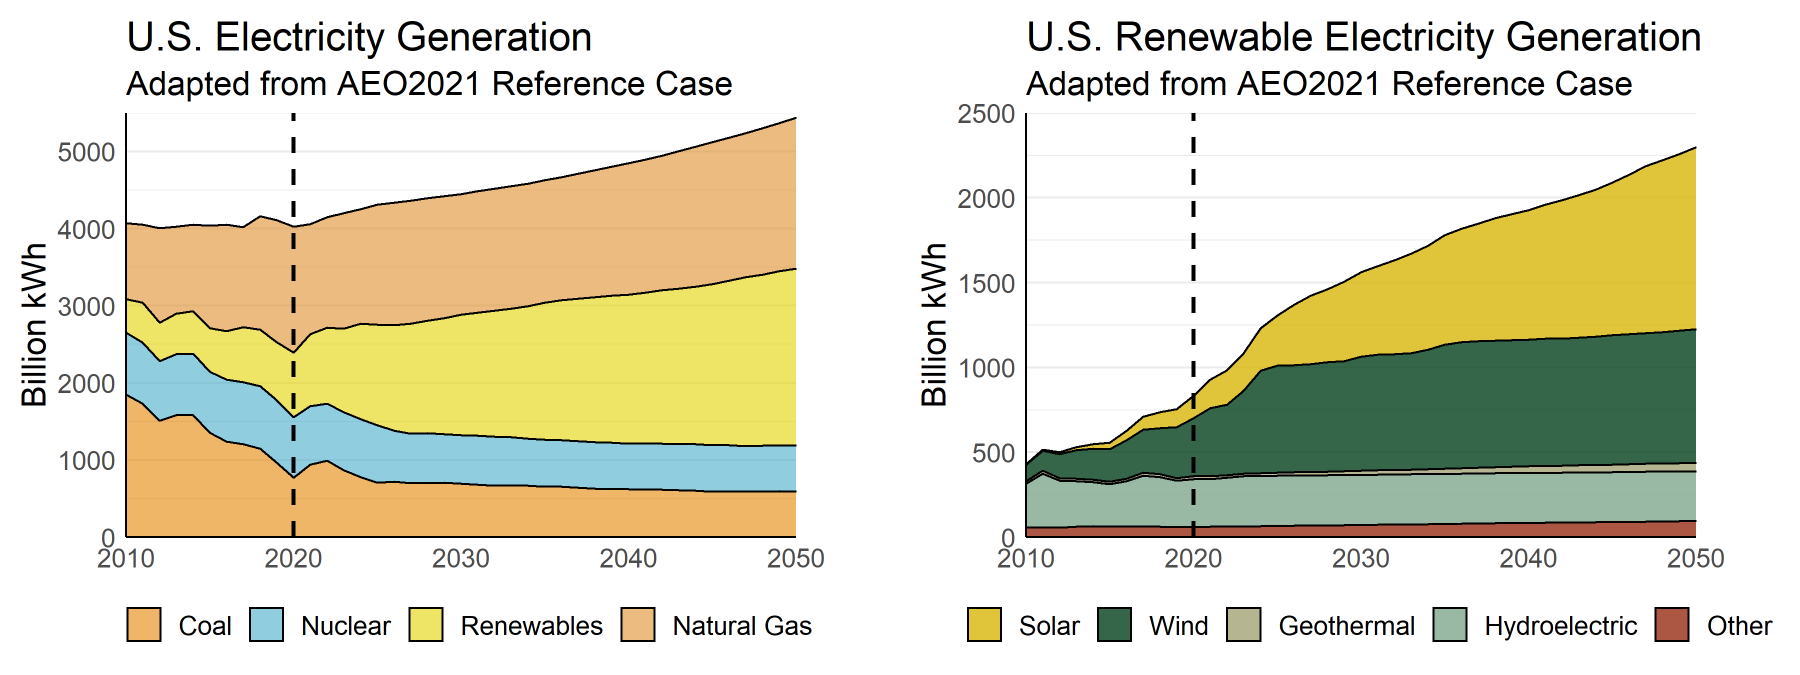
\includegraphics[width=\textwidth]{templates/images/Figure-EIA_projections.png}
\caption[U.S.\ EIA projections based on the AEO2021 reference case]{U.S.\ EIA projections of (Left) U.S.\ electricity generation by fuel source and (Right) individual contributions by renewables based on the AEO2021 reference case \protect\citep{eia_annual_2021}. Vertical dashed line marks where historical records end and projections begin.}
\label{fig:eia_2021_projections}
\end{figure}

Lazard Asset Management breaks renewables down by \acrlong{lcoe} (\acrshort{lcoe}) in U.S.\ dollars/MWh, where \acrshort{lcoe} is the estimated lifetime average net cost per unit energy of an electricity-generating plant. In their 2020 analysis, intermittent energy sources like wind and utility-scale solar are already cost-competitive with fossil fuel-derived sources (Figure \ref{fig:lazard_lcoe}) \citep{lazard_lazards_2020}. Geothermal, an “always on” source of power, ranges from \$59-\$101/MWh LCOE, making it second-tier in cost-competitiveness but comparable to community and rooftop solar installations \citep{lazard_lazards_2020}. Overall, the transition away from fossil fuel super-dominance is in progress, and the demand for energy in support of population growth and country development will remain an industry driver over the next 30 years.
 
\begin{figure}[htp]
\centering
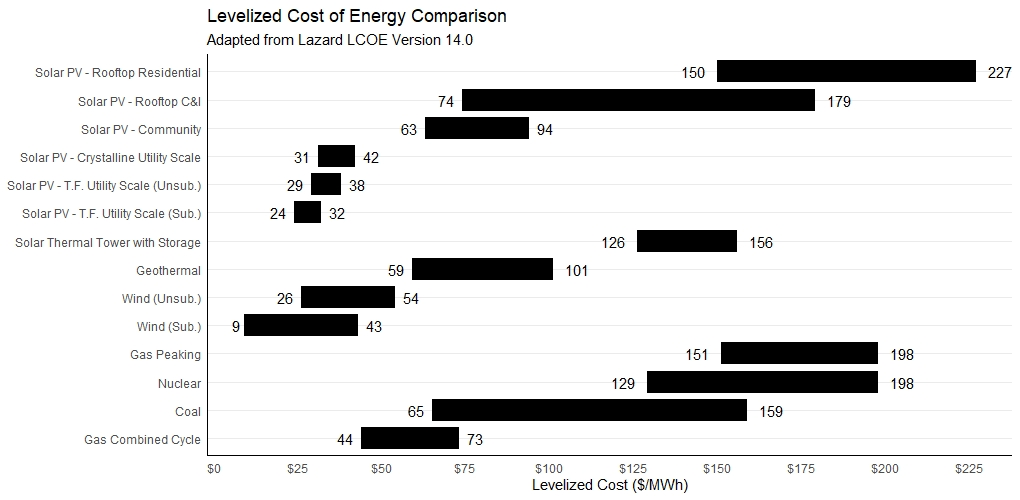
\includegraphics[width=\textwidth]{templates/images/Figure-Lazard_LCOE_recreated.jpeg}
\caption[Lazard Levelized Cost of Energy 2021 projections]{Cost comparison between different energy sources based on Lazard Asset Management LCOE analysis. C\&I: Commercial \& Industrial, T.F.: Thin Film, Unsub.: Unsubsidized, Sub.: Subsidized. For specific assumptions and caveats related to the analysis, see \protect\citep{lazard_lazards_2020}.}
\label{fig:lazard_lcoe}
\end{figure}

\section{Upstream Commercial Pressures}\label{ch1:upstream}
Businesses focused on exploration and production of oil \& gas face a growing list of pressures influencing future corporate strategy. On one hand, the increase in energy consumption predicted by the AEO and IEO supports a steady increase in production to meet global demand; however, geopolitical tensions, state-ownership of oil companies, and breakthrough technologies create a volatile landscape unforgiving of an unsophisticated production approach. In just the past 15 years, major downturns in oil prices were triggered by a mixture of factors: the financial crisis, tied to banking practices and housing market instability in 2008 \citep{singh_2007-2008_2021}; increased production from U.S.\ unconventional plays and supply decisions from the Organization of the Petroleum Exporting Countries (OPEC) in 2014 \citep{lioudis_what_2021}; and a price war between Russia and Saudi Arabia coinciding with a global pandemic in 2020 \citep{blessing_what_2021}. Additional uncertainty comes from National Oil Companies (NOCs) that control the majority of the world’s petroleum reserves, production, and rights for exploration and development. NOCs operate under different business drivers than International Oil Companies (IOCs), with ramifications on the stability of IOC investments and access to reserves as seen in Russia and Venezuela \citep{bremmer_long_2010,pirog_role_2007}. Meanwhile, disruptive technologies like precise directional drilling and efficient hydraulic fracturing have freed access to previously cost-prohibitive reserves, changing the balance of power as countries like the U.S.\ and China become less reliant on foreign hydrocarbon imports \citep{shuen_dynamic_2014}.

Layered on top of these macroeconomic influences are unexpected events that have enormous impact on energy production and distribution operations. The 2020 outbreak of COVID-19 acted as an accelerator on longer-term trends of digital transformation and decarbonization in the oil \& gas industry. In the wake of a 25\% decrease in global demand, companies responded with massive layoffs and restructuring, a heightened focus on digitalization, and portfolio rationalizations that include shale write-downs and asset divestments \citep{deloitte_2021_2020}. Also, extreme weather events consistent with global warming predictions are shining a critical spotlight on how energy is managed now and in the future. Blackouts, water outages, and surge pricing on electricity impacted millions of Texans in February 2021 when a winter storm brought record cold temperatures, exposing systematic weaknesses in energy infrastructure and generator preparedness for low-probability but feasible working conditions \citep{harc_winter_2021,lazard_lazards_2020}. And additional threats loom in the cyberworld as malicious hacking activities have rippling social and financial implications. One such attack on Colonial Pipeline, which handles almost 50\% of the liquid fuels supplied to the U.S.\ East Coast, led to gasoline shortages, price spikes, chemical factory shut-downs, and worldwide news coverage until the nearly \$5 million in ransom was paid in May 2021 \citep{sanger_pipeline_2021}.

\section{Net Zero Ambitions}\label{ch1:netzero}
The 2015 Paris climate agreement set a target of $<2^\circ$C on the rise in global temperatures above the pre-industrial average (i.e., the period from 1850-1900) to prevent the most extreme impacts of climate change \citep{unfccc_paris_2015}. The more commonly-ascribed $1.5^\circ$C target may be unachievable given current trajectories, and international calls to action are focusing on reducing anthropogenic carbon dioxide emissions to ``net zero'' as quickly as possible \citep{ipcc_global_2018}. Greater public awareness about the environmental impacts of global warming and alignment with these targets is putting pressure on the energy industry to revise their traditional business models. Beginning in 2020, top-tier oil and gas companies started issuing press releases outlining energy transition targets for 2025, 2030, 2050, and beyond \citep{bp_international_2020,chevron_chevron_2021,conocophillips_conocophillips_2020,equinor_equinor_2020,exxonmobil_exxonmobil_2021,shell_responsible_2020,shell_shell_2021,total_total_2020,total_2020_2021}. The proposed strategies vary but generally focus on (i) reducing company stake in fossil-fuel exploration and production activities, (ii) setting a net zero target applicable to emissions from operations, product carbon intensity, and carbon offsets, and (iii) dedicating investments in low- and no-carbon energy alternatives to replace hydrocarbons. Nevertheless, the pressure to do more, faster reached a new peak in May 2021 when a court decision in The Netherlands and approved shareholder proposals for two U.S.\ majors demanded an accelerated push toward emissions reductions and low-carbon energy options \citep{mcwilliams_investors_2021}.

\section{Geothermal Energy}\label{ch1:geothermal}
Several factors must be met for an energy source to be considered a viable and sustainable alternative to the carbon-based fuels (coal, natural gas, oil) that currently meet much of the world’s energy needs. \citeauthor{glassley_geothermal_2015} outlines a succinct set of criteria for such an energy resource: i) self-replenishment, ii) adequate abundance to meet energy demands, iii) low- to no-greenhouse gas emissions, and iv) cost competitiveness compared to accessible alternatives (\citeyear[p.\ 7]{glassley_geothermal_2015}). The first criterion precisely characterizes renewable sources of energy like solar, gravitational, and geothermal. Solar energy includes both direct (sunlight) and indirect (wind, waves, water cycle) resources \citep{hohmeyer_ipcc_2008}. Gravitational energy drives the tides and supports energy-storage solutions like pumped-storage hydropower \citep{eere_pumped-storage_2021,hohmeyer_ipcc_2008}. And geothermal energy is derived from accretionary heat and natural decay of radioactive isotopes within the Earth \citep{hohmeyer_ipcc_2008}. Table \ref{tab:renewableflux} specifically addresses criterion ii; the annual abundances of most renewable sources exceed energy demand, with geothermal scaling several orders of magnitude greater in annual flux/demand than other options \citep{hohmeyer_ipcc_2008}. Geothermal also meets the third criterion by providing a no-carbon source of energy that could support net zero aspirations when used in place of fossil fuels. The fourth criterion is less clear-cut. Geothermal costs depend strictly on use case, but as noted in Section \ref{ch1:trends}, LCOE analysis currently ranks geothermal below wind and solar in the list of renewable options \citep{lazard_lazards_2020}. Does this make geothermal non-viable as an alternative? Perhaps no, as geothermal comes with several unique opportunities and benefits.

\begin{table}[h!]
\centering
\begin{tabular}{|l|l|l|}
\hline
\textbf{Renewable Source} & \textbf{Annual flux (EJ/yr)} & \textbf{Annual Flux/Demand*} \\ \hline
Solar      & 3,900,000   & 8,700  \\ \hline
Wind       & 6,000       & 13     \\ \hline
Hydro      & 149         & 0.33   \\ \hline
Bioenergy  & 2,900       & 6.5    \\ \hline
Ocean      & 7,400       & 17     \\ \hline
Geothermal & 140,000,000 & 31,000 \\ \hline
\end{tabular}
\caption[Annual renewable energy fluxes]{Annual renewable energy fluxes, adapted from Table 1 of \protect\citep{hohmeyer_ipcc_2008}. The (*) indicates flux/demand ratio is derived from global demand estimates.}
\label{tab:renewableflux}
\end{table}

Most fundamentally, geothermal energy offers a reliable, nearly inexhaustible resource accessible anywhere around the world. Unlike wind and solar, which depend on favorable locations and vary with both season and time of day, geothermal is ubiquitous and continuous. Furthermore, it can provide baseload power for regional electrical grids without the additional need of assistive energy-storage technology \citep{tester_future_2006}. Based on history, one might assume geothermal only works under conventional hydrothermal conditions, e.g., near active volcanoes (e.g., Iceland, Indonesia) or within major rift zones (e.g., East African Rift). However, additional opportunities lie in low-temperature direct-use geothermal for heating and cooling of buildings, industrial processing, agricultural activities, and manufacturing \citep[p.\ 9]{glassley_geothermal_2015}. And technology supporting Enhanced Geothermal Systems (EGS) provides access to subsurface heat in areas without hydrothermal conditions \citep{tester_future_2006}. Natural radioactive decay takes place throughout the Earth’s crust, contributing to the global rise in temperature with depth known as the geothermal gradient \citep[p.\ 279]{fowler_solid_2005}. Where conditions permit access to suitable depths, there is the potential for geothermal energy capture.

For all its benefits, the use of geothermal energy comes with a set of challenges that are unique among renewable energy options. Many mirror issues faced by oil \& gas producers, like failures in drilling equipment or borehole integrity. Others include risk of low resource quality, poor reservoir productivity, unexpected structural and stratigraphic complexity, and undesirable fluid chemistry \citep{beckers_low-temperature_2016, hadi_resource_2010}. The similarities extend into unconventionals/EGS, where hydrofracturing risks comprise inadequate permeable rock volume within the stimulated fracture zone, short-circuiting of fluid flow between injection and productions wells, fluid losses within the subsurface, and induced seismic activity \citep{jelacic_evaluation_2008,pan_establishment_2019}. As in oil \& gas projects, some of these risks can be mitigated through appropriate subsurface characterization, others from high-resolution reservoir and fracture modeling. Collectively, the overlap in operational challenges and the skill sets required to tackle them defines a unique compatibility between oil \& gas and geothermal. Knowledge transfer between the two domains could directly benefit geothermal operations and risk-mitigation strategies \citep{petty_synergies_2009}. And investing in geothermal assets could take upstream companies a step closer to meeting net-zero commitments while retaining and utilizing existing talent.

One of the most significant uncertainties for geothermal is cost. The scope of an LCOE assessment considers all costs in a geothermal project, from early exploration, through development drilling and power plant construction, to operations and maintenance over a 25- to 30-year lifetime \citep{beckers_introducing_2013, entingh_volume_2006, tester_economic_1990}. Studies show drilling of exploration, appraisal, injection, and production wells can account for 60-75\% of the total EGS project expenses \citep{lukawski_uncertainty_2016, petty_synergies_2009}. New technologies being developed may help address future drilling costs \citep{lowry_geovision_2017,nrel_2020_2020}. However, substantial project savings could also be achieved through better characterization prior to drilling the first exploration well; increasing the probability of well success without multi-million dollar well failures would certainly reduce LCOE. In addition, choices in the design of the geothermal power plant may also have significant cost implications over the life of a geothermal field. Lessons can be learned from power plants built to design specifications incompatible with actual production conditions \citep[e.g.,][]{manente_hybrid_2011}. Improving the economics of geothermal start with recognizing uncertainties in the system and using those uncertainties to make better decisions on \textit{where to drill} and \textit{how to produce}. Providing the appropriate tools and methods to make these decisions could also help oil \& gas companies manage the risk of embracing lower-carbon energy production with geothermal as part of their energy mix.

\section{Research Questions}\label{ch1:researchqs}
Based on the above-mentioned opportunity to define methods that incorporate uncertainty characterization for risk management in geothermal exploration and production, this thesis will address the following research questions:

\begin{enumerate}
  \item Can geothermal exploration risk be mitigated by insights derived from readily-available data sources with little change in project cost? Can the data establish additional actions for further risk reduction before drilling a geothermal well? 
  \item How can characterization of present and future uncertainties influence the development and production strategy for geothermal facilities? In what ways will such an approach mitigate risk, if at all?
\end{enumerate}

\hfill\break
\section{Thesis Outline}\label{ch1:outline}
This thesis follows the flow shown in Figure \ref{fig:thesis_flow} and is structured as follows: 
\begin{figure}[!htp]
\onehalfspacing
\begin{minipage}[b]{0.5\textwidth}
\begin{itemize}
\item Chapter 2 provides relevant background material on geothermal systems, a literature review on geothermal exploration and cost modeling, and a primer on case study areas investigated in later chapters.
\item Chapters 3--4 describe the thesis data sources, data preparation strategies, and the chosen methods for favorability prediction with machine learning (Ch.\ 3) and cost modeling of geothermal project designs (Ch.\ 4).
\item Chapters 5--6 describe the machine learning model results (Ch.\ 5) and cost modeling results (Ch.\ 6).
\item Chapter 7 frames learnings from the previous chapters as risk mitigation actions in an overall risk management workflow.
\end{itemize}
\end{minipage} \hfill
\begin{minipage}[b]{0.47\textwidth}
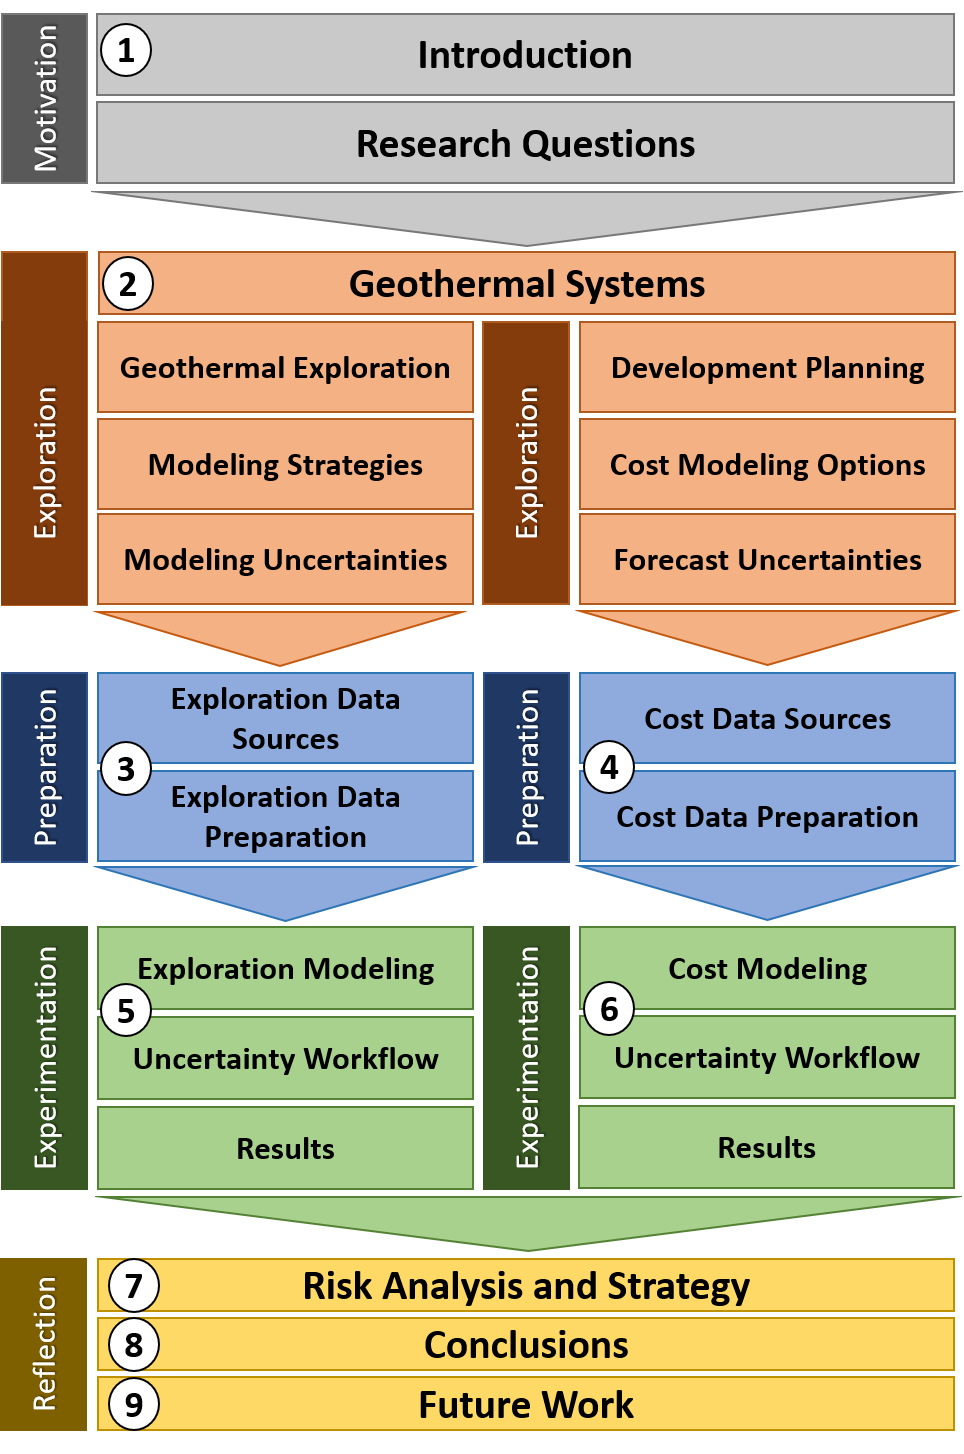
\includegraphics[scale=0.47]{Figure-ThesisWorkflow}
\caption[Thesis structure flow chart]{Flow chart of thesis structure. Chapter numbers are circled.}
\label{fig:thesis_flow}
\end{minipage}
\begin{itemize}
\item Chapters 8 and 9 conclude the thesis with a summary of thesis insights (Ch.\ 8) and a list of future work opportunities (Ch.\ 9).
\end{itemize}
\end{figure}
\chapter{Background}\label{ch2:background}

\section{Geothermal Systems}\label{ch2:geosys}
\subsection{Heat Origins}\label{ch2:heatorig}
\subsubsection{Accretion}\label{ch2:accrete}
The story of geothermal energy begins with the birth of planet Earth. Approximately 4.56 billion years ago \citep{allegre_age_1995, patterson_age_1956}, the Earth coalesced as a molten body heated by repeated impacts with objects in the early solar system like the planetesimal impact responsible for the formation of the Moon \citep{stevenson_origin_2014}. Over tens of millions of years, the Earth compacted, cooled, and differentiated, settling into the familiar layered structure of a solid inner core, liquid outer core, viscous mantle, and outermost brittle crust \citep[~p. 7]{press_understanding_2004}. The intense heat from that early accretionary history remains concentrated in the core, where temperatures - a matter of continued scientific inquiry - fall in the range of 6000±500 K \citep[~p. 372]{fowler_solid_2005}. Present day heat flux estimates for the whole Earth amount to 87 mW/m\textsuperscript{2}, \texttt{\char`\~}60\% of which flows through conductive and convective pathways from the deep interior to outermost crust \citep{stein_heat_1995}. Diffuse conductive heat transfer occurs everywhere across of the Earth’s surface, but heat flow concentrates along tectonic plate boundaries. In fact, the subduction-sourced volcanoes that ring the Pacific Ocean, divergent zones at the mid-ocean ridges and East African rift, and major strike-slip boundaries like the San Andreas fault zone all mark locations where focused heat anomalies are already being tapped by geothermal installations \citep[~p. 16]{dipippo_geothermal_2012}.
\subsubsection{Radioactive Decay}\label{ch2:radio}
The second major source of heat within the Earth is the decay of radioactive isotopes. Early radioactive heating included radioisotopes with short half-lives like Aluminum-26 and Hafnium-182, which are now no longer present \citep[~p. 16]{glassley_geothermal_2015}. Among the radioactive elements contributing the most to heating the crust today are uranium (U), thorium (Th), rubidium (Rb), and potassium (K) \citep[~p. 17]{glassley_geothermal_2015}. The decay of these and other elements accounts for 40\% of the crustal thermal budget \citep{stein_heat_1995}. But element abundances are not distributed uniformly throughout the crust. On average, continental crust, particularly the upper continental crust, has significantly higher concentrations of U, Th, and K radioactive elements compared to oceanic crust, and both types of crust are 1-2 orders of magnitude more enriched than the mantle \citep[~p. 276]{fowler_solid_2005}. This relationship holds for representative igneous rock types; granite generates more heat than basalt, and both out-produce ultramafic rocks like peridotites \citep[~p. 276]{fowler_solid_2005}.
\subsection{Heat Measurements}\label{ch2:heatmeas}
\subsubsection{Geothermal Gradient}\label{ch2:geotherm}
Average subsurface conditions show a steady increase in temperature with depth, commonly referred to as the geothermal gradient, sustained by the flow of original accretionary heat and generated radioactive heat. On average, the gradient for continental crust is \texttt{\char`\~}30\textdegree C/km \citep[~p. 209]{press_understanding_2004}. However, deviations from this value are common and reflect the complexity of the rock record in an area. The crust comprises a distinct set of layers, or strata, that vary in composition and rock type. Unlike the aforementioned igneous formations that can be relatively homogeneous, surface processes mix sediments from a variety of original source rocks, sometimes sorting them well and sometimes not, before they get deposited and indurated into sedimentary formations \citep[~p. 164-168]{press_understanding_2004}. Alteration from fluids, heat, and pressure can then modify the composition of these rocks, causing constituent minerals to change form and arrangement to create metamorphic rocks \citep[~p. 195-205]{press_understanding_2004}. The spatial and depth variations in these formations create subsurface compositional heterogeneity, directly reflected in rock properties. Thermal conductivity, specifically the ability to move deep-sourced heat to shallower depths, and radioactive element abundance, or the ability to generate additional heat in situ, can therefore vary in all directions in the subsurface. Thermal heterogeneity can be further compounded by anomalies created from salt movement \citep[~p. 164-168]{press_understanding_2004}, magmatic intrusions, or global tectonic processes. It therefore takes a good understanding of the geology and geologic history to determine the geothermal gradient of a region.
\subsubsection{Heat Flow}\label{ch2:heatflow}
Fundamentally, heat moves from hot to cold (Second Law of Thermodynamics) at a rate that linearly scales with the thermal gradient. Simple, one-dimensional thermal conduction can be characterized by the relationship \citep[~p. 270]{fowler_solid_2005}:
\begin{equation}\label{eq:conduction}
q = -k \frac{\nabla T}{x}
\end{equation}
where q is heat flux, or heat flow per unit time per unit area, with S.I. units of \(Wm^{-2}\). Heat flux depends on the gradient of temperature (T), the distance over which conduction takes place (x), and the thermal conductivity (k), that is, the ability of material to conduct heat. Different rock types have different values of k, e.g., sandstone varies from 1.60-2.10 \(W/m^\circ C\) while granite tends to be higher with values ranging from 1.73-3.98 \(W/m^\circ C\) \citep[~p. 30]{dipippo_geothermal_2012}. Feldspars and quartz exhibit significant (up to 3x) differences in k values. As the most abundant minerals in crustal rocks, their relative fractions will strongly influence the thermal conductivity of a formation \citep[~p. 22]{glassley_geothermal_2015}. Regardless, minerals tend to be relatively poor thermal conductors compared to other materials like aluminum (210 \(W/m^\circ C\)) and iron (73 \(W/m^\circ C\)), making conduction a slow method of crustal heat transmission \citep[~p. 23]{dipippo_geothermal_2012}.

Conduction dominates on local scales in the crust, while convection is the primary means of heat transfer on global, tectonic scales. Even in its two-dimensional form with no internal heat generation, the equation governing convection is much more complex than for conduction \citep[~p. 355]{lowrie_fundamentals_2007}:
\begin{equation}\label{eq:convection}
\frac{\partial T}{\partial t} = \left (\frac{k}{\rho * c_P}\right)\left (\frac{\partial ^2T}{\partial x^2}+\frac{\partial ^2T}{\partial z^2}\right)-u_x\frac{\partial T}{\partial x}-u_z\frac{\partial T}{\partial z}
\end{equation}
where \textbf{u} = \(( u_x, u_z)\) is the velocity of the fluid, \(\rho\) is the material density, and \(c_P\) is the specific heat, which defines the amount of heat necessary to raise 1 kg of that material by 1\(^\circ C\) Convention combines heat transfer from conduction with mass movement. Since the minerals are relatively poor conductors of heat, the combined effects of lower viscosity and thermal expansion – as seen near the core-mantle boundary – and gravitational forces that create buoyancy effects, all create the right conditions for convective flow, e.g. within the mantle \citep[~p. 25]{glassley_geothermal_2015}. Mantle convection is responsible for the high heat flow values observed at crustal plate boundaries like mid-ocean ridges, as well as intraplate diapiric hot spots underlying Hawaii, Yellowstone, and a number of other locations around the world.  Smaller-scale convection also takes place at subduction zones where the material from the down-diving plate melts at lower temperatures with the presence of water, migrates upwards, and forms volcanic arcs on the surface as observed in Japan, Indonesia, and the Pacific Northwest of the U.S. \citep[~p. 31-33]{press_understanding_2004} – all locations with geothermal potential.

Heat flow measurements capture the flux of heat through the Earth’s surface as a result of these and other complex processes taking place in the subsurface. In this respect, it serves as a simpler and more accessible metric for local or regional heat potential than the more sparsely-measured and less well-constrained geothermal gradient. Today, high-quality heat flow measurements can be obtained in marine conditions, on continental margins, on mid-ocean ridges, and from the multitude wells drilled by the oil \& gas industry, supporting the creation of large heat flow data sets like the New Global Heat Flow database \citep{lucazeau_analysis_2019}. As Figure \ref{fig:heatflow} shows, data from these collections can be gridded to create spectacular maps of heat flow variations around the world. These maps offer a good starting point for quickly targeting where the greatest geothermal potential exists at the regional or “play” scale, which can then be further refined through additional methods (see Section \ref{ch2:geoexp}).
\begin{figure}[h!]
\centering
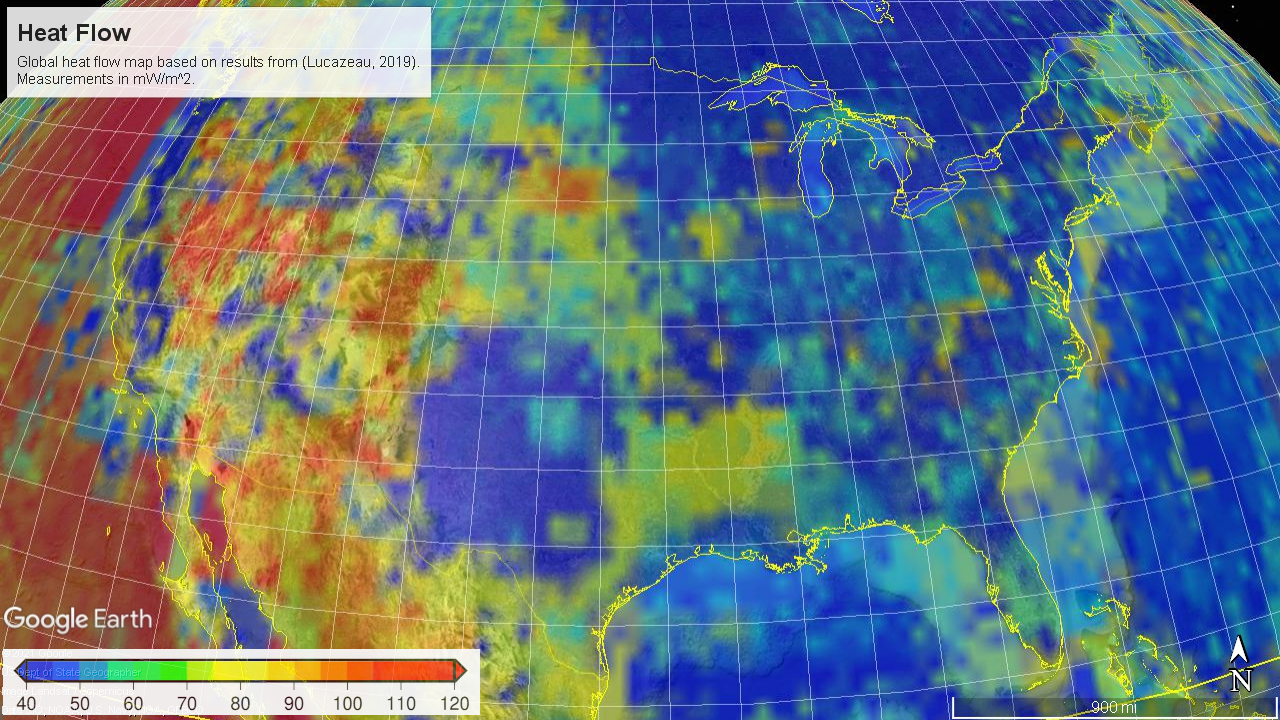
\includegraphics[scale=0.45]{Figure-HeatFlowMap}
\caption[Heat flow across the continental U.S.]{Heat flow estimates for the continental United States, plotted in Google Earth with data layer from \protect\citep{lucazeau_analysis_2019}}
\label{fig:heatflow}
\end{figure}
\subsection{System Fundamentals}\label{ch2:sysfund}
The conventional concept of a geothermal system consists of five key entities \citep[~p. 9]{dipippo_geothermal_2012}:
\renewcommand{\labelenumi}{\roman{enumi}}
\begin{enumerate}\label{list:sysreq}
   \item Heat source of significant size and temperature
   \item Permeability, typically in the form of a fracture network within crystalline rock
   \item Ample volume of working fluids, e.g. water from precipitation and drainage
   \item Impermeable sealing layer
   \item Consistent, reliable fluid recharge
\end{enumerate}

\subsubsection{Hydrothermal Systems}\label{ch2:hydro}
If naturally present, the combination of these five elements defines a hydrothermal system. As water percolates down, captures heat from the permeable thermal reservoir, and gets trapped beneath the sealing caprock, a small fraction of the resource can escape to the surface to produce distinctive geothermal manifestations like fumaroles, hot pools, geysers, mud pots, and discolored or altered rocks (Figures \ref{fig:lassen-geysers} and \ref{fig:lassen-mudpot}). These features are strong indicators of hydrothermal resources at depth.
\begin{figure}[h!]
\centering
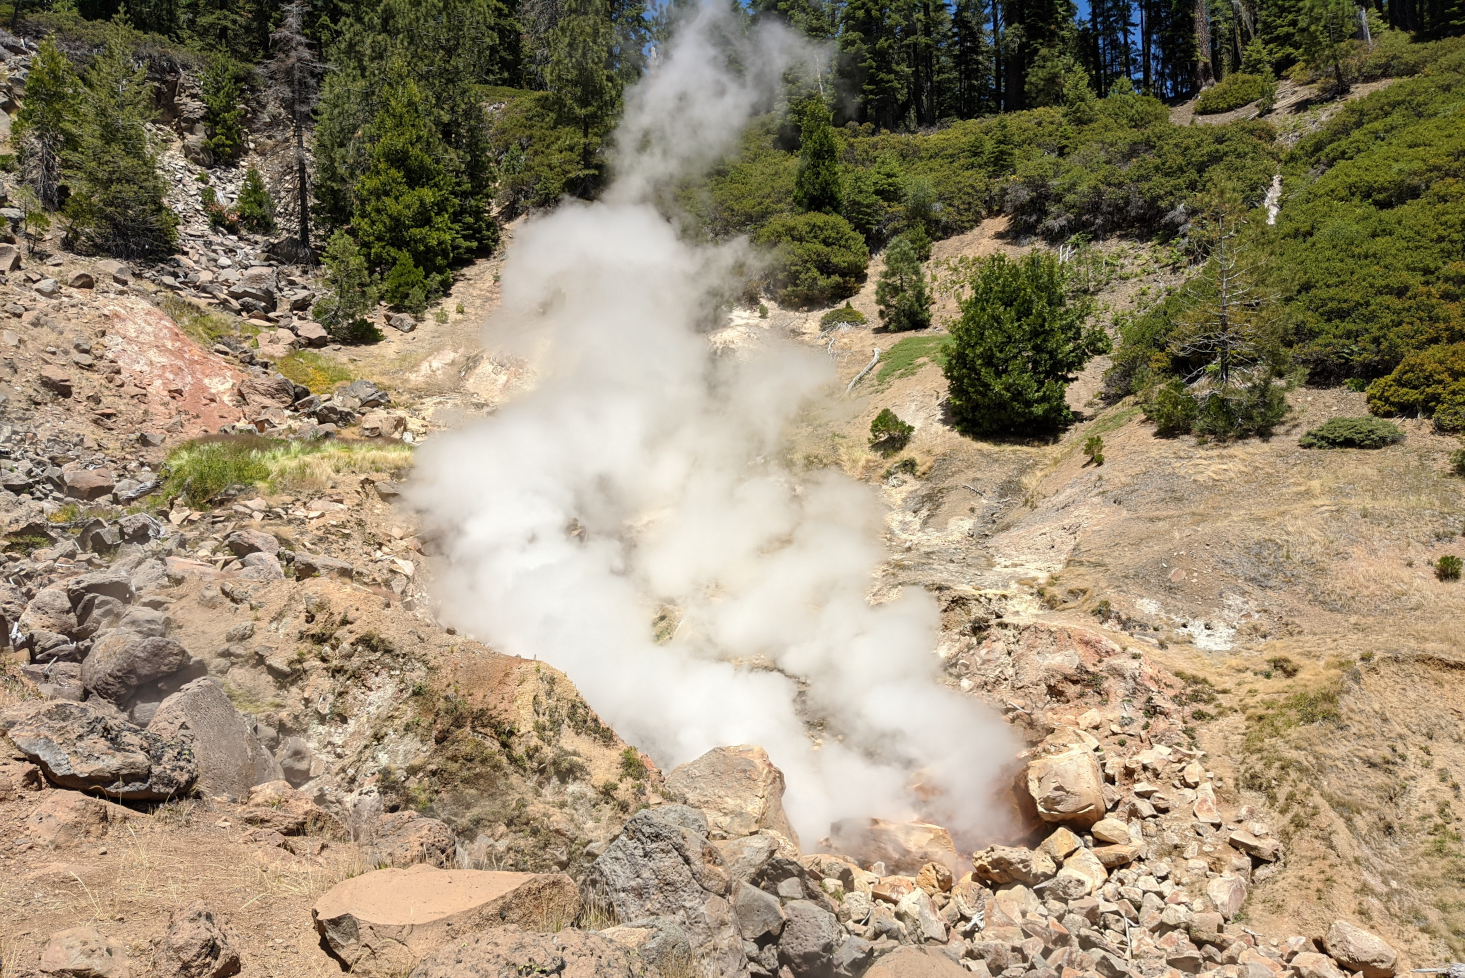
\includegraphics[scale=.84]{Figure-Lassen-geysers3}
\caption[Terminal Geyser, Lassen National Park]{Terminal Geyser, Lassen National Park, California. Photo credit: Author}
\label{fig:lassen-geysers}
\end{figure}
\begin{figure}[htbp]
\centering
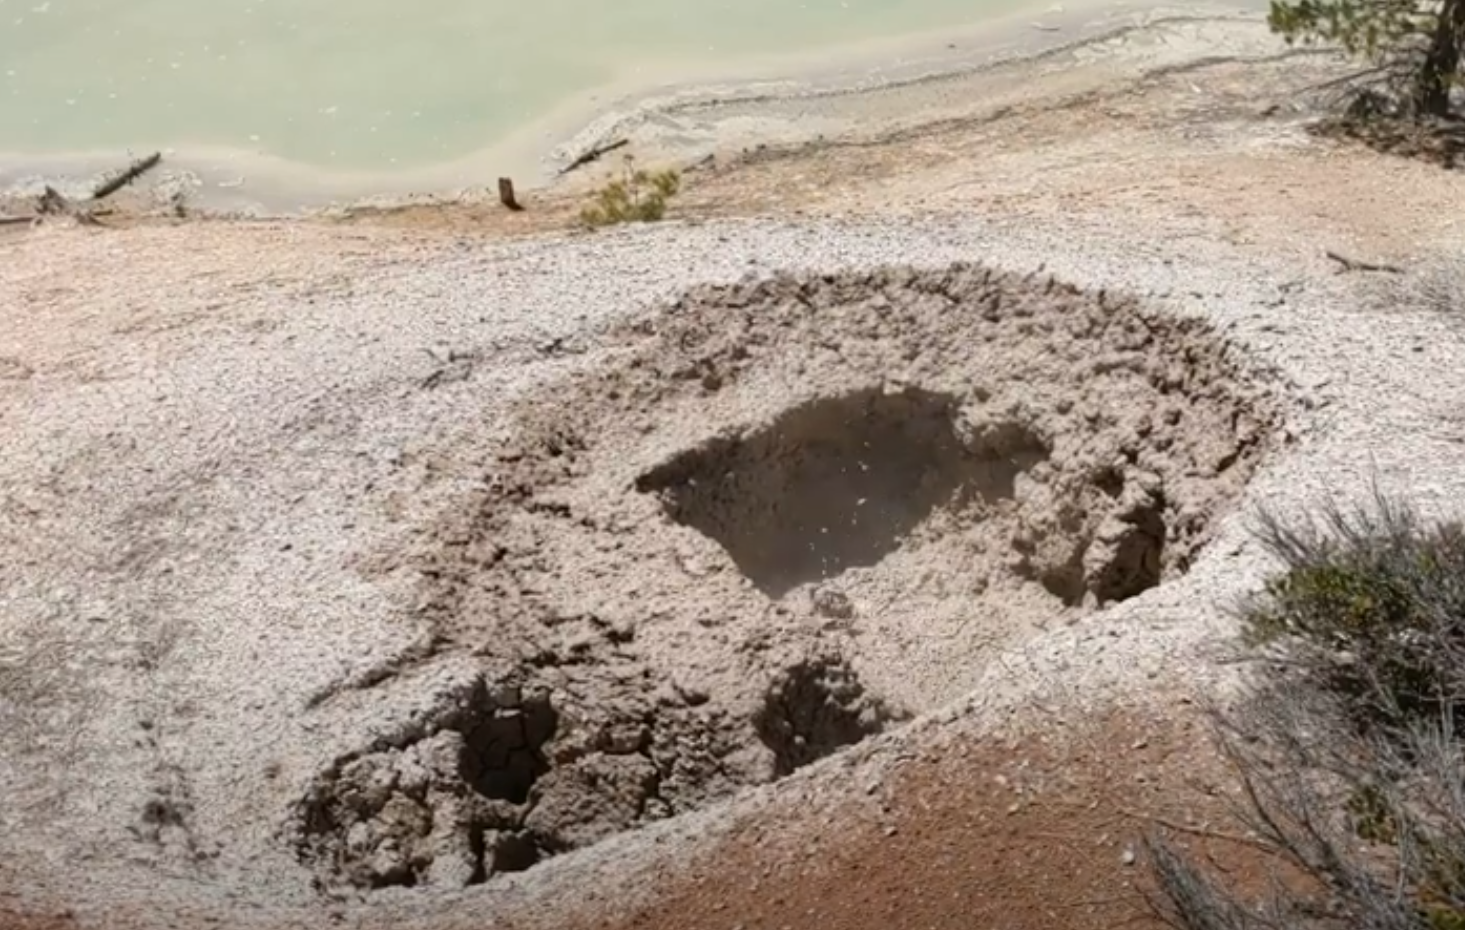
\includegraphics[scale=0.27]{Figure-Lassen-mudpot}
\caption[Mud pot, Lassen National Park]{Active mud pot and ground staining on the bank of Boiling Springs Lake, Lassen National Park, California. Photo credit: Author}
\label{fig:lassen-mudpot}
\end{figure}
The original geothermal systems exploited by mankind for millennia are hydrothermal systems. Artifacts show proto-Native American use of hydrothermal waters for cleaning and health restoration over 10,000 years ago \citep{doe_history_2021}. The importance of geothermal hot springs for Roman, Japanese, Chinese, and Ottoman baths is also well-established in the historical record \citep{lund_characteristics_2007}. Industrial use began in the 1800s with chemical extraction from geothermal steam, pools, and deposits in Larderello, Italy \citep[~p. 251]{dipippo_geothermal_2012}. \acrlong{gdh} (\acrshort{gdh}), or large-scale heating of residences and businesses using geothermal-produced fluids, was pioneered in Chaudes-Aigues, France in the 1300s and first introduced to the United States in 1892 with an installation in Boise, Idaho \citep{lund_characteristics_2007}.

These few examples capture some of the many potential opportunities for low-temperature (<90\(^\circ C\)) and medium-temperature (<150\(^\circ C\)) geothermal resource use, even beyond hydrothermal systems. GDH can help meet building and water temperature needs, and agriculture, textiles, paper, chemicals, and even the food industry can also benefit from access to low-temperature geothermal fluids \citep{doe_low_2021,liu_overview_2015}. Interest has led to funding from agencies like the \acrlong{gto} (\acrshort{gto}) within the \acrlong{doe} (\acrshort{doe}); a grant was recently awarded to Cornell University in support of piloting a deep direct-use project to provide baseload heating for the university campus supporting peak demand during cold upstate New York winter months  \citep{hamm_geothermal_2021,tester_integrating_2015}.

The topic of this thesis instead concerns the use of moderate- to high-temperature geothermal for power generation. The first example of geothermal power production came from Italian experiments in 1904, and the first commercial plant went online in Larderello, Italy in 1914 \citep[~p. 251]{dipippo_geothermal_2012}. Geothermal-generated electricity made its debut in the United States with the development of The Geysers field beginning in 1960 \citep{tester_future_2006}. Hydrothermal plants quickly appeared in New Zealand, Japan, Iceland, Indonesia, Kenya, Philippines and elsewhere throughout the 1970s-1980s, with continued growth through to present-day \citep{lund_characteristics_2007}. 2020 statistics from the \acrlong{irena} (\acrshort{irena}) place the United States as world leader in geothermal installed capacity (2587 MWe), followed by Indonesia (2131 MWe) and Philippines (1928 MWe) \citep{irena_country_2021} (Figure \ref{fig:irena-rank}). 

\begin{figure}[htbp]
\centering
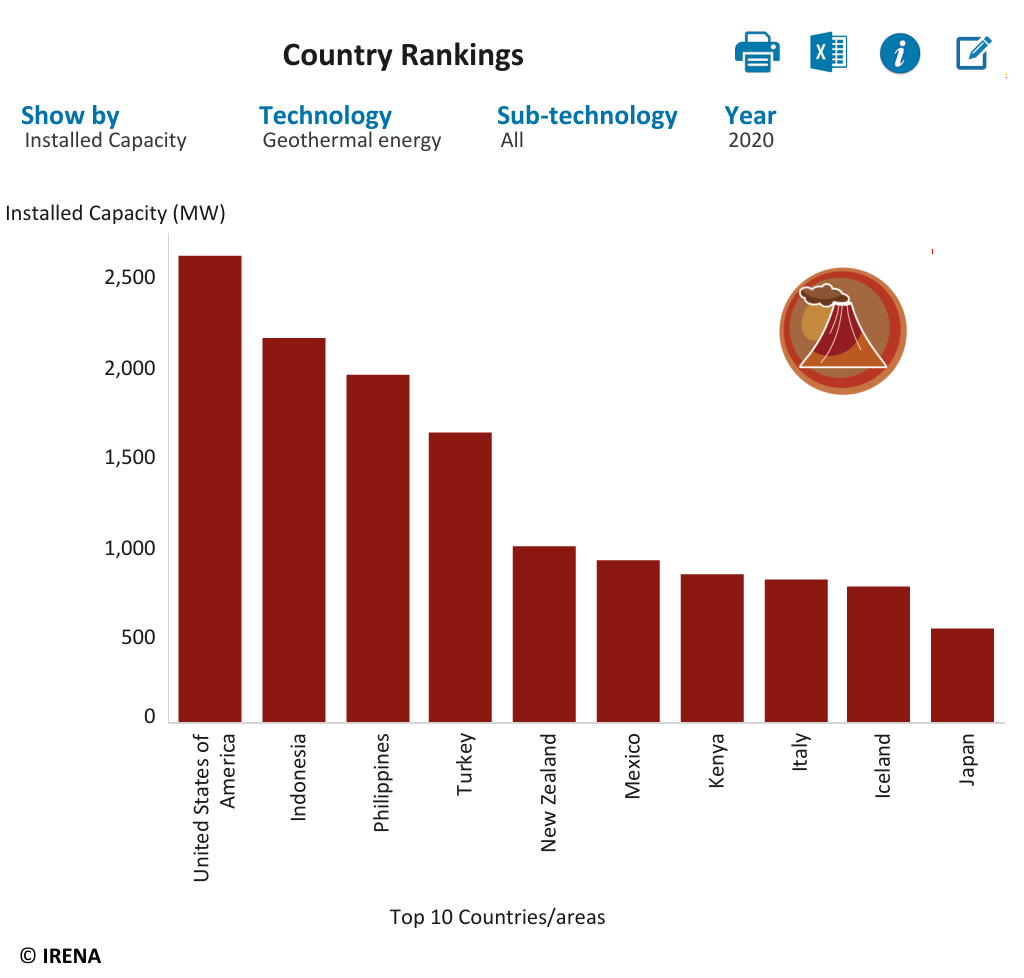
\includegraphics[scale=.45]{Figure-IRENA_Rankings}
\caption[Country rankings, installed geothermal capacity ]{Countries ranked by installed geothermal capacity, from \protect\citep{irena_country_2021}}
\label{fig:irena-rank}
\end{figure}

A comprehensive assessment of moderate and high-temperature \acrlong{kgra}s (\acrshort{kgra}s) by the \acrlong{usgs} (\acrshort{usgs}) determined the U.S. has conventional geothermal (hydrothermal) power generation potential of \texttt{\char`\~}9,000 MWe, and an additional \texttt{\char`\~}30,000 MWe potential exists in undiscovered resources \citep{williams_assessment_2008}. The recent DOE GeoVision study notes hydrothermal potential in Alaska and Hawaii alone are \texttt{\char`\~}8000 MWe due to their unique tectonic environments (Aleutian subduction zone and Hawaiian hot spot, respectively), and high-case model estimates for the continental U.S. forecast an installed capacity of \texttt{\char`\~}16.5 GW by 2050 for known and unknown hydrothermal resources \citep{augustine_geovision_2019,hamm_overview_2019}.

\subsubsection{Enhanced Geothermal Systems}\label{ch2:egs}
In some cases, the potential for a geothermal system exists even when one or more of the fundamental elements listed in Section \ref{ch2:sysfund} are missing. These unconventional geothermal systems, often referred to as \acrlong{egs} (\acrshort{egs}), contain a significant heat source but lack either the adequate permeability or sufficient rechargeable working fluids to meet the requirements of a hydrothermal system. A broader definition for EGS includes thermal production from sedimentary and crystalline tight rock, poorly-performing hydrothermal systems, co-production from oil \& gas operations, and even thermal recovery directly from magma \citep{tester_future_2006}. Focusing on the more common tight rock scenario, EGS systems work by artificially creating or improving reservoir permeability and ensuring sustained flow rates of fluids through the reservoir \citep[~p. 281]{glassley_geothermal_2015}. Fluids pumped down an injection well pass through a stimulated fracture network, heat up through direct contact with the thermal reservoir, and return to the surface via one or more producing wells to serve as inlet fluids for a power plant \textbf{MISSING FIGURE}. Reservoir stimulation generally involves hydraulic fracturing (hydro-fracking or just “fracking”) techniques to create pathways connecting injector-producer pairs. The associated technology and capabilities are thus well-aligned with unconventional oil \& gas operations \citep{petty_synergies_2009}. 

EGS can provide the bridge between geothermal use in niche hydrothermal environments and a more comprehensive adoption of geothermal energy for electricity generation across the United States. The sources of subsurface heat (see Section \ref{ch2:heatorig}) exist everywhere, so accessing a range of temperatures that could support power production relies on drilling deep enough and creating the artificial conditions necessary for heat capture. \acrlong{lanl} (\acrshort{lanl}) validated the EGS approach in crystalline rock at Fenton Hill beginning in 1974, soon after which feasibility studies were conducted in Japan, Germany, the U.K., and France \citep{breede_systematic_2013}. Among the most notable EGS projects that provided key lessons learned are The Geysers (U.S), Soultz-sous-Forêts (France), and Cooper Basin (Australia). The Geysers stands out as the largest geothermal power-generating complex in the world, providing \texttt{\char`\~}1,000 MWe for California even after 60 years of steam production \citep{jelacic_evaluation_2008,williams_assessment_2008}. Although drilling issues and public concern over induced seismicity halted efforts \citep{manish03_united_2009}, rock stimulation experiments in the Northwest Geysers proved distinct reservoirs can be developed adjacent to active hydrothermal operations \citep{pan_establishment_2019}. The Soultz project commenced in 1987 with one injector and two producers drilled to 5 km depth to support a 1.5 MW power plant built in 2007-2008 \citep[~p. 463]{dipippo_geothermal_2012}. In addition to many experimental lessons learned around drilling, hydrofracturing, chemical stimulation, scaling and corrosion, Soultz today supports both electricity production and direct-use district heating \citep{durst_overview_2013}. Cooper Basin, the largest EGS demonstration project in the world, showed great promise after a 6-year proof of concept phase \citep{stephens_assessing_2010}. However, the project halted in 2015 due poor stimulation results tied to an unrecognized fault, highlighting the importance of robust structural appraisal in assessing geothermal prospects \citep{holl_what_2015}. 

As the fate of these projects might suggest, the long-standing promise of EGS has not yet been fully realized. However, several active projects supported by the DOE and NREL (e.g. EDGE, FORGE, EGS Collab) are providing the insights necessary to mature subsurface models, drilling technologies, and stimulation methods for more widespread EGS adoption \citep{hamm_geothermal_2021}. And recent technology advances and partnerships involving start-ups Fervo Energy \citep{moss_google_2021,shieber_geothermal_2021}, Deep Earth Energy \citep{geoenergy_saskatchewan_2021}, Eavor Technologies \citep{ross_energy_2020}, and Climeon \citep{climeon_climeon_2021,geoenergy_baseload_2020} show there is a growing fervor to overcome the technology roadblocks currently holding EGS back. Projections show the size of the prize with success in EGS. Assuming a maximum cut-off depth of 7 km and a minimum reservoir temperature of 150\(^\circ C\), the EGS resource potential for electricity production in the continental United States might be at least \texttt{\char`\~}5,150 GWe, with an additional \texttt{\char`\~}1,500 MWe from NF-EGS \citep{augustine_geovision_2019}. To put this opportunity into context: the total utility-scale electricity generation capacity from \underline{all} sources in the United States was \texttt{\char`\~}1,200 GWe in 2019, over 4x less in magnitude \citep{eia_electric_2020}.

\section{Geothermal Exploration}\label{ch2:geoexp}
\subsection{Background}
Historically, the identification of geothermal resources primarily relied on surface expressions of hot fluids circulating at depth. Quite simply, if a bubbling hot spring or a geyser was present, you had a working hydrothermal system. Some of the first sites for geothermal power production, like Larderello and The Geysers, were unsurprisingly targeted because of their tell-tale surface characteristics \citep[~p. 111]{glassley_geothermal_2015}. However, this prospecting method only applies to fully-functioning hydrothermal systems, and not all such systems have surface manifestations if fluids remain trapped beneath a subsurface impermeable seal. These hidden or “blind” geothermal resources require more sophisticated exploration methods to identify and assess accurately.

\subsection{Regional Exploration}
Regional evaluation techniques classically relied on sparse borehole data, including water wells and oil \& gas wells, to map out the geothermal potential of the U.S. \citep{kehle_aapg_1970}. Successive efforts led to progressively more comprehensive collections of surface heat flow and borehole temperature measurements \citep{blackwell_temperature-at-depth_2011, blackwell_heat_1990, muffler_assessment_1979, sorey_low-temperature_1983, wisian_heat_1999}, now widely-available with other geothermal data through the DOE-funded National Geothermal Data System platform \citep{anderson_national_2013}. These efforts supported a better understanding of broad trends directly tied to tectonic provinces in the United States. Subduction and transform plate boundaries in the West, combined with extension in the Basin and Range, make this area of the U.S. more susceptible to high heat flow, high geothermal gradient, and greater potential for hydrothermal system activity \citep{mariner_low-temperature_1983}. Passive margins on the Atlantic and Gulf of Mexico sides make those regions less likely to host significant hydrothermal systems, although surveys have identified sedimentary basins with elevated heat flow in the south (Louisiana-Arkansas), central (Iowa-Illinois, Nebraska-South Dakota), and eastern (Appalachians) parts of the country \citep{blackwell_geothermal_1995, sorey_low-temperature_1983}.

\subsection{Sub-regional Exploration}
Continental maps provide a super-regional view of geothermal prospectivity, but further refinement is required to progress an exploration program. Specifically, the determination of regional plays and local prospects must come before deciding where and how to develop a geothermal field, e.g., for electricity generation. Characterization activities can be decomposed into defining the magnitude and extent of four earth subsystems: structural, stratigraphic, hydrologic, and thermal. The main types of surveys associated with each subsystem are listed in Table \ref{tab:surveytypes} and discussed briefly in the following section. Note that the various survey methods typically provide information on multiple subsystems. The associated non-uniqueness of subsurface interpretations based on these survey results highlights the need to integrate multiple lines of evidence for exploration activities. 

\begin{table}[!htp]
\begin{tabular}{ll}
\textbf{Structural}     & \textbf{}                                                \\ \hline
Aerial survey           & surface fault traces                                     \\
Earthquake records      & fault location, recency                                  \\
Geodetic survey         & active deformation or faulting                           \\
Geologic survey         & surface fault traces, fault recency                      \\
Gravity survey          & subsurface faults, plutons, salt                         \\
Resistivity survey      & fractured zones                                          \\
Satellite survey        & topography, structural patterns                          \\
Seismic surveys         & subsurface faults, folds, other structural features      \\
                        &                                                          \\
\textbf{Stratigraphic}  &                                                          \\ \hline
Geologic survey         & stratigraphic chart, seal and reservoir                  \\
Gravity survey          & density anomalies, stratigraphic variations              \\
Magnetic survey         & igneous formations, stratigraphy and reservoir           \\
Radiometric survey      & mineral abundances, source and reservoir                 \\
Resistivity survey      & thermal conductivity, lithology                          \\
Satellite survey        & distribution of outcrops and formations                  \\
Seismic survey          & stratigraphy and rock properties                         \\
                        &                                                          \\
\textbf{Hydrologic}     &                                                          \\ \hline
Earthquake records      & movement of magma or fluids                              \\
Geologic survey         & surface expressions (vents, geysers, deposits), drainage \\
Hydrologic survey       & fluid geochemistry, recharge and rate, water table       \\
Magnetic survey         & hydrothermal alteration                                  \\
Precipitation records   & water cycle inputs, recharge rate                        \\
Resistivity survey      & subsurface fluids or hydrothermal alteration             \\
Satellite survey        & surface drainage patterns, distribution of deposits      \\
Seismic survey          & presence and location of subsurface fluids               \\
                        &                                                          \\
\textbf{Thermal}        &                                                          \\ \hline
Aerial survey           & thermal anomalies in shallow subsurface (IR)             \\
Air Temperature records & near-surface thermal conditions                          \\
Geologic survey         & surface manifestations (dikes, vents, deposits)          \\
Gravity survey          & presence of high-T anomalies (e.g. magma)                \\
Hydrologic survey       & geothermometry, dominant geofluid liquid phase           \\
Radiometric survey      & radioactive heat generation                              \\
Resistivity survey      & thermal conductivity, temperature gradient               \\
Temperature survey      & heat flow, geothermal gradient                          
\end{tabular}
\caption{Data collection methods useful for characterizing and derisking Earth subsystems that influence geothermal favorability}
\label{tab:surveytypes}
\end{table}

\subsubsection{Geologic Data Collection}
Geologic field mapping in an area can provide crucial direct evidence supporting the presence of geothermal systems. Surface manifestations like geysers, vents, and mud pots may also be coincident with mappable mineralogic indicators of the subsurface chemistry and style of geothermal activity.  Volcanic-based geothermal systems tend to have acid-sulfate waters with hydrogen sulfide-rich brines that leave behind sulfur deposits \citep[~p. 123]{glassley_geothermal_2015}. Bicarbonate geothermal waters can produce distinctive travertine terraces or subaqueous tufa deposits, as well as a unique variety of K-spar called adularia \citep[~p. 125]{glassley_geothermal_2015}. And chloride geothermal fluids are known to precipitate sinter or geyserite deposits composed of opal or amorphous silica \citep[~p. 125]{glassley_geothermal_2015}. Elevated abundances of trace elements like boron and lithium typically occur in chloride brines compared to meteoric (derived from precipitation) waters, so their presence in mineral assemblages is also diagnostic \citep{bielicki_hydrogeolgic_2015, millot_multi-isotopic_2007}. Other valuable products of a geologic survey include maps of surface fault patterns to better constrain the structural history, as well as volcanic intrusive (dikes) and extrusive (flows) features for understanding the thermal history and potential deeper reservoir potential.

Direct geochemical analysis of springs, pools, and samples collected from wells provides additional insights into the hydrologic characteristics of an area. Water chemistry offers information on the dominant resource fluid phase (vapor vs. liquid), the temperature of the subsurface formations encountered by the fluids, and the nature of the original water source \citep[~p. 25]{dipippo_geothermal_2012}. The concentration or equilibria of different elements, e.g., quartz, chalcedony, sodium, potassium, and calcium, can be compared to empirically-derived trends for reservoir temperature estimates \citep[~p. 157]{glassley_geothermal_2015}. These geothermometry methods offer insights into the deep thermal regime, although uncertainty around fluid migration pathways disallows any clear designation of the exact location and depth of a thermal reservoir.

Field methods like water sampling and geologic mapping offer local insights that can be interpolated for a bigger picture understanding of an area, with the caveat that field data tend to be limited in both number and spatial distribution. Aerial and satellite surveys provide regionally extensive measurements without the spatial sampling bias implicit in field activities. High-resolution topography captured in \acrlong{dem} (\acrshort{dem}) and their gradient (slope) can reveal morphology patterns tied to surface water drainage and recharge potential for deeper geothermal systems. Other optical products provide additional information of value; infrared imagery captures thermal anomalies in the shallow subsurface, stereographic images emphasize fault offsets missed in the field, and hyperspectral imaging can discriminate between different mineral assemblages, including geothermally-sourced boron-rich accumulations \multicitep{dipippo_geothermal_2012, ~p. 22;glassley_geothermal_2015, ~p. 154-155}.

\subsubsection{Geophysical Data Collection}
Geophysical methods also offer regional data coverage while also providing insights into how subsurface characteristics vary with depth. Magnetic surveys detect the magnetic fields imprinted on rocks that contain susceptible minerals and have experienced appropriate thermal conditions \citep[~p. 248-249]{lowrie_fundamentals_2007}. Magnetic anomalies, calculated by removing the regional magnetic field and non-geologic signals, can indicate the presence of intrusive volcanic bodies or hydrothermally-altered formations \citep[~p. 146]{glassley_geothermal_2015}. Gravity surveys similarly consider variations in local values after applying a regional gravity removal and other corrections \citep[~p. 59-62]{lowrie_fundamentals_2007}. Gravity anomalies highlight differences in subsurface density, which may be diagnostic of mineral alteration from hydrothermal processes, the presence of fractures, or pore fluid changes (e.g., replacement of meteoric water with hydrocarbons, hydrothermal fluids, or steam) \citep[~p. 150]{glassley_geothermal_2015}. Resistivity surveys measure electrical resistivity (or its inverse, conductivity) within an instrumented area – a property sensitive to fluids in rock pores or fractures and some variations in mineralogy, i.e., within alteration zones \citep[~p. 147]{glassley_geothermal_2015}. However, poor resolution beyond shallow (~1 km) depths strongly limits the reach of classic resistivity studies. Magnetotellurics (MT), measurements of currents induced by natural electromagnetic waves originating in the ionosphere, can extend conductivity insights much deeper, even into the upper mantle \citep[~p. 225]{lowrie_fundamentals_2007}. And seismic surveys, which measure acoustic wave propagation in the subsurface, can be processed and modeled to image stratigraphy, faults, fluids, and rock properties to a range of depths. Seismic refraction data can constrain whole crustal thickness \citep[e.g.][]{holmes_oceanic_2009}, with implications on heat flow, while seismic reflection data could define the thickness and extent of a geothermal reservoir and trapping geometry \citep[e.g.][]{cappetti_new_2005}.

\subsection{Strategies}
\subsubsection{Joint Inversion}

As powerful as geophysical methods are at remotely detecting earth properties, each method represents an inherently underconstrained problem. Complex mathematical routines can invert data collected by aerial survey (e.g., gravity, magnetics) or through surface acquisition techniques (resistivity, MT, seismic) to create 2D or 3D subsurface models. Still, unlike highly precise medical imaging technologies like Magnetic Resonance Imaging (MRI) that completely surround the target, geophysical techniques have a limited top-down view of the earth and must contend with noisy environments. Solutions to geophysical problems thus tend to be non-unique, and uncertainty increases with depth. Joint approaches to mathematical inversion for subsurface models address this ambiguity by constraining solutions to match the observations from multiple geophysical methods at once \citep{vozoff_joint_1975}. The complexity of a joint inverse problem applied to geothermal rapidly grows as more data sets are incorporated, particularly when the different data are sensitive to different earth properties \citep{moorkamp_framework_2011}. In addition, geothermal model results can meaningfully differ depending on the selected mathematical treatment used to generate solutions \citep{rosenkjaer_comparison_2015}. One alternative approach avoids the mathematical and computational demands by combining data semi-quantitatively, either by visually correlating individual model results or by cascading constraints from one geophysical model to the next to generate an integrated solution \citep{jousset_hengill_2011, lichoro_joint_2019}. Absent a tightly-coupled formulation of the relationship between all data inputs, the weighted influence of each data source must be chosen by the analyst, which can be a significant source of uncertainty.

\subsubsection{Play Fairway Analysis}

Regional or play scale exploration methods adapted from oil \& gas companies include geospatial risk assessments known as \acrlong{pfa} (\acrshort{pfa}). Conceptually, PFA breaks risk down into the constituent elements of a successful hydrocarbon play: reservoir, source, and seal \citep{fraser_regional_2010,nash_adaptation_2015}, and sometimes structure or trap \citep{doust_exploration_2010}. Maps are generated for each element based on any available data, including literature reviews, point data like wells or field sampling, and modeling results. Taking the collective evidence (or lack thereof) as input, subject matter experts provide a perception of chance as a probability, and statistical approaches combine the different probability maps into a cumulative favorability map and calculations of yet-to-find resource volumes \citep{lottaroli_evaluating_2018}. The Geothermal Technologies Office recently supported a number of projects focused on applying PFA techniques to identify geothermal plays across the United States, including blind and EGS geothermal systems \citep{eeri_play_2014}. Each study developed its own methodology for defining the primary geothermal play risk factors, quantifying uncertainty, and generating a final favorability map \citep{faulds_discovering_2019, jordan_low_2016, nash_phase_2017, wannamaker_structurally_2016}. Final numerical favorability scores were defined by a combination of risk elements, most often heat and permeability, with weights determined from data confidence and/or expert option \citep{garchar_geothermal_2016}.

\subsubsection{Machine Learning}

Both joint inversion and PFA attempt to identify patterns from sometimes disparate data sets to assist in identifying and characterizing geothermal resources. And both require expert guidance on the weighting of data inputs to create an integrated final product. Machine learning methods can instead determine the appropriate relative weights directly from the data, making results repeatable and open to continuous improvement as additional data becomes available. Advances in data-driven machine learning approaches for pattern recognition and prediction are at the heart of a “digital transformation” in the earth sciences beginning in the late 2010s, driving significant change in how geoscientists in the oil \& gas industry and academia analyze data and derive subsurface insights \citep{gunderson_recent_2020}. National labs and academic programs are embracing the opportunity to apply machine learning to a variety of geothermal problems, with many federally-funded projects currently underway, e.g., image analysis for production-related ground deformation \citep{cavur_dinsar_2021}, real-time prediction of induced seismic events \citep{small_theory_2019}, and identification of faults from seismic data \citep{gao_delineating_2021}.

Supervised learning methods like regression, tree-based ensemble methods, and neural networks need labeled example data, e.g., from wells or KGRA studies, to train on before providing predictive value. Unsupervised learning approaches like cluster analysis can learn directly from the structure of unlabeled input data. Studies applying both machine learning methodologies are revisiting play fairway investigations due to the ready accessibility of curated data sets. For example, the PFA for the Great Basin region of Nevada originally combined nine data sets (or “features”) by a grouping and weighting workflow to determine favorability for blind geothermal systems \citep{faulds_progress_2017}. As more data were acquired and previous features transformed or refined, the potential feature set progressively grew to over 20 regional layers \citep{brown_machine_2020, faulds_discovering_2019}. A proof of concept \acrlong{ann} (\acrshort{ann}) successfully reproduced the original PFA favorability map, and further efforts illustrated value in applying more advanced machine learning algorithms like principle component analysis paired with k-means clustering \citep{smith_characterizing_2021} and a probabilistic neural network for improved favorability prediction \citep{brown_machine_2020}.

In another example, \citeauthor{bielicki_hydrogeolgic_2015} defined play fairways in southwest \acrlong{nm} (\acrshort{nm}) using a combination of twelve geologic, geophysical, and geochemical features to describe permeability, heat, and water play risk elements \citeyear{bielicki_hydrogeolgic_2015}. A subsequent project evaluated an augmented 20-feature data set from the same area. Using a semi-supervised principle component analysis and k-means clustering framework to define KGRA-associated groupings, the study found each KGRA cluster correlated strongly with the four regional physiographic provinces: the Basin and Range, Colorado Plateau, Mogollon-Datil Volcanic Field, and Rio Grande Rift \citep{pepin_new_2018}. A separate effort led by LANL tested an unsupervised learning method, \acrlong{nmfk} or \acrshort{nmfk}, on a 22-feature data set \citep{vesselinov_discovering_2020}. This method determines feature signatures for each cluster, and results suggest the different physiographic provinces may have a unique set of key features that aid in revealing hidden geothermal resources. In all studies conducted thus far for the southwest NM study area, geothermal favorability models provide a deterministic view of problem. This thesis reinvestigates the study area with focused attention on the variety of uncertainties involved in a machine learning approach, as well as how those uncertainties can impact the final model results and the choices made by E\&P decision-makers.

\subsection{Uncertainties}

Machine learning methods typically create mathematical models of a system under investigation based on empirical evidence rather than a formalized physics-based approach. Three main types of uncertainty impact these models, and each should be assessed when weighing model results for project decisions – in either exploration or production scenarios. 

\subsubsection{Measurement Uncertainty}

Every data point is a measurement of an object or phenomenon susceptible to multiple sources of error. The environmental conditions, instrument calibration, resolution limitations, and human skill can all impact the final value obtained \citep[~p. 11-14]{baird_experimentation_1962}. Measurement uncertainty defines the range within which the true measurement value lies. Expressed mathematically, \(y=\hat{y} \pm ku_c\) where \(y\) is the true measurement value, \(\hat{y}\) is the measured value, and \(ku_c\) is some factor times the estimate of the standard deviation of \(\hat{y}\), also called the standard error \((u_c)\). Under the assumption of a Gaussian distribution, \(k=2\)  corresponds with a 95\% confidence level and is a typical choice for reporting measurement uncertainty \citep{nist_nist_2021}.

\subsubsection{Parameter Uncertainty}

Modeling an input data set fundamentally involves estimating the values for a set of model parameters \(b_i, i = [0, n]\), where the total number of parameters can vary from one (e.g., the average value) to over one million for weights applied in deep neural networks. The degree with which the \(\hat{b}_i\) values match the true parameter values, \(b_i\), depends on the quality and amount of input data used for model training \citep[~p. 81]{james_introduction_2013}. This type of uncertainty can effectively be reduced with the addition of more data and evaluated using probabilistic methods. 

\subsubsection{Structural Uncertainty}

Models represent simplified approximations of real systems, which respond to and interact with a myriad of other systems. Reducing a system down to its essential complexity keeps it within the bounds of human cognition while also delivering an objective level of descriptive or predictive ability \citep[~p. 306]{crawley_system_2015}. But even the most elegant system model does not capture a fully accurate or complete depiction of real-world system behavior. Instead, a model choice is a trade-off between the validity of the model results and the effort required to build and interpret the model \citep[~p. 23]{morgan_best_2009}. Fundamentally, the uncertainty in model structure requires examining how results change as the structure changes.

This thesis considers a modeling approach where all three types of uncertainty are directly addressed. The variety of models, and more specifically, the locations where models differ most strongly as a result of sensitivity testing of uncertainties, can provide as much useful information for how to proceed in a geothermal project as the model results alone.

\section{Power Generation}\label{ch2:elec}

\subsection{Surface}

\subsubsection{Dry Steam}

\subsubsection{Flash}

\subsubsection{Binary Cycle}

\subsection{Subsurface}

\subsubsection{Natural Drive}

\subsubsection{Hard Rock EGS}

\subsubsection{Stratigraphic EGS}

\subsubsection{Advanced Closed Loop}

\subsection{Uncertainties}

\section{Cost Modeling}\label{ch2:costmod}

\subsection{Review of Approaches}

\section{Case Study: Southwest New Mexico}\label{ch2:case}

The area of interest (AOI) for the geothermal exploration section of this thesis is a 37,600 square mile region of southwest New Mexico covered by nine counties: Cibola, Valencia, Catron, Socorro, Grant, Sierra, Luna, Dona Ana, and Hidalgo (\textbf{FIGURE}). This region defines the conjunction of four significant geologic provinces. The Southern Basin and Range province extends across the lower third of the AOI. To the east lies the Rio Grande Rift, marked today by the course of the Rio Grande river. The Colorado Plateau covers the north of the study area, and the central-west region is blanketed by the Mogollon-Datil Volcanic Field. The unique environments presented by each province may have implications on geothermal favorability \citep{pepin_new_2018} (Figure \ref{fig:phys-provinces}).

\begin{figure}[h!]
\centering
\includegraphics[scale=.65]{Figure-Physiographic-White.png}
\caption[Physiographic provinces of southwest New Mexico]{Physiographic provinces within the southwest New Mexico study area. Thick black line defines the AOI. Thinner black lines outline the province boundaries. Plot data from \protect\citep[~Figure 2-2]{bielicki_hydrogeolgic_2015}.}
\label{fig:phys-provinces}
\end{figure}

\subsubsection{Basin and Range}

Plate tectonic activity along the western edge of the United States transitioned ~30 \acrshort{ma} from subduction of the ancient Farallon plate to the present-day arrangement of transform motion along the San Andreas Fault and the Juan de Fuca subduction zone off of the Pacific Northwest \citep[~p. 81]{fowler_solid_2005}. This transition created a broad extensional regime within the southwestern section of the United States and into Mexico, believed to be responsible for the alternating narrow fault-bounded mountain and valley signature of the \acrlong{br} (\acrshort{br}) \citep{henry_real_1992}. The successive north-south striking normal faults level out in dip with depth, creating a asymmetric graben structures \citep[~p. 28-29]{frisch_continental_2011}. Cumulative extension reduced the crust thickness to 30-35 km on average, with associated enhanced volcanism, geothermal gradient, and average heat flow throughout the BR province \citep{lerch_crustal_2007}. (\textbf{FIGURE})

\subsubsection{Rio Grande Rift}

Even greater extension was experienced within the \acrlong{rgr} (\acrshort{rgr}) province, a \texttt{\char`\~}1000 km long zone separating the Great Plains to the east and Colorado Plateau to the west. Rifting occurred in at least three stages; initiation began \texttt{\char`\~}36 Ma, extension rapidly increased \texttt{\char`\~}28 Ma as part of the BR formation, and then more localized thinning took place between \texttt{\char`\~}10-3 Ma \citep{bielicki_hydrogeolgic_2015,mack_geology_2008,seager_new_1984}. Basins chained along the rift show an alternating asymmetry, with transfer faults and accommodation zones separating successive basins. The faults that bound these basins and define the complex transfer zones could create favorable structural settings for geothermal systems \citep{faulds_favorable_2015}. Very high heat flow measurements suggest geothermal gradients that, upon extrapolation, would exceed the solidus at the crust-mantle boundary and thus support a thermal anomaly and asthenospheric convection beneath the rift center \citep{olsen_rio_1987}. Furthermore, both seismic and gravity data show crustal thinning to ~30 km, with greater thinning to the south \citep{keller_rio_1999}. Geologic and geophysical observations therefore support a high chance of both heat and permeability risk elements being met in the RGR province. 

\subsubsection{Colorado Plateau}

The \acrlong{cp} (\acrshort{cp}) province presents a very different geologic picture, one of stability and lack of significant deformation for around 600 MY \citep{leighty_neogene_1997}. Uplift of the Colorado Plateau took place over several different phases, beginning with the Laramide orogeny (80-40 Ma) responsible for the Rocky Mountains, and totaling more than 2 km relative to sea level based on exposed outcrops \citep{moucha_deep_2009}. Unlike the surrounding provinces, the CP acted as a cohesive block and still maintains a significantly greater crustal thickness (\texttt{\char`\~}45 km) compared to the BR or RGR \citep{wilson_imaging_2005}. Recent models suggest CP uplift continues as complex replacement interactions between the denser brittle lithosphere and more buoyant underlying asthenosphere take place \citep{levander_continuing_2011}, yet lower heat flow values compared to the surrounding provinces \citep{thompson_regional_1979} suggest these crust-mantle dynamics have little effect on CP geothermal potential.

\subsubsection{Mogollon-Datil Volcanic Field}

On the western side of the AOI is the \acrlong{mdvf} (\acrshort{mdvf}), a 15,000 square mile outpouring of rhyolitic flows as part of a super-eruptive episode in western New Mexico that preceded rifting in the RGR province \citep{keller_rio_1999}. The timing indicates the thermal source for the MDVF magmas likely originated from a Farallon subduction-related event rather than onset of extension, and extrusive activity only represents a fraction of the total magma volume in the underlying composite pluton \citep{olsen_rio_1987,schneider_crustal_1994}. MDVF is just one of several Late Eocene-Oligocene volcanic fields in a chain from Colorado though to central Mexico, and isotopic dating shows a history of four pulses of surface activity beginning 36 Ma near Las Cruces, NM and ending conclusively 24 Ma after a general westward migration \citep{mcintosh_time-stratigraphic_1992}. Lack of consistent trends in current heat flow measurements across the field match the heterogeneous distribution of volcanic features and extrusive volumes \citep{mcintosh_time-stratigraphic_1992}, although some evidence suggests greater water availability and geothermometry measurements make MDVF worth considering for geothermal exploration \citep{pepin_new_2018}.

\subsection{Lightning Dock}

\subsubsection{Animas Valley}

\subsubsection{Power Plant}



%% EXAMPLES %%

%section~\ref{ch1:sec}.

%\footnote{Here is a sample footnote referencing figures~\ref{arm:fig1}
%and~\ref{arm:fig2}.}  

% This is an example of how you would use tgrind to include an example
% of source code; it is commented out in this template since the code
% example file does not exist. To use it, you need to remove the '%' on the
% beginning of the line, and insert your own information in the call.
%
%\tagrind[htbp]{code/pmn.s.tex}{Code sample}{opt:pmn}

%\subsection{Subsection with list}
%\begin{enumerate}
%  \item Item 1.
%  \item Item 2.
%  \item Item 3.
%\end{enumerate}

%This is done by using some combination of
%\begin{eqnarray*}
%a_i & = & a_j + a_k \\
%a_i & = & 2a_j + a_k \\
%a_i & = & 4a_j + a_k \\
%a_i & = & 8a_j + a_k \\
%a_i & = & a_j - a_k \\
%a_i & = & a_j \ll m \mbox{shift}
%\end{eqnarray*}

%instead of the multiplication.  For example, you could use:
%\begin{eqnarray*}
%r & = & 4s + s\\
%r & = & r + r
%\end{eqnarray*}
%Or by xx:
%\begin{eqnarray*}
%t & = & 2s + s \\
%r & = & 2t + s \\
%r & = & 8r + t
%\end{eqnarray*}

\chapter{Exploration Analytics Methodology}\label{ch3:expl_methods}

\section{Exploration Data Sources}\label{ch3:expl_data_src}

This investigation brings together a total of twenty-five (25) data sets covering the southwest NM study area. Data were collected from previously published works, open-access databases, or derived from those original sources as secondary products. The form of the data varies between pre-gridded raster files, point data sets with repeat or overlapping measurements, non-overlapping point sets, and line data. Previous researchers created raster files or raster-ready gridded data for nine of the features. Four are generated by running procedures on one of the existing rasters. The remaining layers were created from polylines (3), overlapping points (4), and non-overlapping points (2). Although complex interactions between earth systems should be expected, these layers represent the independent variables for analysis purposes. Section XXX details how evaluating collinearities between features allows for pre-screening before modeling, and further analysis of feature importances helps reduce this composite data set to a smaller subset for simpler prediction models.

\begin{table}[htp]
\centering
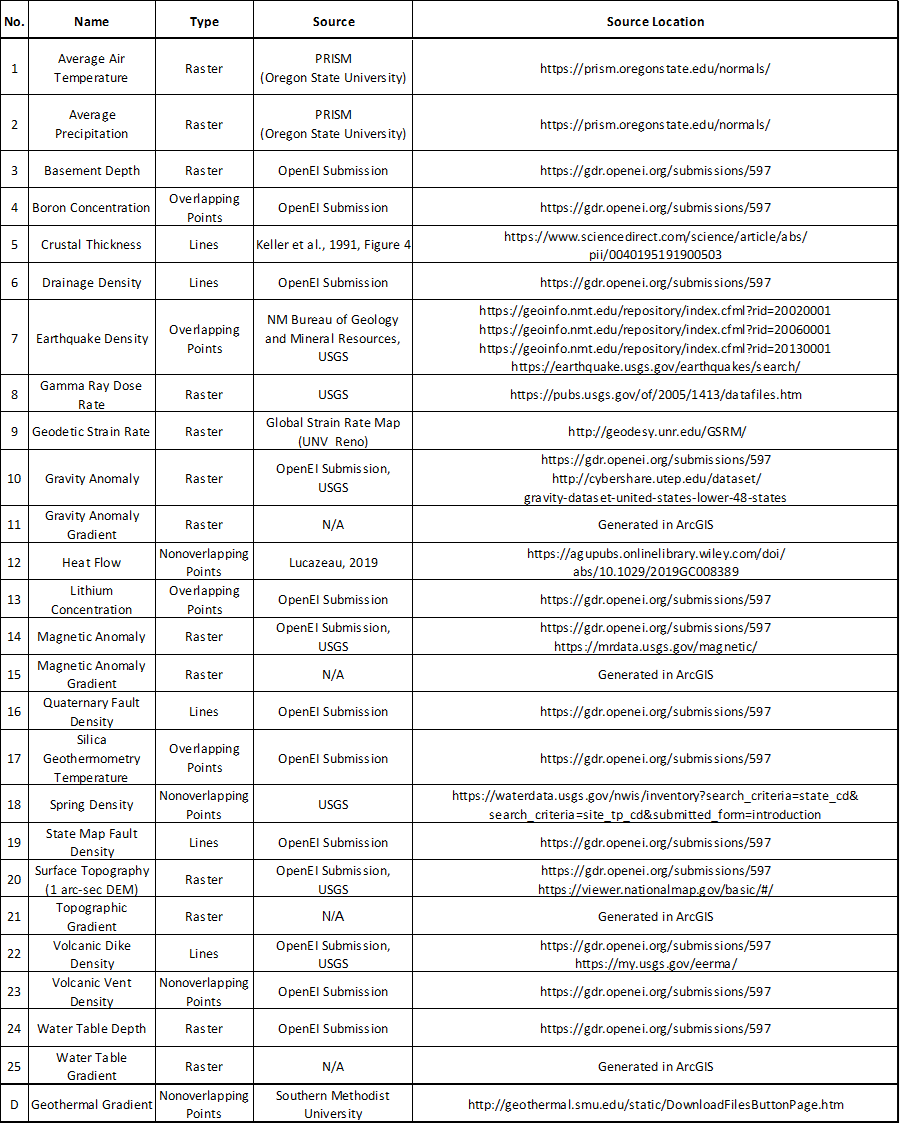
\includegraphics[scale=1]{Table-Features.png}
\caption[Features considered in this the exploration analytics study]{List of data sets considered in this study. Data type, provider, and source location are listed. Numbered features are treated as independent variables. 'D' indicates the dependent variable.}
\label{tab:features}
\end{table}

As discussed in Section \ref{ch2:sysfund}, geothermal systems require permeability, heat, subsurface fluids, a trapping mechanism, and recharge. Following the slightly more simplified PFA assumptions of \citeauthor{bielicki_hydrogeolgic_2015} (\citeyear{bielicki_hydrogeolgic_2015}), an explorationist will want to quickly identify where heat, permeability, and fluids together define a favorable setting for a geothermal prospect. The prepared independent data inputs collectively address all three elements as noted in Table xx. Rather than defining a dependent (predicted) variable that describes a total favorability score, this thesis focuses on a proof of concept prediction for a measurable quantity addressing just the heat risk element: geothermal gradient. This choice was made because a) geothermal gradient provides a direct proxy for accessible heat content, b) gradient point data is available from suitable compilations of well measurements collected across the study area, and c) for EGS applications, the only risk element that must be naturally present is heat. Heat flow might be a reasonable alternative dependent variable, however point values for heat flow in the available well database were derived directly from geothermal gradient values. Geothermometer measurements also suggest resource temperatures, but the uncertainty in fluid pathways leading to the sample location means these values suffer from less spatial and depth certainty than geothermal gradient.

Regarding the remaining two risk elements: direct measurements of permeability (i.e., from downhole logs or core analysis) or fluids (e.g., flow rate from well tests) can be separately predicted using the same methods described in this study. A final favorability score, which is less straight-forward to calibrate for model validation and verification, could potentially be derived from the combined predictions as done in PFA risk assessments. This suggestion is outside of the scope of this thesis and thus appears in the list of future work opportunities (see Chapter 9).

\section{Exploration Data Preparation}

In order to experiment with a variety of machine learning methods, all input data sets first need to be transformed into fully-complete \acrlong{gis} (\acrshort{gis}) layers such that any point on the map of the study area has a corresponding set of 25 independent feature values. Steps taken to condition, process, and otherwise prepare each layer are outlined later in this chapter. As a preface, the following section reviews several key algorithms and concepts applied to one or more of the layers for clarity and reproducibility.

\subsection{Data Preparation Algorithms}

\subsubsection{Extents}

Large data sets imported into ArcGIS or Python for feature preparation required cropping to the southwest New Mexico study area. Two polygons were used for this purpose:

\begin{itemize}
\item Extent Polygon: this is a simple rectangular polygon capturing the broader southwestern NM region. It is defined by the following corner points in degrees N Latitude and degrees E Longitude: \\ (-31.3, -109.1), (31.3, -105.9), (35.4, -105.9), (31.3, -109.1)
\item \acrlong{aoi} (\acrshort{aoi}): this polygon appears in most map figures in this thesis and is the perimeter outlining the nine counties in Southwest New Mexico: Cibola, Valencia, Catron, Socorro, Grant, Sierra, Luna, Dona Ana, and Hidalgo.
\end{itemize}

\subsubsection{Fishnet Points}\label{ssn:fishnet}

\subsubsection{Simple Kriging}\label{ssn:kriging}

\subsubsection{Empirical Bayes Kriging}\label{ssn:ebk}

\subsubsection{Splines}

\subsubsection{Topo to Raster?}

\subsubsection{\acrlong{kde} (\acrshort{kde})}\label{ssn:kde}

\subsection{Data Layers}

\subsubsection{Average Air Temperature}

The University of Oregon PRISM Climate Group hosts regularly-updated spatial data sets of climate-related observations captured from different monitoring networks, including 30-year normals that describe average monthly or annual conditions \citep{daly_physiographically_2008, prism_prism_2021}. 800 m or 4 km resolution grids can be accessed directly from the website. The 800 m resolution air temperature grid was downloaded and imported into ArcGIS, then cropped using the Extent Polygon (Figure \ref{fig:feat_airtemp}). The layer required no further processing.

\begin{figure}[!htp]
\centering
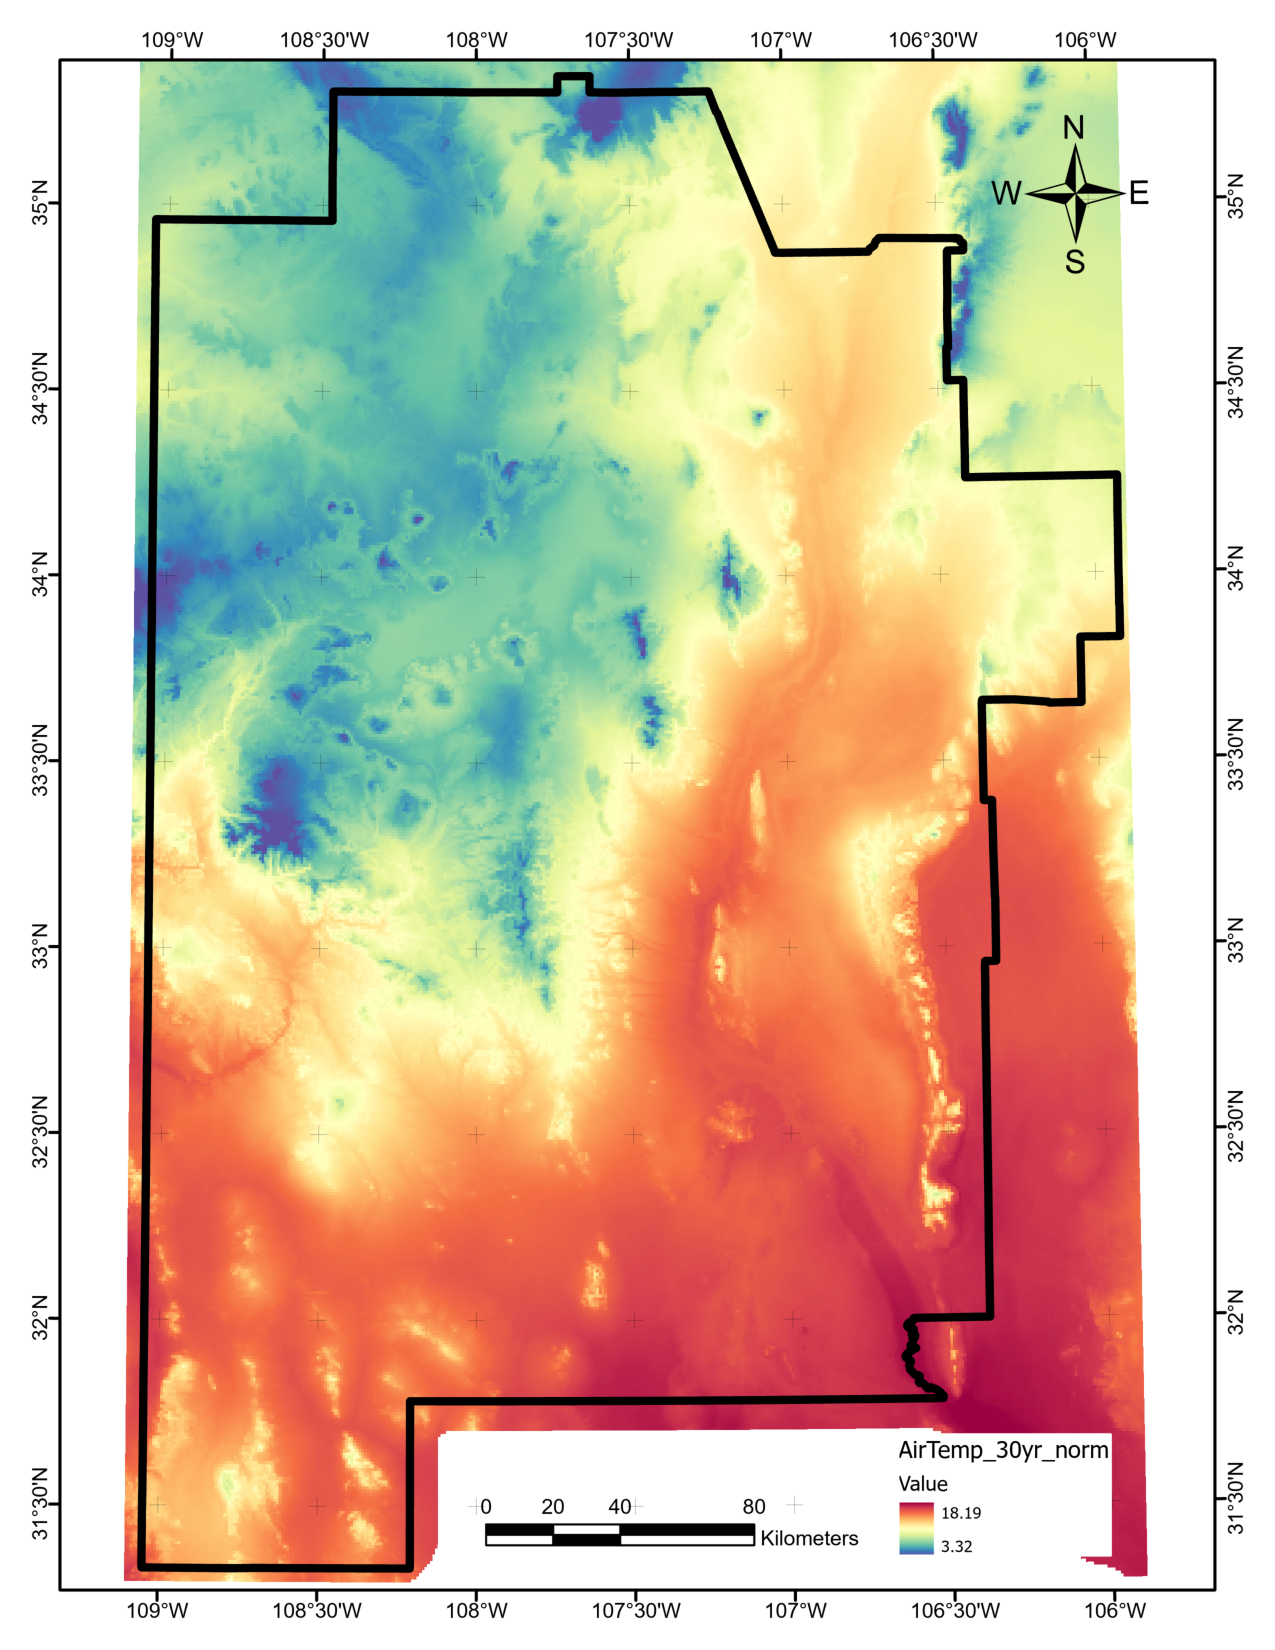
\includegraphics[scale=.6]{Figure-AvgAirTemp}
\caption[Average air temperature data layer]{Average air temperature data layer. Units are degrees Celsius. Data retrieved from \protect\citep{prism_prism_2021}.}
\label{fig:feat_airtemp}
\end{figure}

\subsubsection{Average Precipitation}

The University of Oregon PRISM Climate Group also compiles 30-year normals for average precipitation \citep{daly_physiographically_2008, prism_prism_2021}. The 800 m resolution precipitation grid was downloaded and imported into ArcGIS, then cropped to the Extent Polygon boundaries (Figure \ref{fig:feat_precip}). The layer required no further processing.

\begin{figure}[!htp]
\centering
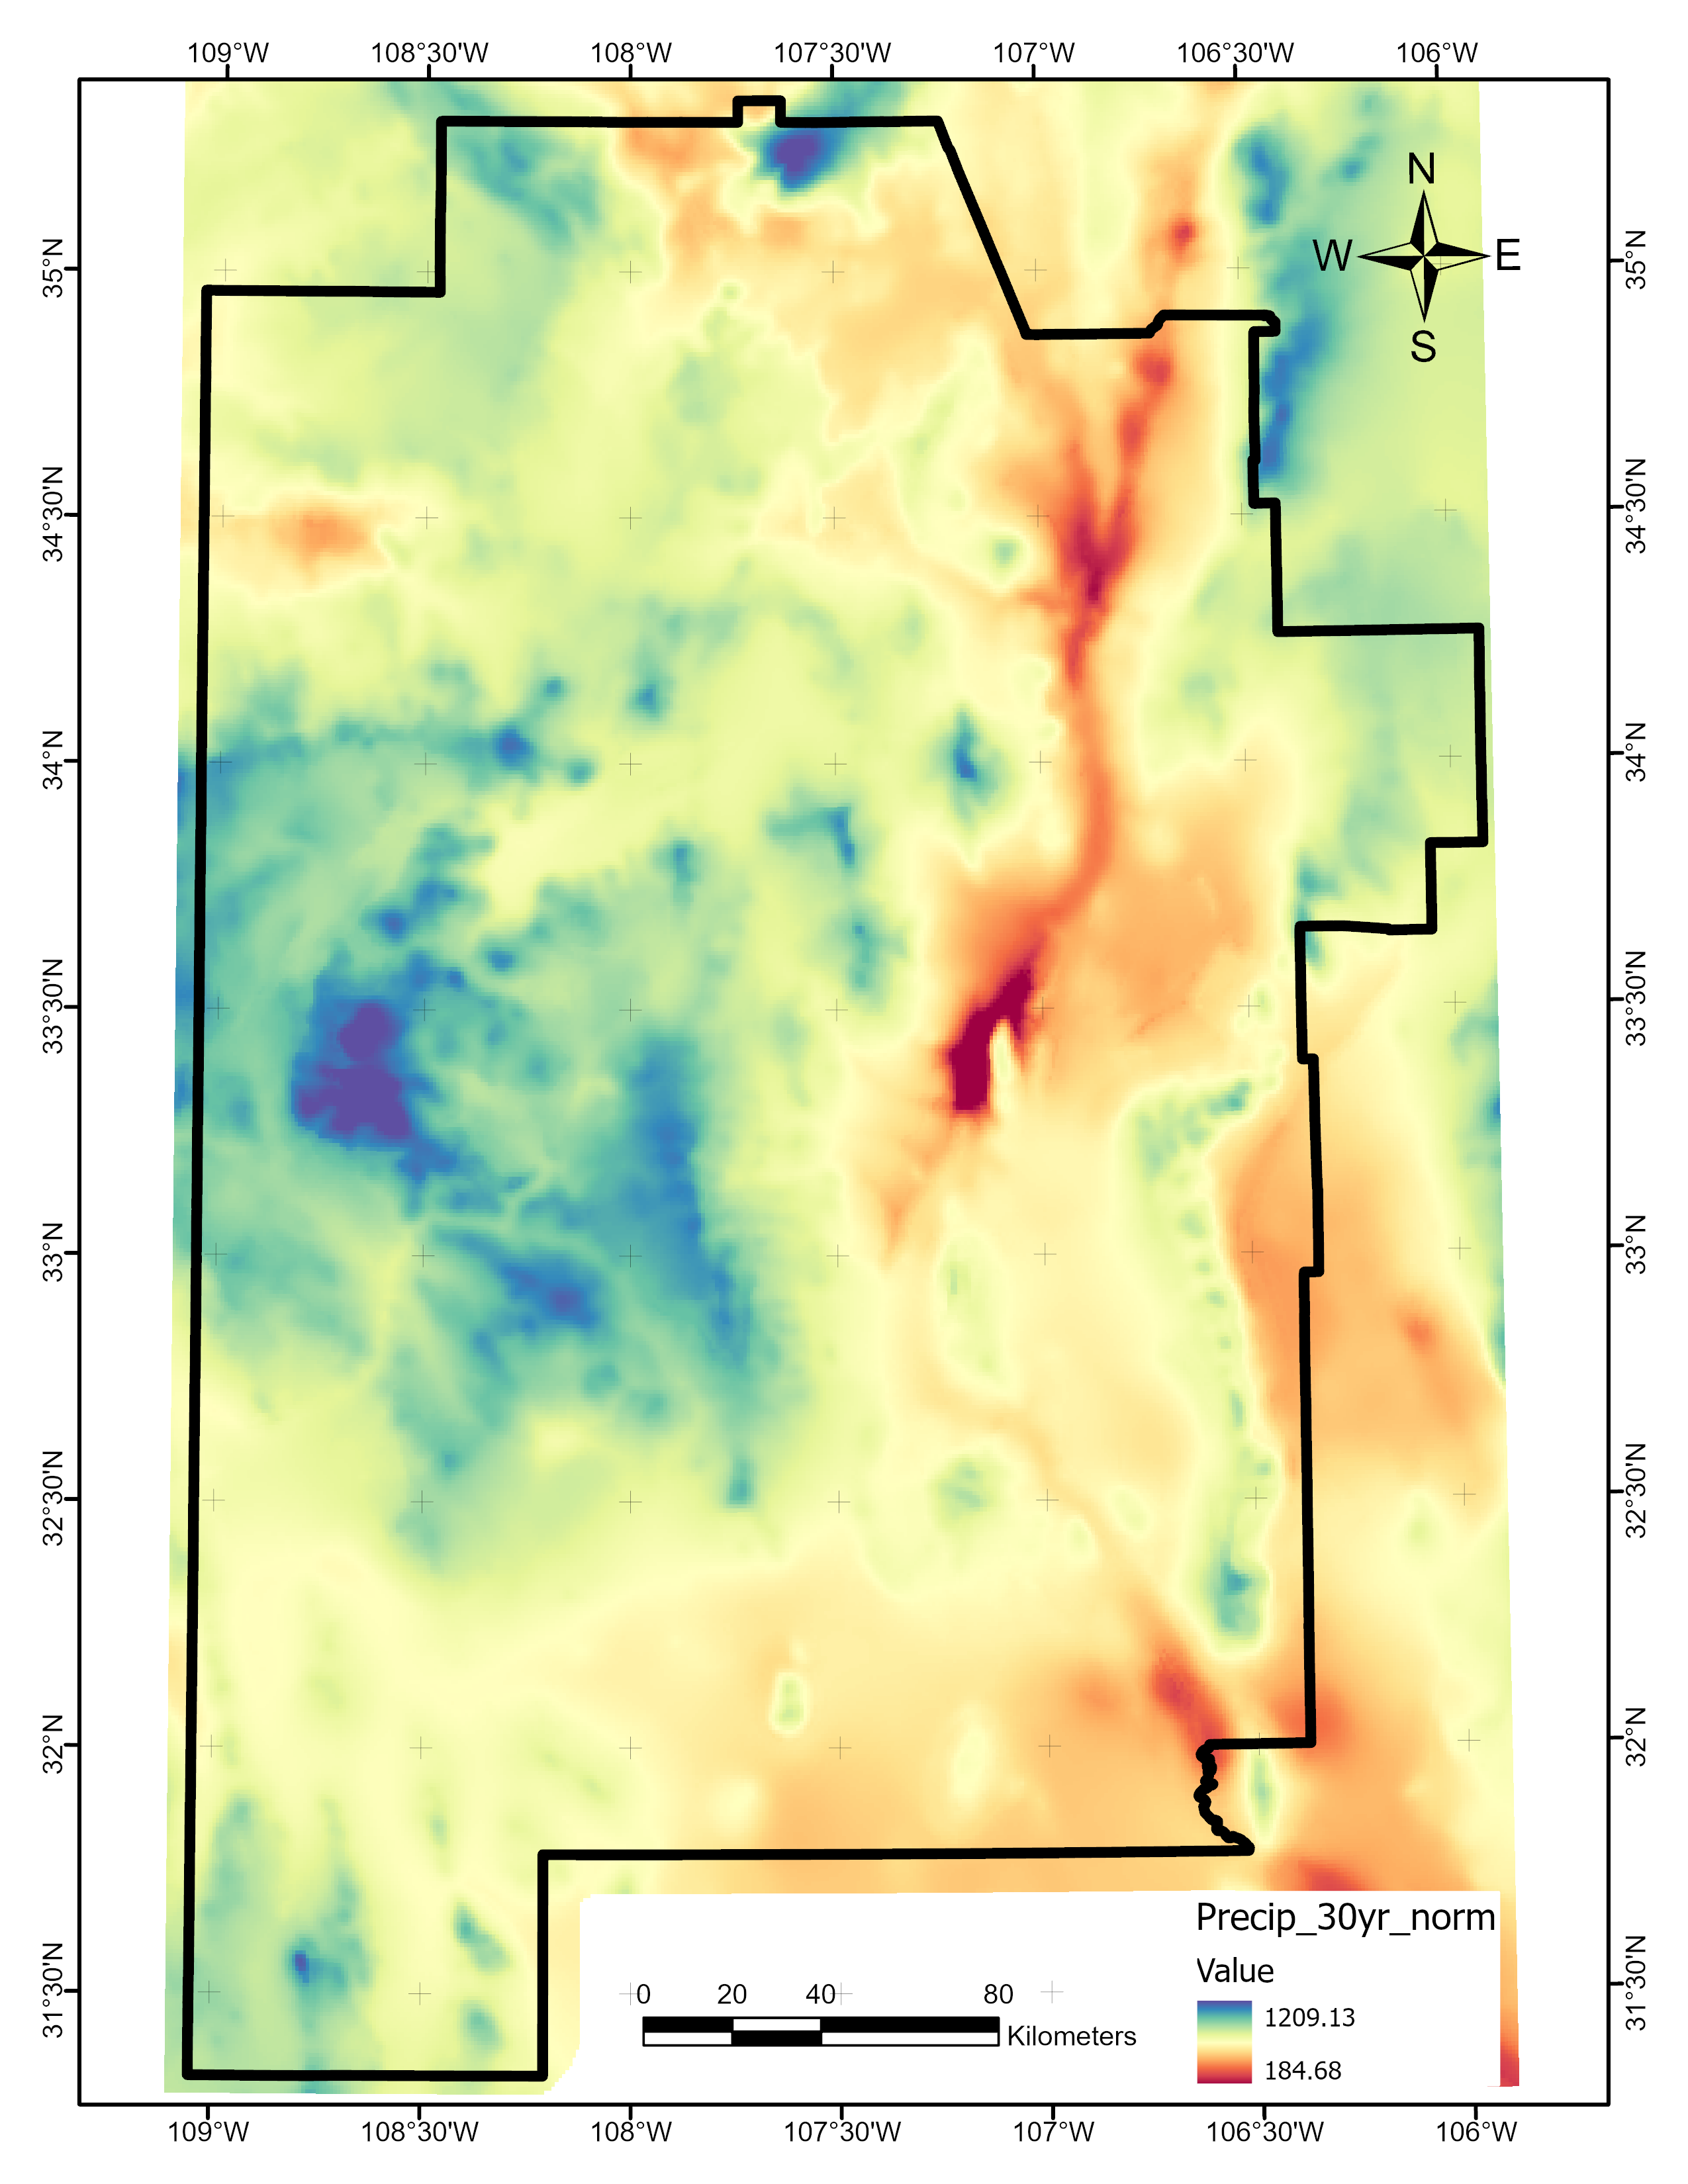
\includegraphics[scale=.6]{Figure-AvgPrecip}
\caption[Average precipitation data layer]{Average precipitation data layer in 800 m resolution. Units are millimeters. Data retrieved from \protect\citep{prism_prism_2021}.}
\label{fig:feat_precip}
\end{figure}

\subsubsection{Basement Depth}

Following the procedure of \citeauthor{pepin_new_2018} (\citeyear{pepin_new_2018}), the basement elevation raster generated by \citeauthor{bielicki_hydrogeolgic_2015} (\citeyear{bielicki_hydrogeolgic_2015}) was downloaded, imported into ArcGIS, and processed to calculate depths. Specifically, a unit conversion from feet to meters was applied. Then, values were extracted on the point fishnet (see \ref{ssn:fishnet}), which highlighted missing data patches in the data. The ArcGIS \textit{Kriging} function interpolated values across these patches using the Ordinary method with Spherical semivariogram, a lag size of 0.096969 automatically determined by ArcGIS, and a variable search radius with a 4-point requirement. Basement depths were then calculated by subtracting the interpolated elevation layer from the surface topography (DEM) layer. However, the higher resolution of the DEM layer caused an imprint of detailed surface geomorphologies to appear on the calculated basement depth layer. To correct for this, the DEM layer was low pass filtered using the ArcGIS \textit{Filter} method, which averages a 3x3 neighborhood around each point in the data set. The final basement elevation layer (Figugre \ref{fig:feat_basementdepth}) was generated from the difference between the low-pass filtered DEM and the kriged basement depth.

\begin{figure}[h!]
\centering
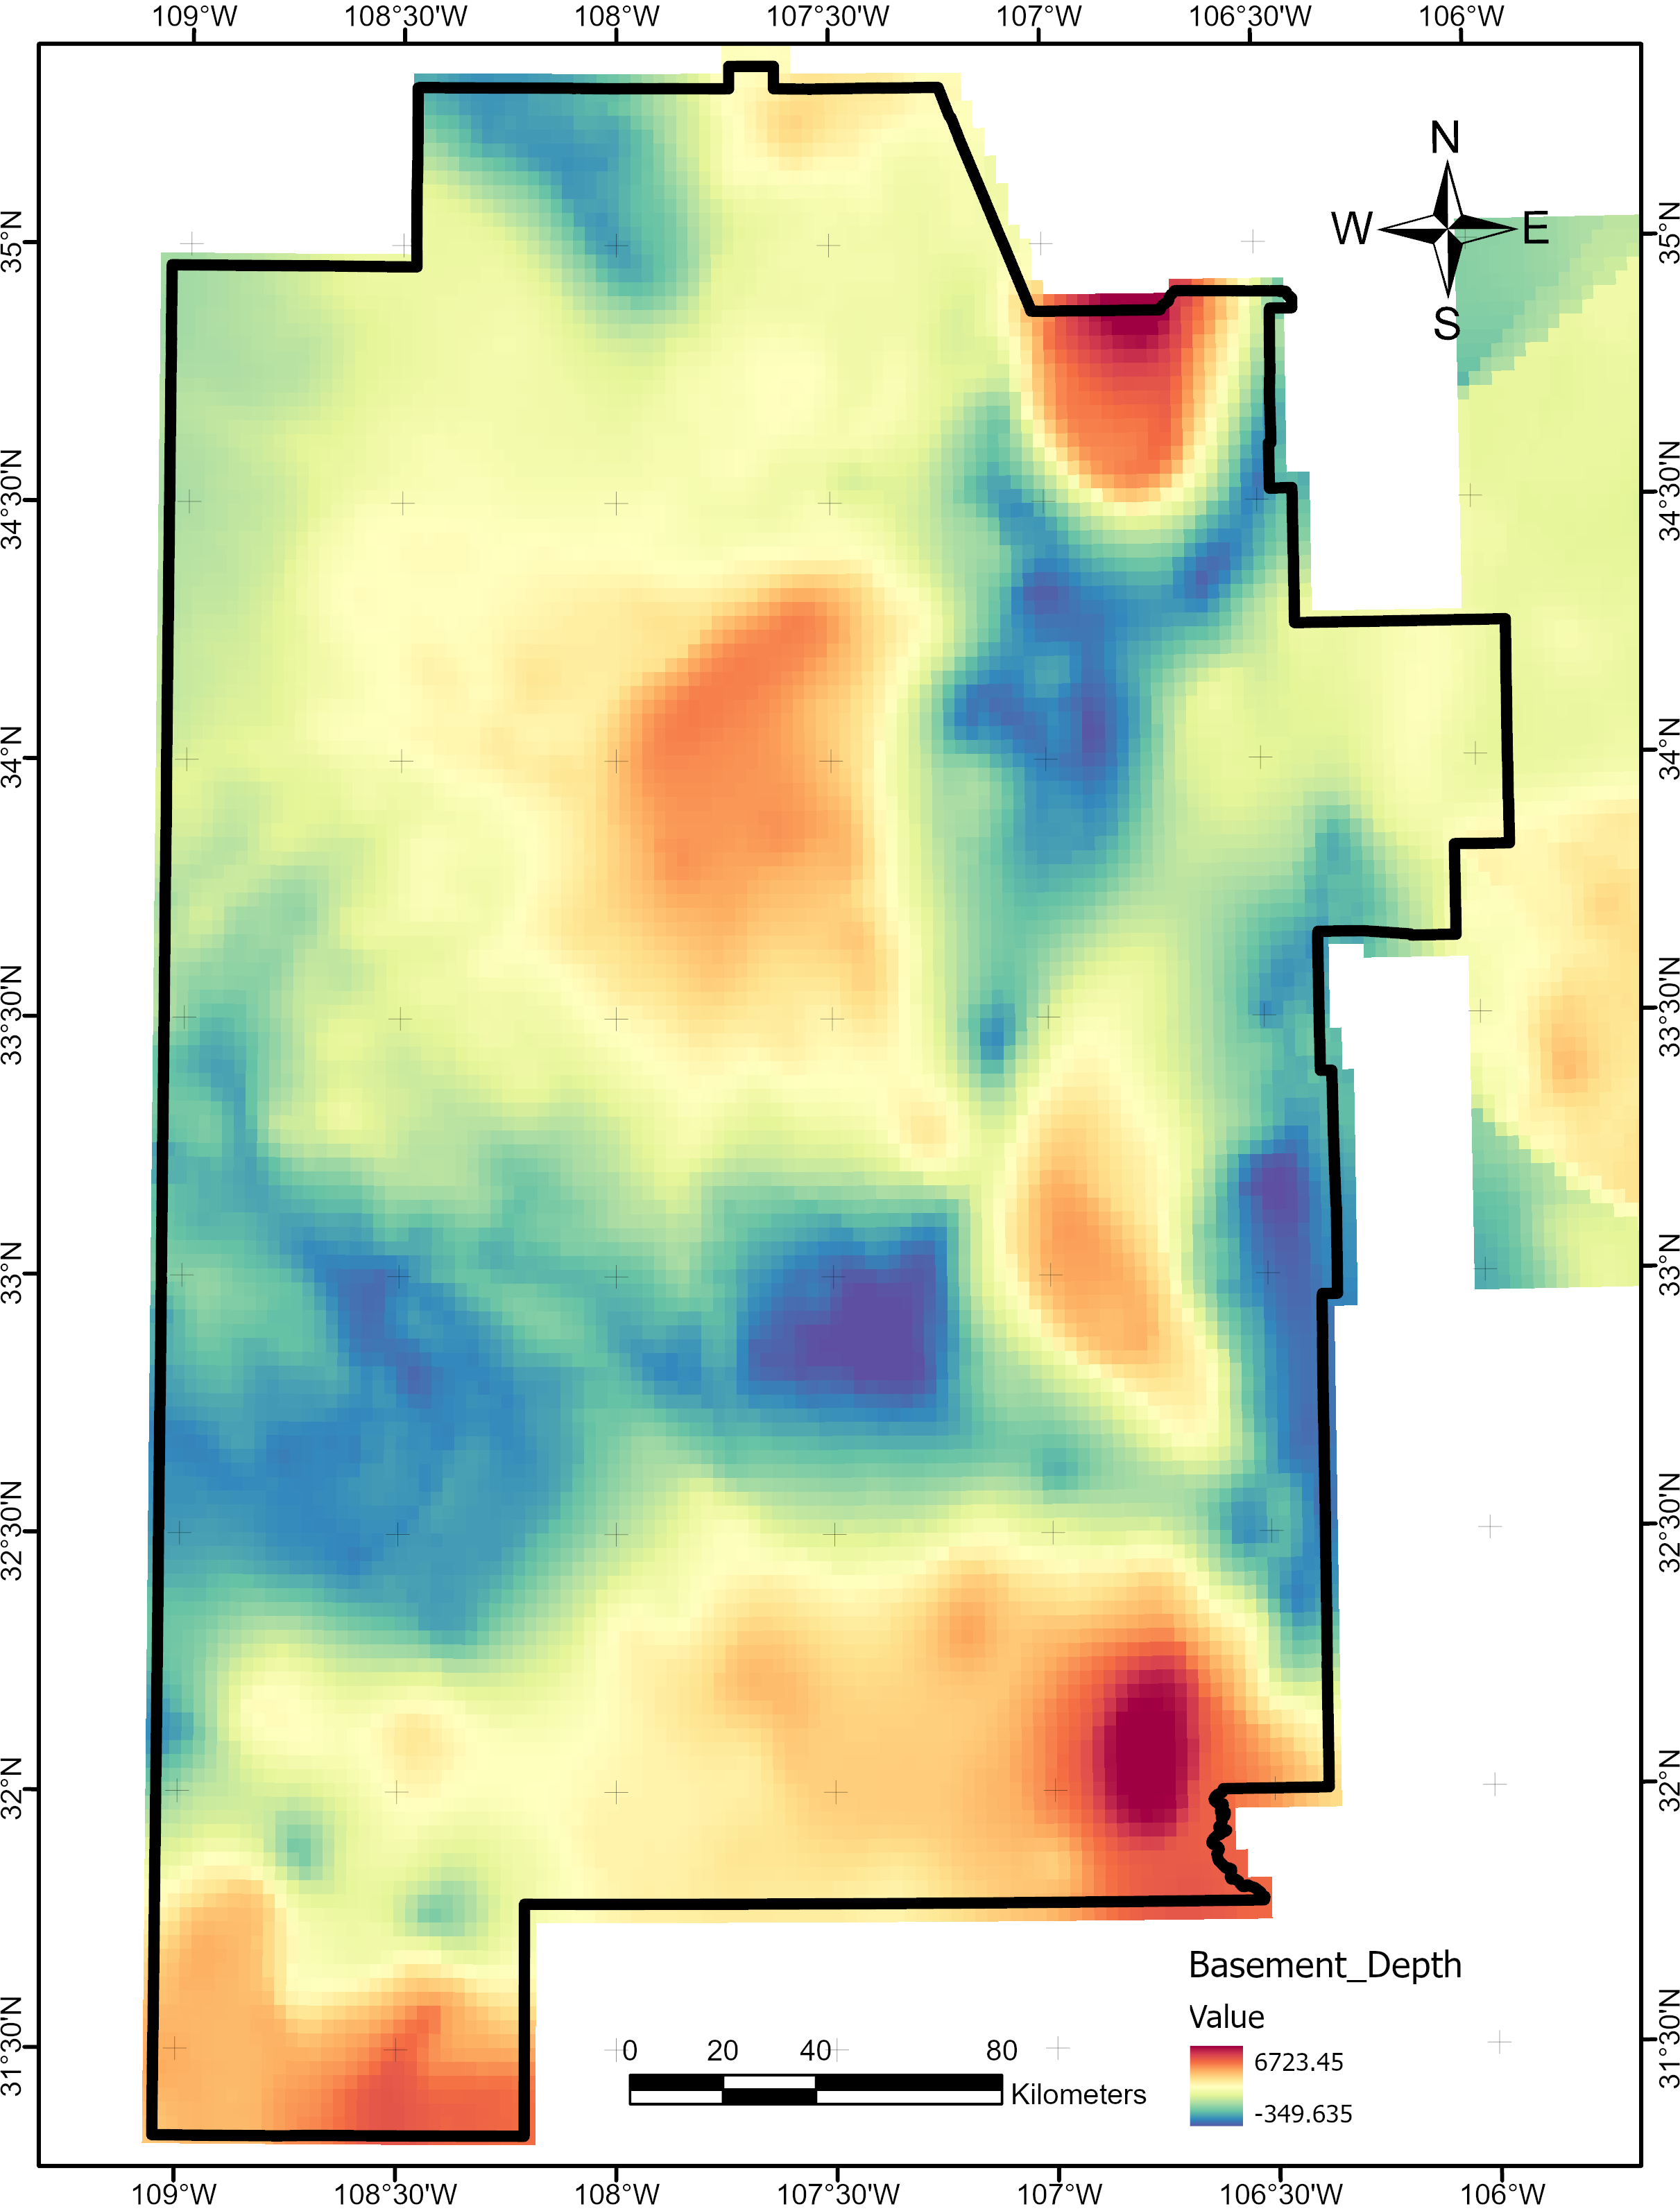
\includegraphics[scale=.6]{Figure-BasementDepth}
\caption[Basement depth data layer]{Basement depth data layer. Units are meters. Layer based on basement elevation raster from \protect\citep{bielicki_hydrogeolgic_2015}.}
\label{fig:feat_basementdepth}
\end{figure}

\subsubsection{Boron Concentration}

Measurements of boron concentration were originally assembled by \citeauthor{bielicki_hydrogeolgic_2015} (\citeyear{bielicki_hydrogeolgic_2015}) from nine sources ranging from USGS records to student dissertations. These data were downloaded from the OpenEI submission \citep{kelley_geothermal_2015} and imported into ArcGIS, then merged into a single dataframe of 5686 measurements within the broader Extent Polygon bounds to avoid edge effects within the AOI. The inconsistent spatial distribution of the data and sometimes significant variation among overlapping values from different measurement years created a unique challenge for making a representative GIS layer to use for analysis. An initial attempt to fit and interpolate the data using tuned Gaussian Process models created feature layers with too much local structure and little character away from the input data points. The ArcGIS \textit{Empirical Bayes Kriging} routine was selected instead due to its unique characteristics. For the final layer (Figure \ref{fig:feat_boron}), EBK was applied with the Empirical data transformation type, a maximum of 100 points in each local model, 100 simulated semivariograms with K-Bessel model type, and a standard circular search neighborhood with a radius of 1.1957 (auto-generated), minimum of 10 neighbors, and maximum of 15 neighbors. The output grid cell size was set to 0.01 degrees. Of important note: the calculation option to include all coincident data was selected, so all overlapping measurements were considered in generating the final layer.

\begin{figure}[h!]
\centering
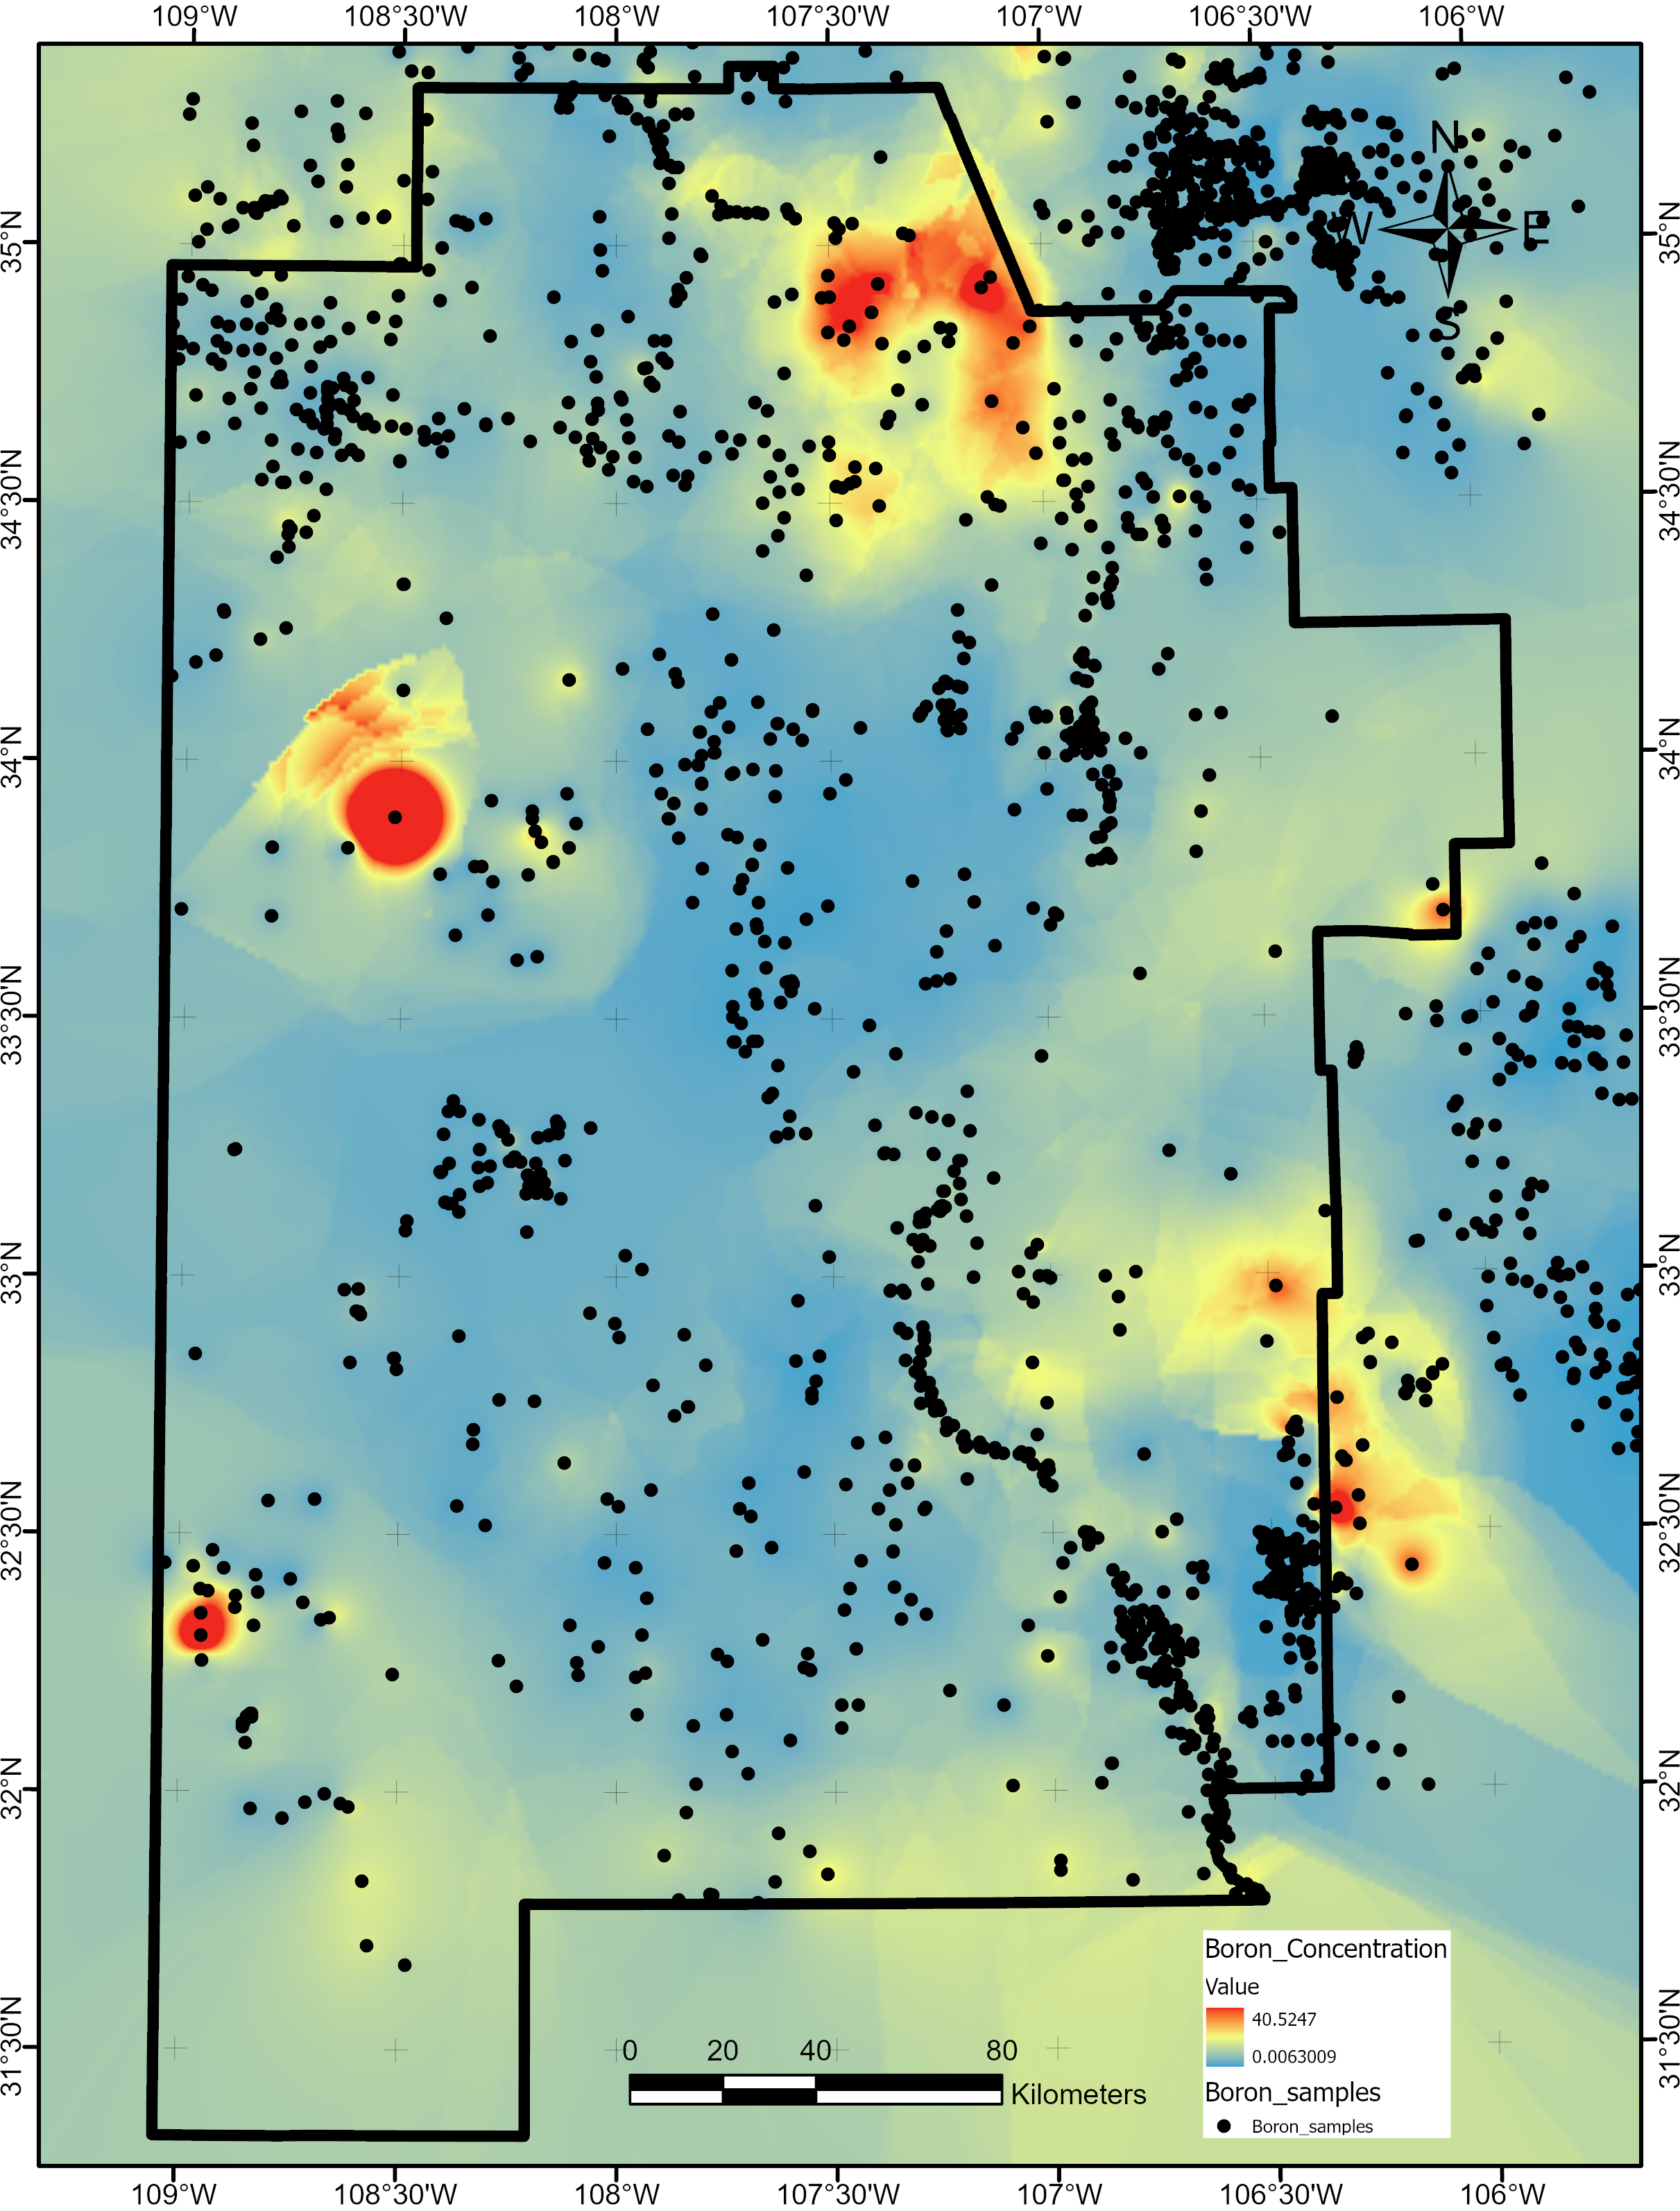
\includegraphics[scale=.6]{Figure-Boron}
\caption[Boron concentration data layer]{Boron concentration data layer. Units in ppm or mg/L. Black dots indicate sample locations in complete data set from \protect\citep{bielicki_hydrogeolgic_2015}.}
\label{fig:feat_boron}
\end{figure}

\subsubsection{Crustal Thickness}

In the absence of a recent 3D seismic survey constraining crustal thickness in the study area, the 2.5D regional map published by \citeauthor{keller_comparative_1991} (\citeyear{keller_comparative_1991}) was used for the crustal thickness feature layer. Similar to the procedure described in \citep{pepin_new_2018}, the Keller map was georeferenced in ArcGIS, and thickness contours were manually digitized as polylines. These polylines continued slightly beyond the AOI boundary to ensure proper constraints for surface creation without artifacts near the AOI edges. The ArcGIS function \textit{Feature to 3D by Attribute} converted the polylines into 3D contours, and \textit{Topo to Raster} generated a continuous final grid (Figure \ref{fig:feat_crust}). Since the Keller map was derived from low-resolution seismic lines from the 1960s-1980s, the result is a very low frequency approximation for crustal thickness variations associated with the CP and RGR. As such, \textit{Topo to Raster} used an output cell size of 0.025 degrees. Other parameters include: margin in the cells of 20, smallest z value for interpolation of 25, largest z value for the interpolation of 55, Enforce selection for drainage enforcement, and maximum iterations of 20.

\begin{figure}[!htp]
\centering
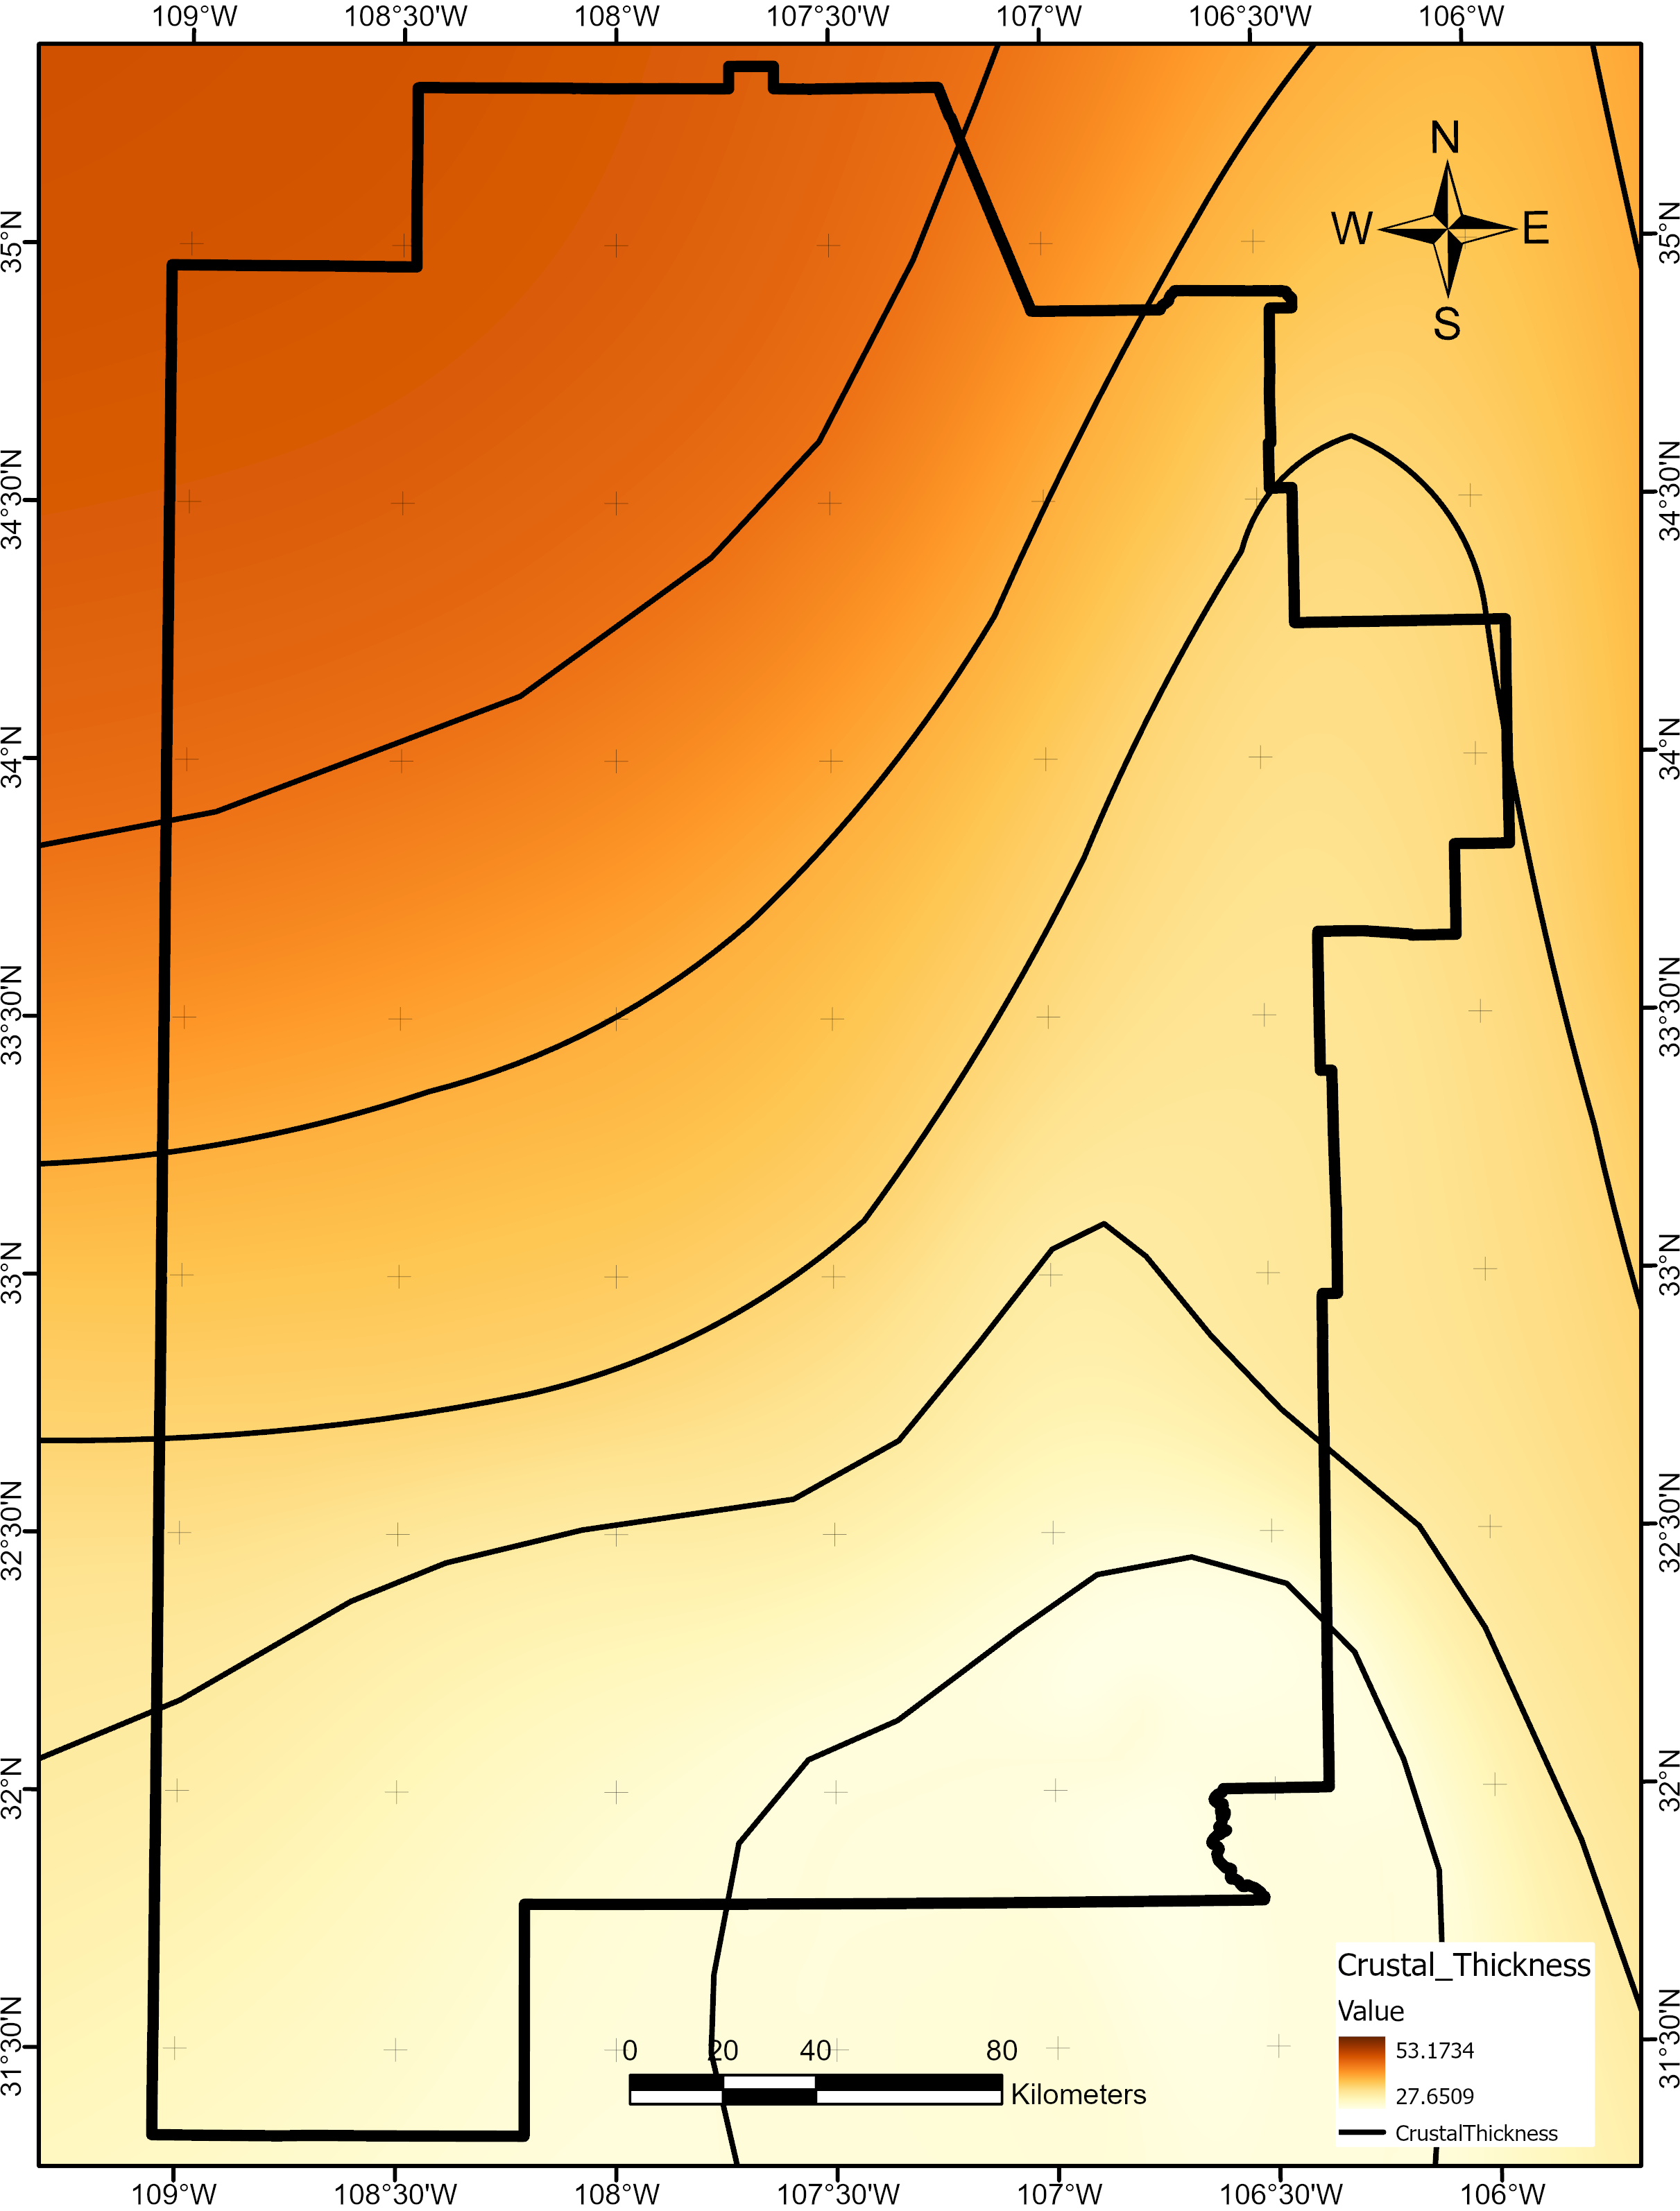
\includegraphics[scale=.6]{Figure-CrustalThickness}
\caption[Crustal thickness data layer]{Crustal thickness data layer. Units in kilometers. Black lines refer to contours digitized from \protect\citep{keller_comparative_1991}.}
\label{fig:feat_crust}
\end{figure}

\chapter{Cost-Modeling for an EGS Power Plant Expansion}\label{ch4:cm_prep}
\section{EGS Expansion Concept}\label{ch4:cm_concept}
\subsection{Lightning Dock EGS}\label{ch4:lightning_dock_egs}
Lightning Dock is presently the only commercial power plant operating in the state of New Mexico (see Section \ref{ch2:lightning_dock}). The net generating capacity after its first phase of development was 4 MW in 2013, with the expectation of upgrading to 10 MW in a second development phase that never came to fruition. Instead, the facility underwent a significant refit in 2018, resulting in a net capacity of 11.2 MW generated entirely from hydrothermal brine production \citep{bonafin_repowering_2019}.

Department of Energy-funded efforts to characterize the geothermal resources of the Animas Valley --- where Lightning Dock is located --- revealed the presence of two different thermal reservoirs: the hydrothermal resource targeted by Lightning Dock where deep geothermal fluids ascend along the Animas Valley Fault complex to $\approx$365-1000 m depth, and a secondary interval at $\approx$900-1200 m depth that requires permeability enhancement for production \citep{schochet_development_2001}. The Horquilla limestone formation defines the second reservoir, estimated to span a minimum volume of 6 cubic km based on conservative figures. By one proprietary study completed in 2001 for Ormat Technologies, a commercial geothermal company, the Horquilla has a 88\% probability of 6 MW in recoverable electricity generation potential \citep{schochet_development_2001}.

\citet{schochet_development_2001} proposed the construction of a 6 MW hybrid power plant combining hydrothermal and EGS-sourced power generation a decade before operations commenced at Lightning Dock. In their development plan, they noted several benefits of pursuing EGS in this location:
\begin{itemize}[itemsep=2pt]\label{ch4:ld_egs_support}
    \item Relatively shallow resource drives lower drilling costs
    \item EGS water requirements are attainable from paired hydrothermal operations
    \item A comprehensive initial assessment determined no significant environmental degradation is expected from geothermal operations
    \item Lightning Dock has direct access to in-place transmission lines  
    \item Opportunities exist for electricity sales to local users
    \item Purchase agreements with regional utilities are incentivized by NM legislation
\end{itemize}

As suggested by this list, the conditions at Lightning Dock offer a nearly ideal test case for an EGS proof of concept on a manageable scale. Historical land utilization in the area is primarily agricultural with few residences, so risk is low for any adverse impact on an existing population. In addition, use of a binary cycle design as proposed by \citet{schochet_development_2001} offers the potential for power production with zero greenhouse gas emissions.  

In this thesis, the \citeauthor{schochet_development_2001} concept is revisited with the existing geothermal production at Lightning Dock kept in mind; rather than building a new hybrid facility, the revised concept involves targeting the deeper reservoir as a NF-EGS development with a tie-back to the current Lightning Dock facility. Stepping out from the hydrothermal zone in proximity to the Animas Valley Fault complex, thermal conditions settle to a high background geothermal gradient between $\approx$ 80-120 K/km based on boreholes TG 56-14 and TG 12-7 \citep{cunniff_final_2003} -- certainly high enough to support geothermal capture. These conditions make for an interesting case study on risk mitigation options for EGS production planning.

Public records regarding power generation at Lightning Dock provide some guidance on the appropriate size for an EGS expansion. After phase 1 development, the plant produced 4 MW. An additional 6 MW was slated for phase 2, but re-powering of the plant actually added 7 MW to the capacity after several years of development stasis \citep{think_geoenergy_turboden_2020}. \citeauthor{schochet_development_2001} originally proposed a 6 MW hybrid plant for the site, but they also noted 6 MW from the Horquilla was likely understating the full reservoir potential (\citeyear{schochet_development_2001}). In consideration of the step-wise trajectory of plant improvements and the assessment of available thermal resources, this case study targets 5 MW as a expansion goal. 

\subsection{New Mexico Electricity Demand}\label{ch4:nm_rps}
Pursuing the expansion of a power plant requires sufficient demand to ensure total revenue offsets project expenses. Fortunately, New Mexico regulations support the further development of geothermal power production in the state. Specifically, the Energy Transition Act signed in 2019 updated the New Mexico \acrlong{rps} (\acrshort{rps}) to go zero-carbon by 2050, with milestone targets along the way \citep{lillian_new_2019}. The RPS dates back to the Renewable Energy Act passed in 2004 and comes with several carve-outs, including a 30\% requirement for wind energy, 20\% for solar, and 5\% for other renewables like geothermal \citep{dsire_dsire_2021}. Public Service Company of New Mexico (PNM) is the state’s largest energy provider and services the Lordsburg area where Lightning Dock is located. PNM and Cyrq Energy currently share a 20-year \acrlong{ppa} (\acrshort{ppa}) for electricity generated at Lightning Dock. The PPA has gone through amendments over time to update both the wattage supplied to PNM and the pricing structure per MWh \citep[e.g.,][]{pnm_public_2014,stanfield_new_2017}. This indicates a PPA can be revisited if conditions change, which is an important aspect to consider when modeling project financials. 
In addition to the RPS requirement for a diversified renewables portfolio, coal power plants across the state face mandated shut-downs as a consequence off the Energy Transition Act. Coal currently supplies a large fraction ($\approx$ 45\%) of electric power sector consumption in New Mexico (Figure \ref{fig:nm_energy_consumption}). The supply gap introduced as coal-based production ramps down to zero could more than compensate for a 5 MW addition of no-emissions energy to the New Mexico grid.

\begin{figure}[!htp]
\centering
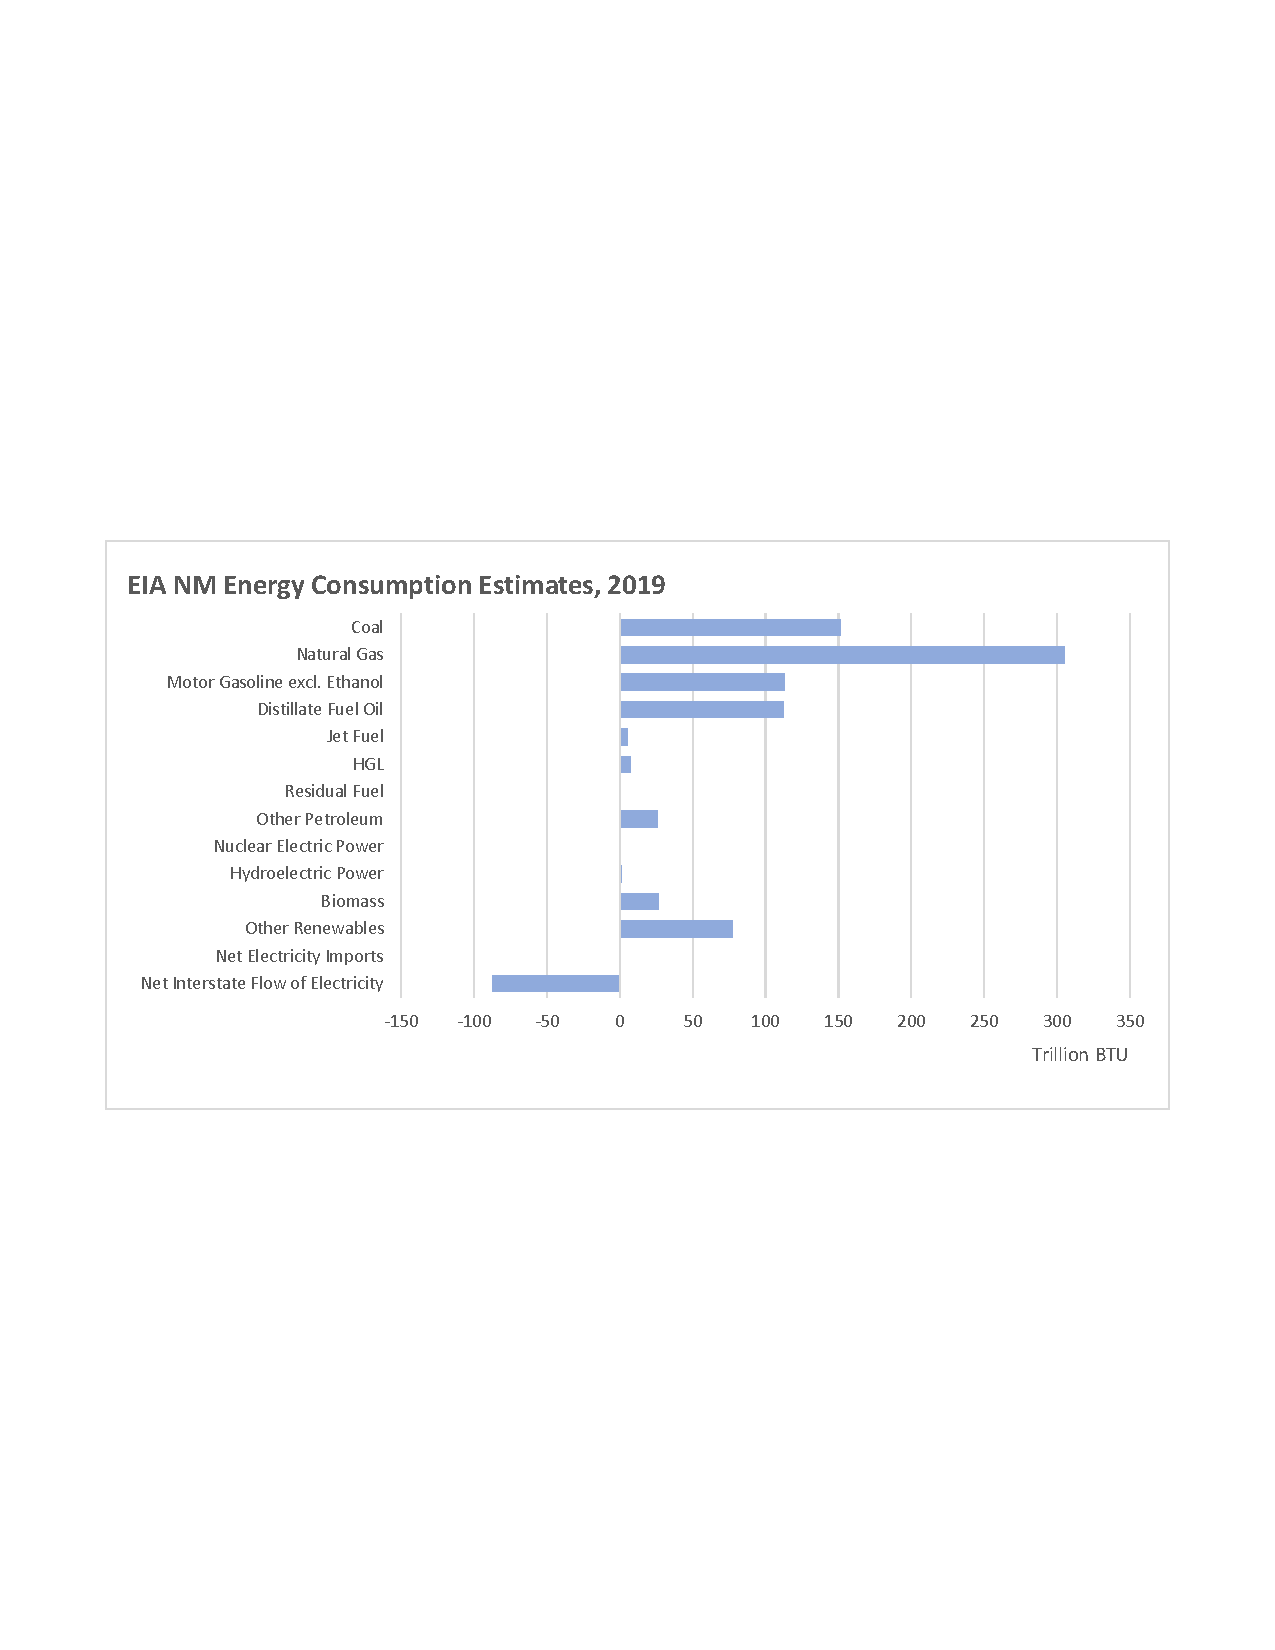
\includegraphics[width=\textwidth]{templates/images/Figure-EIA_NM_Energy_Consumption.pdf}
\caption[NM energy consumption]{Energy consumption by source for New Mexico. Adapted from data and graphics reported by the EIA \protect\citep{eia_new_2021}.}
\label{fig:nm_energy_consumption}
\end{figure}

\subsection{Modular Geothermal}\label{ch4:modular_geothermal}
Limiting this expansion to a single 5 MW facility represents one design alternative, but others exist as well. One flexible option uses modular technology that recently captured the attention of high-stakes investors across the world \citep{shieber_bill_2019}. Climeon has engineered a compact binary cycle unit capable of 150 kW of generated electricity using inlet fluid temperatures rated up to 120℃ and flow rates of up to 35 kg/s \citep{climeon_climeon_2021-1}. These units can be combined into a larger deployable Power Block for 1050 kW of generated electricity \citep{winther_power_2018} (Figure \ref{fig:climeon_powerblock}). Using this technology, power plants can now be treated like multi-unit assemblages, installed all at once or over an extended period of time based on operator needs \citep{climeon_why_2018}.

\begin{figure}[!htp]
\centering
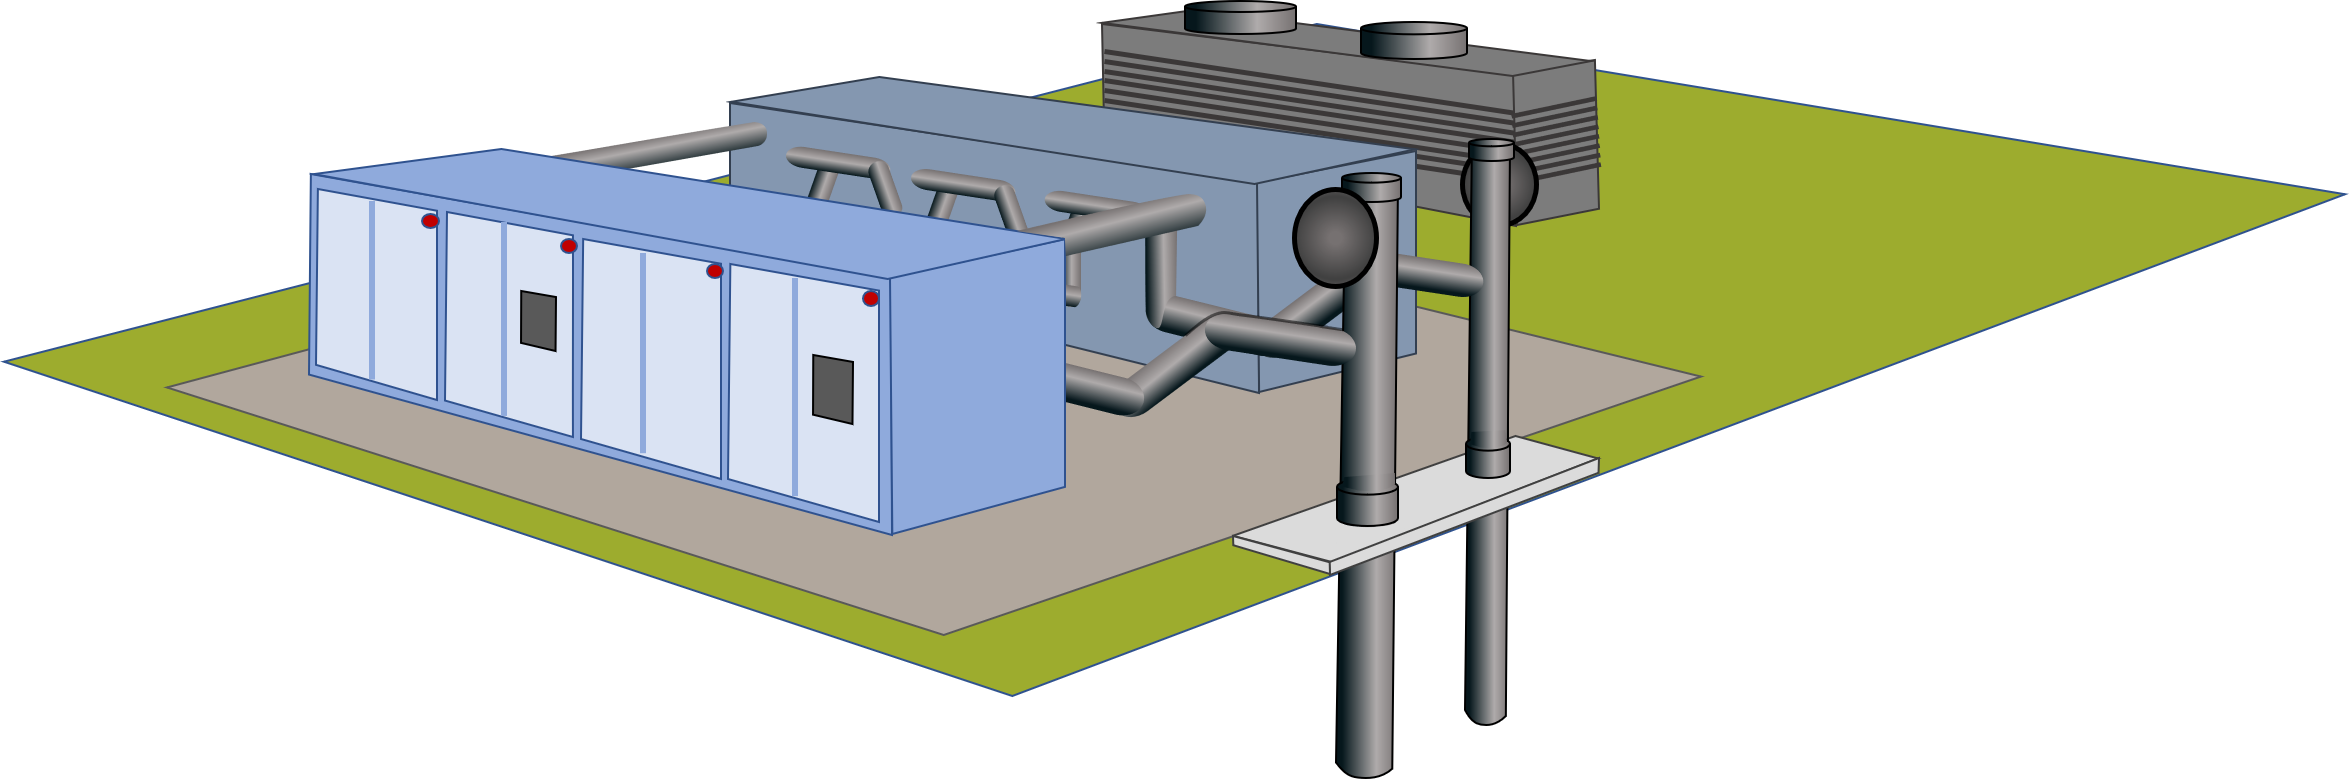
\includegraphics[width=\textwidth]{templates/images/Figure-Climeon-PowerBlock.png}
\caption[Modular power plant schematic]{Modular binary cycle power plant concept, adapted from Climeon PowerBlock schematic diagram \protect\citep{climeon_climeon_2021-1}. Each block consists of seven active units chained together for $\approx$1 MW of generating capacity.}
\label{fig:climeon_powerblock}
\end{figure}

\subsection{Flexible Cost Models}\label{ch4:flex_models}
As discussed in Section \ref{ch2:cost_models}, cost models can provide insights into the potential value gained or lost by a proposed facility before construction even begins. Well-established geothermal cost models like GETEM \citep{entingh_volume_2006} present a highly parameterized but deterministic view of cost and investment opportunity given a defined geothermal resource and development concept. Other models may apply different assumptions or mathematical treatments for various facets of the system, however they uniformly offer a single-track aspect to how the project unfolds over its lifecycle. Users can test ideas, but the solution space remains under-explored due to implicit assumptions of variable trends or static behaviors for a highly-dynamic system.

In the cost model outlined below, the economic analysis incorporates uncertainty by replacing single value estimates with distributions for model variables. This enables the model to produce a representative range of possible outcomes when simulated many times over. In addition, the model flexibly adapts by executing design options, where model updates triggered by changing conditions allow the system to realize upside potential or characterize the extent of downside risk. Designs need not be static, and flexibilities can greatly increase the expected value of a project by exploring execution strategies otherwise missed by more traditional modeling approaches \citep[Chapter 6]{de_neufville_flexibility_2011}.

\section{Static Cost Model}\label{ch4:cm_structure}
Geothermal cost models typically report Levelized Cost of Electricity (LCOE) for simple comparison with other renewable energy sources. However, LCOE is standardized to represent the total lifetime costs incurred by a power plant normalized by the total power generation from start-up to plant decommissioning. LCOE is thus not well-suited for communicating projected gains or losses under different plant designs or scenarios, which are the focus of this analysis. Instead, the model described here relies on \acrlong{npv} (\acrshort{npv}), a simple measure of project worth that accounts for the time value of money by applying a single interest rate, the discount rate, for both borrowing and deposits \citep[p.\ 195-215]{de_neufville_flexibility_2011}. Here, ``present value'' refers to a 2020 cost basis. For power generation over a 30-year lifespan -- the default for geothermal models like GETEM \citep{entingh_volume_2006} -- this basis takes the model out to 2050, a common benchmark year for future projections. 

\subsection{NPV Model}\label{ch4:cm_npv}
Following the general outline for geothermal cost modeling from previous work \citep[e.g.,][]{augustine_hydrothermal_2009, beckers_introducing_2013,tester_future_2006}, this thesis considers revenue (R), operating \& maintenance costs (OPEX or OM), and capital expenditures (CAPEX or C) as the primary components defining annual cash flow (see Equation \ref{eq:cm_components}). Capital expenses can be further decomposed into five  sub-components associated with exploration, drilling \& completions, reservoir stimulation, fluid distribution, and power plant costs. Likewise, operating expenses subdivide into subsidiary costs for the power plant, wells, and water management.
\begin{equation}
    \label{eq:cm_components}
    \begin{aligned}
    NPV &= \sum_{t=1}^{T}D_t \cdot \left( R_t - C_t - OM_t \right)\\
    \text{where:}\\
    C_t &= \left[C_{expl} + C_{dc} + C_{stim} + C_{dist} + C_{pp}\right]_t\\
    OM_t &= \left[OM_{pp} + OM_{well} + OM_{water}\right]_t
    \end{aligned}
\end{equation}
\\
Revenue and expenses are treated on an annual basis, meaning shorter-term fluctuations like price and production seasonality are not explicitly modeled. $D_t$ in Equation \ref{eq:cm_components} defines the time-based conversion factor between cash flow for a specific year and discounted cash flow for the basis year (see Equation \ref{eq:discount_rate}).

\subsubsection{Revenue}\label{ch4:cm_rev}
Calculations of undiscounted revenue require an estimate of the electricity produced within a year ($W$) and the price set by a power purchase agreement ($p_{PPA}$) for that electricity \citep{entingh_volume_2006}. 

\begin{equation}
    \label{eq:cm_rev}
    R = W \cdot p_{PPA} = (b_e \cdot \dot{m}) \cdot p_{PPA}
\end{equation}
Brine effectiveness ($b_e$) describes the electricity output per unit flow of produced brine ($\dot{m}$) and depends on the production temperature of the brine. The GETEM model uses an empirical correlation between the brine temperature ($^\circ$C) and effectiveness (w-hr/kg) \citep[p.\ 62]{entingh_volume_2006}:

\begin{equation}
\begin{aligned}
    \label{eq:brine_eff}
    b_e &= C_0 + C_1 \cdot T_{prod} + C_2 \cdot T_{prod}^2 + C_3 \cdot T_{prod}^3 + C_4 \cdot T_{prod}^4 \\
    &\quad C_0 = 9.41376 \\
    &\quad C_1 = -0.182542 \\
    &\quad C_2 = 0.0001765735 \\
    &\quad C_3 = 0.000012204486 \\
    &\quad C_4 = -0.0000000335559
\end{aligned}
\end{equation}

In the GETEM interface, a user chooses either to determine the electricity output for a specified input temperature and flow rate, or alternatively, derive the required flow rate to meet a pre-determined power sales capacity at the same input fluid temperature \citep{entingh_volume_2006}. Since the Climeon analog has a known net capacity of 150 kW per unit or 1.05 MW for each PowerBlock, and standard flow rates are provided in models like GETEM, both options are explored in this thesis.

\subsubsection{Exploration Capital Expenses}\label{ch4:cm_capex_expl}
Costs for exploration activities are estimated by the same method defined for the 2012 GETEM model (Equation \ref{eq:cm_capex_expl}) \citep{eere_getem_2012}. 

\begin{equation}
\label{eq:cm_capex_expl}
    C_{expl} = PPI \cdot \left[ 1.12 \cdot (\$1\text{M} + 0.6\cdot C_{dc}) \right]
\end{equation}

This relationship assumes slim hole (3-6" diameter) drilling for exploration at a 60\% discounted cost compared to standard-sized ($\geq$ 8.5" diameter) geothermal wells. The constant \$1M term accounts for pre-drilling costs, including field work, geophysical surveys of field structure, and interpretation of results. Technical and office support is covered by an additional 12\% applied to the estimate \citep{eere_getem_2012}. Total exploration costs are converted to a 2020 cost basis using the \acrlong{ppi} (\acrshort{ppi}) for electric power generation from the U.S. Bureau of Labor and Statistics \citep{us_bls_ppi_2021}.

\subsubsection{Drilling \& Completions Capital Expenses} \label{ch4:cm_capex_dc}
Geothermal drilling and completions costs differ from traditional oil \& gas wells due to differences in hole diameter, thermal and geochemical conditions, and the strength and abrasiveness of the target formations \citep{lowry_geovision_2017}. Here, drilling capital expenditures rely on a cost curve described by \citet[Eq. 4,\ ][]{beckers_introducing_2013}.

\begin{equation}
\label{eq:cm_cdc}
    C_{dc} = PPI \cdot \left[ 1.65 \cdot 10^{-5} \cdot \text{MD}^{1.607} \right]
\end{equation}
where $C_{dc}$ is measured in \$M and MD refers to well measured depth in meters. Each power plant module will require an injector-producer pair, so this represents one-half of the drilling cost per module. Drilling costs are converted to a 2020 cost basis using the PPI for electric power generation \citep{us_bls_ppi_2021}. 

Note that Equation \ref{eq:cm_cdc} was derived for well depths of 1600-9000 m. Assuming an average geothermal gradient of 100 K/km (Table \ref{tab:cm_resource_params}), the wells considered for this study could extend slightly shallower than this range, so this should be viewed as a minimum drilling \& completions estimate. The stochastic model considered later in this study includes variability in both geothermal gradient and drilling costs for a more comprehensive treatment of both variables.

\subsubsection{Simulation Capital Expenses}\label{ch4:cm_stim}
EGS at Lightning Dock requires stimulation of the Horquilla reservoir to create fluid pathways for thermal extraction. The stimulation cost estimate used in this study comes from the recent GeoVision analysis \citep{lowry_geovision_2017}:

\begin{equation}
\label{eq:cm_capex_stim}
    C_{stim} = \$1,250,000
\end{equation}

Since this represents a recent ballpark estimate, no cost basis conversion was applied in the model. In fact, the value in Equation \ref{eq:cm_capex_stim} may be high since it includes the cost of water, which may not be a factor at Lightning Dock with the availability of hydrothermal brine from adjacent power plant operations. The model assumes stimulation is only performed for the injection well in each injector-producer pair, so this represents a \textit{per module} value.

\subsubsection{Distribution Capital Expenses}\label{ch4:cm_capex_dist}
Fluid distribution costs include the entire surface piping system between the wells and power plant modules. This study uses the same estimate included in the GEOPHIRES model \citep{beckers_introducing_2013}.

\begin{equation}
\label{eq:cm_dist}
    C_{dist} = PPI \cdot \left[ \$50,000 \cdot q_{in} \right]
\end{equation}
where $q_{in}$ is the heat input from the produced brine and $PPI$ converts this 2012 value to a 2020 cost basis. 

The 2nd Law efficiency or thermodynamic efficiency ($\eta$) governs how much heat from the input fluid can be converted to work. \citeauthor{beckers_low-temperature_2016} provides an estimate for sub-critical ORC power plants as follows (\citeyear[p.\ 39-41]{beckers_low-temperature_2016}):

\begin{equation}
\begin{aligned}
    \label{eq:2ndlaw_eff}
    \eta &= K_1 \cdot T_{prod} + K_0 \\
         &= 0.002713 \cdot T_{prod} - 0.0918
\end{aligned}
\end{equation}

Combining Equations \ref{eq:cm_dist} and \ref{eq:2ndlaw_eff} allows distribution costs to be calculated in terms of electricity production:

\begin{equation}
\label{eq:cm_dist_eta}
    C_{dist} = PPI \cdot \left[ \$50,000 \cdot W \cdot (0.002713 \cdot T_{prod} - 0.0918) \right]
\end{equation}
where W is the electricity output. Under the scenario where modular power plant units are pre-fabricated and directly provided by a company like Climeon, fluid distribution may be included in the installation fees. Distribution capital expenditures would therefore be subsumed by power plant costs and $C_{dist}$ would reduce to zero. However, without confirmation of the fee break-down structure from Climeon, the model described here relies on Equation \ref{eq:cm_dist_eta}. 

\subsubsection{Power Plant Capital Expenses}\label{ch4:cm_capex_pp}
Power plant costs for a modular installation remain a source of significant uncertainty for this cost model. The GEOPHIRES model implements a temperature-variable cost estimate first described by \citet{tester_future_2006} for a binary cycle power plant \citep{beckers_introducing_2013}. \citet{schochet_development_2001} predicted produced fluid temperatures of 280-320$^\circ$F (137-160 $^\circ$C) for the Lightning Dock EGS reservoir, which equates to \$1565-\$1694 per kW by the GEOPHIRES estimate. Converted to a 2020 cost basis \citep{us_bls_ppi_2021}, this amounts to \$2230-\$2415 per kW.

If power plant capacity is modularized with pre-fabricated units like the Climeon PowerBlock concept, economies of scale should reduce the cost of construction and installation. Unanswered company inquiries left this rationale unconfirmed. Nevertheless, the author chose to assume a round-number estimate accounting for a modularity discount (Equation \ref{eq:cm_pp}). This could be replaced by more accurate numbers when those values become available.

\begin{equation}
\label{eq:cm_pp}
    C_{pp} = \$2,000 \cdot W
\end{equation}
where W is the electricity output of the plant in kW and $C_{pp}$ is measured against a 2020 cost basis. Pump costs are assumed to be included in this expense.

\subsubsection{Well Operating Expenses}\label{ch4:cm_opex_well}
Operations and maintenance costs per geothermal well combines labor with a fraction of the drilling \& completions expenses \citep[Equation 12,\ ][]{beckers_introducing_2013}.

\begin{equation}
\label{eq:cm_om_well}
    OM_{well} = 0.25 \cdot C_{labor} + 0.01 \cdot C_{dc}
\end{equation}
where $C_{labor}$ refers to labor costs in Table \ref{tab:labor_costs}. Equation \ref{eq:cm_om_well} covers expenses for a single well and must be doubled for injector-producer pairs associated with each power plant module.

\subsubsection{Power Plant Operating Expenses}\label{ch4:cm_opex_pp}
Power plant operating expenses follow the relationship used by the GEOPHIRES model based on a previous GETEM formulation \citep[Equation 9,\ ][]{beckers_introducing_2013}.

\begin{equation}
\label{eq:cm_om_pp}
    OM_{pp} = 0.75 \cdot C_{labor} + 0.015 \cdot C_{pp}
\end{equation}

Here, $C_{labor}$ refers to labor costs scaled to power plant production. The values in Table \ref{tab:labor_costs} follow \citet[Equation 10,\ ][]{beckers_introducing_2013}, updated to a 2020 cost basis using the Employment Cost Index (ECI) for total compensation for private industry utilities workers \citep{us_bls_eci_2021}.

\begin{table}[!htp]
\centering
\begin{tabular}{|c|c|}
\hline
\textbf{Electricity Output (MW)} & \textbf{Labor Costs (2020 \$)} \\ \hline
\textless 5 & 326,000 \\ \hline
{[}\ 5, 10\ ) & 1,073,000 \\ \hline
{[}\ 10, 20\ ) & 1,460,000 \\ \hline
{[}\ 20, 40\ ) & 2,167,000 \\ \hline
40+ & 2,581,000 \\ \hline
\end{tabular}
\caption[Power plant labor costs]{Power plant labor costs by plant capacity  \protect\citep{beckers_introducing_2013}}
\label{tab:labor_costs}
\end{table}

\subsubsection{Water Operating Expenses}\label{ch4:cm_opex_water}
Water expenses refer to make-up water that replaces subsurface losses to the reservoir. The value applied here comes directly from the GETEM model \citep{eere_getem_2012}.
\begin{equation}
\label{eq:cm_om_water}
    OM_{water} = PPI \cdot \left[\$300 \cdot V_{loss}\right]
\end{equation}
where $V_{loss}$ is water loss in units of acre-feet and $PPI$ converts this estimate to a 2020 cost basis. This operating cost could be alleviated by directly using excess water from the Lightning Dock hydrothermal operations. The cost model includes it for a more conservative cost estimate, but there is an argument to remove this cost entirely.

\subsection{Rate Calculations}\label{ch4:cm_rate_calcs}
The cost model considers four rates when performing the NPV calculation.

\subsubsection{Discount Rate}\label{ch4:discount_rate}
Discount rate defines the time value of money and is held constant throughout the 30-year time period being modeled. Equation \ref{eq:discount_rate} describes how discount rate re-scales cash flow to a present ``discounted'' value for the basis year \citep[p.\ 199]{de_neufville_flexibility_2011}.
\begin{equation}
    \label{eq:discount_rate}
    DCF = \frac{CF}{(1+r)^n}
\end{equation}
where $DCF$ is discounted cash flow, $CF$ is the cash flow for a specific year,  $r$ is the discount rate, and $n$ represents the number of years between the modeled year and the basis year. Combining this relationship with Equation \ref{eq:cm_components}, $(1+r)^{-t}$ replaces $D_t$ as the discount term needed to calculate $NPV$.

\subsubsection{Learning Rate}\label{ch4:learn_rate}
Learning rate defines the improvement in cost as a result of accumulated knowledge and experience from repeatedly performing an action. In this model, a learning rate only applies to the drilling \& completions costs for EGS wells in the expansion project area. Drilling costs progressively decrease based on the following relationship \citep[p.\ 213]{de_neufville_flexibility_2011}:

\begin{equation}
    \label{eq:learning_rate}
    U_i = U_1 \cdot i^B
\end{equation}
where $U_1$ and $U_i$ are the costs to drill the first and $i^{th}$ wells, respectively, $i$ is the total well count, and $B$ is the slope of the empirically-derived learning rate curve.

\subsubsection{Thermal Drawdown Rate}\label{ch4:drawdown_rate}
The thermal drawdown rate defines the progressive cooling of the stimulated geothermal reservoir over time. In the model, the reservoir temperature, and hence the temperature of the produced geothermal brine, decreases with each year of continued production by the relationship defined for GETEM (Entingh et al., 2006).

\begin{equation}
    \label{eq:drawdown}
    T_n = T_0 \cdot (1-d)^n
\end{equation}
where $T_0$ and $T_n$ are reservoir temperatures at time 0 and n, $d$ is thermal drawdown rate, $n$ is the number of years since drilling and stimulation activities last took place.

\subsubsection{Capacity Factor Degradation Rate}\label{ch4:degrade_rate}
The NREL Cost of Renewable Energy Spreadsheet Tool (CREST) incorporated an additional capacity factor degradation rate separate from thermal degradation of the resource when modeling geothermal LCOE \citep{gifford_crest_2013}. This rate accounts for natural long-term production degradation of plant performance over the lifetime of the asset. In this cost model, capacity factor degradation is modeled by reducing the capacity factor as the plant ages by applying a relationship similar to Equation \ref{eq:drawdown} for thermal drawdown:

\begin{equation}
    \label{eq:degradation}
    C_n = C_0 \cdot (1-a)^n
\end{equation}
where $C_0$ and $C_n$ are power plant capacity factors at years 0 and n, $a$ is the degradation factor, and $n$ is number of years since the power plant commenced operations.

\subsection{Model Parameters}\label{ch4:cm_params}
In order to estimate the values for the NPV model components, several parameters related to resource recovery, field and plant operations, and key economic factors were chosen for the cost model. The selected parameters are representative of the Lightning Dock area and limits on components of the system to the best of the author's knowledge.

\subsubsection{Resource recovery parameters}\label{ch4:resource_params}

\begin{table}[!htp]
\centering
\resizebox{.9\textwidth}{!}{
\begin{tabular}{|l|c|l|}
\hline
\multicolumn{1}{|c|}{\textbf{Parameter}} & \textbf{Value} & \multicolumn{1}{c|}{\textbf{Source}} \\ \hline
Ambient surface temperature & 15.8 $^\circ$C & \citep{dahal_evaluation_2012} \\ \hline
Average geothermal gradient & 100 K/km & \citep{crowell_history_2014} \\ \hline
Initial average reservoir temperature & 149 $^\circ$C & \citep{schochet_development_2001} \\ \hline
Cooling in production well & 7.5\% & \citep{lowry_geovision_2017} \\ \hline
Flow rate per producer & 40 kg/s & \citep{entingh_volume_2006} \\ \hline
Thermal drawdown rate & 0.5\% & \citep{entingh_volume_2006} \\ \hline
Water loss rate & 2\% & \citep{blair_system_2018} \\ \hline
\end{tabular}}
\caption[Cost model parameters for resource recovery]{Parameters related to resource recovery in the cost model}
\label{tab:cm_resource_params}
\end{table}

\subsubsection{Field and plant operations parameters}\label{ch4:ops_params}

\begin{table}[!htp]
\centering
\resizebox{.75\textwidth}{!}{
\begin{tabular}{|l|c|l|}
\hline
\multicolumn{1}{|c|}{\textbf{Parameter}} & \textbf{Value} & \multicolumn{1}{c|}{\textbf{Source}} \\ \hline
Well redevelopment factor & 0.85 & \citep{prestidge_personal_2021} \\ \hline
Plant capacity factor & 95\% & \citep[p.\ 309]{glassley_geothermal_2015} \\ \hline
Plant degradation factor & 0.5\% & \citep{augustine_geovision_2019} \\ \hline
%2nd Law Efficiency & 28\% & \citep[p.\ 39-40]{beckers_low-temperature_2016} \\ \hline
\end{tabular}}
\caption[Cost model parameters for operations]{Parameters related to field and plant operations in the cost model}
\label{tab:cm_ppops_params}
\end{table}

\subsubsection{Economic factors}\label{ch4:econ_params}

\begin{table}[!htp]
\centering
\resizebox{.75\textwidth}{!}{
\begin{tabular}{|l|c|l|}
\hline
\multicolumn{1}{|c|}{\textbf{Parameter}} & \textbf{Value} & \multicolumn{1}{c|}{\textbf{Source}} \\ \hline
Discount rate & 7\% & \citep{eere_getem_2012} \\ \hline
Drilling cost learning rate & 9\% & \citep{lukawski_cost_2014} \\ \hline
Contract rate above wholesale & 50\% & \citep{pnm_public_2014} \\ \hline
Price trigger for flexibility & 20\% & for Sections \ref{ch4:dr_grow}-\ref{ch4:dr_reduce} \\ \hline
Expansion amount & 25\% & for Section \ref{ch4:dr_grow} \\ \hline
Reduction amount & 25\% & for Section \ref{ch4:dr_reduce} \\  \hline
\end{tabular}}
\caption[Cost model adjustable]{Parameters related to economic factors in the cost model}
\label{tab:cm_econ_params}
\end{table}

\subsubsection{Electricity Price}\label{ch4:elec_price}
Electricity prices are referenced from the industrial electricity price forecast for the Mountain region (including New Mexico) provided by the EIA in their \acrlong{steo} (\acrshort{steo}) projections out to 2023 \citep{eia_short-term_2021}. While industrial pricing differs slightly from wholesale, it more closely mimics wholesale prices than residential or commercial rates and was therefore selected as a wholesale proxy for the cost model. The Forecast Tool in Excel projected prices out to 2050 with 95\% confidence bounds (Figure \ref{fig:electricity_pricing}) using the Exponential Triple Smoothing algorithm for time series data \citep{microsoft_forecastets_2021}. For the static or deterministic cost model, electricity prices are directly sampled from the forecast for any year when capacity increases and multiplied by the PPA \textit{Contract rate above wholesale} value listed in Table \ref{tab:cm_econ_params}. This simulates amending the PPA with a local utility whenever new capacity is available for power sales. Electricity pricing is held flat compared to the previous year when no capacity change occurs.

\begin{figure}[!htp]
\centering
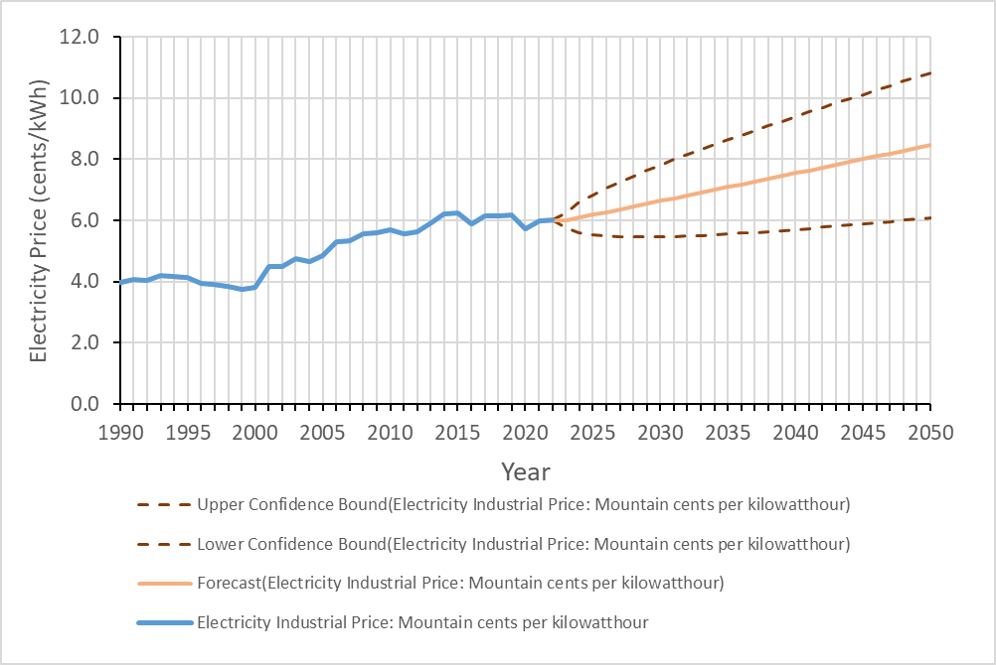
\includegraphics[width=.8\textwidth]{templates/images/Figure-EIA_Electricity_Forecast.png}
\caption[Electricity price forecast]{Price of electricity from the EIA Short-Term Energy Outlook \protect\citep{eia_short-term_2021}, forecast out to 2050.}
\label{fig:electricity_pricing}
\end{figure}

\section{Probabilistic Cost Model}\label{ch4:cm_uncertainties}
The model described thus far takes a deterministic approach; parameter values are fixed to their most-likely values when performing the NPV calculation. A probabilistic approach replaces these static values with distributions and repeatedly samples from those distributions to capture an ensemble of results. This Monte Carlo-style simulation can provide a more realistic assessment of system performance.

However, all variables in the model have some underlying uncertainty, and defining distributions for every variable would add significant complexity to the model with diminishing returns. Variable selection can be performed using sensitivity testing to target the most impactful variables for uncertainty characterization. This helps balance model complexity with representativeness of the physical system. 

Recognizing the full probable range of variable values and the scenarios that trigger them requires a deep understanding of the scientific, engineering, and socio-technical elements influencing a system. For geothermal, subsurface characterization uncertainties play an important role, but so do uncertainties tied to public policy and market dynamics. The limited focus on the issues listed below should be considered fit-for-purpose for this thesis. Further analysis and discussion with subject matter experts on the local, state, and national levels is advised for similar analysis applied to an active geothermal project.

\subsection{Model Uncertainties}\label{ch4:model_uncertainties}
\subsubsection{Carbon Taxation}\label{ch4:carbon_tax_uncertainty}
\begin{wrapfigure}{R}{0.5\linewidth}
\centering
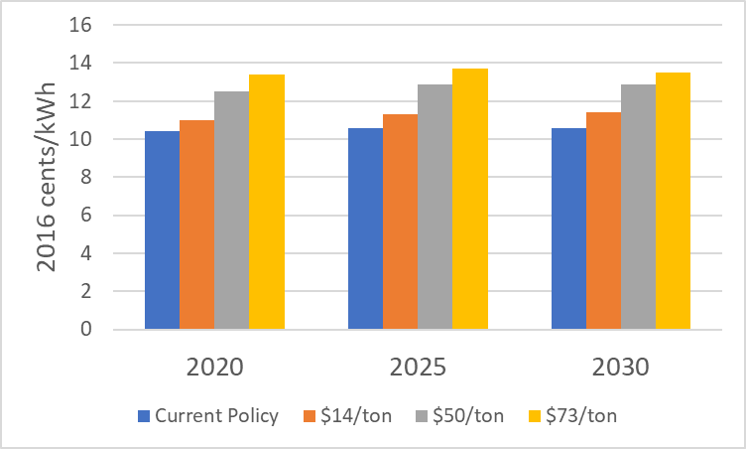
\includegraphics[scale=0.6]{templates/images/Figure-Carbon_Tax_Price_Impact.png}
\singlespacing
\caption[Carbon tax price impact]{National average retail electricity price changes with benchmark levels of carbon taxation, after \protect\citep[Figure\ 30]{larson_energy_2018}.}
\label{fig:carbon_tax_pricing}
\end{wrapfigure}
One proposal for advancing the energy transition to more renewable and sustainable energy solutions involves a carbon tax levied on fossil fuels. The SIPA Center on Global Energy Policy at Columbia University recently studied three analytical scenarios based on federal agency benchmark taxation rates of \$14/ton, \$50/ton, and \$73/ton CO$_2$ equivalent with annual percentage rate increases of 3, 2, and 1.5\%, respectively \citep{larson_energy_2018} (Figure \ref{fig:carbon_tax_pricing}). Their analysis forecasts the impact on electricity pricing out to 2030, with relatively steady-state implications that depend on the specified carbon tax rate. In all taxation cases, electricity prices increase over the present-day, no-tax scenario, likewise boosting the value of a zero-emissions geothermal power relative to fossil fuel-based options. The selected value range for sensitivity testing was a 0-28\% increase in wholesale price, which matches Figure \ref{fig:carbon_tax_pricing}.

\subsubsection{Future Electrification}\label{ch4:electrification_uncertainty}
NREL published a report earlier this year outlining the potential impact of heightened public trends away from non-electric sources of consumed energy, otherwise known as widespread electrification \citep{murphy_electrification_2021}. Some key findings include: (i) end-use natural gas consumption decreases, but so do natural gas prices, which can lead to an increase in natural gas-fueled power plants -- assuming no curtailments due to fossil fuel policies, (ii) deployment of renewables will intensify overall, and (iii) local resources, potentially including new renewable electricity generation facilities, will be relied on to mitigate the need for long-distance electricity transmission \citep{murphy_electrification_2021}.

\begin{wrapfigure}{R}{0.6\linewidth}
\centering
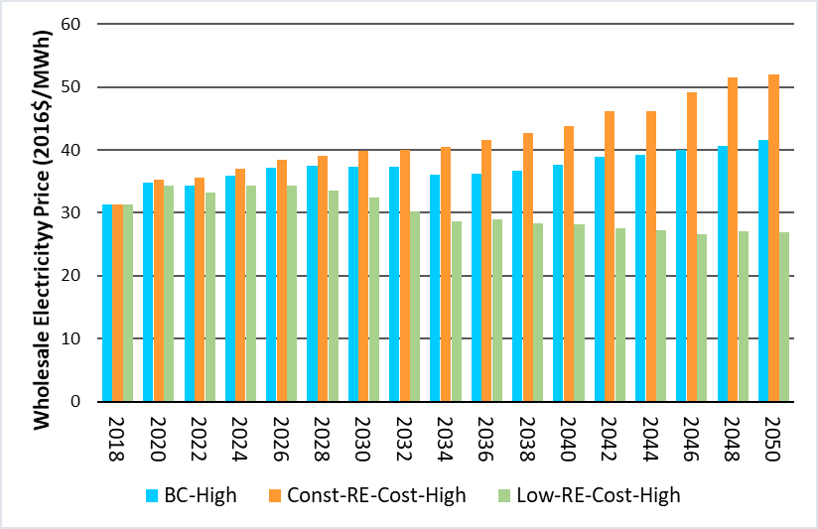
\includegraphics[scale=0.65]{templates/images/Figure-EFS_SIPA_Results.png}
\singlespacing
\caption[Electrification price impact]{Wholesale electricity price forecasts for high future electrification scenarios: base case (blue), constant renewable technology cost (orange), and low renewable technology cost (green). Cases are from the NREL Electrification Futures Study \protect\citep{murphy_electrification_2021}. Figure is adapted from interactive plots at \url{https://cambium.nrel.gov/? project=fc00a185-f280-47d5-a610-2f892c296e51.}}
\label{fig:EFS_electricification}
\end{wrapfigure}
The issue of national electrification is quite complex, particularly for the interplay between the natural gas market and renewables. Additional dependencies include infrastructure upgrades and development to handle growing capacity, as well as local effects (e.g., permitting, water or electrical transmission, community support) that act as enablers or hurdles to building a new renewable-fueled power plant or expanding on existing power facilities. One way to simplify a model representation of widespread electrification is to incorporate swings in electricity prices similar to the scenarios shown in Figure \ref{fig:EFS_electricification} with the caveat that other related factors (e.g., federal and state-level incentive programs or infrastructure improvements) can also influence the bottom line for a geothermal project. Based on NREL projections for High Future Electrification cases, wholesale electricity prices in 2050 could vary from 23\% lower than the 2020 base case rate for the Low Renewable Technology Costs case, to 50\% greater for the Constant Renewable Technology Costs case (Figure \ref{fig:EFS_electricification}). Therefore, -23\% and +50\% define the range of price factors used for sensitivity testing.
\\
\\
\subsubsection{Climate Change}\label{ch4:climate_uncertainty}
\begin{wraptable}{R}{0.58\linewidth}
\centering
\begin{tabular}{|l|c|c|}
\hline
\multicolumn{1}{|c|}{\textbf{Region}} & \textbf{RCP4.5} & \textbf{RCP8.5} \\ \hline
Northeast & 3.98 & 5.09 \\ \hline
Southeast & 3.40 & 4.30 \\ \hline
Midwest & 4.21 & 5.29 \\ \hline
Great Plains North & 4.05 & 5.10 \\ \hline
Great Plains South & 3.62 & 4.61 \\ \hline
\textbf{Southwest} & 3.72 & 4.80 \\ \hline
Northwest & 3.66 & 4.67 \\ \hline
\end{tabular}
\caption[Projected regional temperature changes]{Projected average temperatures in $^\circ$F for mid-century (2036-2065) relative to the 1976-2005 average baseline under lower emissions (RCP4.5) and higher emissions (RCP8.5) scenarios, adapted from \protect\citep[Table 6.4]{vose_temperature_2017}. New Mexico is included in he Southwest region, highlighted in bold.}
\label{tab:reg_climate}
\end{wraptable}

The $1.5^\circ$C climate change goal described in the 2018 IPCC special report \citep{ipcc_global_2018} refers to a global average, so more extreme temperature changes are expected to occur on a local scale even if this target gets met. New Mexico, a state already known for semi-arid conditions, is at risk of encountering warming far in excess of $1.5^\circ$C by 2050 (Table \ref{tab:reg_climate}). The North Carolina Institute for Climate Studies (NCICS) reports annual average temperatures in NM have already increased $1.1^\circ$C since the 1970s, and the observed number of days with maximum temperatures of $100^\circ$F ($37.8^\circ$C) or higher is rapidly climbing \citep{frankson_new_2019}.

Geothermal plant performance is sensitive to the temperature difference between the hot and cooled states of the working fluid. For air-cooled binary plants, changes in ambient temperature could impact overall power plant generation potential. In fact, geothermal power output typically shows seasonality, sometimes with variances of several percentage points in thermodynamic efficiency between winter and summer \citep[p.\ 52]{glassley_geothermal_2015}.  

\citeauthor{frankson_new_2019} present a range of model scenarios for temperature changes in New Mexico related to climate change (\citeyear[Figure 1]{frankson_new_2019}). The high emissions case predicts an average of $\approx 2.7^\circ$C and a maximum of $\approx 4.2^\circ$C increase in state-wide temperatures by 2050. An adjustment of 0-4.2$^\circ$C is therefore applied to this variable for cost model sensitivity testing.

\subsubsection{Drilling \& Completions}\label{ch4:drilling_uncertainty}
Studies on Enhanced Geothermal Systems (EGS) consistently show drilling-related costs are the primary contributor to overall expenses --- up to 60-75\% of the total cost of an EGS project \citep{lukawski_uncertainty_2016}. According to annual benchmark standards published by \citet{nrel_2020_2020}, future advances in geothermal drilling technology will need to include more efficient penetration rate and bit life, new casing methods that reduce drilling time, and reductions in drilling material consumption as wells are completed faster. All aspects of stimulation also need to show improved economics to drive down costs \citep{nrel_2020_2020}.

\begin{figure}[!htp]
\centering
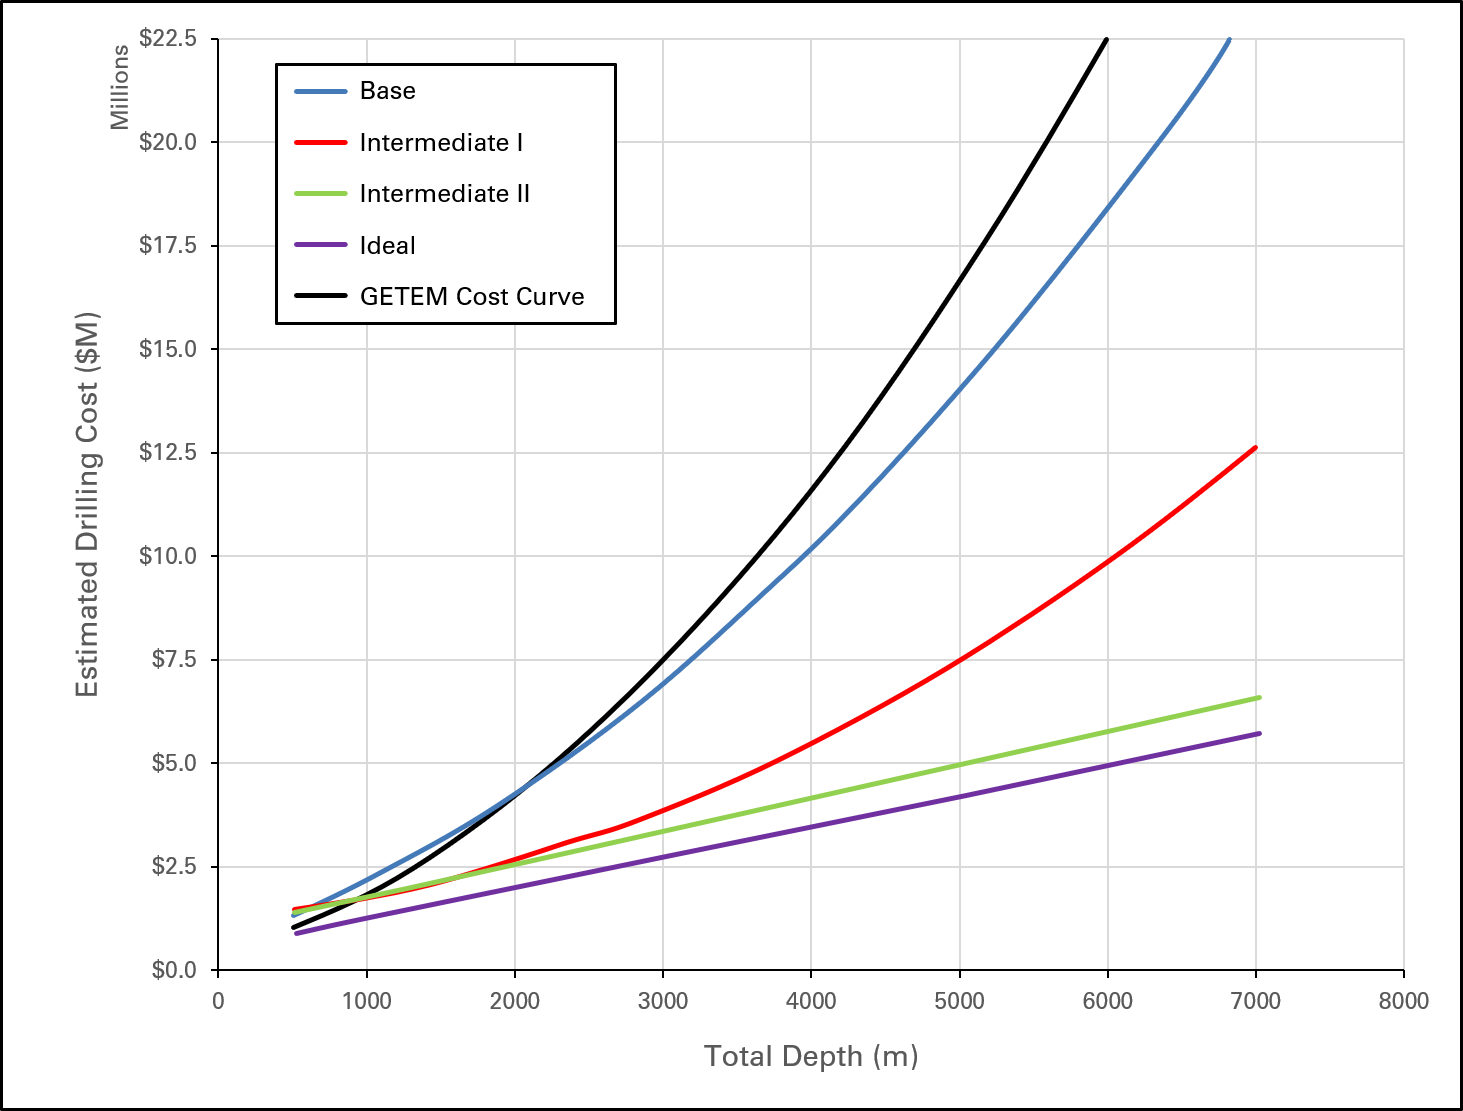
\includegraphics[width=0.8\textwidth]{templates/images/Figure-Drilling_Cost_Curves.png}
\singlespacing
\caption[GeoVision drilling cost curves]{Drilling cost curves in \$M USD per meters depth for a large-diameter open-hole vertical well, adapted from \citep[Figure 8]{augustine_geovision_2019}}
\label{fig:drill_cost_curves}
\end{figure}

Multiple scenario-based drilling cost curves were derived as potential updates for the GETEM model in association with the 2017 GeoVision study (Figure \ref{fig:drill_cost_curves}) \citep{lowry_implications_2017}. A number of key assumptions about changes in geothermal drilling technology went into the creation of these curves \citep{augustine_geovision_2019}:

\begin{itemize}[itemsep=2pt]
    \item Bit life and rate of penetration scale from 2-4$\times$ faster than the base case.
    \item Number of casing intervals incrementally reduces to just one for the ideal case.
    \item Mud costs decline as greater fractions of the well use air drilling techniques.
    \item Logging while drilling (LWD) replaces wireline drilling for up to the entire well length in the ideal case.
    \item Contingency costs related to unexpected or adverse conditions drop from 15\% to 0\% across the four cases.
    
\end{itemize}
Based on the cost curves in Figure \ref{fig:drill_cost_curves} and the anticipated depths for the target reservoir in the Lighting Dock expansion, the selected range of drilling costs to test for model sensitivity is \$1-\$3 million.

\subsubsection{Thermal Drawdown Rate}\label{ch4:drawdown_uncertainty}
Much like wells used for water or oil \& gas operations, geothermal wells generate a drawdown effect from production activities. The thermal drawdown rate defines how quickly the heat content (enthalpy) accessible within the reservoir fracture network declines over time. As thermal drawdown increases, the temperature of produced fluids decreases, as does the amount of electricity generated by the binary cycle process.

Recent EGS studies suggest 0.5-0.6\%/year is an appropriate drawdown rate for EGS applications \citep{augustine_geovision_2019}, although more pessimistic assessments range from 1.5\%/year \citep{beckers_low-temperature_2016}, to 3.3\%/year \citep{augustine_comparison_2006} and 4\%/year \citep{tester_economic_1990}. End-cap values of 0.5\% and 4\% are used for sensitivity analysis.

\subsubsection{Geothermal Gradient}\label{ch4:gradient_uncertainty}
As a blind geothermal system with no original surface expression, the Lightning Dock discovery came after anomalously high temperature gradients (and boiling water) were found in local agricultural wells \citep{crowell_history_2014}. Table \ref{tab:ld_gradient_holes} lists bottom hole temperatures for wells drilled within a 0.5-4.0 km distance from the field-central TFD55-7 well during the 2001-2004 Geothermal Resource Evaluation and Definition (GRED) program \citep{cunniff_final_2005}. Note that the Gradient column describes a linear fit from an assumed surface temperature of 15$^\circ$C to BHT, potentially over-simplifying complex temperature relationships with depth. The gradients in the Reported column come from more reliable assessments near well total depth as documented by \citet{cunniff_final_2003}. 
\\
\begin{table}[!htp]
\centering
\begin{tabular}{|l|c|c|c|c|}
\hline
\textbf{Well Name} & \textbf{Depth (m)} & \textbf{BHT ($^\circ$C)} &
\textbf{\begin{tabular}[c]{@{}c@{}}Gradient\\(K/km)\end{tabular}} &
\textbf{\begin{tabular}[c]{@{}c@{}}Reported\\(K/km)\end{tabular}} \\ \hline
\textbf{TG12-7} & 305 & 69 & 177 & 120 \\ \hline
\textbf{TG56-14} & 381 & 36 & 55 & 80 \\ \hline
\textbf{TG36-7} & 305 & 90 & 246 & - \\ \hline
\textbf{TG57-7} & 278 & 108 & 335 & - \\ \hline
\textbf{TG52-7} & 771 & 137 & 158 & - \\ \hline
\end{tabular}
\caption[Lightning Dock well data]{Examples of Lightning Dock geothermal gradients from bottom hole temperatures (BHT). Gradient is a linear approximation assuming 15$^\circ$C at the surface. The two Reported gradients use temperature log trends near TD. Table adapted from \protect\citep[Table\ 1]{cunniff_final_2005}.}
\label{tab:ld_gradient_holes}
\end{table}

Thermal models calibrated to these wells show local gradients in excess of 300 K/km near the field center and temperature inversions on the flanks of the main Lightning Dock thermal anomaly \citep[see Figs.\ 23-24]{cunniff_final_2005}. Away from this fault-centered hydrothermal plume --- where an EGS expansion project would be targeted --- the thermal field settles into a more traditional monotonically-increasing depth trend. Wells TG12-7 and TG56-14, located 1 km and 4 km away from TFD55-7, respectively, have reported gradients of 80-120 K/km. This range is used for testing model sensitivity to thermal gradient variations.

\subsection{Sensitivity Testing}\label{ch4:sensitivity}
Selecting which of the uncertainties discussed in Section \ref{ch4:cm_uncertainties} should be treated as probabilistic values in the cost model requires testing the sensitivity of NPV to model adjustments bounded by the uncertainty ranges. Specifically, NPV is recalculated after changing a single model variable at a time to match the extremal values outlined in the previous discussion. The full NPV calculation follows the model descriptions given in Sections \ref{ch4:cm_npv}-\ref{ch4:cm_params}, with the exception of price-related uncertainties, which are modeled by changing the price annually to mimic the most price-sensitive scenario where PPAs are market-based rather than fixed. No flexibility is assumed for this exercise, so the full power plant expansion takes place at the start of the 30-year timeline. Also, this analysis uses the version of the static model where production flow rate is prescribed at 40 kg/s (see Table \ref{tab:cm_resource_params}) and the capacity per module depends only on the temperature of the produced brine. The reasons for this choice of model structure over one where power output is strictly capped at 5 MW are discussed further in Chapter \ref{ch6:cm_results}.

The tornado diagram in Figure \ref{fig:tornado} provides a simple visualization of model sensitivity based on NPV calculation results for the different uncertainties, sorted in order of descending importance. Results also appear in Table \ref{tab:tornado_table}. The baseline static model predicts a NPV of $\approx \$91,000$. Results deviate from baseline most significantly for thermal drawdown rate; when no measurable drawdown takes place, NPV reaches \$18 million, but predicted losses top \$47 million if the drawdown rate is as high as 4\%. Uncertainties related to drilling costs, future electrification, and the geothermal gradient all show moderate importance for project NPV. Changes to ambient surface temperature (i.e., due to climate change) and pricing from carbon taxation both have an order of magnitude less influence on project NPV than other uncertainties. Based on this sensitivity test, variables tied to the top 4 uncertainties will be treated as random variables for a probabilistic NPV model.

\begin{figure}[!htp]
\centering
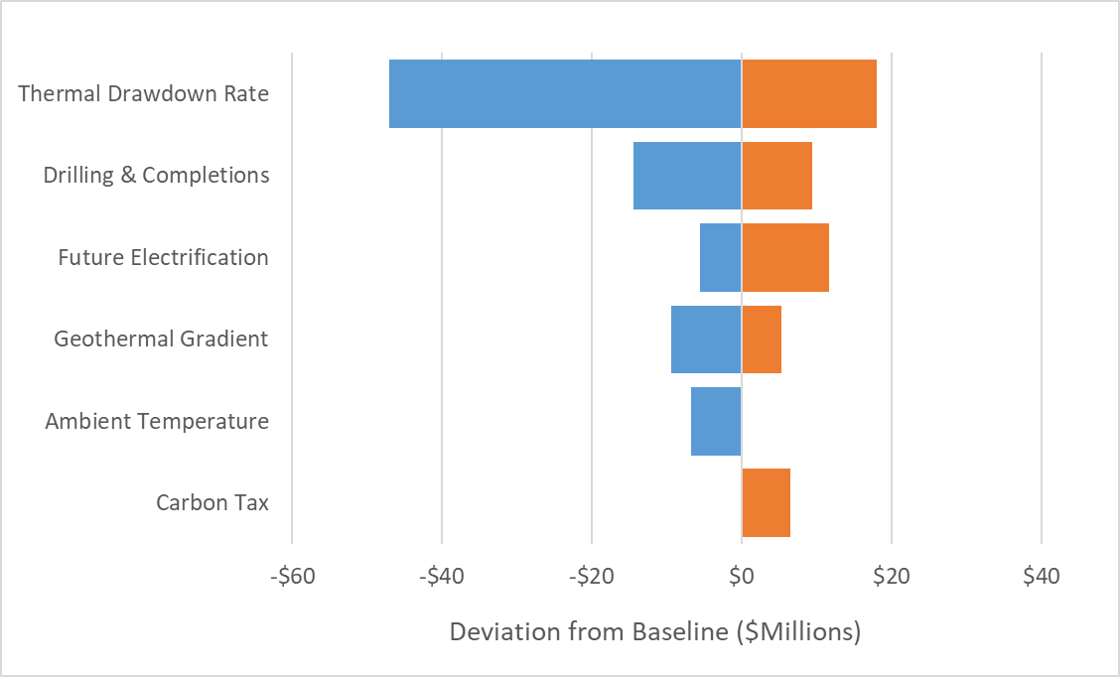
\includegraphics[width=0.8\textwidth]{templates/images/Figure-Tornado.png}
\singlespacing
\caption[Sensitivity testing tornado diagram]{Tornado diagram showing NPV model sensitivity to different system uncertainties for the proposed Lightning Dock expansion. X-axis measures deviation from base case when all plant construction takes place at project start and the model parameterization matches Tables \ref{tab:cm_resource_params}-\ref{tab:cm_econ_params}. Values are in \$M USD, where M indicates millions.}
\label{fig:tornado}
\end{figure}

\begin{table}[!htp]
\centering
\begin{tabular}{|l|c|c|c|}
\hline
\textbf{} & \textbf{Low (\$M)} & \textbf{High (\$M)} & \textbf{Range (\$M)} \\ \hline
\textbf{Thermal Drawdown Rate} & -\$47.0 & \$18.0 & \$65.0 \\ \hline
\textbf{Drilling \& Completions} & -\$14.5 & \$9.4 & \$23.9 \\ \hline
\textbf{Future Electrification} & -\$5.5 & \$11.7 & \$17.2 \\ \hline
\textbf{Geothermal Gradient} & -\$9.4 & \$5.4 & \$14.7 \\ \hline
\textbf{Ambient Temperature} & -\$6.7 & -\$0.1 & \$6.6 \\ \hline
\textbf{Carbon Tax} & -\$0.1 & \$6.5 & \$6.6 \\ \hline
\end{tabular}
\caption[Sensitivity testing results]{Results of NPV model sensitivity testing for different system uncertainties associated with the Lightning Dock expansion. NPV values are listed in \$M USD, where M indicates millions.}
\label{tab:tornado_table}
\end{table}

\subsection{Probability Density Functions}\label{ch4:pdfs}
Having established which uncertainties impact the cost model the most, \acrlong{pdf}s (\acrshort{pdf}s) can be assigned to model variables for use as part of a stochastic NPV assessment. Running the model multiple times over generates a Monte Carlo ensemble of NPV solutions, each representing the model response to a different sampling of these variable values. The ensemble can be evaluated using a combination of metrics for individual model analysis or comparison with alternative models. Chapter \ref{ch6:cm_results} outlines the results of the Monte Carlo approach applied to the Lightning Dock expansion cost model using the variable PDFs in figure \ref{fig:cm_probdists} and described below.

\begin{figure}[htp]
\centering
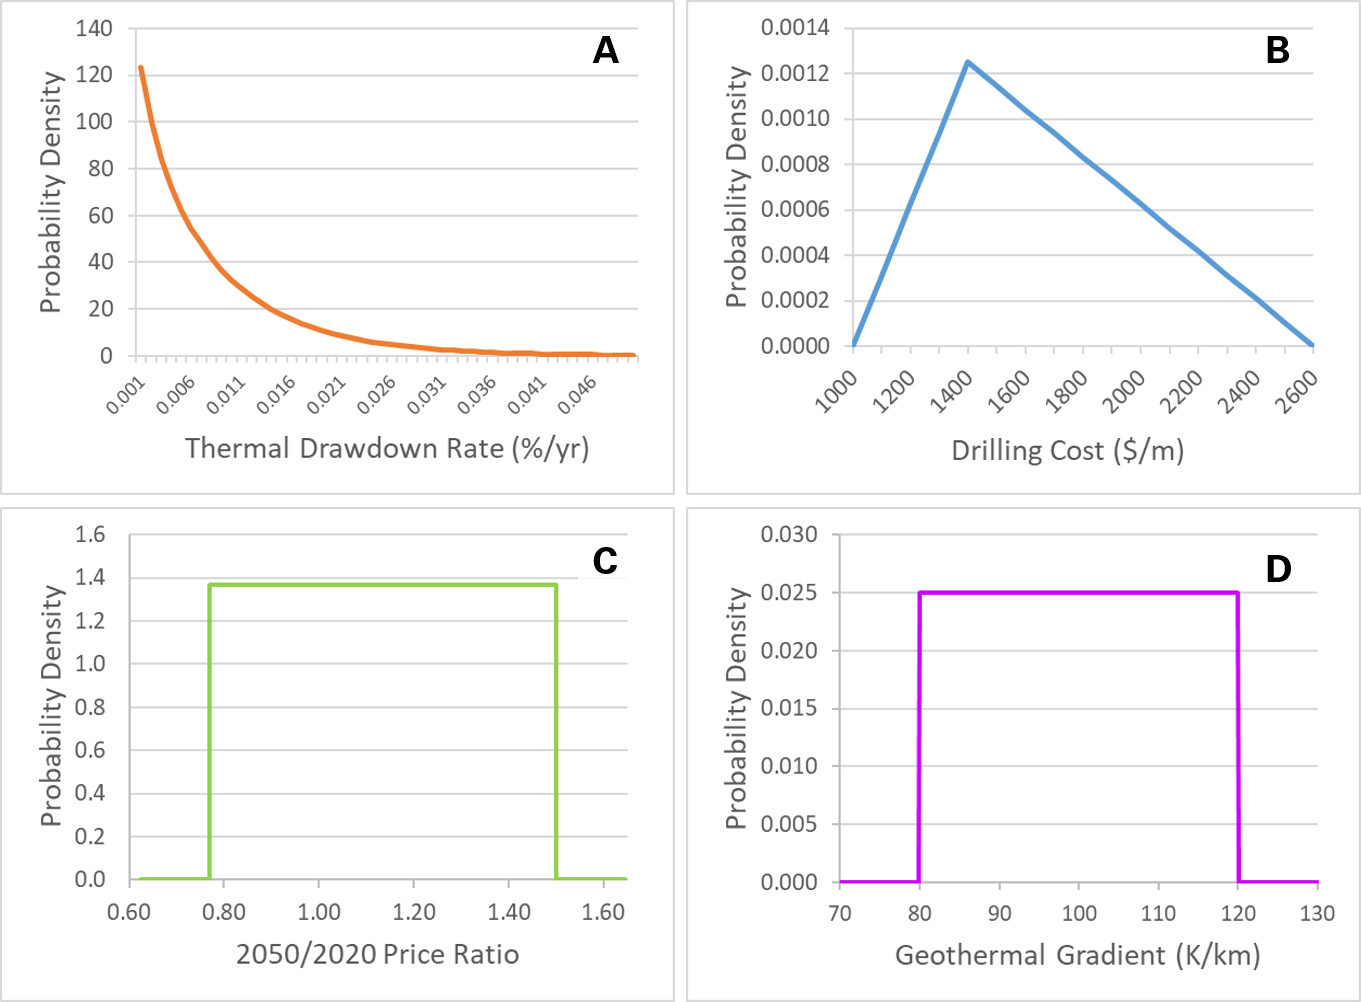
\includegraphics[width=.85\textwidth]{templates/images/Figure-ProbDists.png}
\singlespacing
\caption[Cost model probability distributions]{Probability distribution functions for A. thermal drawdown rate, B. drilling \& completions costs, C. electricity pricing, and D. geothermal gradient.}
\label{fig:cm_probdists}
\end{figure}

\subsubsection{Thermal Drawdown Rate}\label{cm4:prob_tdr}
The latest version of GETEM \citep{mines_getem_2016} and its variant in the NREL System Advisor Model \citep{blair_system_2018} apply 0.5\% as a default value for thermal drawdown rate. Higher decline rates tend to be associated with older models; 1-2\% for GEOPHIRES \citep{beckers_low-temperature_2016}, 3\% in a thesis by \citet{augustine_hydrothermal_2009}, and 4\% for work done in the 1990s by \citet{tester_economic_1990}. The probability density function for thermal drawdown was designed using a beta function such that the P$_{50}$ value aligns with 0.5\% annual drawdown rate, and 4.0\% represents the P$_{97.5}$ case (Figure \ref{fig:cm_probdists}A). Note that the beta function was slightly altered to follow a linear trend from P$_{95}$ to P$_{100}$ to ensure rare extremely high rates in the distribution function do not asymptotically approach over 10\% per year. The highest rate supported by the distribution is 5.6\%.

\subsubsection{Drilling \& Completions Costs}\label{cm4:prob_dc}
Drilling costs for geothermal wells remain a topic of debate due in part to the small number of direct analogs, particularly for EGS wells, and the documented differences with oil \& gas drilling operations. This discrepancy was noted in the 2006 MIT study on EGS, which promoted the use of a dedicated geothermal drilling cost index as a solution \citep{tester_future_2006}. Nevertheless, numerous and sometimes quite disparate relationships have appeared in the years since; for the 1.0-1.5 km drilling depths considered in this study, recent estimates range from a low $\approx\$500$/m \citep{lukawski_uncertainty_2016} to a very high \$2,800/m \citep{lowry_implications_2017}. In order to capture a reasonable spread while recognizing the uncertainty in even defining a distribution shape, geothermal drilling costs are modeled as a triangular distribution (Figure \ref{fig:cm_probdists}B). The midpoint value of \$1400/m comes from the predicted well depth and cost in the static model (see Section \ref{ch4:cm_capex_dc}). The extreme values of \$1000/km and \$2800/km approximate the range shown for depths of 1.0-1.5 km among the drilling cost curves from the recent GeoVision study (Figure \ref{fig:drill_cost_curves}).

\subsubsection{Electricity Pricing}\label{cm4:prob_price}
Electricity prices in the static cost model are determined by the EIA STEO price forecast for the Mountain region (Figure \ref{fig:electricity_pricing}) \citep{eia_short-term_2021}. Two variable price components are superimposed on this trend for the probabilistic model. First, a disruption to the cost curve is simulated by randomly-selecting a year between 2020-2050 and introducing a step-change in price to capture the sudden nature of energy transition events. The magnitude of the step change is determined from a uniform distribution bounded by the range of 2050 High Future Electrification prices relative to the 2020 HFE base case in the Electrification Futures Study (Figure \ref{fig:cm_probdists}C) \citep{murphy_electrification_2021}. An example of how this randomly-timed, randomly-sampled step change affects the price curve is shown in Figure \ref{fig:elec_price_prob}A. 

Second, volatility could also influence the spot price used for setting a power purchase agreement for a given model year. Using the 95\% confidence bounds on the price curve to derive standard deviation, each point in the forecast is replaced by a normal distribution and randomly sampled to produce different price model realizations (Figure \ref{fig:elec_price_prob}B). This curve will regenerate as a unique price projection for each Monte Carlo realization of the cost model.

\begin{figure}[htp]
\centering
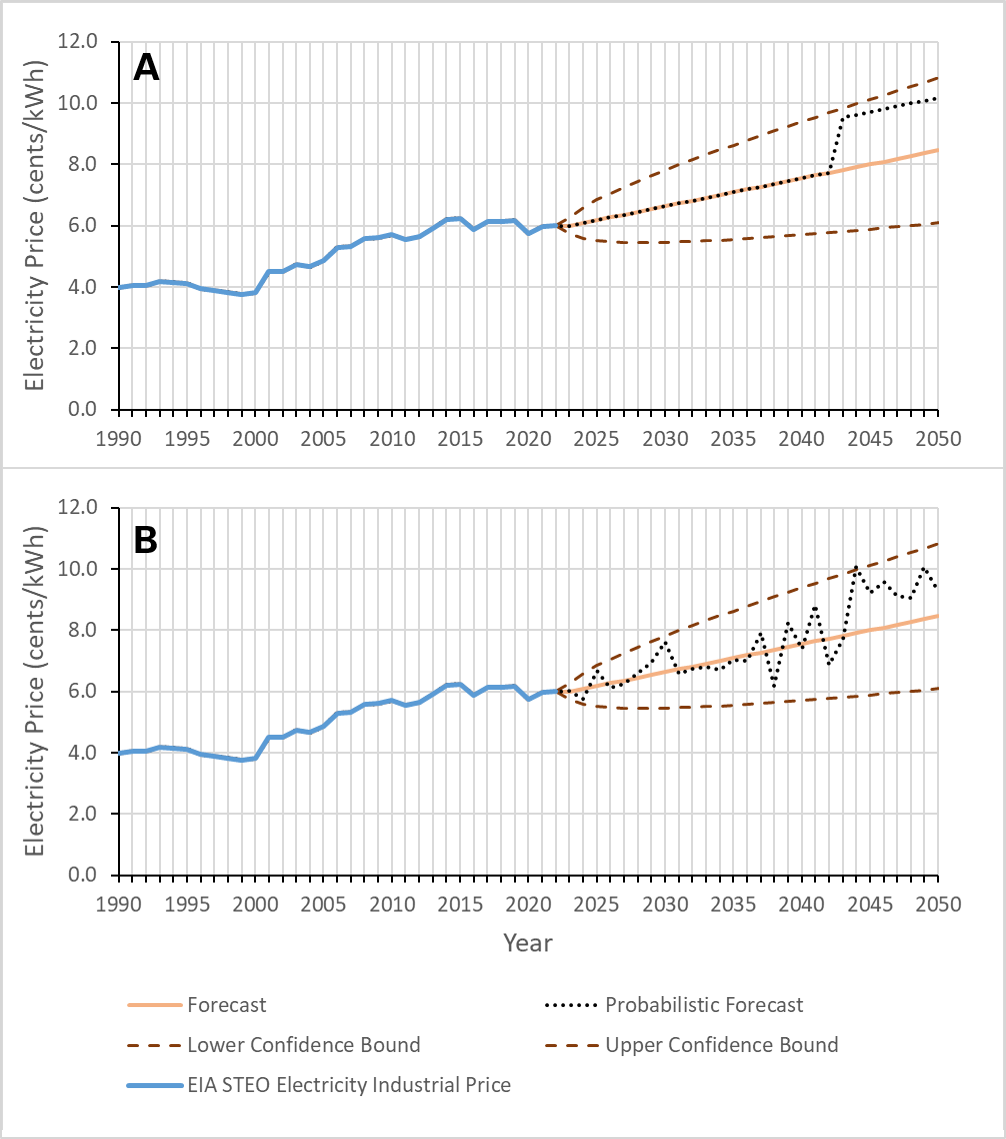
\includegraphics[width=.85\textwidth]{templates/images/Figure-ElectPrice_Prob.png}
\singlespacing
\caption[Cost model probabilistic price forecasts]{EIA STEO electricity industrial prices for the Mountain region (blue), forecast to 2050 (orange) as in Figure \ref{fig:electricity_pricing}, with A. a randomly-defined step change in pricing and B. added annual volatility using the forecast 95\% confidence intervals.}
\label{fig:elec_price_prob}
\end{figure}

\subsubsection{Geothermal Gradient}\label{cm4:prob_gradient}
Local spatial variations in geothermal gradient are difficult to characterize with only a sparse sampling of the Lightning Dock area by predominantly shallow boreholes. Subsurface models like those shown in Figures 22-24 of \citep{cunniff_final_2005} generally predict a smoothly-varying thermal field in areas without direct observational data. But the complex temperature structure associated with the Lightning Dock hydrothermal plume suggests thermal heterogeneity can exist away from the Animas Valley fault. Uncertainty in geothermal gradient is therefore represented in the cost model by a uniform probability distribution with end points determined by measured gradients from wells TG12-7 and TG56-14 (Figure \ref{fig:cm_probdists}D).

\subsubsection{Reservoir Temperature}\label{cm4:prob_temp}
\begin{wrapfigure}{R}{0.55\linewidth} %[htp]
\centering
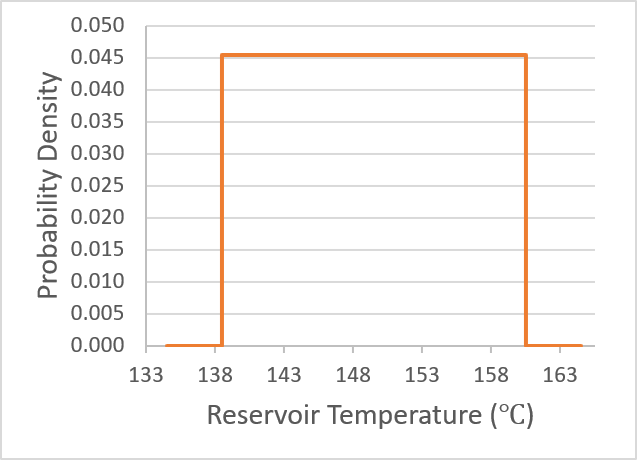
\includegraphics[scale=0.45]{templates/images/Figure-Reservoir_Temp_PDF.png}
\singlespacing
\caption[Reservoir temperature PDF]{Reservoir temperature probability density function. The value range is based on values originally proposed by \protect\citet{schochet_development_2001}.}
\label{fig:cm_temp_pdf}
\end{wrapfigure}
Although not included in the sensitivity testing exercise in Section \ref{ch4:sensitivity}, the original proposal for EGS production at Lightning Dock by \citet{schochet_development_2001} noted a range of likely reservoir temperatures in the Horquilla limestone formation. Geothermal power production relies first and foremost on the subsurface temperatures being ``mined'' by circulating fluids. Uncertainty in initial reservoir temperature is therefore included in the cost model, represented by a uniform probability distribution with bounds determined from the temperatures proposed by \citet{schochet_development_2001} (Figure \ref{fig:cm_temp_pdf}).

\section{Flexibility with Design Options}\label{ch4:flex_design_options}
The addition of probability density functions to the cost model for Monte Carlo simulation provides a means of testing the model response to uncertainties in the system. But this probabilistic Base Case model still remains inflexible in the face of emergent conditions that would trigger actions in a real-life scenario. These actions are sometimes characterized as design options that, like financial options, can be exercised in the future if doing so might benefit system stakeholders \citep[p.\ 270-272]{de_neufville_flexibility_2011}.

Design options can be implemented as decision rules defining how a model behaves based on past observations. Decision rules may act independently or be chained together to mimic complex system flexibilities that can reveal otherwise hidden financial value. The following scenarios extend the Base Case model with one or more decision rules. Chapter \ref{ch6:cm_results} examines how implementing these rules impacts predicted model ENPV, target curves, and other forecast performance measures.

\subsection{Redevelop Only Case}\label{ch4:flex_redevelop_case}
Sensitivity testing revealed thermal drawdown rate as the most important uncertainty governing the cost model performance (Figure \ref{fig:tornado}). Over time, cooling of the reservoir by injected fluids results in declining input temperatures to the binary cycle plant and hence lower electricity production. If the latter drops below a certain level, redrilling or restimulation of the reservoir are required to ensure generation rates remain within a reasonable (or profitable) range. The GETEM model tracks thermal decline and discounts power plant performance until the accessible reservoir temperature reaches a certain threshold defined by \citep{entingh_volume_2006}:
\begin{equation}
\label{eq:drawdown_threshold}
    \Delta T_{max} = (T_f-T_i)_{max} = 0.21 \cdot T_i - 12.2
\end{equation}

Combining this equation with a harmonic decline curve assumption results in the following relationship for the time before the maximum acceptable decline is reached:

\begin{equation}
\label{eq:redevelop_time}
\begin{aligned}
    t &= \frac{1}{D} \cdot 
    \left( {
    \left( {\frac{T_i}{T_f} }\right) - 1
    }\right)\\
    &= \frac{1}{D} \cdot 
    \left( {
    \left( {\frac{T_i}{1.21 \cdot T_i - 12.2}
    }\right) - 1
    }\right) 
\end{aligned}
\end{equation}

To counteract the negative impact of this decline, a full field re-drill campaign is triggered in cost models like GETEM. This may occur several times over the lifespan of a geothermal power plant depending on the drawdown rate, although GETEM freezes re-drills in the final 5 years to ensure no redevelopment cost is incurred just prior to end of life for the facility \citep{entingh_volume_2006}. This methodology is applied here using the following decision rule:
\\
\\
\textbf{Redevelopment Decision Rule}\label{ch4:dr_redevelop}
\begin{enumerate}
	\item Determine the temperature threshold for viable power production using Equation \ref{eq:drawdown_threshold} and the initial reservoir temperature.
	\item Calculate the number of years until the temperature threshold is reached based on the thermal drawdown rate and Equation \ref{eq:redevelop_time}. This defines the redevelopment interval for the field.
    \item In the annual cash flow analysis, determine if time since installation of any power plant modules is a multiple of the redevelopment interval. If so and the year being evaluated does not fall within the final 5 years of the project lifespan:
	\begin{enumerate}
	    \item Identify how many modules need to be redeveloped. Multiply this by 2 to define the number of wells being sidetracked (or redrilled). This assumes the wells are in pairs for each module.
	    \item Calculate CAPEX for redevelopment by multiplying the drilling costs per well by the number of wells being reworked, then discount by the pre-determined redevelopment factor. Scale this by the learning rate discount based on the number of wells already drilled since field operations began.
	    \item Update the running tally of wells drilled or redrilled to include wells from this redevelopment effort.
	    \item Reset the produced brine temperature to the initial reservoir temperature.
    \end{enumerate}
\end{enumerate}

\subsection{Redevelop \& Grow Case}\label{ch4:flex_grow_case}
Redevelopment of the geothermal field is primarily a mitigation against loss of accessible resource as thermal drawdown impacts the flow paths between wells. Capturing upside potential is equally important. The Redevelop \& Grow case recognizes that up-swings in wholesale electricity prices may signal a comprehensive shift in long-term energy pricing due to influences like societal shifts toward electrification. To take advantage of the opportunity, this case considers a price change threshold as the trigger for installing additional geothermal power plant modules and renegotiating the PPA with the local utility company (\textit{Price trigger for flexibility}, see Table \ref{tab:cm_econ_params}). The scenario assumes a flat percentage increase in capacity (\textit{Expansion amount}, see Table \ref{tab:cm_econ_params}) and universal success in establishing new power agreements at a set mark-up percentage above wholesale (\textit{Contract rate over wholesale}, see Table \ref{tab:cm_econ_params}). The field redevelopment decision rule outlined for the Redevelop Only case remains intact, and another decision rule for design flexibility in modular growth is as follows:
\\
\\
\textbf{Capacity Growth Decision Rule}\label{ch4:dr_grow}
\begin{enumerate}
    \item In the annual cash flow analysis, look up the predicted wholesale electricity price for the current year and determine the deviance between this price and the wholesale price used in the last PPA contract (i.e., when the last capacity change took place). Here, deviance is defined as: \(\frac{(\text{current price} - \text{past price})}{\text{past price}}\).
    \item If the deviance exceeds the pre-set price trigger and the year being evaluated does not fall within the final 5 years of the project lifespan:
    \begin{enumerate}
        \item Multiply the number of operating power plant modules in the field by the pre-set expansion parameter to determine the number of modules to add.
        \item Calculate CAPEX for drilling an injector-producer pair for each added module. Scale this value by the learning rate discount based on the number of wells previously drilled or redrilled in the field.
        \item Update the tallies for the number of modules in the field and the number of wells drilled or redrilled to include the added modules and their wells.
        \item Determine the new PPA contract price by multiplying the predicted wholesale electricity price for the current year by the pre-determined contract rate above wholesale factor.
    \end{enumerate}
\end{enumerate}

\subsection{Full Flexibility Case}\label{ch4:flex_reduce_case}
Price swings can go the opposite direction as well. The NREL Electrification Futures Study \citep{murphy_electrification_2021} identified scenarios where electricity prices fall between 2020 and 2050, so having a means of addressing a future with tighter margins would be a useful flexibility. In the Full Flexibility Case, field redevelopment with thermal degradation and capacity increases in response to price surges remain in effect. In addition, a sudden drop in electricity prices (\textit{Price trigger for flexibility}, see Table \ref{tab:cm_econ_params}) serves as a trigger for the power plant operator to remove or decommission a number of binary cycle modules (\textit{Reduction amount}, see Table \ref{tab:cm_econ_params}). Since modules operate independently with their own injector-producer couplet, they can be individually decommissioned with no impact on other installed modules in the aggregate facility. Additional cost savings might be realized if the modules are leased and equipment can be returned early to the vendor when no longer in use, although for the sake of simplicity, this option has not been included in the cost model. The decision rule for price-based decommissioning of active modules is as follows:
\\
\\
\textbf{Capacity Reduction Decision Rule}\label{ch4:dr_reduce}
\begin{enumerate}
    \item In the annual cash flow analysis, look up the predicted wholesale electricity price for the current year and determine the deviance between this price and the wholesale price used in the last PPA contract (i.e., when the last capacity change took place). Here, deviance is defined as: \(\frac{(\text{current price} - \text{past price})}{\text{past price}}\).
    \item If the deviance is negative and exceeds the pre-set price trigger (in magnitude), and the current year does not fall within the final 5 years of the project lifespan:
    \begin{enumerate}
        \item Multiply the number of operating power plant modules in the field by the pre-set reduction amount parameter to determine the number of modules to decommission.
        \item Reduce the count of operating modules in the field to account for taking these modules offline.
        \item Make sure OPEX is only calculated for operating power plant modules.
        \item Do \underline{not} reduce the running tally of wells drilled or redrilled. Shutting down modules does not negate the learning experience of drilling the wells associated with those modules.
    \end{enumerate}
\end{enumerate}

\section{Recap} \label{ch4:recap}
This chapter covered the methodology for using cost models to mitigate the risk of expanding an existing power facility with geothermal production. The Lightning Dock KGRA and present-day power plant are the subject of a hypothetical 5 MW EGS expansion project. The model assumes a 30-year useful life for the expansion, and construction is based on the deployment of pre-fabricated binary cycle modules with one injector-producer pair per module.
\\
\\
The modeling strategy follows a step-wise increase in model complexity:
\begin{enumerate}
    \item Start with a static model that calculates NPV based on estimates for Revenue, CAPEX, and OPEX. The model includes thermal drawdown of the reservoir, power plant degradation, a learning rate for drilling costs, and a discount rate for the time value of money. All parameters are pre-defined.
    \item Replace the static model with a probabilistic one by assigning probability density functions to key model parameters. Sensitivity testing high-grades which variables to treat as uncertain in the model. Results are obtained through Monte Carlo sampling to build a solution ensemble, evaluated by multiple measures like ENPV, target curves, and NPV percentiles. The key variables defined with probability distributions in this analysis include: thermal drawdown rate, drilling \& completions costs, electricity pricing, geothermal gradient, and reservoir temperature.
    \item Incorporate flexibility with design options as decision rules in the probabilistic model. The decision rules being evaluated in this analysis include: field redevelopment due to thermal drawdown, growth in capacity when prices surge, and capacity reductions when prices decline.
\end{enumerate}

Results from the application of these methods are explored in Chapter \ref{ch6:cm_results}. 
\chapter{Analytics Application}\label{ch5:expl_applied}

\section{Data Modeling}

\begin{wrapfigure}{R}{0.45\linewidth}
\centering
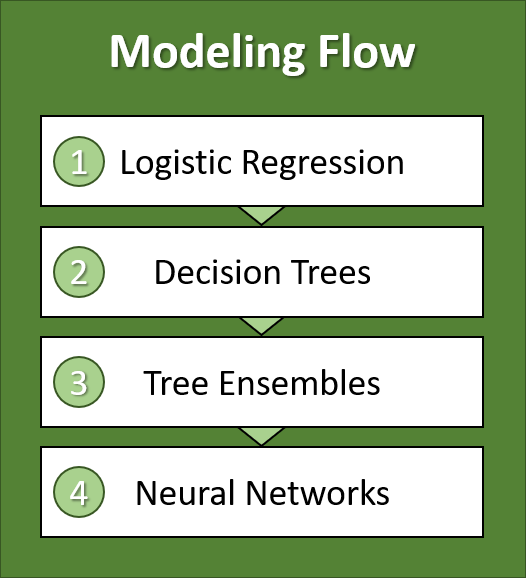
\includegraphics[scale=.6]{templates/images/Flow-Modeling.png}
\singlespacing
\caption[Modeling workflow]{Workflow for predicting the class of geothermal gradient across the southwestern NM study area using a variety of common machine learning methods.}
\label{fig:model_flow}
\end{wrapfigure}

Supervised learning methods for classification come in a wide variety of shapes and sizes. Rather than settle on one for predicting geothermal gradient, four different methods are applied to the southwestern NM data set. Figure \ref{fig:model_flow} illustrates the high-level modeling flow, where model complexity increases with successive steps. The method descriptions below only briefly delve into important model mechanics and key hyperparameters (i.e., parameters not learned from data) that impact model performance. Other sources can provide a deeper review of machine learning algorithms and their mathematical underpinnings. This investigation should instead be considered an applied case study that uses these algorithms as tools for generating insights on geothermal potential. 

\subsection{Assessing Performance}
Building an intuition for the differences in predictive ability of different models first requires a clear definition of the scoring metric(s) used to compare those models. The characterization of classifier performance typically begins with a confusion matrix. In its simplest form, the confusion matrix evaluates class predictions as \acrlong{tp} (\acrshort{tp}; predicted 1, actually 1), \acrlong{tn} (\acrshort{tn}; predicted 0, actually 0), \acrlong{fp} (\acrshort{fp}; predicted 1, actually 0), and \acrlong{fn} (\acrshort{fn}; predicted 0, actually 1). For the multi-class problem, the confusion matrix expands to include all correct classification and mis-classification options. Figure \ref{fig:confusion_matrix} illustrates the elements of a 4-class matrix.

\begin{figure}[!htp]
\centering
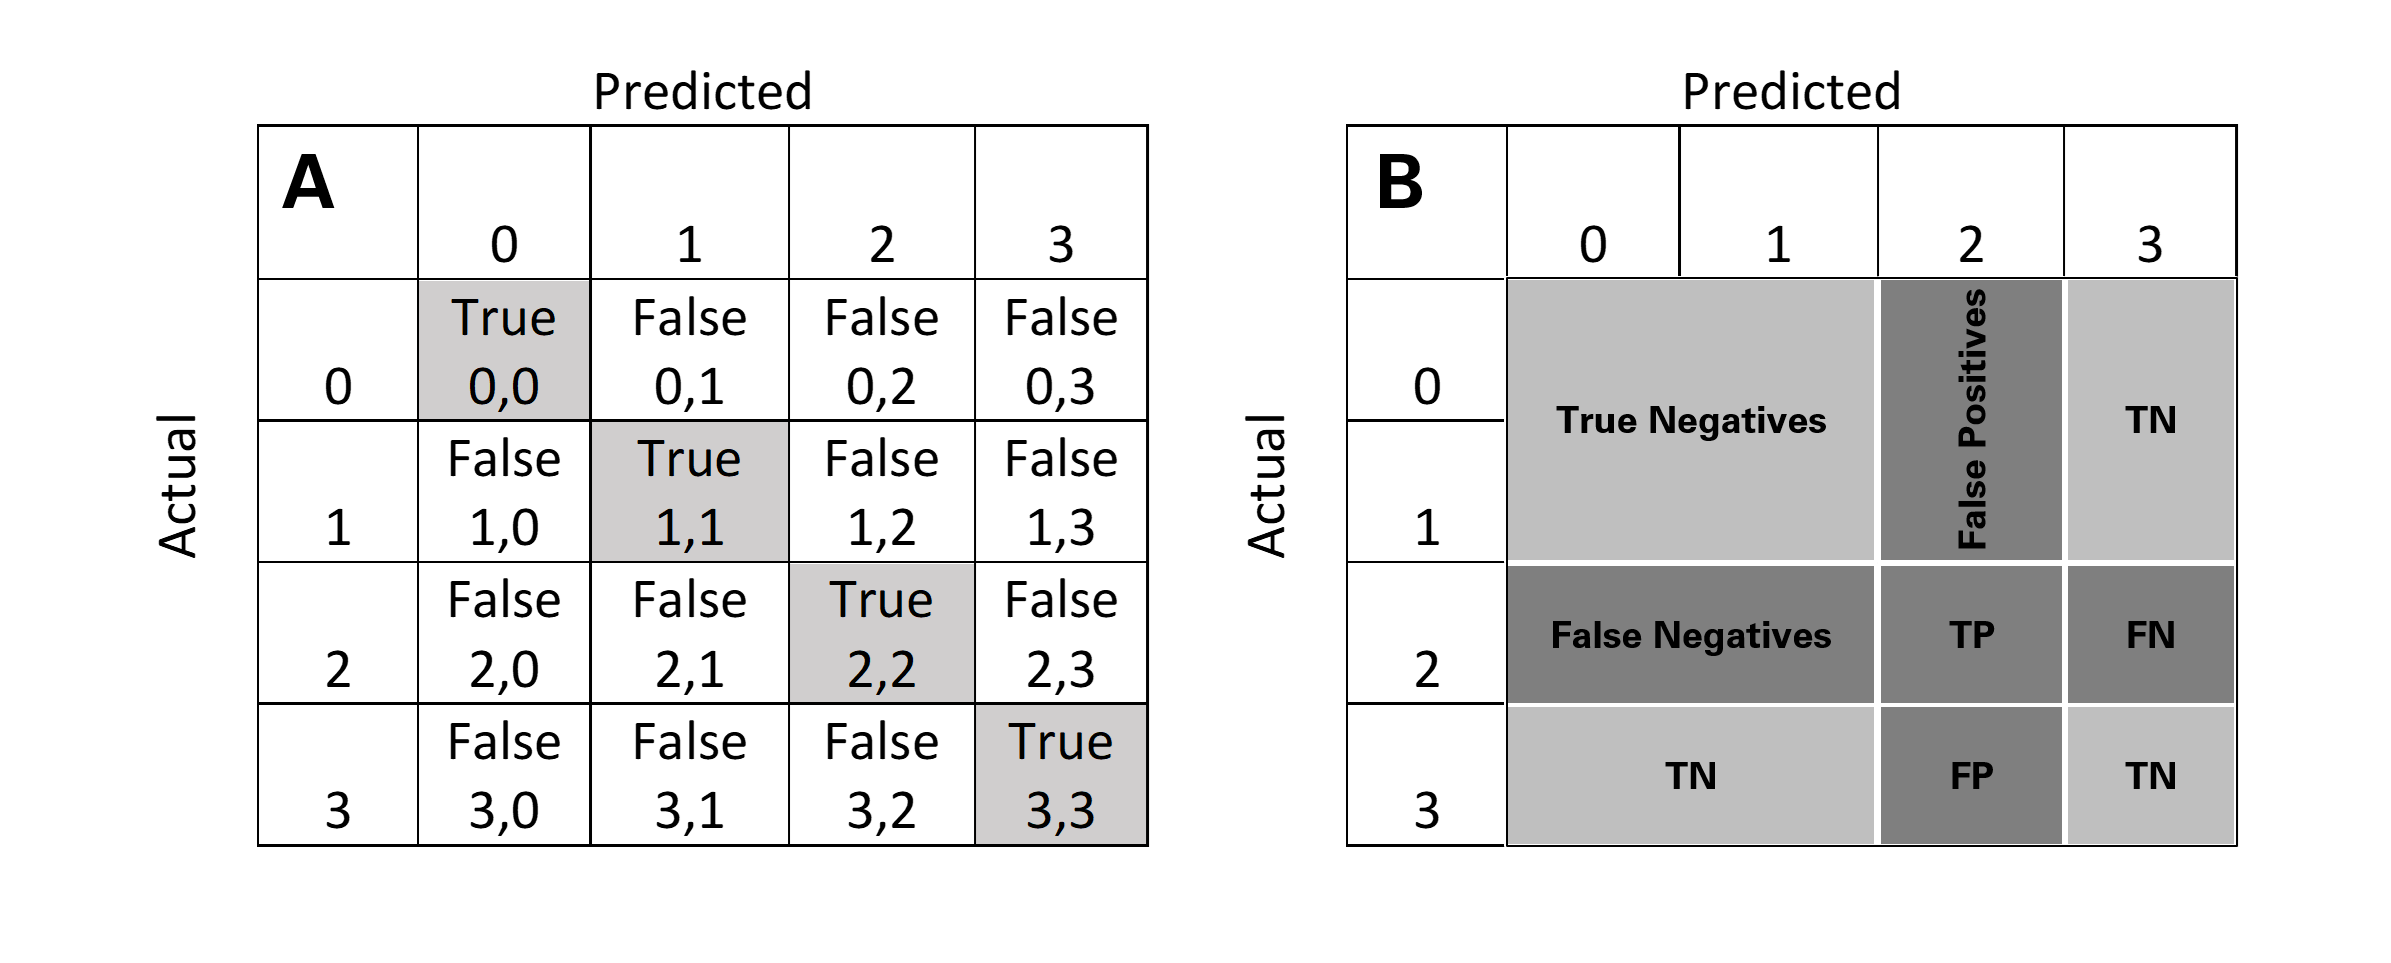
\includegraphics[width=\textwidth]{templates/images/Figure-Confusion_Matrix.png}
\caption[Four-class confusion matrix]{Confusion matrix diagram for a 4-class scenario. A. Each cell represents a pairing between an actual class label (rows) and the predicted label (columns). True positives for each class are down the diagonal. B. Example of matrix interpretation using class 2 as a point of reference. Elements associated with TP, FP, TN, and FN values are labeled.}
\label{fig:confusion_matrix}
\end{figure}

Several statistical measures can be defined using combinations of elements in the confusion matrix. Of significance to this study are the \acrlong{tpr} (\acrshort{tpr}) and \acrlong{fpr} (\acrshort{fpr}) \citep{tharwat_classification_2020}:

\begin{itemize}
\item \textbf{True Positive Rate}: the count of correctly-predicted positives scaled by the actual positives: TP/(TP$+$FN).
\item \textbf{False Positive Rate}: the count of incorrectly-predicted positives scaled by the actual negatives: FP/(FP$+$TN).
\end{itemize}

Classification relies on a probability threshold for assigning a class label. As the threshold lowers, the chances the classifier will believe it has a label match will increase. By varying this threshold, it becomes possible to map out the discriminating ability of a classifier by plotting a curve in TPR vs. FPR space (Figure \ref{fig:roc}). This is commonly referred to as the \acrlong{roc} (\acrshort{roc}) curve \citep{fawcett_introduction_2006}. A classifier that cannot discriminate between classes will perform no better than random guessing, resulting in a curve that plots along the diagonal from the origin to the upper right of the plot. On the other hand, a perfect classifier will have a TPR of 1.0 for all thresholds, so it plots straight up along the y-axis and then horizontally at TPR = 1.0. Typical ROC curves plot in the upper-left space between these two extremes.

\begin{figure}[!htp]
\centering
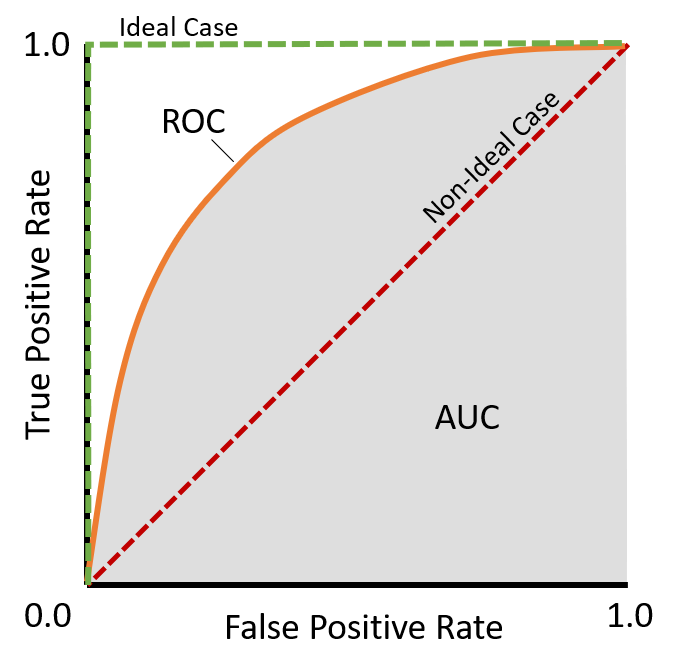
\includegraphics[width=0.5\textwidth]{templates/images/Figure-ROC_AUC_Diagram.png}
\caption[Receiver Operating Characteristic diagram]{ROC curve diagram in TPR vs. FPR space. Perfect classifiers will plot along the ideal case line (green), poor classifiers plot along the diagonal (red). AUC (gray) characterizes the quality of the classifier on a scale of 0.5 to 1.0.}
\label{fig:roc}
\end{figure}

Area Under the ROC Curve (AUC) defines a summary statistic for the ROC function (see Figure \ref{fig:roc}) \citep{fawcett_introduction_2006}. Since the ideal classifier has a TPR of 1.0 at all times, the ideal AUC also equals 1.0. In the non-ideal case, the AUC drops to 0.5. AUC values and ROC curves provide a standardized means of comparing classifiers and are the primary performance metric used in this thesis.

With multi-class classification, defining single class performance using the definitions of TP, FP, TN, and FN as shown in Figure \ref{fig:confusion_matrix}B is relatively straight-forward. Overall classifier performance across all classes can also be characterized with a single ROC curve using macro, weighted, or micro averaging \citep{scikit-learn_sklearnmetricsroc_auc_score_2021}.

\begin{itemize}
    \item \textbf{Macro}: averaging matches the unweighted arithmetic mean of metric values.
    \item \textbf{Weighted}: averaging follows the procedure of macro-averaging but adds a weight for each class contribution based on the fraction of total observations that fall within that class. 
    \item \textbf{Micro}: averaging considers class results in aggregate, so statistics are calculated across the entire confusion matrix. TPR becomes the accuracy and FPR becomes the error rate.
\end{itemize}

For imbalanced data sets, micro will indicate better performance than macro due to the impact of the dominant class. Both micro and macro averages are included in the classification analysis in the following sections.

\subsection{Logistic Regression} \label{ch5:log_reg}

\subsubsection{Binary Formulation} 

The classic \acrlong{lr} (\acrshort{lr}) model is a binary classifier that predicts one of two labels based on the input data. LR frames the problem as a linear combination of the input observations \citep[~p 369]{bertsimas_analytics_2016}:

\begin{equation}
\label{eq:logreg_form}
    y = W^TX = w_0 + w_1 * x_1 + w_2 * x_2 \ldots + w_n * x_n 
\end{equation}

Where $x_i$ are the feature observations, $w_i$ are coefficients or weights for those features, and $y_i$ is a weighted sum. Solving for the weights in this equation ($w_i$) requires an iterative optimization procedure like gradient descent. This procedure is framed as a minimization problem by defining a cost function ($J(x)$) based on the negative log likelihood \citep{ng_logistic_2011}:

\begin{equation}
\label{eq:logreg_cost}
\begin{aligned}
        J(W) &= -\frac{1}{m} \sum_{i=1}^{m}{\text{Cost}(h_{W}(x_i),y_i)} \\ &= -\frac{1}{m}\sum_{i=1}^{m}{(y_i*\text{log}({h_{W}(x_i)})+(1-y_i)*\text{log}(1-h_{W}(x_i)))}
\end{aligned}
\end{equation}

Here, $h_W(x)$ is the sigmoid function, which converts the weighted sum from equation \ref{eq:logreg_form} to something close to a binary 0 or 1 value \citep[~p 369]{bertsimas_analytics_2016}:

\begin{equation}
\label{eq:sigmoid}
h_W(x) = \frac{1}{(1+e^{-y})} = \frac{1}{(1+e^{-W^TX})}
\end{equation}

Regularization is added to logistic regression to avoid overfitting, specifically by penalizing the sum of the squared weights (L2-regularization). A constant ($\lambda$) determines the trade-off of influence between the magnitude of the weights and negative log likelihood in the minimization \citep{ng_regularization_2011}.

\begin{equation}
    regularized\,J(W) = -\frac{1}{m}\sum_{i=1}^{m}{\text{Cost}(h_{W}(x_i),y_i) + \frac{\lambda}{2m}\sum_{j=1}^{n}{w_j^2}}
\end{equation}

The scikit-learn \textit{LogisticRegression} function uses a constant C applied to the negative log likelihood term, which acts like the inverse of $\lambda$. Larger values of C result in less regularization. Scikit defaults to using a value of C=1.0 \citep{scikit-learn_1111_2021}.

\subsubsection{Multi-Class Heuristics} \label{ch5:multi_log_reg}

This formulation of logistic regression defines a strictly binary classification problem without multi-class support. Two heuristic methods allow LR to extend to multi-class classification: \acrlong{ovo} (\acrshort{ovo}) and \acrlong{ovr} (\acrshort{ovr}) \citep{brownlee_one-vs-rest_2020,scikit-learn_multiclass_2021}. Both split the problem into multiple binary classifications. OvO considers every class versus every other class. In the 4-class geothermal gradient problem, this amounts to six classifications: {(0 vs. 1), (0 vs. 2), (0 vs. 3), (1 vs. 2), (1 vs. 3), (2 vs. 3)}. OvR simplifies the problem by combining class alternatives so the number of classifiers matches the number of classes: {(0 vs. [1, 2, or 3]),(1 vs. [0, 2, or 3]), (2 vs. [0, 1, or 3]),(3 vs. [0, 1, or 2])}. For both methods, the class with the greatest score or sum of scores wins, where the score is akin to the probability of class membership. This thesis uses the OvR strategy.

\subsubsection{Stratified k-Fold Cross-Validation} \label{ch5:strat_kfold_cv}

Brute force tuning of a hyperparameter can be accomplished by training a series of classifiers with different hyperparameter values and evaluating each classifier's predictive ability against the validation data subset. A more statistically stable approach involves k-Fold \acrlong{cv} (\acrshort{cv}). K-fold CV splits the input data into a number of subsets, or folds. It trains the model on the aggregate of all but one fold, then scores the classifier based on that remaining fold \citep[~p. 181]{james_introduction_2013}. This leave-one-fold-out strategy cycles through all k permutations, and the scores are averaged to produce a summary statistic --- in this case, the AUC. For imbalanced class data, folds can be stratified sampled such that class proportions are preserved within each fold \citep{brownlee_how_2020}. For parameter tuning, the k-Fold CV will define a set of average scores for the range of hyperparameter values under consideration, and the optimal parameter value can be determined from a plot of those scores.

\subsubsection{Hyperparameter Tuning} \label{ch5:hyper_tuning}
\begin{wraptable}{R}{0.5\linewidth}
\centering
\begin{tabular}{c|c|c|c|}
\cline{2-4}
                                 & WDS   & WDS4  & WDS8  \\ \hline
\multicolumn{1}{|c|}{C}          & 0.170 & 0.085 & 0.085 \\ \hline
\multicolumn{1}{|c|}{AUCtrain} & 0.896 & 0.882 & 0.886 \\ \hline
\multicolumn{1}{|c|}{AUCtest}  & 0.799 & 0.890 & 0.879 \\ \hline
\end{tabular}
\singlespacing
\caption[Logistic regression tuning results]{Tuning results for logistic regression C hyperparameter based on input data set. AUC$_{train}$ and AUC$_{test}$ define in-sample and out-of-sample AUC values.}
\label{tab:logreg_tuning}
\end{wraptable}

\begin{figure}[!htp]
\centering
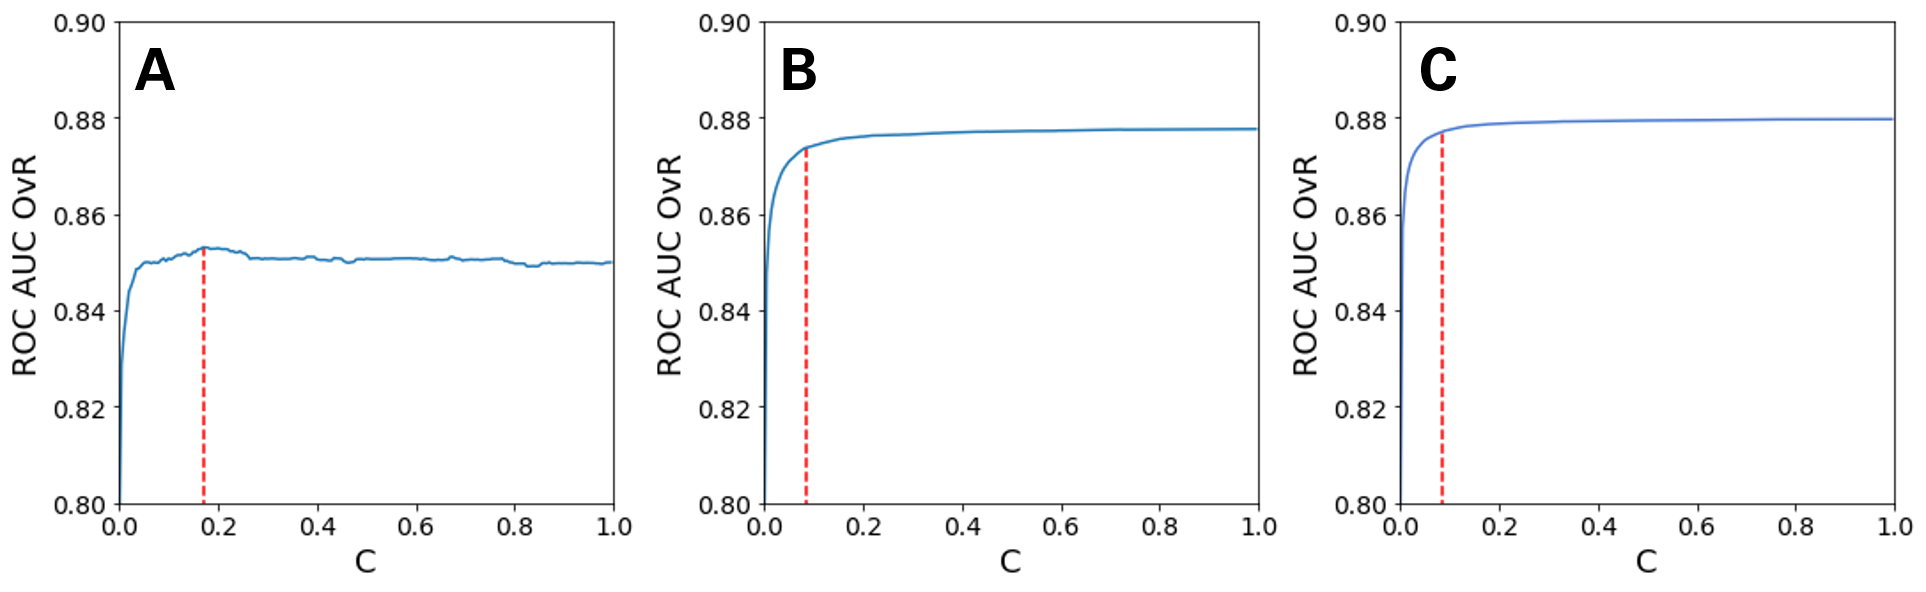
\includegraphics[width=\textwidth]{templates/images/Figure-LR_C_tuning.png}
\singlespacing
\caption[Logistic regression hyperparameter tuning]{Tuning plots for logistic regression C hyperparameter based on ROC AUC OvR values for A. WDS  B. WDS4 C. WDS8. WDS value selected from the plot maximum. Selections for WDS4 and WDS8 target the elbow of the curve.}
\label{fig:logreg_hp_tuning}
\end{figure}

The training and validation subsets defined in Section \ref{ch3:strat_sample} were re-combined, then stratified sampled as part of a 10-fold cross-validation process. ROC AUC OvR was used as the scoring metric. In some circumstances, a clear maximum can appear in cross-validation results indicating the best parameter choice, as is the case for WDS. For WDS4 and WDS8, AUC values continue to increase as C increases, but the slope of the AUC-C curve levels off to form a corner or “elbow” in the plot (Figure \ref{fig:logreg_hp_tuning}). Selecting a C value in this corner balances the trade-off between overfitting the training data with too little regularization and underfitting from too much regularization. The chosen C values for WDS, WDS4, and WDS8 are listed in Table \ref{tab:logreg_tuning}.

AUC values calculated on test subsets indicate WDS4 has the best out-of-sample performance of the three data sets. Figure \ref{fig:logreg_coefs} shows a plot of the feature coefficients for each of the one-vs-rest classifiers based on WDS4. Longer bars indicate larger influence on the model prediction. The top 5 features across the four classifiers are Si Geothermometer Temperature, Basement Depth, Drainage Density, Spring Density, and Volcanic Dike Density.

\begin{figure}[!htp]
\centering
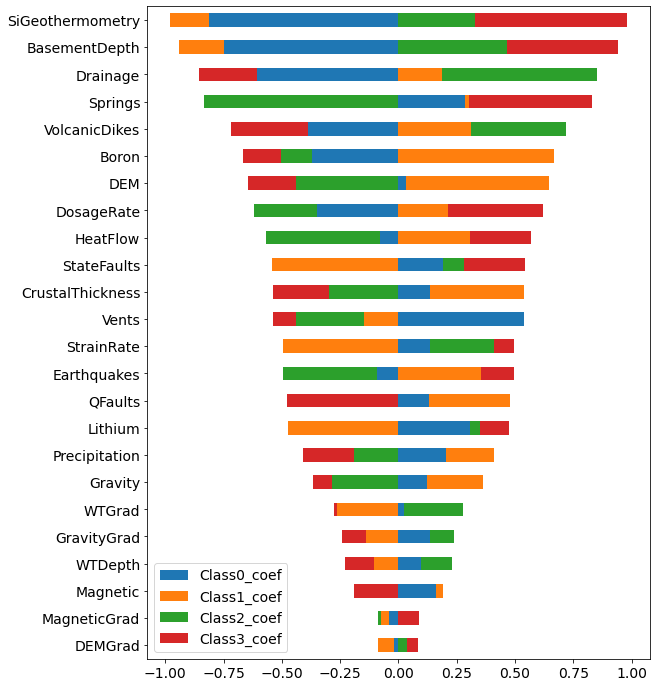
\includegraphics[width=\textwidth]{templates/images/Figure-LR-coefficients.png}
\singlespacing
\caption[Logistic regression feature coefficients]{Logistic regression coefficient values for OvR classifiers trained on WDS4.Stacked bar length is a proxy for overall importance to the classification.}
\label{fig:logreg_coefs}
\end{figure}

\subsubsection{Recursive Feature Elimination}
Logistic regression models assume a linear relationship between predictors and the response variable, but adding more predictors will not necessarily improve the model. Feature selection can lead to simpler models with the same predictive power but reduced risk of collinearity, which is important when managing data from naturally integrated earth systems. 

One method for selecting the number of features to keep involves an iterative process called \acrlong{rfe} (\acrshort{rfe}) (Brownlee, 2020c; scikit-learn, 2021d). The concept is relatively simple: RFE recursively selects and removes the feature with the smallest coefficient in the logistic regression model, then refits the data and repeats until a user-defined number of features is reached.  A plot of AUC vs. number of features can be constructed by looping over different feature limits, where the logistic regression model is fit on the training subset and evaluated on the validation subset (Figure \ref{fig:logreg_rfe}). Based on the plot, a local peak in AUC occurs when 18 features are used. Adding the remaining features results in small gains in AUC, but with diminishing returns for six additional features of complexity. Using this threshold, the data layers removed from the model include: DEM Gradient, Gravity Gradient, Magnetic Anomaly, Magnetic Anomaly Gradient, Water Table Depth, and Average Precipitation. Note that Average Precipitation appears higher on the coefficients plot (Figure \ref{fig:logreg_coefs}) than other features that were not removed. Since RFE iteratively removes predictors and refits the model, relative coefficients can change, particularly if there was collinearity with a removed variable.

\begin{figure}[!htp]
\centering
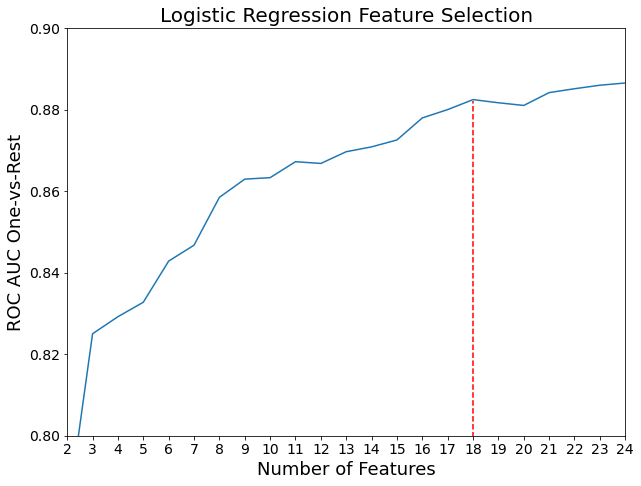
\includegraphics[width=0.6\textwidth]{templates/images/Figure-LR_feature_selection.png}
\singlespacing
\caption[Logistic regression feature selection]{Logistic regression feature selection using RFE and WDS4. Red dashed line indicates the chosen number of features to use for the LR model.}
\label{fig:logreg_rfe}
\end{figure}
\subsubsection{Optimized Model Results}\label{ch5:logreg_results}

\begin{wrapfigure}{R}{0.50\linewidth}
\centering
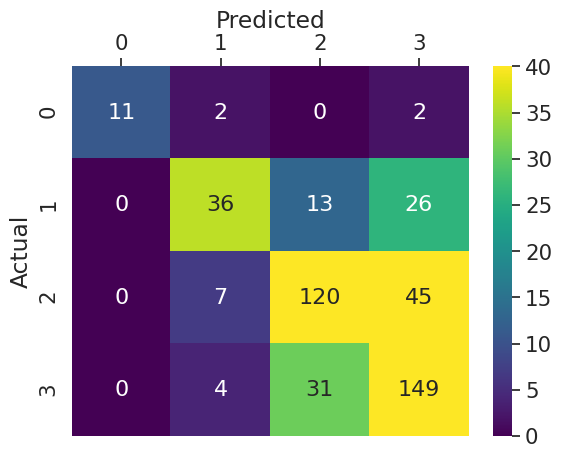
\includegraphics[width=0.45\textwidth]{templates/images/Figure-LR-ConfusionMatrix.png}
\singlespacing
\caption[Logistic regression confusion matrix]{Confusion matrix for the tuned LR model trained on WDS4.}
\label{fig:logreg_conf_matrix}
\end{wrapfigure}
A final LR model trained on WDS4 was constructed using the tuned C hyperparameter and reduced feature set from RFE. The confusion matrix suggests the model performs well overall (Figure \ref{fig:logreg_conf_matrix}). Correct predictions for all four classes of geothermal gradient (TP) outnumber the mis-classifications for those classes (FP). The model appears to struggle most with differentiating between class 2 and class 3 locations, which separate mid-grade (40-60 $^\circ$C/km) from high-grade gradients (>60 $^\circ$C/km), although there are a large number of mis-classifications (26) of low-grade gradient as high-grade as well.

Figure \ref{fig:logreg_auc} plots the macro average, micro average, and individual class ROC curves. Class 0 (non-thermal) predictive ability is quite high, pulling the micro-average AUC up to 0.88.  The macro AUC value of 0.85 is more aligned with the performance for other classes, which range from an AUC of 0.79-0.83. The trade-off between Class 2 and Class 3 is apparent in how the curve shapes mirror each other.

\begin{figure}[!htp]
\centering
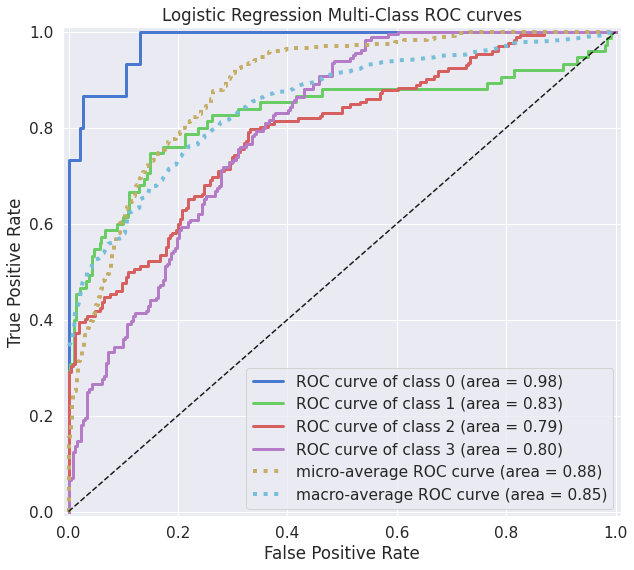
\includegraphics[width=0.6\textwidth]{templates/images/Figure-LR-AUC.png}
\singlespacing
\caption[Logistic regression AUC curves]{ROC AUC curves for the tuned LR model trained on WDS4.}
\label{fig:logreg_auc}
\end{figure}

Model predictions for the study area are generated by passing the FDS through the final trained model. Class predictions are plotted in Figure \ref{fig:logreg_final_map}. High-grade geothermal gradient patches are concentrated to the southeast and through the center of the AOI. Smaller high-grade regions are observed along the southwest state boundary, following the Rio Grande River to the northeast, and a smaller patch directly to the north.  Comparing this result to the data layer from \citet{bielicki_hydrogeolgic_2015}, high-grade predictions match in general spatial location except for the predicted patches to the north. The logistic regression model tends to predict more pervasive high geothermal gradients, and under-predicts the lower gradient regions to the north, east, and mid-AOI near the Rio Grande compared to the PFA layer.

\begin{figure}[!htp]
\centering
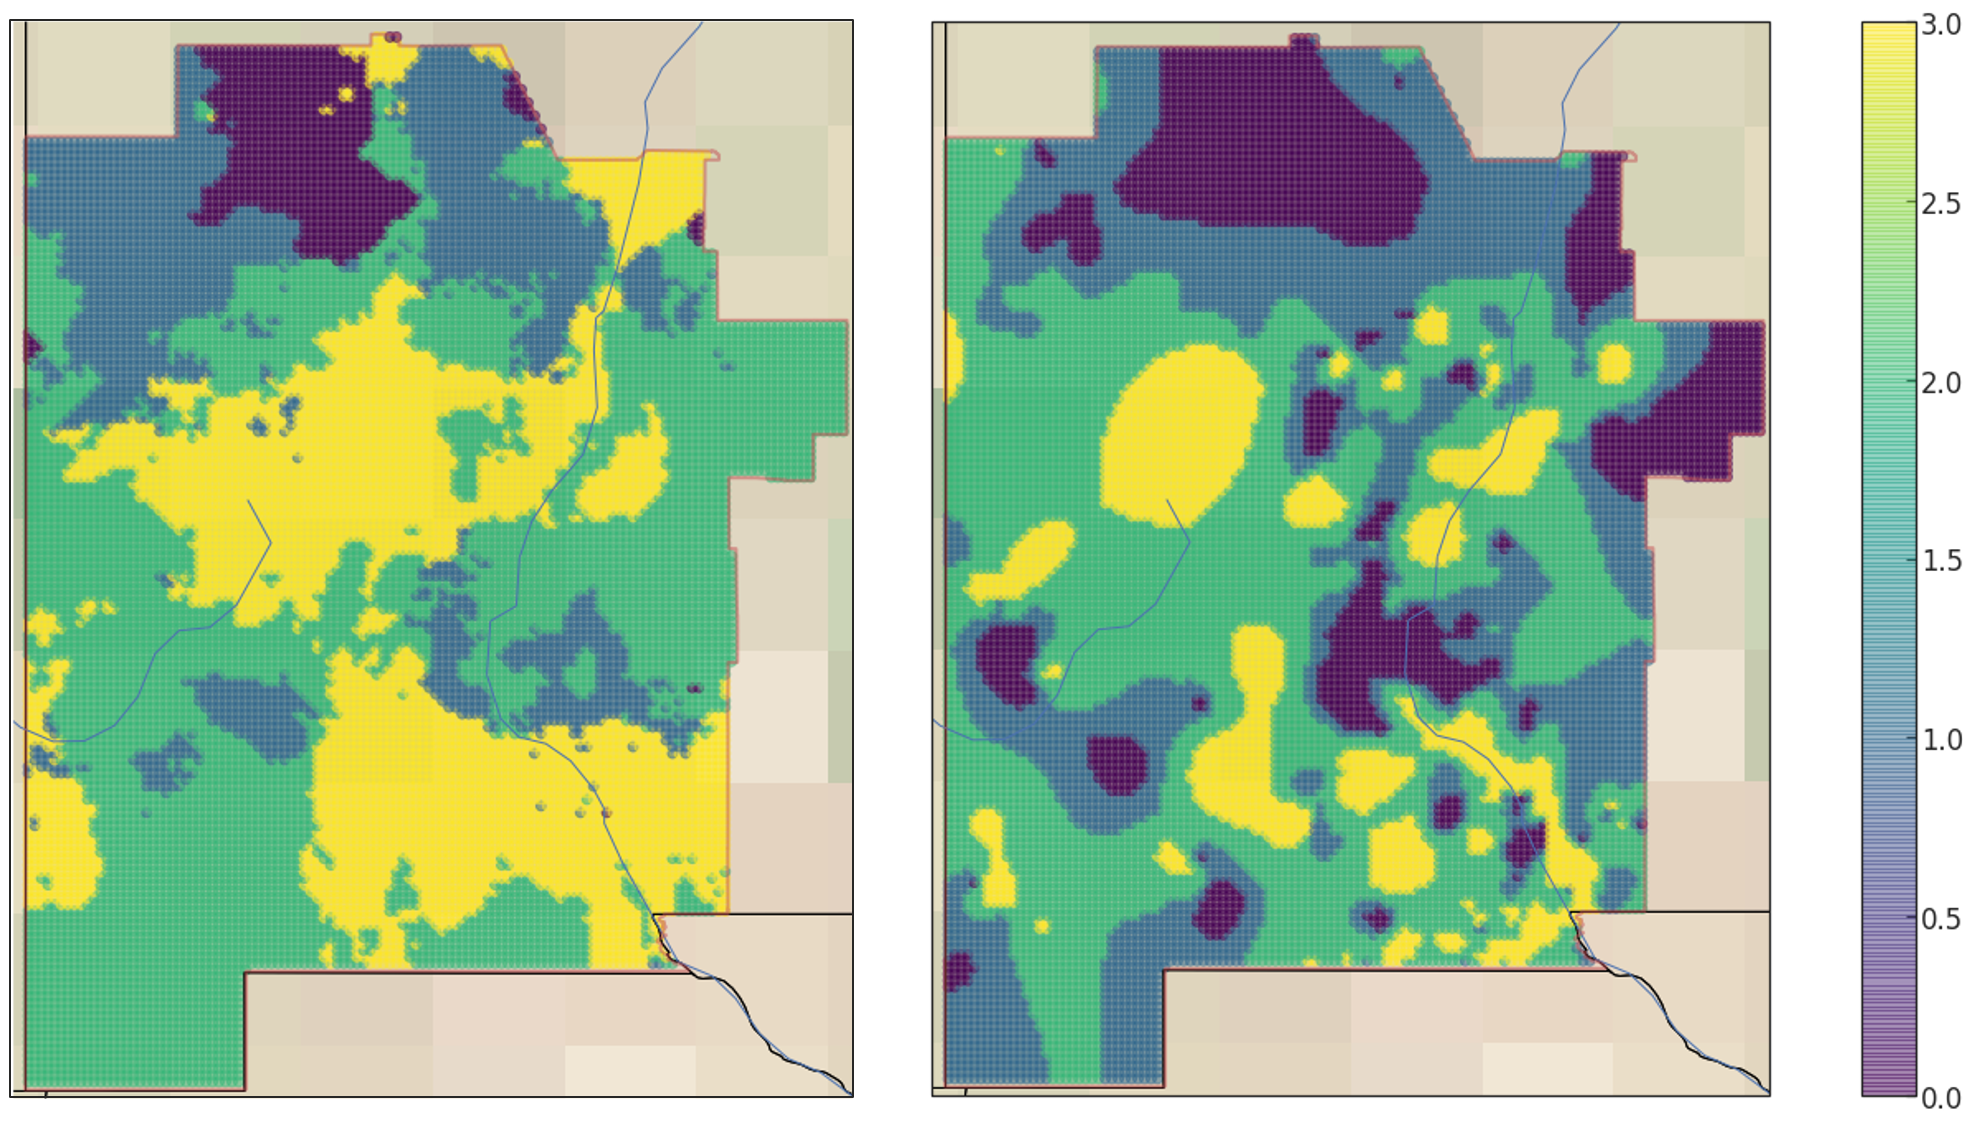
\includegraphics[width=\textwidth]{templates/images/Figure-LR-FinalMap_Joint.png}
\caption[Logistic regression prediction map]{Left: Map predictions of geothermal gradient class from the tuned LR model trained on WDS4. Right: geothermal gradient data layer from southwestern NM PFA study \protect\citep{bielicki_hydrogeolgic_2015}.}
\label{fig:logreg_final_map}
\end{figure}

\subsection{Decision Trees}\label{ch5:decision_trees}
 
A decision tree, sometimes known as a Classification and Regression Tree (CART), classifies observations using a cascading set of evaluations, each on individual predictor variables. There is no assumption of a linear response in the system. In fact, decision trees are uniquely suited to representing non-linear behavior in a highly-explainable way; once constructed, the decision tree describes a flowchart-like roadmap for each label assignment \citep[~p. 373-375]{bertsimas_analytics_2016}. Not every predictor will necessarily appear in the decision tree --- only those found to be significant during tree construction. And the most significant variables tend to be associated with early decision splits, placing them higher in the tree \citep[~p. 376]{bertsimas_analytics_2016}. Because of this, decision trees naturally provide insights into feature importance. 

\subsubsection{Tree Construction}
Decision trees are constructed by recursively performing binary splits on the training data set. Each split defines two new nodes in the tree, which correspondingly separates a group within the training data into subgroups. These subgroups represent child paths from the split node that terminate in two new terminal leaf nodes on the tree. The classification decision for each leaf will be the most commonly occurring class from the training data observations that are assigned to that leaf \citep[~p. 311]{james_introduction_2013}.

There are three metrics that can play a role in evaluating the discriminating quality of a particular decision node on the tree:

\begin{itemize}
    \item \textbf{Classification error rate}: the proportion of training samples that do not match the dominant class associated with a leaf node \citep[~p. 312]{james_introduction_2013}.
    \begin{equation} \label{eq:error_rate}
        E = 1 - \max_k(\hat{p}_{mk})
    \end{equation}
    where $m$ is the segment of the data associated with a node, $k$ is the class, and $\hat{p}_{mk}$ is the fraction of all training observations in $m$ that are of class $k$. 
    \item \textbf{Gini index}: measures variance across all k classes. Gini is sometimes known as a purity measurement because low values correspond with a strongly dominant class \citep[~p. 312]{james_introduction_2013}.
    \begin{equation}
        G = \sum_{k=1}^{K}{\hat{p}_{mk}(1-\hat{p}_{mk})}
    \end{equation}
    \item \textbf{Entropy}: An alternative form of purity measure, which also shows low values when the proportion of one class dominates the others within a node \citep[~p. 312]{james_introduction_2013}.
    \begin{equation}
        D = -\sum_{k=1}^{K}{\hat{p}_{mk}* \text{log}(\hat{p}_{mk})}
    \end{equation}
\end{itemize}

The purity aspect of both Gini index and entropy make them good choices for tree construction. In the forward pass, the tree will iteratively grow by selecting nodes in the tree, a predictor to split on, and a threshold value defining the split. These choices are optimized by the chosen quality metric. The tree will grow until a stopping condition is met, like reaching a maximum tree depth or minimum number of observations allowed per node. Tree clean-up then takes place in a backward pass, where the following decision tree objective governs whether a tree branch is kept or removed \citep[~p. 309]{james_introduction_2013}:

\begin{equation}
\min{\{SSE + \alpha\left|T\right|\}} = \min\Bigg\{ \sum_{m=1}^{\left|T\right|}{\sum_{i|x_i\epsilon R_m}}{(y_i-\hat{y}_m)^2+ \alpha\left|T\right|\Bigg\}}
\end{equation}

Here, $\left|T\right|$ refers to the number of terminal nodes in tree $T$, $R_m$ is the subgroup of the training data associated with terminal node $m$, and $\hat{y}_m$ is the classification predicted by node $m$. If the sum of squared errors ($SSE$) in classification increases by less than $\alpha$ when a branch is removed, that branch will remain removed from the decision tree. $\alpha$ acts as a regularization parameter balancing prediction accuracy with model complexity; greater values of $\alpha$ result in simpler decision trees.

\subsubsection{Hyperparameter Tuning}
Multiple hyperparameters determine the performance of a decision tree classifier. Here we consider six parameters, each of which are tuned using the Stratified k-Fold CV method described in Section \ref{ch5:strat_kfold_cv}, with 10 folds and the multi-class one-vs-rest ROC AUC as the scoring metric. The figure examples illustrate the tuning procedure for WDS4.

First, \verb|max_depth| and \verb|criterion| were tuned together. \verb|max_depth| limits tree expansion by capping the number of parameter evaluations (tree nodes) considered before a classification label assignment. \verb|criterion| refers to the quality metrics defined above. Figure \ref{fig:dtree_maxdepth} illustrates the relative insensitivity the classifier has to \verb|criterion|, while tree depth plays a stronger role in performance. A maximum AUC score is observed with a \verb|max_depth| of 8 and \verb|criterion| choice of Entropy.

\begin{figure}[!htp]
\centering
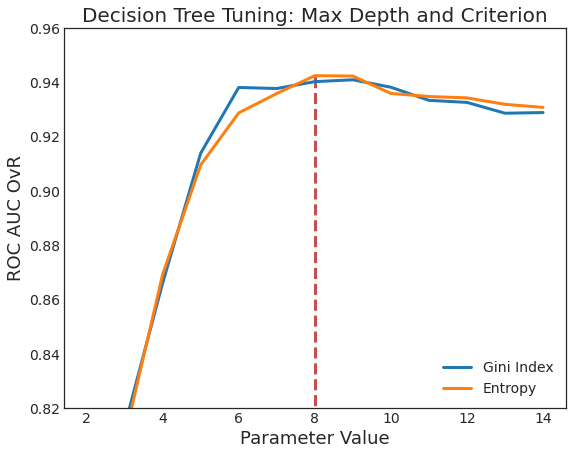
\includegraphics[width=.6\textwidth]{templates/images/Figure-DT_tuning_maxdepth_criterion.png}
\caption[Decision tree max depth tuning]{Results from stratified k-fold cross validation tuning of max\_depth and criterion hyperparameters using WDS4. The red dashed line indicates the selected max\_depth value.}
\label{fig:dtree_maxdepth}
\end{figure}

Next, \verb|min_samples_leaf| and \verb|min_samples_split| were tuned in succession. The former defines the minimum number of samples from the training set that must be assigned to a leaf node for that leaf to remain in the tree. The latter sets a minimum number of training set samples that must be assigned to a node before that node can be considered for a split. Figure \ref{fig:dtree_min_samples} illustrates the selected parameter values, defined by maxima in the AUC vs. parameter value plots. The insensitivity of the classifier to low values of \verb|min_samples_split| illustrates the cascading influence of the hyperparameters in this tuning flow. When \verb|min_samples_leaf| is set to 8, a split can only occur when the node being split has at least 16 observations, so any \verb|min_samples_split| value under 16 does not influence tree construction. 

\begin{figure}[!htp]
\centering
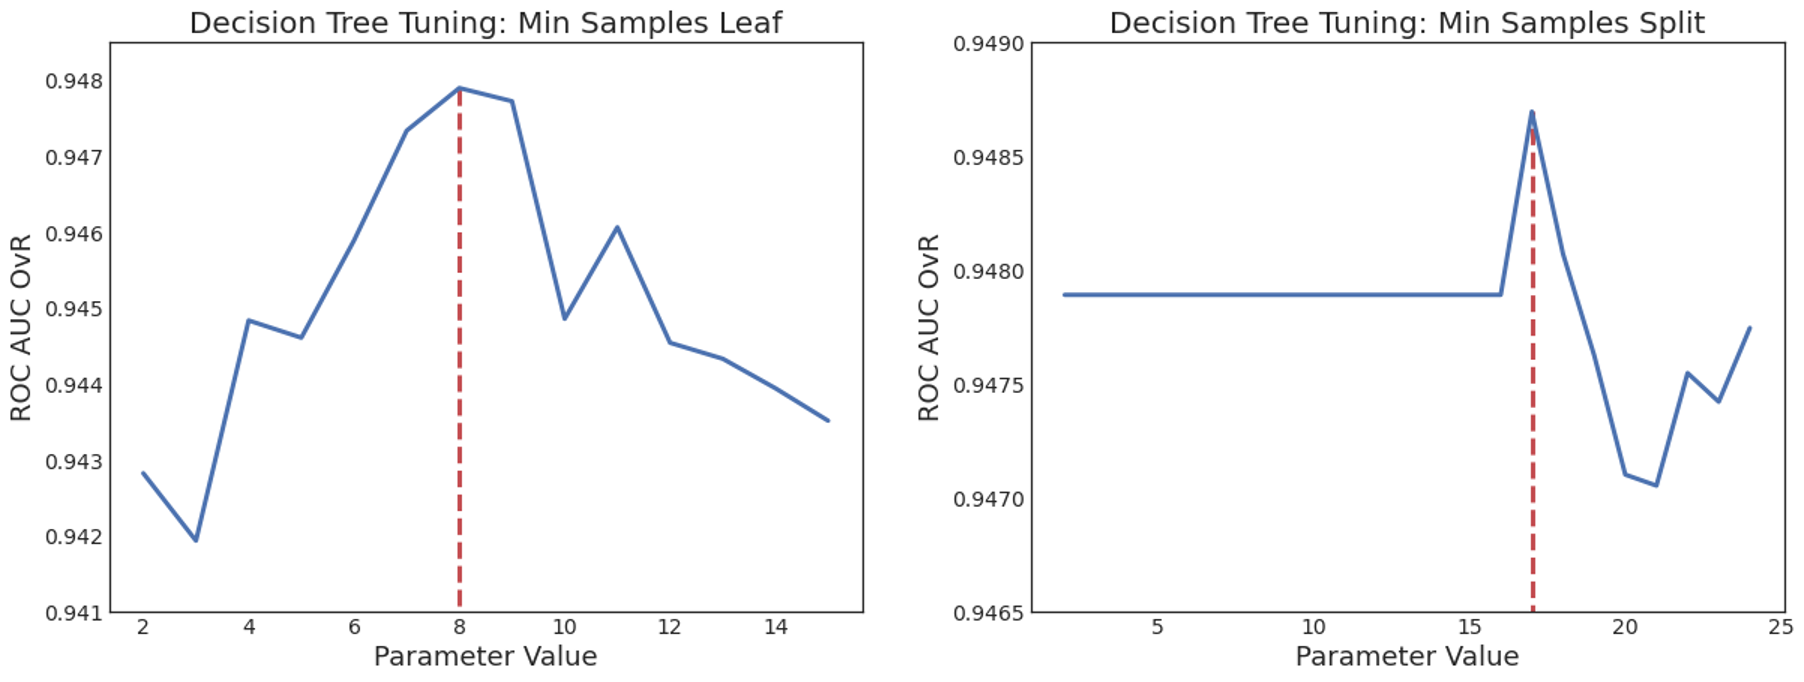
\includegraphics[width=\textwidth]{templates/images/Figure-DT_tuning_min_samp_leaf_split.png}
\caption[Decision tree min samples tuning]{Results from stratified k-fold cross validation tuning of min\_samples\_leaf (Left) and min\_samples\_split (Right) hyperparameters using WDS4. The red dashed lines indicate the selected values.}
\label{fig:dtree_min_samples}
\end{figure}

One optimization trick is to only consider a subset of the features when splitting decision tree nodes. This also adds an element of randomness to tree construction, so decision trees can differ when constructed on the same training data depending on how many features were considered for each split. No clear maximum appears in the AUC plot for \verb|max_features| (Figure \ref{fig:dtree_max_features}), so a value of 8 was selected using the elbow criterion described in Section \ref{ch5:hyper_tuning}. \verb|max_features| can also cause problems when performing feature selection if the feature count drops  below the \verb|max_features| value, so care must be taken in using this parameter.

\begin{figure}[!htp]
\centering
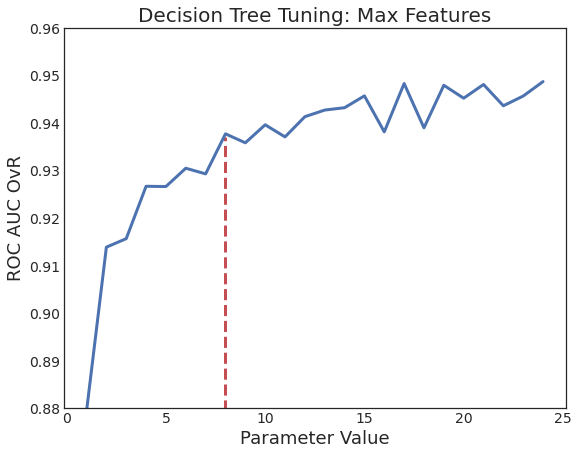
\includegraphics[width=.6\textwidth]{templates/images/Figure-DT_tuning_max_features.png}
\caption[Decision tree max features tuning]{Results from stratified k-fold cross validation tuning of max\_features parameter using WDS4. The red dashed line indicates the selected value, selected in the “elbow” of the plot.}
\label{fig:dtree_max_features}
\end{figure}

The final parameter, \verb|ccp_alpha|, controls the trade-off between model fit and complexity during the tree pruning backward pass of tree construction. As the alpha value increases from zero, the difference between in-sample (training) and out-of-sample (validate) performance decreases, but so does the overall performance of the classifier on the validation subset. Figure \ref{fig:dtree_alpha} shows a clear minima in train-validate AUC difference, however the validation set performance drops from 0.95 to under 0.85 when using this value for \verb|ccp_alpha|. The default value of \verb|ccp_alpha| = 0.0 is chosen instead.

\begin{figure}[!htp]
\centering
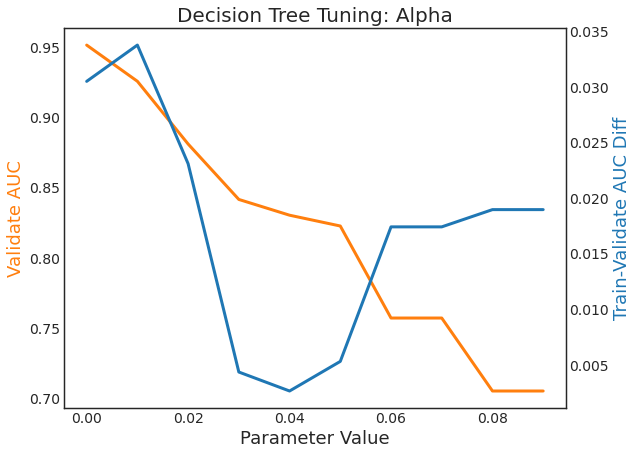
\includegraphics[width=.6\textwidth]{templates/images/Figure-DT_tuning_alpha.png}
\caption[Decision tree alpha tuning]{Results from stratified k-fold cross validation tuning of the ccp\_alpha parameter. The orange line plots the validation subset AUC. The blue line plots the difference in AUC between training and validation subsets.}
\label{fig:dtree_alpha}
\end{figure}

Final hyperparameter values and performance results for WDS, WDS4, and WDS8 are listed in Table \ref{tab:dtree_tuning}. Data augmentation results in a significant improvement in classifier performance over the original WDS.

\begin{table}[!htp]
\centering
\begin{tabular}{c|c|c|c|}
\cline{2-4}
                                          & WDS & WDS4 & WDS8 \\ \hline
\multicolumn{1}{|c|}{criterion}           & Gini & Entropy & Entropy \\ \hline
\multicolumn{1}{|c|}{max\_depth}          & 5 & 8 & 10 \\ \hline
\multicolumn{1}{|c|}{min\_samples\_leaf}  & 7 & 8 & 10 \\ \hline
\multicolumn{1}{|c|}{min\_samples\_split} & 21 & 17 & 24 \\ \hline
\multicolumn{1}{|c|}{max\_features}       & 5 & 8 & 6 \\ \hline
\multicolumn{1}{|c|}{ccp\_alpha}          & 0  & 0 & 0 \\ \hline
\multicolumn{1}{|c|}{AUC$_{train}$}       & 0.89 & 0.97 & 0.99 \\ \hline
\multicolumn{1}{|c|}{AUC$_{test}$} & 0.82 & 0.95 & 0.96 \\ \hline
\end{tabular}
\caption[Decision tree hyperparameter values]{Tuned hyperparameter selections and resulting model AUC for training and test subsets of WDS, WDS4, and WDS8.}
\label{tab:dtree_tuning}
\end{table}

Figure \ref{fig:dtree_feat_import} shows the feature importances determined by the decision trees for WDS, WDS4, and WDS8.  Features are sorted on the sum importance value across all 3 data sets. Although differences exist, Si Geothermometer Temperature appears as the most important predictor in all cases. And the bottom six features are also remarkably consistent across the data sets: Water Table Depth, Water Table Gradient, Gravity Anomaly Gradient, Magnetic Anomaly, Magnetic Anomaly Gradient, and DEM Gradient. Dropping these features reduces the overall decision tree data set to 18 features total.

\begin{figure}[!htp]
\centering
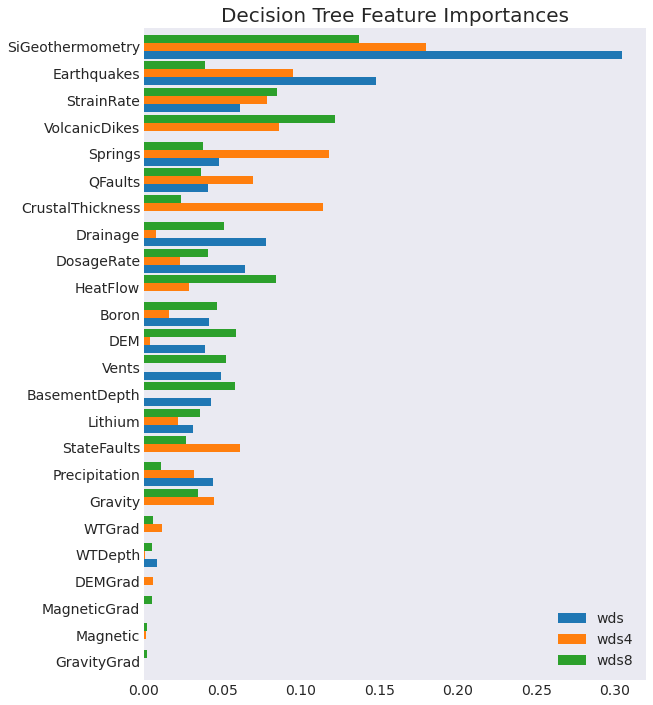
\includegraphics[width=\textwidth]{templates/images/Figure-DT_feature_importances_all.png}
\caption[Decision tree feature importances]{Decision tree feature importances for WDS, WDS4, and WDS8, sorted on the sum total importance across the 3 data sets.}
\label{fig:dtree_feat_import}
\end{figure}

\subsubsection{Optimized Model Results}
\begin{figure}[!htp]
\centering
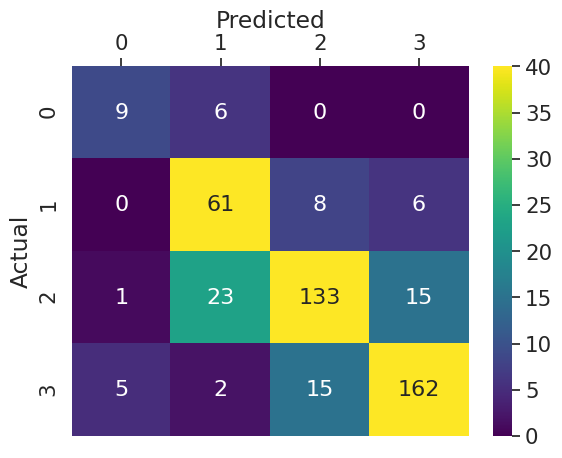
\includegraphics[width=0.45\textwidth]{templates/images/Figure-DT-ConfusionMatrix.png}
\singlespacing
\caption[Decision tree confusion matrix]{Confusion matrix for tuned DT model trained on WDS4.}
\label{fig:dtree_conf_matrix}
\end{figure}
A final DT model trained on WDS4 was constructed using the tuned parameters and 18-predictor reduced feature set. The confusion matrix (Figure \ref{fig:dtree_conf_matrix}) demonstrates an improvement in model results over the logistic regression method. Low-grade geothermal locations are correctly predicted for almost double the number of sites, and half as many mis-classifications are observed between class 2 (mid-grade) and class 3 (high-grade) geothermal as with the LR model.

Figure \ref{fig:dtree_auc} shows the macro average, micro average, and individual class DT ROC curves. All individual class AUC values exceed 0.90. Class 0 (non-geothermal) continues to demonstrate the highest predictive ability (AUC=0.97), but the performance of class 3 (high-grade) is most responsible for boosting micro-average AUC at higher decision thresholds where the class 0 ROC curve steeply drops in TPR for FPR < 0.1. Class 2 (medium-grade) classification performance lags behind the other classes for the DT classifier.

\begin{figure}[!htp]
\centering
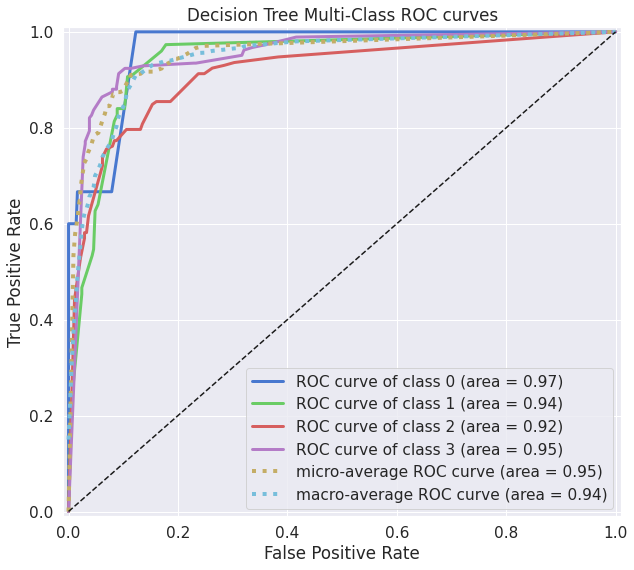
\includegraphics[width=0.6\textwidth]{templates/images/Figure-DT_AUC.png}
\caption[Decision tree AUC curves]{ROC AUC curves for the tuned DT model trained on WDS4.}
\label{fig:dtree_auc}
\end{figure}

Model predictions for the study area are generated by passing the FDS through the DT model. Class predictions based on the OvR methodology are plotted in Figure \ref{fig:dtree_final_map}. The high-grade geothermal gradient patches to the southeast and central regions of the AOI are smaller in areal extent and more disconnected than for the LR model (Figure \ref{fig:logreg_final_map}). Predictions for low or no-gradient are concentrated to the NW in the CP province, central-east where RGR transitions into the Great Plains, and south in the southern BR province. The overall distribution of geothermal gradient classes matches the \citet{bielicki_hydrogeolgic_2015} PFA layer (Figure \ref{fig:dtree_final_map}) with a greater distribution of high-gradient locations and fewer low/no-gradient ones.

\begin{figure}[!htp]
\centering
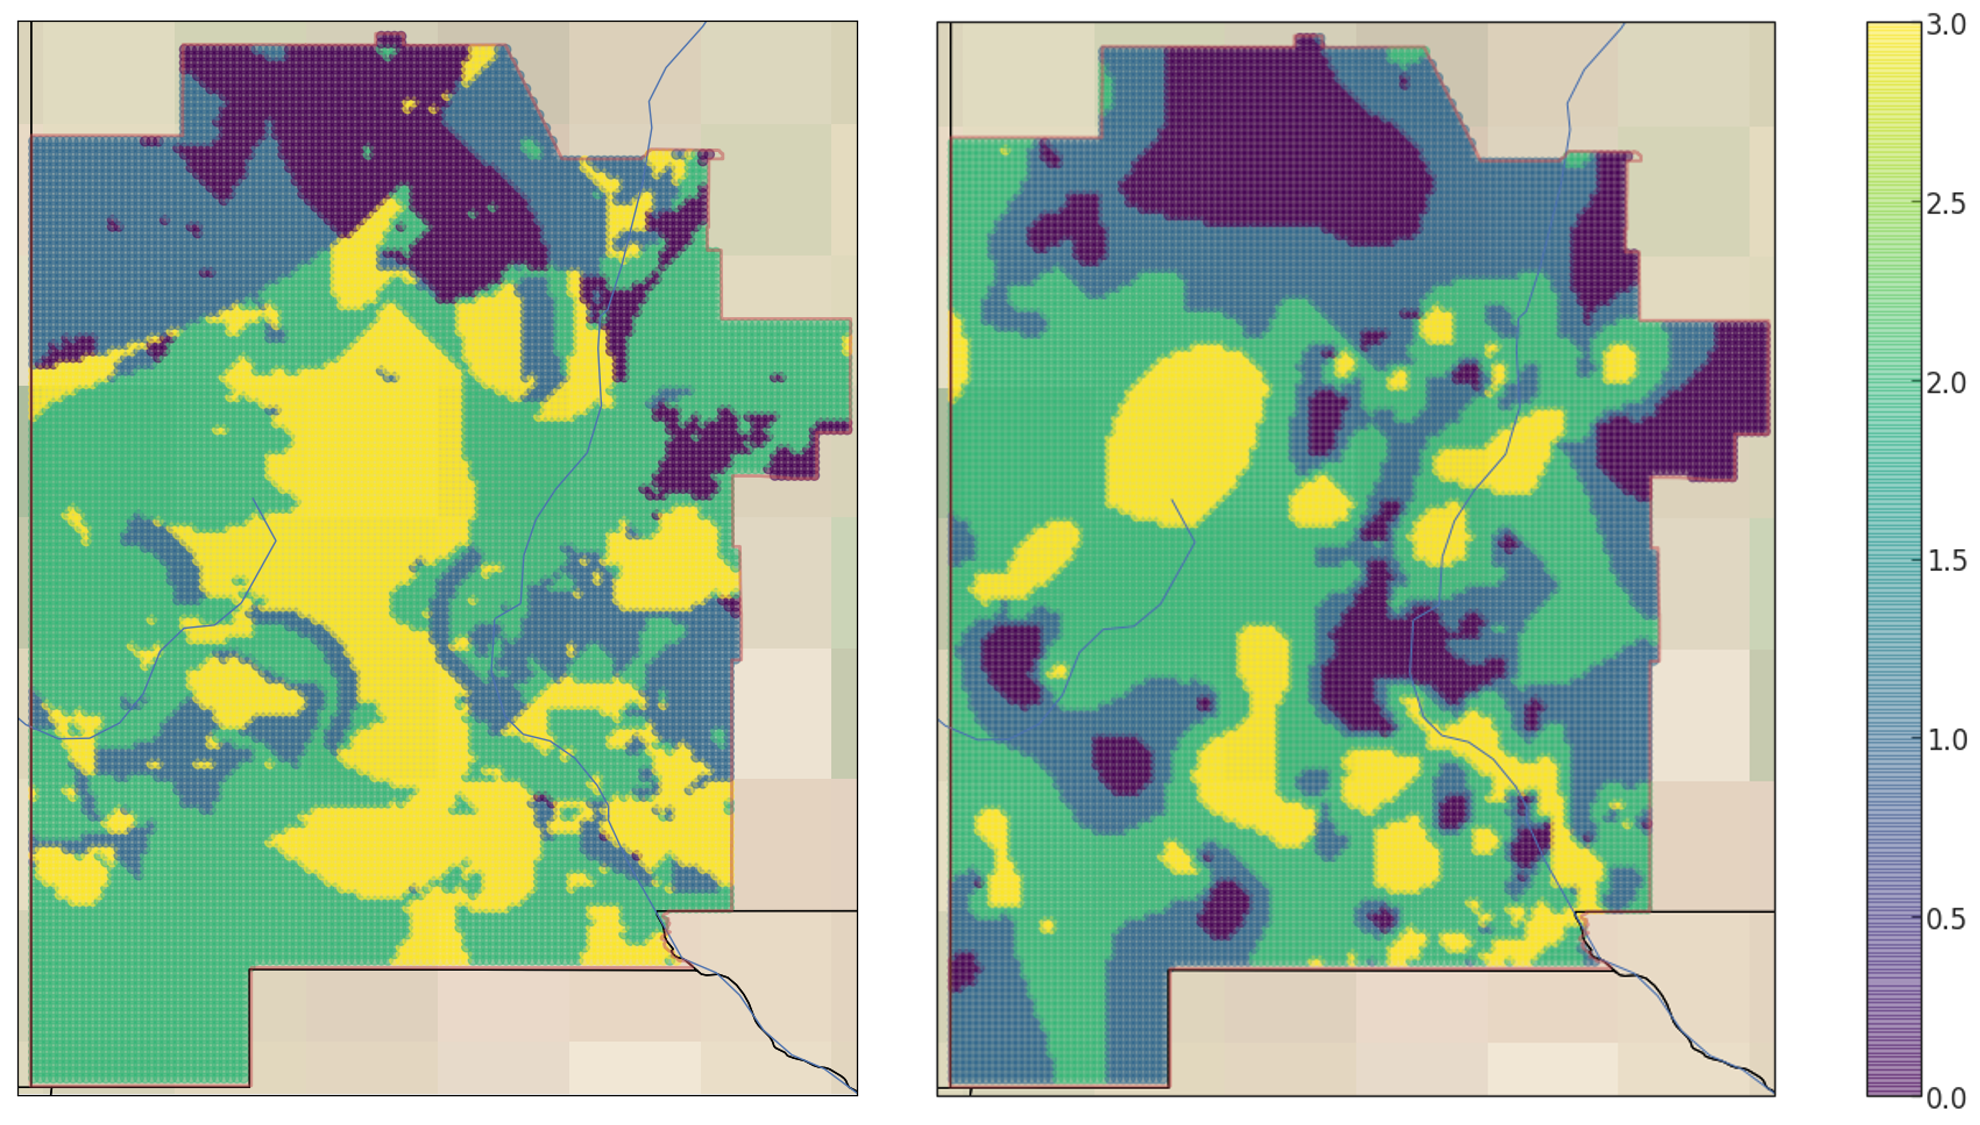
\includegraphics[width=\textwidth]{templates/images/Figure-DT-FinalMap_Joint.png}
\caption[Decision tree prediction map]{Left: Map predictions of geothermal gradient class from the tuned DT model trained on WDS4. Right: geothermal gradient data layer from southwestern NM PFA study \protect\citep{bielicki_hydrogeolgic_2015}}
\label{fig:dtree_final_map}
\end{figure}

Interesting high-gradient patches appear to the southwest and northeast, one of which is surrounded by an unusually cohesive ring of class 0 non-thermal predictions. Note that when the random seed changes and a new decision tree is constructed, this ring typically goes away. In fact, one downside of the decision tree model is its unstable nature; decision trees can change each time the algorithm is run, even on the same training data, due to randomness in the node splitting process. Nevertheless, tree performance remains relatively stable overall. And the ability to plot and trace through the model makes it one of the most accessible and interpretable methods to use (See Figure \ref{fig:dtree_viz}).

\begin{figure}[!htp]
\centering
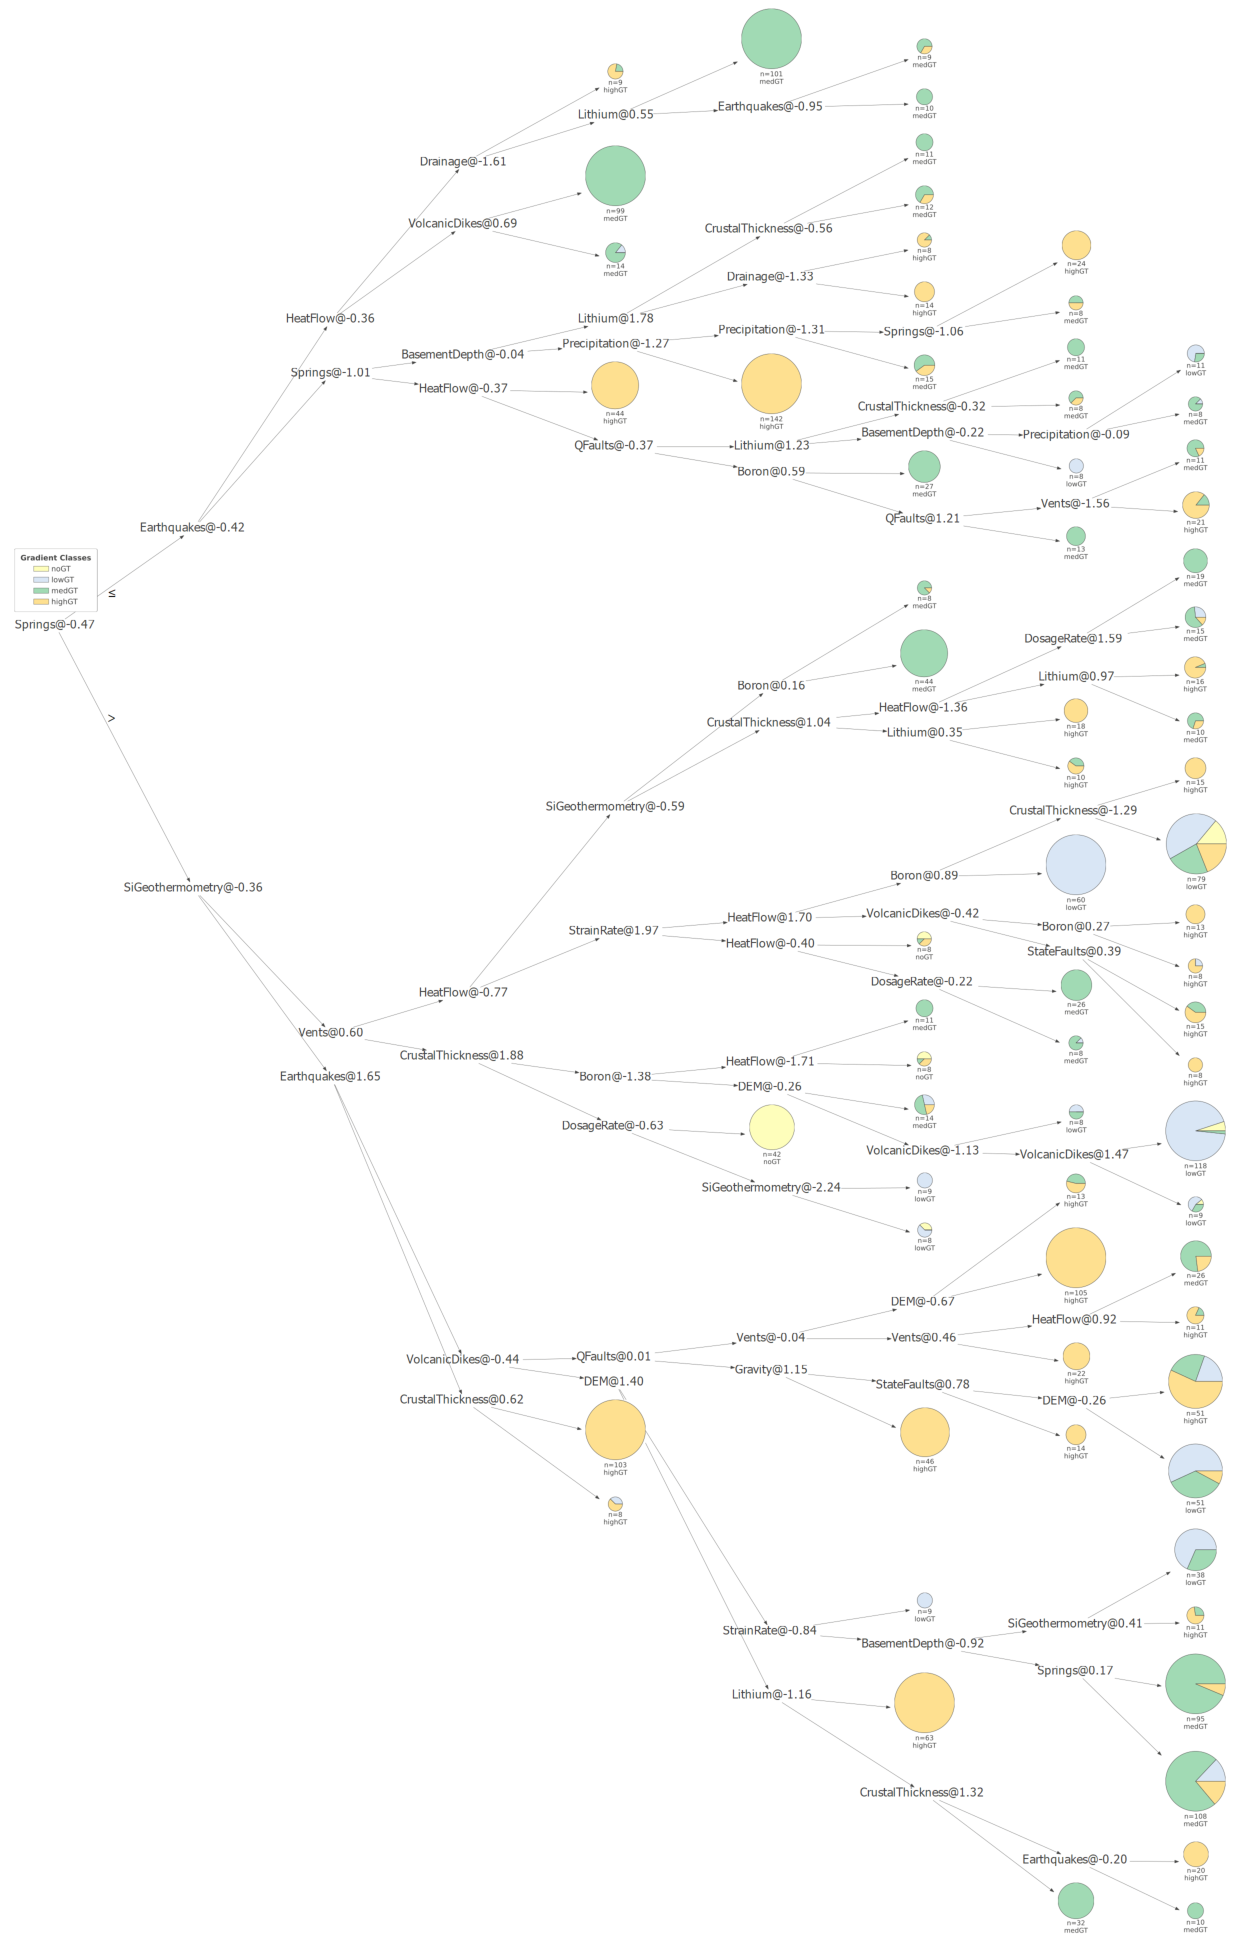
\includegraphics[height=0.9\textheight,keepaspectratio]{templates/images/Figure-DT_viz_portrait.pdf}
\caption[Decision tree visualization]{Decision tree visualization for the final decision tree model.Nodes are noted by predictor labels with their decision threshold. Bubbles illustrate the final distribution of classes in a leaf node, sized by number of observations. The majority class determines the classification label.}
\label{fig:dtree_viz}
\end{figure}

\subsection{Tree Ensembles}

\subsection{Neural Networks}

\subsection{Uncertainty Analysis}

\subsubsection{Bootstrap Estimation}

\subsubsection{Information Entropy}

\subsubsection{Bayesian Networks}

\chapter{EGS Power Plant Expansion\\Cost Model Results}\label{ch6:cm_results}

Chapter \ref{ch4:cm_prep} outlined the cost modeling strategy for a hypothetical 5 MW expansion project of the Lightning Dock power plant in Animas Valley, NM. This chapter reviews the results of the different model approaches, explores insights gained from those models, and describes how this approach mitigates risks associated with geothermal production.

\section{Static Model}
\label{ch6:static_mod}

\subsection{Model Selection}
\label{ch6:static_select}

Section \ref{ch4:cm_rev} described the use of brine effectiveness in the cost model for determining the power output of a binary cycle plant for a given production temperature and flow rate. This formulation provides a choice of how to manage the cost model mechanics due to a trade-off between plant capacity and flow rate for a given brine effectiveness (Equation \ref{eq:cm_rev}).

In addition, installation of the Lightning Dock expansion can take place over a variety of different deployment schedules due to the modularity of the system. Rather than drill ten wells and install five binary cycle plants all at once, delaying aspects of the installation can be financially beneficial and less of an initial risk for the project.

Figure \ref{fig:static_model_compare} shows the results for the pre-set capacity and pre-set flow rate static models for sixty (60) installation schedule permutations. The pre-set capacity model results in project losses of \$20 million or more for all tested installation options. On the other hand, the fixed flow-rate model only drops below \$0 NPV for a handful of project plans, achieving \$3.7 million NPV for the case marked with a red diamond where three (3) modules are installed up front and two (2) additional ones go live after a year of operation. Based on these results, all cost models used in the rest of this analysis apply a fixed flow rate per production well and derive the aggregate electricity generation numbers based on the temperature of the produced brine.

\begin{figure}[!htp]
\centering
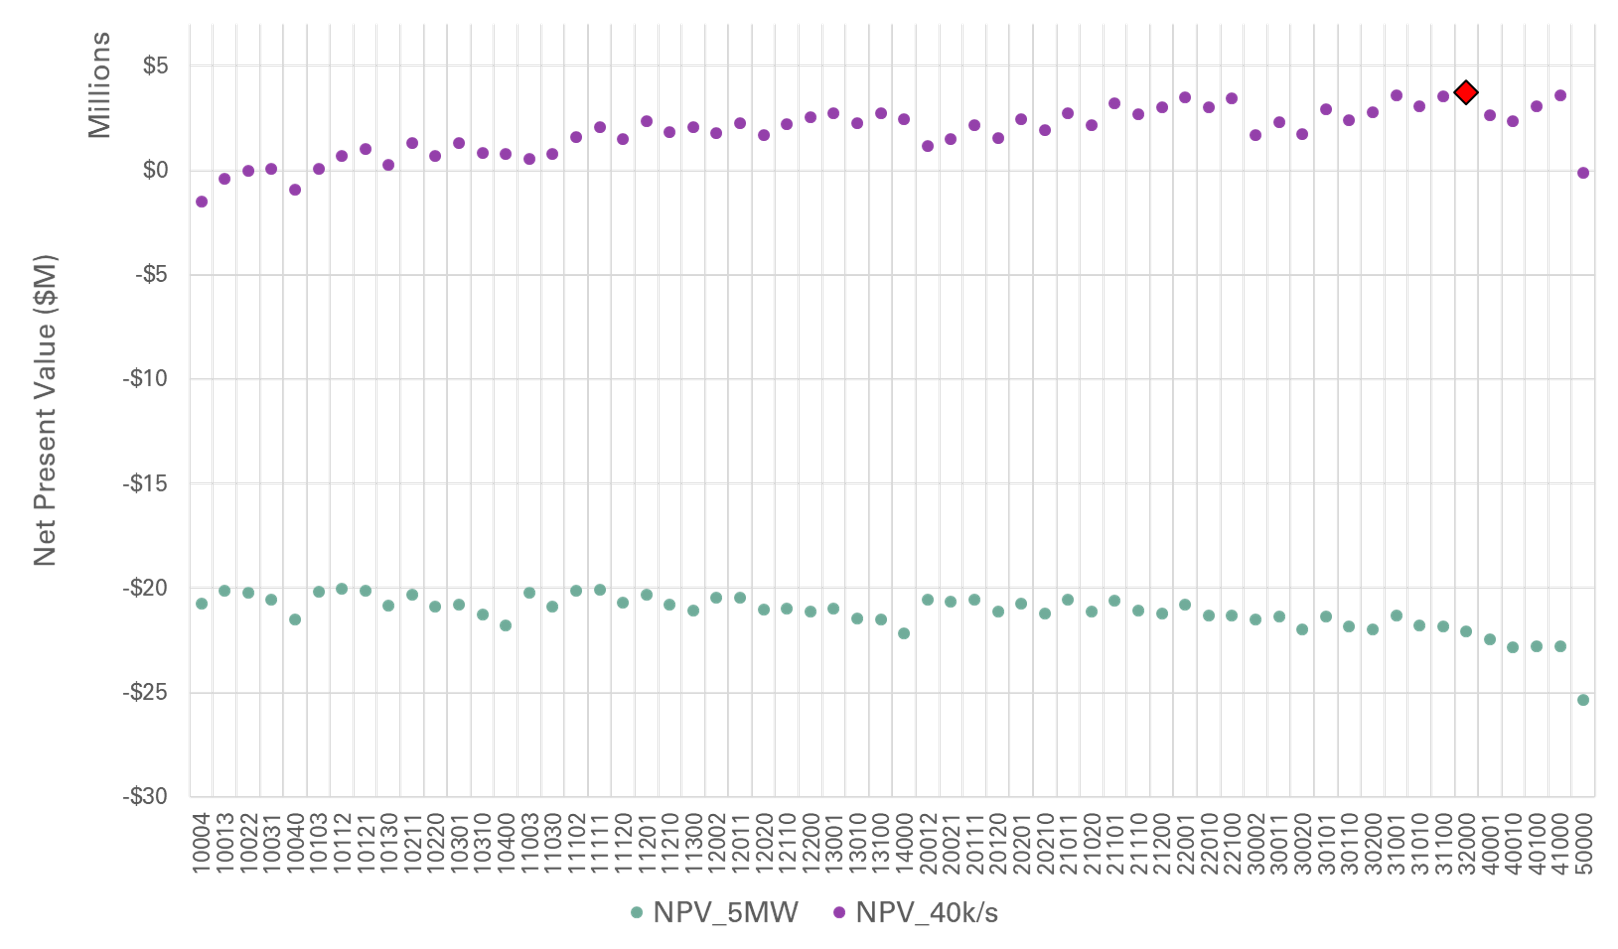
\includegraphics[width=.98\textwidth]
{templates/images/Figure-Static_Model_Construction.png}
\caption[Static cost model comparison]{Static cost model comparison between pre-set aggregate capacity (5 MW target, green) and pre-set flow rate per production well (40 kg/s, purple), plotted against module installation schedule. Both models deploy five modules in all schedule permutations involving up to a five-year period. The red diamond marks the optimal model and power plant expansion plan.}
\label{fig:static_model_compare}
\end{figure}

\subsection{Construction Optimization}
\label{ch6:static_schedule}

Lifting the fixed-capacity requirement changes the production potential for each power plant module. Based on the production parameters defined in Section \ref{ch4:cm_params}, each module can now generate 2.1 MW. Since this is a hypothetical case study with Climeon modules used as an analog only, further modeling uses this value with the caveat that future efforts confirm its viability as the modular power plant technology continues to evolve.

The updated power production per module reduces the required module count to a total of three (3) modules based on the original expansion target of $\approx$5 MW. Table \ref{tab:static_optimization} revisits the installation schedule grid search exercise to determine the optimal project plan under these circumstances. At an NPV of \$1.0 million, the best option deploys two (2) modules initially and adds an additional one (1) at the end of the first year. In order to standardize cost models for direct comparison, this installation plan is used for all cost models throughout the rest of this analysis.

\begin{table}[!htp]%{R}{0.4\linewidth}
\centering
\begin{tabular}{|c|c|c|c|}
\hline
\textbf{Year 0} & \textbf{Year 1} & \textbf{Year 2} & \textbf{NPV (\$M)} \\ \hline
3 & 0 & 0 & -\$1.1 \\ \hline
1 & 0 & 2 & -\$0.3 \\ \hline
1 & 1 & 1 & \$0.5 \\ \hline
1 & 2 & 0 & \$0.6 \\ \hline
2 & 0 & 1 & \$0.6 \\ \hline
2 & 1 & 0 & \$1.0 \\ \hline
\end{tabular}
\caption[Static model module installation schedule]{Grid search for the optimal power plant installation schedule based on the static cost model. Values are in \$M, where M is million.}
\label{tab:static_optimization}
\end{table}

\subsection{Summary Statistics}
\label{ch6:static_stats}

As a deterministic cost model, Static model performance is measured strictly on calculated NPV. This will act as a benchmark value for the other cost models explored in the rest of this chapter.

\begin{table}[H]
\centering
\begin{tabular}{|l|c|}
\hline
\textbf{Static Model Statistics} & \textbf{\$M} \\ \hline
NPV & \$1.0 \\ \hline
\end{tabular}
\caption[Static model statistics]{Static model statistics. NPV is reported in \$M, where M is million.}
\label{tab:static_mod_stats}
\end{table}

\section{Probabilistic Model Metrics}
\label{ch6:cost_model_metrics}

Monte Carlo simulation is applied to all of the probabilistic models to estimate the range of model behavior. For each model, results represent 2000 simulated runs where each realization defines a unique combination of variable values sampled from the PDFs reviewed in Section \ref{ch4:pdfs}. 

Common methods for evaluating a Monte Carlo ensemble include building a NPV histogram, constructing a \acrlong{cdf} (\acrshort{cdf} or target curve), and averaging the results together for \acrlong{enpv} (\acrshort{enpv}). Other interesting metrics for model comparison include standard deviation, individual percentiles, and direct comparison with the static model NPV (NPV$_{s}$). Standard deviation is the measure of how tightly the results cluster around the central value. Distributions with low standard deviations are sometimes referred to as robust distributions. P$_{50}$ marks the the median, and P$_{05}$ and P$_{95}$ define marginal percentiles for 5\% \acrlong{var} (\acrshort{var}) and \acrlong{vag} (\acrshort{vag}), respectively. Each of these measures is reported for the probabilistic model cases described below.

\section{Base Case Model}
\label{ch6:base_case}

The Base Case model mimics the Static model in form, but incorporates uncertainties in drilling \& completions costs, electricity pricing, geothermal gradient, reservoir temperature, and thermal drawdown rate to provide a more realistic forecast. No decision rules are included in this scenario. 

\subsection{Model Results}
\label{ch6:base_results}

At -\$4.8 million ENPV, the Base Case model predicts over 560\% lower project value than predicted with the Static model (Table \ref{tab:base_stats}). This result alone illustrates how probabilistic approaches can significantly differ from deterministic models that use most-likely or average values. Skewed system performance occurs even when variable distributions are balanced, which makes deterministic results both unrealistic and unreliable measures for decision-making \citep[p.\ 48-49]{de_neufville_flexibility_2011}. Here, unanticipated high-side (P$_{95}$ value of \$15.9 million) does exist, but the influence of the low-side (P$_{05}$ value of -\$28.2 million) dominates overall (Table \ref{tab:base_stats}).

The Base Case ensemble shows a symmetric, pseudo-Gaussian distribution of NPV results, with the exception of a long right tail capturing rare but very positive project outcomes (Figure \ref{fig:base_case_hist}). Figure \ref{fig:base_case_cdf} illustrates the target curve tracing cumulative probabilities for observed NPV values. The P$_{50}$ value of -\$3.9 million suggests the highly-negative values in the lower half of results pull the average (ENPV) further into negative project value territory. Cumulatively, $\approx60\%$ of the realizations end in a net loss for the project (Figure \ref{fig:base_case_cdf}). And at $\approx 3\times$ both the median and ENPV, standard deviation of NPV indicates this solution is not robust. 

\begin{figure}[!htp]
\centering
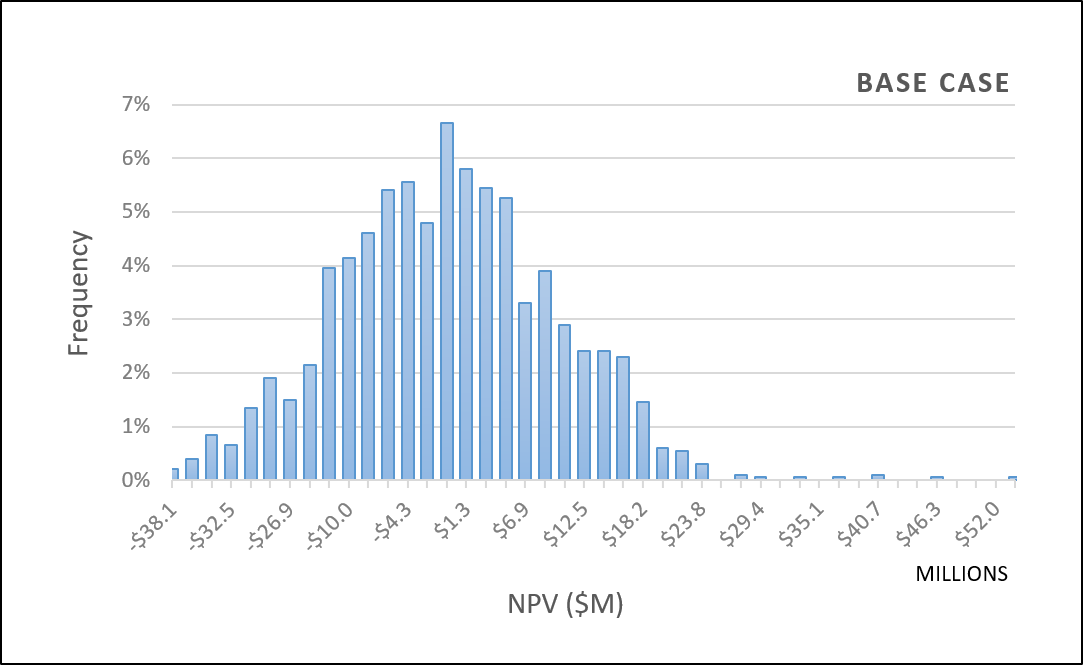
\includegraphics[width=.85\textwidth]{templates/images/Figure-Base_Case_Histogram.png}
\caption[Base Case histogram]{Base Case probabilistic cost model histogram illustrating the distribution of 2000 model realizations. NPV is reported in \$M, where M is million.}
\label{fig:base_case_hist}
\end{figure}

\begin{figure}[!htp]
\centering
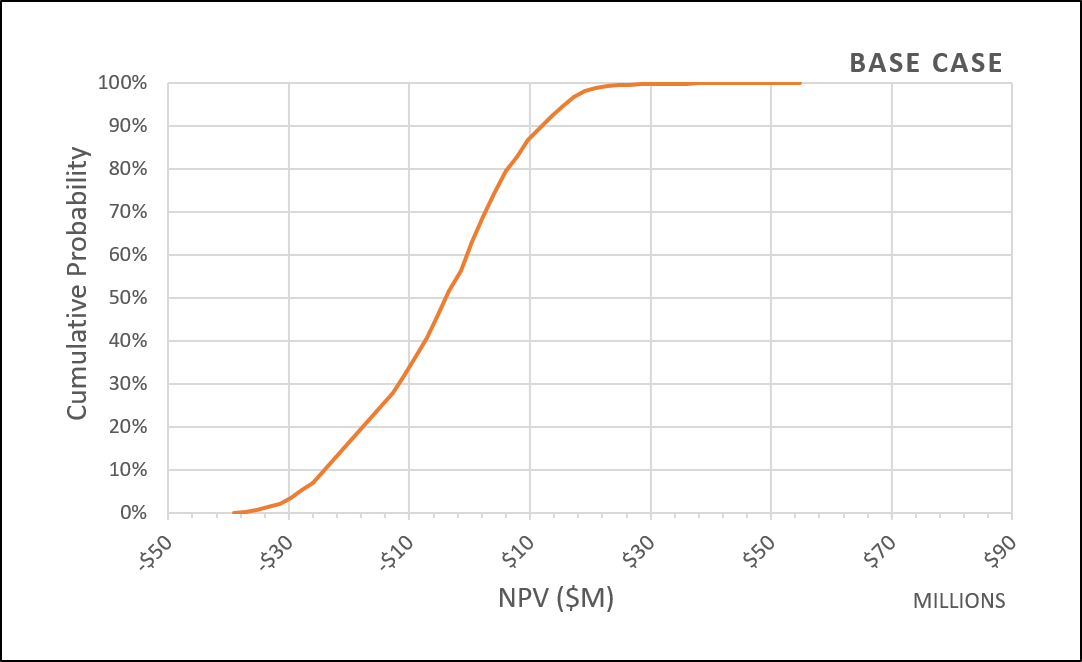
\includegraphics[width=.85\textwidth]{templates/images/Figure-Base_Case_CDF.png}
\caption[Base Case CDF]{Cumulative distribution function for the Base Case probabilistic cost model. The curve summarizes results from 2000 model realizations. NPV is reported in \$M, where M is million.}
\label{fig:base_case_cdf}
\end{figure}

All told, the Base Case results display both a negative ENPV and a high likelihood of project financial loss. Without a clear strategy for mitigating risk, this project would and should be rejected by a responsible portfolio manager.

\subsection{Summary Statistics}
\label{ch6:base_stats}

Table \ref{tab:base_stats} outlines key statistical measures summarizing the performance of the Base Case probabilistic cost model.

\begin{table}[H]
\centering
\begin{tabular}{|l|r|}
\hline
\textbf{Base Case Statistics} & N=2000 \\ \hline
ENPV & -\$4.8M \\ \hline
STD(NPV) & \$13.2M \\ \hline
P05 NPV & -\$28.2M \\ \hline
P50 NPV & -\$3.9M \\ \hline
P95 NPV & \$15.9M \\ \hline
\% Difference from NPV$_{s}$ & -565\% \\ \hline
\end{tabular}
\caption[Probabilistic Base Case statistics]{Base case probabilistic model statistics for 2000 model realizations. NPV is reported in \$M, where M is million. NPV$_s$ refers to the static model NPV, as reported in Table \ref{tab:static_mod_stats}.}
\label{tab:base_stats}
\end{table}

\section{Redevelop Case Model}
\label{ch6:redevelop_case}

The Redevelop Case model extends the Base Case with a redevelopment plan for the geothermal field to counter thermal decline in the fluid pathways through the reservoir. The Redevelopment decision rule (Section \ref{ch4:dr_redevelop}) is triggered when thermal drawdown causes the produced brine to drop below a threshold temperature. As with the Base Case, model uncertainties include drilling \& completions costs, electricity pricing, geothermal gradient, reservoir temperature, and thermal drawdown rate.

\subsection{Model Results}
\label{ch6:redevelop_results}

Adding the Redevelopment rule improves the project ENPV by \$2.3 million over the Base Case, but it still remains negative at -\$2.5 million, 340\% below the Static model NPV. Redevelopment drilling costs come into play as the VAG (P$_{05}$ value of \$15.1 million) decreases slightly relative to the Base Case. But VAR (P$_{95}$ value of \$21.3 million) shows a larger difference, improving by nearly \$7 million over the Base Case (Table \ref{tab:redevelop_stats}). This clearly reflects the improved production and power sales possible by managing reservoir conditions.

Standard deviation of the ensemble distribution is less than observed for the Base Case, likely due to a narrower overall distribution without as many outliers in the tails (Figure \ref{fig:redevelop_case_hist}). The balance in distribution shape is reflected in the small difference (\$0.2 million) between ENPV and the P$_{50}$ result (Table \ref{tab:redevelop_stats}). Comparing the target curves between the Redevelop Case (Figure \ref{fig:redevelop_case_cdf}) and Base Case (Figure \ref{fig:base_case_cdf}), it becomes clear that the redevelopment flexibility does not address upside potential. Instead, it acts as a partial stop-gap on the worst case realizations of the model. The lower half of the curve tightens up, but there is little overall curve movement to the right to make the project more profitable.

\begin{figure}[!htp]
\centering
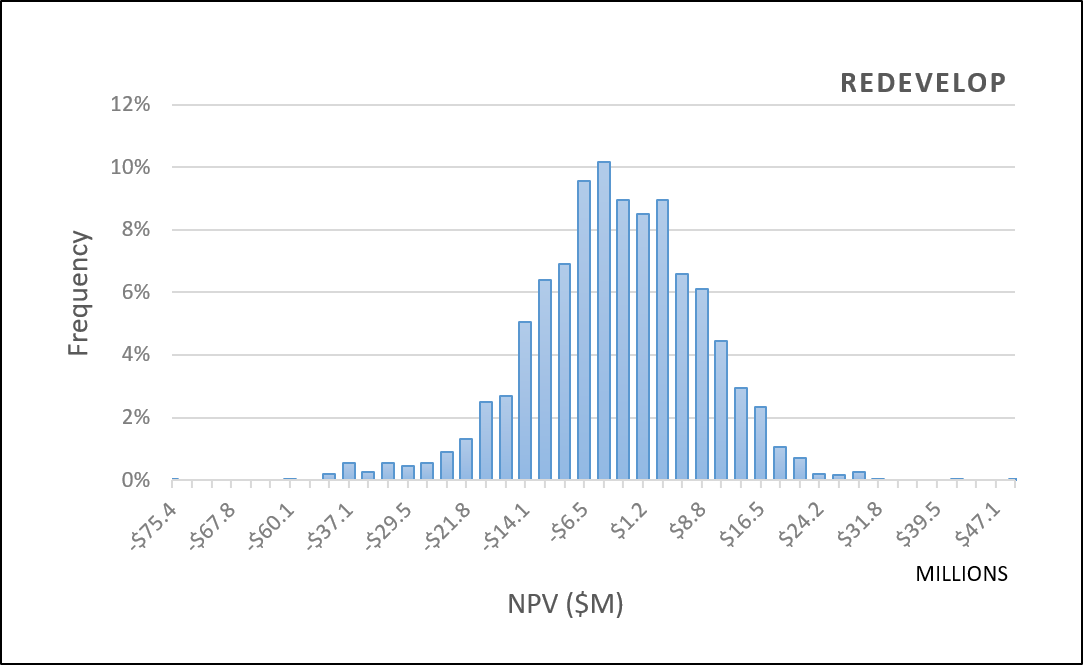
\includegraphics[width=.85\textwidth]{templates/images/Figure-Redevelop_Case_Histogram.png}
\caption[Redevelop Case histogram]{Redevelop Case probabilistic cost model histogram illustrating the distribution of 2000 model realizations. NPV is reported in \$M, where M is million.}
\label{fig:redevelop_case_hist}
\end{figure}

\begin{figure}[!htp]
\centering
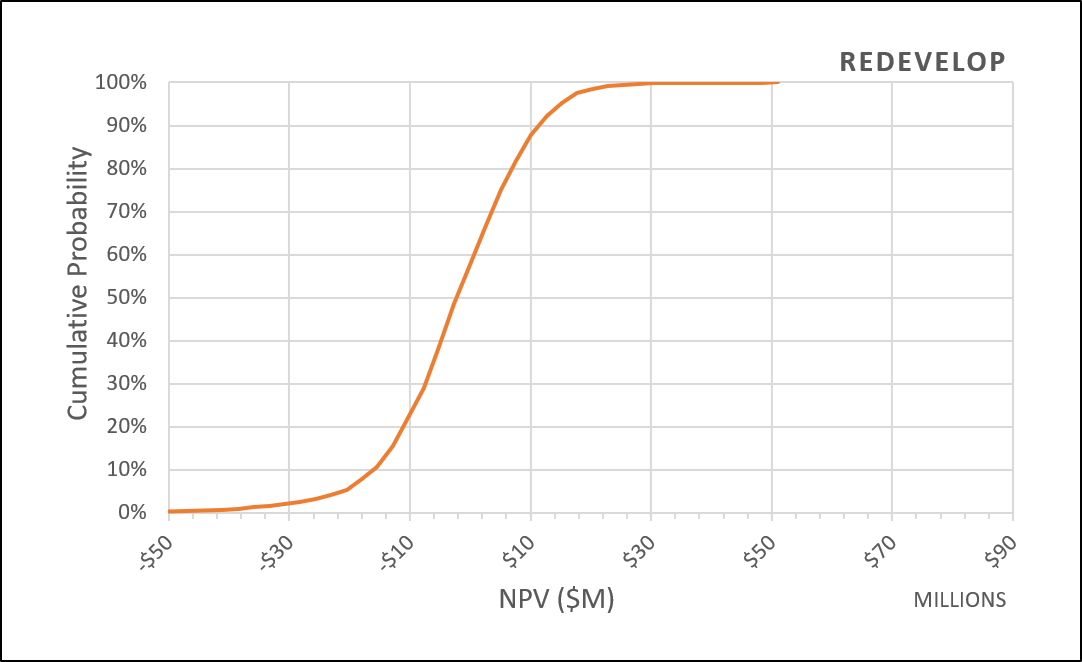
\includegraphics[width=.85\textwidth]{templates/images/Figure-Redevelop_Case_CDF.png}
\caption[Redevelop Case CDF]{Cumulative distribution function for the Redevelop Case probabilistic cost model. The curve summarizes results from 2000 model realizations. NPV is reported in \$M, where M is million.}
\label{fig:redevelop_case_cdf}
\end{figure}

As a brief caveat: the idea of periodic redevelopment for a geothermal field is not novel. In fact, many geothermal cost models include it as default behavior \citep[e.g.,\ ][]{entingh_volume_2006, blair_system_2018}. Nevertheless, the analysis above illustrates why this design option should be included in geothermal operations to help mitigate the risk of high thermal drawdown rates --- as long as drilling costs are low enough to make it attractive. 

\subsection{Summary Statistics}
\label{ch6:redevelop_stats}

Table \ref{tab:redevelop_stats} outlines key statistical measures summarizing the performance of the Redevelop Case probabilistic cost model.

\begin{table}[H]
\centering
\begin{tabular}{|l|r|}
\hline
\textbf{Redevelop Case Statistics} & N=2000 \\ \hline
ENPV & -\$2.5M \\ \hline
STD(NPV) & \$11.7M \\ \hline
P05 NPV & -\$21.3M \\ \hline
P50 NPV & -\$2.3M \\ \hline
P95 NPV & \$15.1M \\ \hline
\% Difference from NPV$_{s}$ & -344\% \\ \hline
\end{tabular}
\caption[Probabilistic Redevelop Case statistics]{Redevelop case probabilistic model statistics for 2000 model realizations. NPV is reported in \$M, where M is million. NPV$_s$ refers to the static model NPV, as reported in Table \ref{tab:static_mod_stats}.}
\label{tab:redevelop_stats}
\end{table}

\section{Redevelop \& Grow Case Model}
\label{ch6:grow_case}

The Redevelop \& Grow Case model builds on the Redevelop Case with a decision rule around increasing capacity (Section \ref{ch4:dr_grow}). Specifically, when electricity prices rise by an amount larger than the monitored threshold, more power plant modules are installed to capitalize on the increased prices and inferred demand. Like the other probabilistic models, values for drilling \& completions costs, electricity pricing, geothermal gradient, reservoir temperature, and thermal drawdown rate are directly sampled from probability distribution functions (Section \ref{ch4:pdfs}) as part of the Monte Carlo simulation.

\subsection{Model Results}
\label{ch6:grow_results}

Redevelop \& Grow model results use a field expansion amount of 25\% when the Capacity Growth decision rule is triggered. Assuming the PPA with the purchasing utility company is successfully renegotiated at the time of the expansion, this model results in a dramatic change in project value. ENPV is \$9.7 million, over \$12 million better than the Redevelop Case and over 800\% greater than Static model NPV (Table \ref{tab:grow_stats}). The case shows notable improvement in both Value at Risk and Value at Gain; P$_{05}$ shifts by more than \$7 million to -\$14.2 million, and P$_{95}$ leaps to \$38.2 million as power plant growth captures market potential.

\begin{figure}[!htp]
\centering
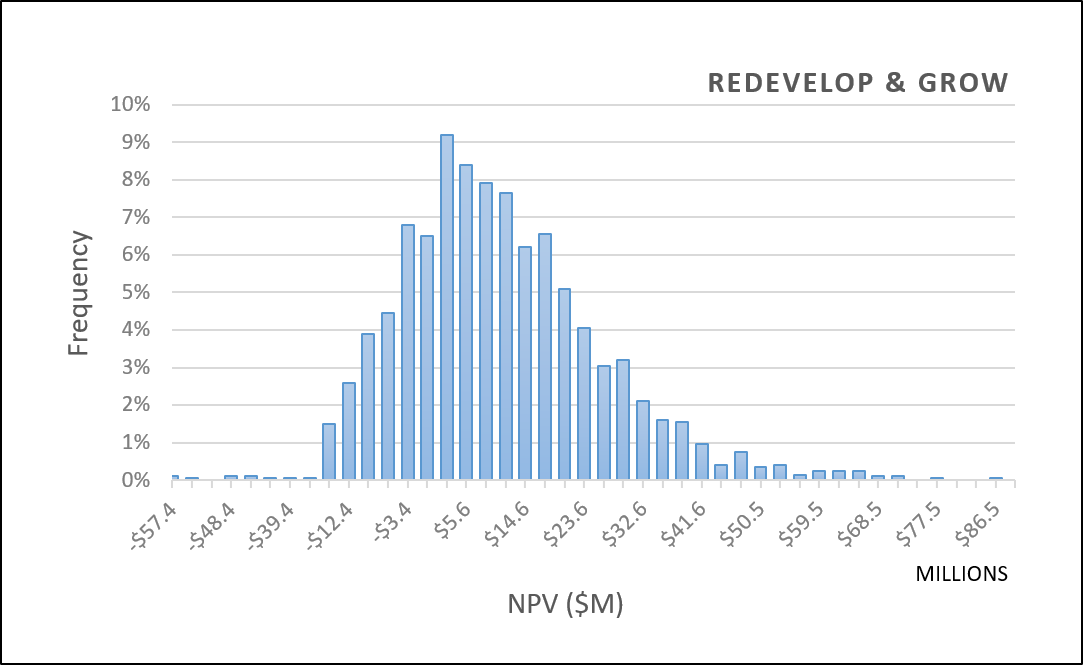
\includegraphics[width=.85\textwidth]{templates/images/Figure-Grow_Case_Histogram.png}
\caption[Redevelop \& Grow Case histogram]{Redevelop \& Grow Case probabilistic cost model histogram illustrating the distribution of 2000 model realizations. NPV is reported in \$M, where M is million.}
\label{fig:grow_case_hist}
\end{figure}

The histogram for Redevelop \& Grow skews noticeably to the right with a long tail of simulation runs marking high-value realizations of the model. Standard deviation of NPV increases compared to the Redevelop Only case, suggesting this model is less robust. However, the greater spread reflects more upside potential and is a desirable feature. It stands to reason then that robustness measured by standard deviation is not as useful a measure of design benefit as the other metrics in Table \ref{tab:grow_stats}. Figure \ref{fig:grow_case_cdf} illustrates the rightward shift of the target curve compared to those shown in Figures \ref{fig:base_case_cdf} and \ref{fig:redevelop_case_cdf}. Only 23\% of simulated results result in a project loss. 

\begin{figure}[!htp]
\centering
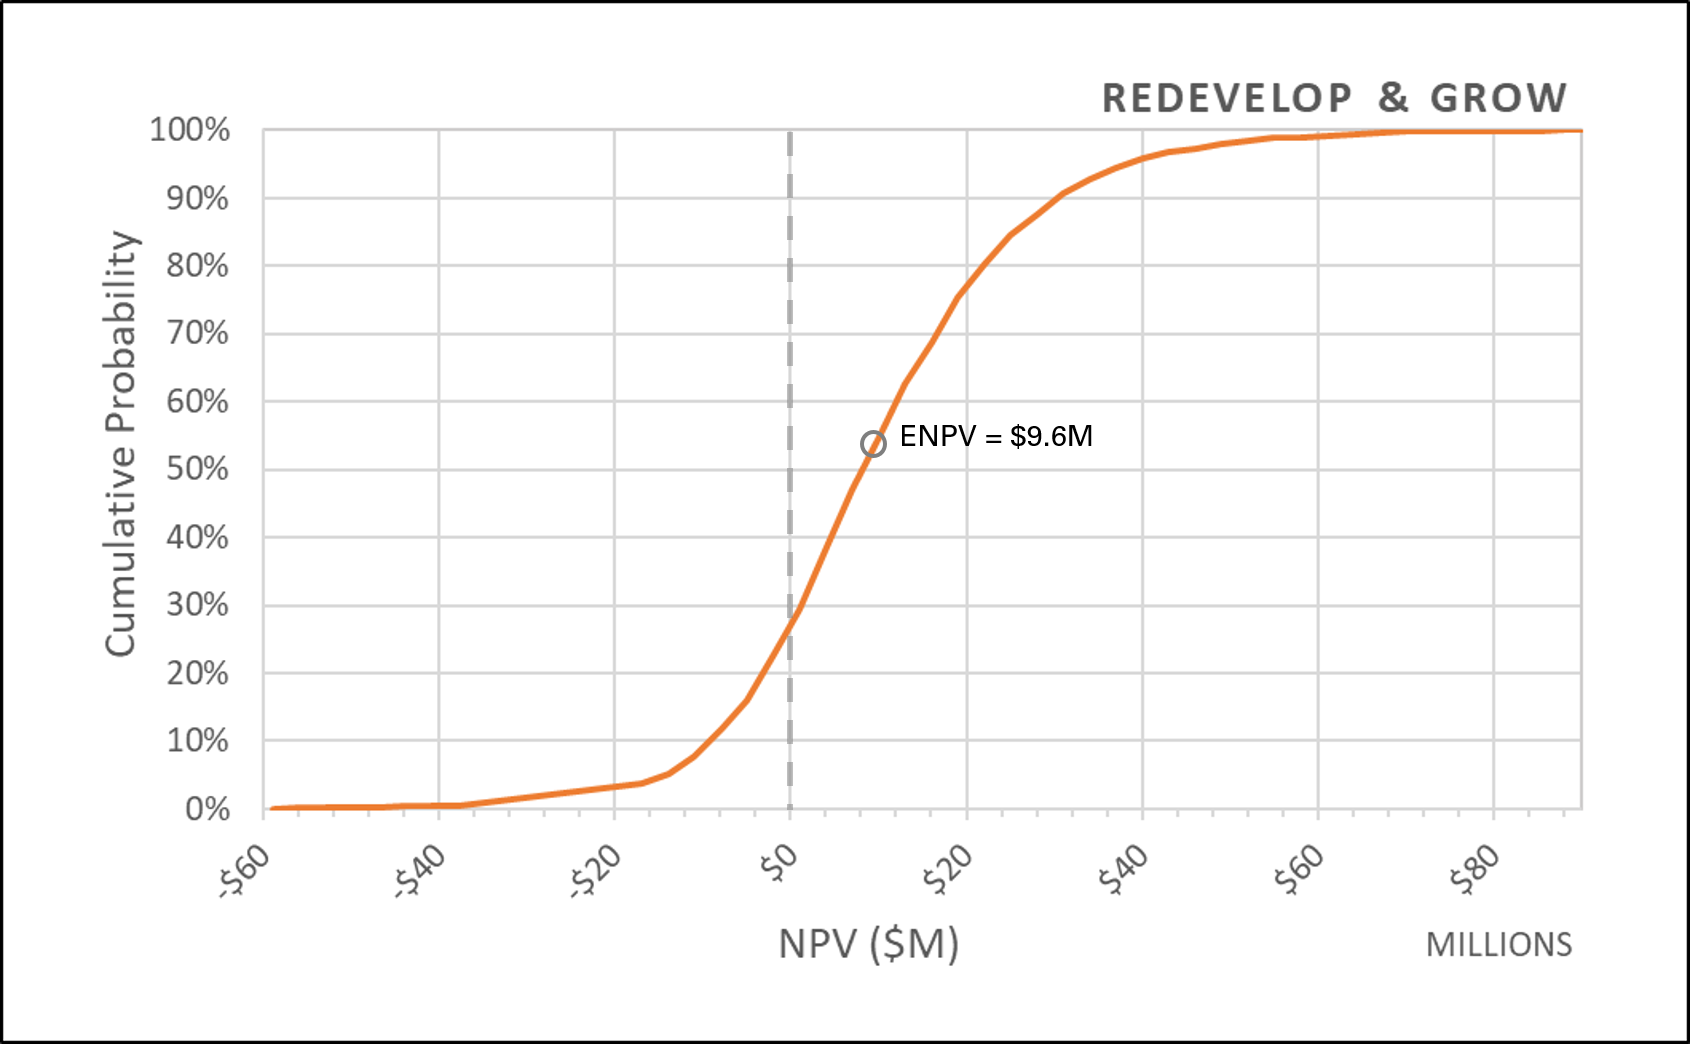
\includegraphics[width=.85\textwidth]{templates/images/Figure-Grow_Case_CDF.png}
\caption[Redevelop \& Grow Case CDF]{Cumulative distribution function for the Redevelop \& Grow Case probabilistic cost model. The curve summarizes results from 2000 model realizations. NPV is reported in \$M, where M is million.}
\label{fig:grow_case_cdf}
\end{figure}

Some caution should be taken in applying learnings from this model to a real-world geothermal project. Results here depend on a few important assumptions, including the willingness of a partner utility company to accept capacity increases above the market rate for electricity on any given year, the direct relationship between large price increases and electricity demand, and the overall monotonic increase in electricity prices over time. With regard to the latter, the price model used in this analysis includes a single step change and annual volatility (see Figure \ref{fig:elec_price_prob}), but other forecasts exist that depict negative year-on-year trends not modeled here \citep{murphy_electrification_2021}. As discussed in Section \ref{ch4:electrification_uncertainty}, the interactions between different energy markets and dynamics of major events like future electrification are complex, worth considering, and beyond the scope of this thesis. 

\subsection{Summary Statistics}
\label{ch6:grow_stats}

Table \ref{tab:grow_stats} outlines key statistical measures summarizing the performance of the Redevelop \& Grow Case probabilistic cost model.

\begin{table}[H]
\centering
\begin{tabular}{|l|r|}
\hline
\textbf{Redevelop \& Grow Case Statistics} & N=2000 \\ \hline
ENPV & \$9.6M \\ \hline
STD(NPV) & \$16.5M \\ \hline
P05 NPV & -\$14.2M \\ \hline
P50 NPV & \$8.2M \\ \hline
P95 NPV & \$38.2M \\ \hline
\% Difference from NPV$_{s}$ & 832\% \\ \hline
\end{tabular}
\caption[Redevelop \& Grow Case statistics]{Redevelop \& Grow case model statistics for 2000 model realizations. NPV is reported in \$M, where M is million. NPV$_s$ refers to the static model NPV, as reported in Table \ref{tab:static_mod_stats}.}
\label{tab:grow_stats}
\end{table}

\section{Full Flexibility Case Model}
\label{ch6:reduce_case}

Full Flexibility adds a decision rule around reduction of aggregate plant capacity (Section \ref{ch4:dr_reduce}). If electricity prices drop by a threshold amount, power plant modules are proactively decommissioned to reduce electricity production and operating expenses. Redevelopment and Capacity Growth decision rules remain in effect, as does the random sampling treatment for drilling \& completions costs, electricity pricing, geothermal gradient, reservoir temperature, and thermal drawdown rate based on PDFs defined in Section \ref{ch4:pdfs}.

\subsection{Model Results}
\label{ch6:reduce_results}

In a somewhat surprising outcome, the simulation for Full Flexibility results in an ENPV of \$6.7 million (Table \ref{tab:reduce_stats}). Although this value is 545\% greater than the Static model NPV, it falls short of the Redevelop \& Grow case by nearly \$3 million (see Table \ref{tab:grow_stats}). Both VAR and VAG show less attractive results as well; P$_{05}$ is -\$16.3M and P$_{95}$ is \$36.2 million, both $\approx \$2$ million worse than Redevelop \& Grow.  

\begin{figure}[!htp]
\centering
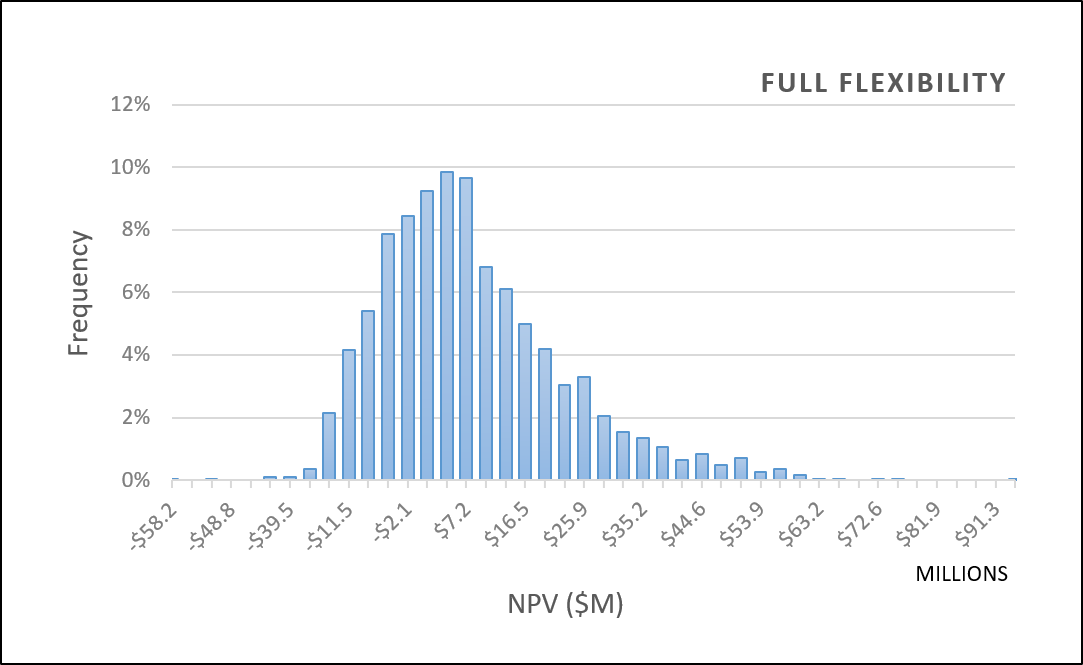
\includegraphics[width=.85\textwidth]{templates/images/Figure-Reduce_Case_Histogram.png}
\caption[Full Flexibility Case histogram]{Full Flexibility Case probabilistic cost model histogram illustrating the distribution of 2000 model realizations. NPV is reported in \$M, where M is million.}
\label{fig:reduce_case_hist}
\end{figure}

The results histogram (Figure \ref{fig:reduce_case_hist}) shows the same right skew as the Redevelop \& Grow model but with a slightly more compact form based on the lower standard deviation (Table \ref{tab:reduce_stats}). The difference in median values between the two cases amounts to $\approx\$3$ million, further confirming the Full Flexibility case is entirely dominated by the Redevelop \& Grow case. Figure \ref{fig:reduce_case_cdf} depicts the case target curve. There is a steep climb beginning at -\$14 million such that 33\% of model realizations result in project losses --- 10\% more than Redevelop \& Grow.

\begin{figure}[!htp]
\centering
\includegraphics[width=.85\textwidth]{templates/images/Figure-Reduce_Case_CDF.png}
\caption[Full Flexibility Case CDF]{Cumulative distribution function for the Full Flexibility Case probabilistic cost model. The curve summarizes results from 2000 model realizations. NPV is reported in \$M, where M is million.}
\label{fig:reduce_case_cdf}
\end{figure}

It is interesting to note that the modeled electricity forecast includes enough volatility to generate cases with both +20\% and -20\% price deviations (Figure \ref{fig:elec_price_prob}), potentially (and perhaps unrealistically) triggering both a capacity expansion and reduction within the same 30-year project lifespan. In addition, since modeled prices increase over time, except briefly when the randomly-placed step-change is negative, lost revenue from the utility forcing PPA renegotiations if electricity pricing went into a multi-year decline (e.g., Low Renewable Technology Cost case in Figure \ref{fig:EFS_electricification}) is not simulated here. These factors may play a role in the dominance of the Redevelop \& Grow case over Full Flexibility.

Nevertheless, there is an additional simple explanation for the model behavior. If power plant modules are decommissioned, the model is more sensitive to the drop in revenue from reduced electricity generation than any benefit realized by discounted OPEX. The cost savings is just not significant enough to make up for less income.

\subsection{Summary Statistics}
\label{ch6:reduce_stats}

Table \ref{tab:reduce_stats} outlines key statistical measures summarizing the performance of the Full Flexibility Case probabilistic cost model.

\begin{table}[H]
\centering
\begin{tabular}{|l|r|}
\hline
\textbf{Full Flexibility Case Statistics} & N=2000 \\ \hline
ENPV & \$6.7M \\ \hline
STD(NPV) & \$16.0M \\ \hline
P05 NPV & -\$16.3M \\ \hline
P50 NPV & \$4.9M \\ \hline
P95 NPV & \$36.2M \\ \hline
\% Difference from NPV$_{s}$ & 545\% \\ \hline
\end{tabular}
\caption[Full Flexibility Case statistics]{Full Flexibility case model statistics for 2000 model realizations. NPV is reported in \$M, where M is million. NPV$_s$ refers to the static model NPV, as reported in Table \ref{tab:static_mod_stats}.}
\label{tab:reduce_stats}
\end{table}

\section{Combined Model Comparison}

Figure \ref{fig:all_case_cdf} illustrates the target curves for the four (4) probabilistic models discussed in the previous sections. The Base Case model is dominated by all other models on the low-side and merges with the Redevelop Case on the high-side. The Full Flexibility Case greatly improves on the Base and Redevelop Cases. Redevelop \& Grow appears farthest to the right, making it the preferred model for the cost model parameterization as described in Section \ref{ch4:cm_params}. 

\begin{figure}[!htp]
\centering
\includegraphics[width=.85\textwidth]{templates/images/Figure-All_Case_CDF.png}
\caption[All Cases CDF]{Cumulative distribution functions for all probabilistic cases evaluated in Sections \ref{ch6:base_case} to \ref{ch6:reduce_case}. Each curve summarizes results from 2000 model realizations. NPV is reported in \$M, where M is million.}
\label{fig:all_case_cdf}
\end{figure}

\section{Full Flexibility Case Sensitivity Testing}
\label{ch6:sensitivity}

In order to explore the hypothesis that the Full Flexibility Case model is responding to revenue losses, a series of sensitivity tests considered adjustments to the \textit{Reduction amount} parameter controlling how many modules are removed by the Capacity Reduction decision rule (Table \ref{tab:cm_econ_params}, Section \ref{ch4:dr_reduce}). The default value applied throughout this analysis has been 25\% to match the \textit{Expansion amount} parameter used by the Capacity Growth decision rule (Table \ref{tab:cm_econ_params}, Section \ref{ch4:dr_grow}). Sensitivity testing with the \textit{Expansion amount} parameter is also conducted.

\subsection{Reduction Amount}
\label{ch6:sens_redamt}

The gap between the Full Flexibility (yellow) and Redevelop \& Grow (gray) curves broadens for higher \textit{Reduction amount} values. However, the curves begin to overlap for \textit{Reduction amount} values of $\leq{15}\%$. The difference is subtle, but the 5\% case shows a slight rightward step-out in the high-side values for Full Flexibility compared to the Redevelop \& Grow. This is not seen in the 4\% or 6\% scenarios, suggesting 5\% is the sweet spot for \textit{Reduction amount} when a significant electricity price drop is detected. For values above 5\%, the gain from OPEX reductions cannot overcome revenue lost from reduced capacity, which likely reflects the influence of PPA contracts that stabilize the year-to-year price paid for generated electricity. For values less than 5\%, the Full Flexibility Case merges with the Redevelop \& Grow Case as the number of decommissioned modules trends toward zero (0).

\begin{figure}[!htp]
\centering
\includegraphics[width=.98\textwidth]{templates/images/Figure-Sensitivity_Reduction.pdf.png}
\caption[Reduction Amount sensitivity test]{\textit{Reduction amount} sensitivity test using model target curves. Each curve illustrates results for a Monte Carlo simulation with 2000 runs of the indicated models. \textit{Reduction amount} only impacts Full Flexibility Case (yellow), so Base Case (orange), Redevelop Case (blue), and Redevelop \& Grow Case (gray) remain unchanged. \textit{Reduction amount values} include A. 35\%, B. 25\%, C. 15\%, D. 6\%, E. 5\%, and F. 4\%. NPV is reported in \$M, where M is million.}
\label{fig:sens_test_reduction}
\end{figure}

\subsection{Expansion Amount}
\label{ch6:sens_expamt}

A similar sensitivity test is executed by varying the \textit{Expansion amount} parameter while holding \textit{Reduction amount} at 5\%. Both the Full Flexibility and Redevelop \& Grow target curves respond to this parameter since both cases include the Capacity Growth decision rule (Section \ref{ch4:dr_grow}). Figure \ref{fig:sens_test_expansion} illustrates the results for step-wise increases to \textit{Expansion amount} by an increment of 20\%. 

Full Flexibility and Redevelop \& Grow target curves closely match each other except in the high-side model realizations, i.e., those above \$20 million NPV, and in the low-side near -\$20 million NPV. The low side variability relates to the sparse count of model realizations at -\$20 million NPV in each Monte Carlo simulation. For the better-constrained high-side, Full Flexibility shows a slight advantage when \textit{Expansion amount} is 25\% and 65\%. However, the separation is more pronounced for a 45\% \textit{Expansion amount}. In this sweet spot case, Full Flexibility ENPV amounts to \$13.7 million, $\approx\$1$ million greater than that for Redevelop \& Grow. This optimized potential would be missed without testing and refining the project growth and reduction strategies through sensitivity testing and parameter tuning.

\begin{figure}[!htp]
\centering
\includegraphics[width=.98\textwidth]{templates/images/Figure-Sensitivity_Expansion_Amount.png}
\caption[Expansion Amount sensitivity test]{\textit{Expansion amount} sensitivity test using model target curves. Each curve illustrates results for a Monte Carlo simulation with 2000 runs of the indicated models. \textit{Expansion amount} impacts both Redevelop \& Grow (gray) and Full Flexibility (yellow) target curves. Base Case (orange) and Redevelop Case (blue) remain unchanged. \textit{Expansion amount values} include A. 25\%, B. 45\%, and C. 65\%. NPV is reported in \$M, where M is million.}
\label{fig:sens_test_expansion}
\end{figure}

\section{Recap}\label{ch6:recap}
This chapter covered the execution of cost models described in Chapter \ref{ch4:cm_prep}. Results for a deterministic model and four (4) probabilistic models illustrate how incorporating uncertainties and decision rules into a modeling approach can provide important insights into potential project profit and loss. By comparing summary metrics and target curves, this methodology allows a decision-maker to test strategies for mitigating the risk of an unprofitable EGS expansion to an existing power plant.
\\
Key insights from cost modeling include:
\begin{enumerate}
    \item Static (deterministic) cost models that use average or most-likely parameter values are inherently flawed. They distort estimates of project value and may lead to poor project decisions.
    \item Probabilistic model result ensembles from Monte Carlo simulation are best compared using target curves (CDFs) and summary statistics like ENPV. Solution distribution robustness is not necessarily desirable --- imbalance toward the high side means a model has more Value at Gain.
    \item Redeveloping geothermal wells to counter reservoir thermal decline reduces downside risk but does not improve upside potential for the project.
    \item Installing additional power plant modules in response to greater demand results in significantly greater project value with reduced downside risk.
    \item Decommissioning power plant modules in response to plummeting prices generally does not capture greater project value, likely due to the lost revenue from reduced power generation outpacing savings in OPEX in this model formulation.
    \item Sensitivity testing of decision rule parameters is a means of optimizing operational strategy and can reveal hidden project value.
\end{enumerate}

\chapter{Discussion}\label{ch7:discuss}
\label{ch7:discussion}

Risk acts as a significant barrier to the adoption of geothermal as part of a larger energy portfolio for commercial oil \& gas companies. Here, the word \textit{risk} refers to the potential for shortfalls in performance with respect to established requirements, characterized by a probability of occurrence and consequence of failure \citep{nasa_s3001_2017, malone_development_2004}.  Companies considering investments in geothermal want to minimize risk exposure, so strategies to mitigate this risk will naturally act as enablers to geothermal growth during the on-going energy transition.

\section{Field Lifecycle}
\label{ch7:field_lifecycle}

Maturing a geothermal asset from initial concept through site decommissioning represents a complex project lifecycle spanning up to several decades in length. Figure \ref{fig:geothermal_field_lifecycle} illustrates the decomposition of a geothermal field lifecycle into a level 1 process flow that mimics that of a typical hydrocarbon field. The level 2 decomposition describes a work breakdown structure, each step with its own inherent risks. Here, the primary play risk elements for geothermal introduced in Section \ref{ch2:sysfund} have been reframed as four components: heat, permeability, fluids, and seal. Each appear in both the Exploration and Appraisal phases of the project. 

\begin{figure}
\centering
\includegraphics[width=\textwidth]{templates/images/Figure-SystemDecomposition.png}
\caption[Geothermal field lifecycle]{Proposed geothermal field lifecycle and two levels of decomposition defining major project phases and a high-level WBS. Dotted lines indicate where machine learning methods could mitigate risk in exploration and appraisal. Dashed lines depict where cost models might mitigate risk during the development and production phases.}
\label{fig:geothermal_field_lifecycle}
\end{figure}

The red dotted outline in Figure \ref{fig:geothermal_field_lifecycle} illustrates activities in the Exploration and Appraisal stages where machine learning methods described in Chapters \ref{ch3:expl_prep} and \ref{ch5:expl_ml} can reduce the overall risk profile. Geothermal exploration commonly focuses on areas where data and known resources are already present. Reviewing available data to identify feature relationships suggestive of favorable locations is an early pre-screening activity for mitigating the risk of costly exploration failures \citep{doughty_geovision_2018}. Machine learning algorithms described in Chapter \ref{ch5:expl_ml} provide data-driven methods for uncovering these complex feature relationships and generating resource favorability maps rapidly and at low cost. Furthermore, feature importances derived from recursive feature elimination (Section \ref{ch5:logreg_rfe}), impurity measures like Gini index or entropy (Section \ref{ch5:impurity}), or Shapley analysis (Section \ref{ch5:xgb_shapley}) directly rank different data sources by their value for predictive modeling. These measures could also be used to guide exploration and appraisal spending on additional data purchases or acquisition efforts. For example, recognizing that silica geothermometer temperatures, heat flow measurements, crustal thickness, and density of volcanic dikes and springs all highly influence the geothermal gradient classification model (see Section \ref{ch5:xgb_shapley}), an exploration team could focus time and budget on 1) field surveys for silica concentration sampling, 2) field or remote-sensing mapping of springs and dikes, and 3) seismic acquisition for improved crustal thickness estimates where those estimates are least well-constrained. As suggested by the black dotted line, the learnings from assessing geothermal heat content with machine learning techniques in Chapter \ref{ch5:expl_ml} are easily transferable to assessments for the other risk elements. 

Cost modeling similarly offers benefits for risk mitigation in the geothermal project lifecycle, as illustrated with the dashed lines in Figure \ref{fig:geothermal_field_lifecycle}. Surface plant construction and drilling activities take place during the development phase and continue into production as thermal decline or market forces trigger field management responses. Rather than treat the extent of these activities as known unknowns, characterizing and including them in flexible economic models offers the opportunity to assess their impact and scenario-test for the optimal field strategy. As the analysis in Chapter \ref{ch6:cm_results} showed, models can include local uncertainties, e.g., geothermal gradient or decline rate, as well as broader risks like a carbon tax or national electrification. The red long-dashed line in Figure \ref{fig:geothermal_field_lifecycle} surrounds factors considered by the cost model in Chapters \ref{ch4:cm_prep} and \ref{ch6:cm_results}. The gray dashed line depicts additional aspects of the development and production phases that could also be characterized in a cost model with distributions and decision rules to determine project viability or refine field strategy.

\section{Role of Uncertainty}
\label{ch7:uncertainty_role}

Uncertainty exists, as does the opportunity to include it in a larger decision-making process for geothermal adoption. In the exploration phase, feature standard errors and maps of entropy --- or another measure of collective uncertainty --- can influence project choices. Observing pervasively high standard errors for a data layer (see Section \ref{ch5:measure_uncertainty}) raises the question of whether that data should be re-acquired using different tools or survey methods, or if better quality data might be available for use or purchase. And zones of high entropy in measurement uncertainty highlight areas that need additional attention. Is the entropy a result of insufficient data to train machine learning models, leading to poor discrimination ability for the predicted classes? Or are the data in areas of high entropy simply inconclusive or poorly conditioned? Pursuing these questions helps frame a refined project plan for the early phases of the field lifecycle. In this scenario, time and resource allocations to data science and data engineering (using existing data), field studies and data acquisition (supplementing existing data), or exploration of more certain areas are expressly driven by the data.

If an ensemble of models is considered, structural or model uncertainty (see Section \ref{ch5:model_uncertainty}) can direct efforts around how to approach machine learning prediction. For example, when entropy appears high throughout the area of interest (AOI), and most of the models show reasonable agreement except for one or two, this could justify down-selecting those models and re-evaluating from the reduced ensemble. But if high variance is observed across many models, this might indicate the input data insufficiently describes the system. Likewise, predictions from probabilistic models that show high parameter uncertainty in the AOI (Section \ref{ch5:param_uncertainty}) should be treated as suspect and the model refactored or retrained on a larger data set. Insights like these mitigate the risk of over-confidence in under-performing models, potentially avoiding a poorly-placed exploration well based on those models further down the line.

For cost models, directly incorporating uncertainty serves to counter the classic misconception that applying average values to elements of a complex system will lead to an average system result \citep[Flaw of Averages,][p.\ 17-19]{de_neufville_flexibility_2011}. Instead, using variable distributions and generating expected values from multiple model realizations provides accurate median estimates and describes the spread of potential results. As discussed in Section \ref{ch6:cost_model_metrics}, target curves and percentiles defining Value at Risk and Value at Gain offer a richer set of metrics for model comparison. Using these metrics can reveal the combination of strategic choices for a geothermal project timeline and execution that mitigate the risk of project losses and captures the most potential gain.

\section{Risk Analysis}
\label{ch7:risk_analysis}

One approach to project risk assessment evaluates risks and mitigation actions with a scorecard tracking likelihood (Table \ref{tab:likelihood_table}) and consequence (Table \ref{tab:consequence_table}) of individual risks before and after actions are taken \citep{malone_development_2004}. The process begins with creating a risk log as shown in Table \ref{tab:risk_log}. This table can be constructed through a variety of risk identification methods, including formal hazard analysis, models and simulations, or group brainstorming \citep{nasa_s3001_2017}. Even the act of populating this table adds value to a project by building alignment on group judgment and assumptions regarding risk relevance and potential impact.

\begin{table}%[!htp]
\centering
\begin{tabular}{|c|l|c|}
\hline
\multicolumn{3}{|c|}{\textbf{Likelihood}} \\ \hline
\textbf{Score} & \multicolumn{2}{c|}{\textbf{Likelihood of Occurrence (p)}} \\ \hline
5 & Near certainty & (\ 0.8,1.0\ {]} \\ \hline
4 & Highly likely & (\ 0.6,0.8\ {]} \\ \hline
3 & Likely & (\ 0.4,0.6\ {]} \\ \hline
2 & Low likelihood & (\ 0.2,0.4\ {]} \\ \hline
1 & Not likely & {[}\ 0.0,0.2\ {]} \\ \hline
\end{tabular}
\caption[Risk likelihood]{Likelihood score based on probability of occurrence (p). Adapted from NASA S3001 Guidelines for Risk Management, v.G \protect\citep{malone_development_2004}.}
\label{tab:likelihood_table}
\end{table}

\begin{table}%[!htp]
\resizebox{\textwidth}{!}{
    \begin{tabular}{|l|L{0.17\linewidth}|L{0.17\linewidth}|L{0.17\linewidth}|L{0.17\linewidth}|L{0.17\linewidth}|}
    \hline
     & \multicolumn{5}{c|}{\textbf{Consequence}} \\ \hline
     & 1 & 2 & 3 & 4 & 5 \\ \hline
    \textbf{Performance} & Minimal to no impact on meeting project goals. & Minor impact on meeting project goals. & Unable to meet a specific project goal, but remaining goals can be achieved. & Unable to meet multiple project goals, but minimum project success still achievable. & Unable to meet multiple project goals, minimum project success not achievable. \\ \hline
    \textbf{Schedule} & Minimal to no impact on project schedule. & No change to critical milestones; at least 10-day buffer between any delay and impact on milestone timing. & No change to critical milestones; less than 10-day buffer between any delay and impact on milestone timing. & One or more critical milestones slip, impacting overall project schedule. & One or more critical milestones slip; one or more milestones cannot be achieved. \\ \hline
    \textbf{Cost} & Minimal to no impact on cost. & Minor impact on cost. Variance $< 5\%$ of total approved budget. & Impact on cost. Variance $> 5\%$ but $\leq 10\%$ of total approved budget. & Impact on cost. Variance $> 10\%$ but $\leq 15\%$ of total approved budget. & Major impact on cost. Variance $> 15\%$ of total approved budget. \\ \hline
    \end{tabular}
}
\caption[Risk consequence]{Consequence score defining the scale of impact a risk might have if it becomes a reality. Adapted from NASA S3001 Guidelines for Risk Management, v.G \protect\citep{malone_development_2004}.}
\label{tab:consequence_table}
\end{table}

\begin{table}%[!htp]
\resizebox{\textwidth}{!}{
    \begin{tabular}{|l|l|c|c|c|}
    \hline
    \multicolumn{1}{|c|}{\textbf{ID}} & \multicolumn{1}{c|}{\textbf{Description}} & \textbf{Likelihood} & \textbf{Consequence} & \textbf{Risk} \\ \hline
    EXP1 & Insufficient exploration budget & 4 & 3 & 12 \\ \hline
    EXP2 & Poor subsurface characterization & 4 & 4 & 16 \\ \hline
    EXP3 & Permitting delays & 3 & 3 & 9 \\ \hline
    DRL1 & Rig unavailability & 4 & 3 & 12 \\ \hline
    DRL2 & Drilling cost overruns & 3 & 3 & 9 \\ \hline
    DRL4 & Downhole equipment failure & 3 & 2 & 6 \\ \hline
    PRD1 & Insufficient production budget & 3 & 4 & 12 \\ \hline
    PRD4 & Rapid thermal decline & 3 & 4 & 12 \\ \hline
    PRD5 & Demand variability & 2 & 4 & 8 \\ \hline
    PRD6 & Wrong-sized infrastructure & 3 & 4 & 12 \\ \hline
    \end{tabular}
}
\caption[Geothermal risk log]{List of geothermal project risks, each assigned a likelihood of occurrence (see Table \ref{tab:likelihood_table}) and consequence (see Table \ref{tab:consequence_table}). Risk is likelihood $\times$ consequence. This list is non-exhaustive and intended to support discussion of risk matrix use.}
\label{tab:risk_log}
\end{table}

Having captured risks and ordered them by their risk score, the project team next defines mitigation plans for addressing those risks (e.g., Table \ref{tab:mitigation_log}). The resulting \textit{mitigated} risks are analyzed and assigned updated scores for likelihood and consequence, which also define the remaining risk value. Different mitigation options for the same risk can be directly compared by the final risk scores or individual likelihood or consequence scores if addressing one over the other is preferred.

\begin{table}[!htp]
\renewcommand{\arraystretch}{2.5}
\resizebox{\textwidth}{!}{
    \begin{tabular}{|l|M{0.12\linewidth}|M{0.12\linewidth}|M{0.12\linewidth}|M{0.12\linewidth}|L{0.42\linewidth}|}
    \hline
    \multicolumn{1}{|c|}{ID} & Mitigated Likelihood & Mitigated Consequence & Mitigated Risk & Risk Reduction & Mitigation Action \\ \hline
    \rowcolor[HTML]{E7E6E6} 
    EXP1 & 1 & 2 & 2 & 10 & Use ML model predictions to reduce costs in exploration \\ \hline
    \rowcolor[HTML]{E7E6E6} 
    EXP2 & 1 & 3 & 3 & 13 & Use ML for baseline model, acquire data based on importances \\ \hline
    EXP3 & 2 & 3 & 6 & 3 & Engage with regulators early to fast-track permitting \\ \hline
    DRL1 & 3 & 3 & 9 & 3 & Secure rig early and pre-plan for future drilling needs \\ \hline
    \rowcolor[HTML]{E7E6E6} 
    DRL2 & 1 & 3 & 3 & 6 & Use ML to identify high gradient areas faster, shallower drilling \\ \hline
    DRL4 & 2 & 2 & 4 & 2 & Use service companies with high-Temp equipment track record \\ \hline
    \rowcolor[HTML]{E7E6E6} 
    PRD1 & 1 & 3 & 3 & 9 & Cost modeling for optimized spending and return \\ \hline
    PRD4 & 3 & 2 & 6 & 6 & Regularly re-drill wells or re-stimulate reservoir \\ \hline
    \rowcolor[HTML]{E7E6E6}
    PRD5 & 2 & 2 & 4 & 4 & Flexibility in power generation based on market \\ \hline
    \rowcolor[HTML]{E7E6E6}
    PRD6 & 1 & 2 & 2 & 10 & Flexible design for demand-triggered capacity changes \\ \hline
    \end{tabular}}
\caption[Geothermal mitigation log]{Proposed mitigations for risks listed in Table \ref{tab:risk_log} and the change in risk associated with those mitigations. Risk values are likelihood $\times$ consequence. Shaded mitigations include one of the options described in this thesis and appear in Figure \ref{fig:risk_matrix}. Adapted from NASA S3001 Guidelines for Risk Management, v.G (Malone \& Moses, 2004). }
\label{tab:mitigation_log}
\end{table}

The risk scorecard methodology plots risks before and after mitigation on a $5\times5$ matrix, where high-likelihood, high-consequence risks fall near the upper-right, and the lower-left represents the ideal low-likelihood, minimal-consequence region. The risk matrix serves two main functions: prioritization and selection. First, it quickly differentiates between risks by using assigned risk priorities for each matrix cell. Following NASA guidelines, priority values across the matrix increase toward the upper-right, are non-symmetric, and skew higher for high-consequence cells \citep{nasa_s3001_2017}. Secondly, different mitigation strategies for the same risk can be evaluated and plotted in the same $5\times5$. This helps quickly communicate relative outcomes of different strategies and supports rapid decision-making on which to select.

\begin{figure}%[htp]
\centering
\includegraphics[width=\linewidth]{templates/images/Figure-Risk_Matrix.png}
\caption[Geothermal project risk matrix]{Risk matrix for categorizing and prioritizing project risks (dark gray) and charting risk mitigation strategies (white). Marker size corresponds with risk value (likelihood $\times$ consequence). Markers are spread out within each cell for visualization purposes. Risk labels match those in Table \ref{tab:risk_log}.}
\label{fig:risk_matrix}
\end{figure}

Figure \ref{fig:risk_matrix} illustrates a risk matrix based on the highlighted rows from Table \ref{tab:mitigation_log}. Arrows map the original risk to mitigated risk. Each of these examples utilizes mitigation strategies described in the earlier chapters of this thesis. Although many other geothermal project risks exist than those described here, what this work demonstrates is the ability \textit{to} reduce risk \textit{by} rapidly applying low-cost assessments throughout the lifecycle of a geothermal field \textit{using} readily-available data. At the exploration stage, machine-learning PFA assessments feed directly into risking processes already common in oil \& gas companies \citep{nash_adaptation_2015}. This reduces barriers around deployment and adoption, and the risk reduction in Figure \ref{fig:risk_matrix} clearly demonstrates the potential value gained. In the development and production stages, use of scenario-testing with flexible cost models mitigates risk while possibly revealing new, more profitable means of operating a geothermal field. And doing so with spreadsheet-based tools means petroleum industry project managers already have the technology and capability to apply these models for decision-support and risk-mitigation today. 

\section{Great Opportunity}

Oil \& gas companies are uniquely positioned to embrace geothermal, including EGS, as a low-carbon baseload option in the energy transition. Consider some present-day barriers to broad commercial development of EGS described in the GeoVision study: 
\begin{enumerate}
    \item \textit{Companies advancing EGS are small, lacking significant operating capital and the ability to tackle large-scale projects (>100 MW)} \citep{doughty_geovision_2018}. Oil \& gas companies have the working capital to take on larger, more expensive projects if those projects have the potential for long-term profitability.
    \item \textit{Subsurface characterization with advanced methods like seismic imaging and reservoir modeling require capabilities not generally found in the geothermal industry} \citep{doughty_geovision_2018}. Use of the most advanced geophysical data processing techniques, cutting-edge interpretation platforms, and 3D earth modeling methods are standard practice in the petroleum industry.
    \item \textit{Geothermal practitioners lack standardization or best practices for drilling complex wells} \citep{doughty_geovision_2018}. Oil \& gas companies follow standard procedures in drilling operations founded on years of experience drilling wells all across the globe, including in environments challenged by extreme depths, complex geology, and high temperatures and pressures.
    \item \textit{EGS requires complex subsurface operations like directional drilling and multi-zonal isolation for fracture stimulation not typical of traditional hydrothermal operations} \citep{augustine_geovision_2019}. Technology improvements and years of expertise gained from developing unconventional reservoirs have created a wealth of experience in directional drilling and fracking within the oil \& gas industry.
\end{enumerate}

Interest in collaboration runs high as well. The Geothermal Technologies Office regularly promotes cross-over technology transfer between the oil \& gas and geothermal communities, funding programs like GEO out of the University of Texas Austin that specifically target transitioning industry capabilities \citep{hamm_geothermal_2021}. And the operational efficiencies that companies like Unocal previously brought to geothermal operations in the United States, Philippines, and Indonesia in the past resonate with the needs of today \citep{melosh_geothermal_2017,palma_dynamic_2014}.

Given the promise of change in the energy transition, the cross-sector synergies in fundamental skill sets, and strong interest in partnership from those already committed, geothermal may be the shortest path solution for building a lower-carbon business portfolio. Getting there requires analysis of the risks as well as mitigation strategies needed to reduce the likelihood and consequence of those risks, as described in Section \ref{ch7:risk_analysis}. Based on the results of this thesis, the path from great opportunity to profitability may lie in combining available data and digital technologies to create useful predictive models with uncertainty. The last part is fundamental --- uncertainty analysis will define where measurements are meaningful, where models are predictive, and which strategy offers the greatest potential gain. Lessons learned here apply to geothermal exploration and production, but embracing uncertainty for better decision-making and risk-mitigation will likely benefit every stage of the geothermal lifecycle. Uncertainty characterization may thus be the key to building more certainty in the future of geothermal.
\chapter{Conclusions}\label{ch8:conclusions}
As the transition toward lower-carbon energy solutions continues to progress, geothermal uniquely offers a zero-emissions, continuous source that can fulfill the baseload needs of energy consumers. A geothermal field lifecycle closely follows that of a hydrocarbon field, from exploration and appraisal, through field development, to production and eventual decommissioning. The expertise with subsurface data, reservoir modeling, complex drilling, and field management skills valued in oil \& gas are similarly of great value to the geothermal industry. However, geothermal without EGS only has limited reach, and EGS comes with high risk. Without clear risk-mitigation strategies, oil \& gas will likely discount or delay adding geothermal to their energy portfolios despite the clear synergies between the two domains.

Play fairway analysis, a common tool in the oil \& gas industry, has gained traction for reducing risks associated with geothermal exploration. However, PFA requires integration of disparate data sets to define chance of success for geothermal risk elements. This process lacks standardization and requires judgment calls from subject matter experts. Machine learning offers data-driven forecasts that are both quantitative and repeatable, and results from this work shows great promise in the predictive ability of several varieties of machine learning models. Perhaps more importantly, uncertainty characterization delivers invaluable information on where the data should be trusted, where predictive capacity of individual models varies, and where multiple models agree. Furthermore, machine learning models determine which data sets provide the most discriminatory value, which can steer exploration spend on additional data acquisition activities. Collectively, use of machine learning for play-risking or prospecting reduces the risk of making poor decisions on unreliable favorability maps, allocating budget on low-impact data sets, or missing important signals within the data that make the difference between a productive or an uneconomic geothermal well. And by relying on available data up-front to build these models, machine learning-based risk-mitigation comes with quick results at low cost.

Geothermal cost modeling with existing tools delivers levelized cost estimates from a set of pre-determined resource, surface plant, field, and financial parameters for the production phase of a field. Yet most of these models disallow defining input parameters with a distribution of values capturing parameter uncertainty. In addition, the models assume static operational conditions over the lifetime of the field (typically 30 years), which leaves no room for the strategic decision-making that takes place under real-life conditions. This thesis shows economic modeling that includes parameter uncertainties produces easily-comparable probabilistic distributions as results. Tailoring the model and decision rules to the geothermal field design of interest allows rapid testing of project feasibility and optimization of project actions to limit downside risk while capturing upside potential. Risks are addressed transparently and with quantifiable project impact at little cost in resources or capital.

Mitigating the risks of adopting geothermal energy should be handled systematically through a risk management process. Working within a geothermal project team, risks are cataloged, assigned likelihood and consequence values, and prioritized based on those values using a risk matrix. Choosing among mitigation plans comes down to comparing the results of executing each proposed plan of action. As shown by the work presented here, mitigation plans that combine available data with digital technologies to create predictive models with uncertainty can significantly reduce the threat of high-consequence geothermal exploration and production risks. Careful uncertainty characterization and evaluation may thus be the key to making geothermal a commercially-viable, low-carbon investment for oil \& gas companies navigating an evolving energy future. 
\chapter{Future Work}
\label{ch9:future_work}

In this chapter, directions of further inquiry are suggested as both extensions of methods already reviewed and new avenues not yet explored by the author. The topic of geothermal energy is a rich one with many great opportunities for research.

\section{Machine Learning Applications}\label{ch9:future_work_ml}

This thesis primarily focused on supervised classification models in its survey of machine learning methods for geothermal exploration. Maintaining a limited scope in modeling -- as well as in data-gathering and preparation --- was intentional, but doing so set aside a number of topics worthy of follow-up analysis:

\begin{itemize}
    \item Machine learning methods in Chapter \ref{ch5:ml_results} framed the prediction problem as a classification with four distinct labels for assignment (see Section \ref{ch3:gradient_classes}). Although convenient, this choice is problematic for continuous response variables like geothermal gradient. Classifiers treated each gradient class as independent, with no inherent ordered relationship. This assumption is of course false. Binning continuous variables makes sense when training data is sparse, but care must be taken for cases near the bounds between those bins. Further research on applying regression methods would help answer whether similar machine learning tools can perform well at predicting those edge case gradients where even the best classifiers (XGBoost, ANN) appeared to have difficulty.
    \item Choosing to use point data extracted from geothermal feature maps as input to machine learning models (see Section \ref{ch3:meshgrid}) was expedient, but it also ignored the spatial correlation inherent to geologic data. The presence of features like faults or volcanic dikes at one location naturally raises the probability of finding the same at a nearby location. This kind of spatial relationship might be better preserved using convolutional neural networks or more complex network architectures that go beyond the fully-connected ANN described in Section \ref{ch5:ann_structure}.
    \item Management of data sparsity is a common issue in exploration. Here, the original data set was augmented by imputed pseudo-wells (Section \ref{ch3:imputation}) in a crude but effective approach to expanding the training data set. Data imputation using more elegant and advanced methods would be a worthwhile topic of study for defining standards and recommendations to guide future geothermal data engineers.
    \item Autoencoders, Principle Component Analysis, and Non-negative Matrix Factorization are all effective tools for dimensionality reduction. Evaluating these and other methods can help bridge the gap between the supervised studies in this thesis and unsupervised efforts described in recent literature \citep{pepin_new_2019,smith_characterizing_2021,vesselinov_discovering_2020}. Of particular interest might be consolidating many features associated with the same geothermal risk element into “super features” before applying tree-based ensemble methods or neural networks for classification.
    \item Uncertainty estimation for secondary data products, e.g. raster files generated by others without paired standard errors or original primary-source observations, will be necessary to evaluate measurement uncertainty (see Section \ref{ch5:measure_uncertainty}) for all modeled features. Until the day that reporting uncertainties becomes an expectation, if not a requirement, there will be the need for clear guidance on deriving error estimates for pre-gridded data.
    \item The topic of ensemble models was raised in this thesis but not rigorously pursued. Ensemble models apply a model-of-models paradigm to machine learning and show success in other applications \citep[e.g.,][]{wilson_machine_2020}. They naturally tie to Play Fairway Analysis where final favorability maps represent combinatory insights from individual risk element maps (see Section \ref{ch2:pfa}). An ensemble model approach could streamline creation of a final geothermal favorability map while also preserving the prediction of specific risk components.
\end{itemize}

\section{Cost Modeling}\label{ch9:future_work_cm}

Although a number of economic models for geothermal power production already exist with varying degrees of maturity (see Section \ref{ch2:cost_models}), the contribution of this thesis to incorporating uncertainty and flexibility into cost models merely scratches the surface on what can still be done.

\begin{itemize}
    \item Using well-known, popular platforms like Microsoft Excel greatly lessens the burden around deployment and adoption of new tools. However, spreadsheets come with limitations, some of which impacted the capabilities of the cost model defined in Section \ref{ch4:cm_concept}. Most significantly, the individual power plant modules and injector-producer well couplets were difficult to track and manage as their count dynamically changed throughout the lifespan of a field. One suggested improvement is to expand the existing model with more complex code that treats the modules and wells as objects, each with individually-tracked attributes like age, efficiencies, decline rates, and maintenance records. Uncertainty definitions, decision rules, and overall user experience can remain Excel-based, but functionality enhancements via an Excel plug-in or VBA code could overcome calculation limitations.
    \item Electricity pricing forecasts and Power Purchase Agreements (PPAs) likely require a more nuanced treatment than conducted in this thesis. Additional research into the best representation of wholesale electricity price changes, including reversing trends, would be a good first step. But perhaps more fundamentally, the relationship between price changes and the likelihood and scope of a PPA update with utility partners must be characterized and modeled.
    \item The Electrification Futures Study \citep{murphy_electrification_2021} and the SIPA study on carbon taxation \citep{larson_energy_2018} both note complexities of modeling renewable energy demand when the growth and impact of the natural gas market remains uncertain. Furthermore, the role of targeted subsidies for technologies like wind energy further disrupt an already tilted playing field \citep[see][]{lazard_lazards_2020}. As cost models for geothermal continue to be refined, the dynamics associated with the natural gas market and incentives (including subsidies) for other competing renewables must be incorporated into an overall demand equation. The latter can help determine field expansion strategies and influence the agreed-upon pricing for PPA updates.
    \item A unique feature of the cost model described in this thesis is the treatment of power plant installation and expansion as modular in nature. This concept builds on existing technology, but the companies leading the way with that technology treat aspects of its performance and their financial terms of service as trade secrets. More accurate data regarding module up-front costs, performance limits for higher-temperature production, and fee structure for leasing, expansion, and decommissioning would all improve the existing model.
    \item Other opportunities for enhancing the geothermal cost model include: split pricing for electricity sales in addition to the original PPA with a utility, identifying and capturing efficiencies (e.g. lower fluid costs) from the expansion nature of the plant being modeled, incorporating local sales to nearby businesses or towns as separate revenue streams, and investigating how hybrid power (paired solar, wind) and storage (battery) project options influence the bottom line.
\end{itemize}

\section{Related Research Topics}\label{ch9:future_work_related}

\begin{itemize}
    \item The original scope of this thesis included a section on evaluating existing and future drilling technologies. One possible roadmap for this research effort follows a systems approach. System architectural analyses of innovative techniques like millimeter-wave drilling \citep{woskov_millimeter-wave_2017} or spallation drilling \cite{augustine_hydrothermal_2009} could be compared to expected improvements to traditional rotary drilling \citep{lowry_geovision_2017}. Feedback from geothermal stakeholders would calibrate the benefit side of a cost-benefit analysis that includes constructing a tradespace to select preferred drilling architectures. As an added bonus, detailed cost estimates derived in the process could help reduce drilling cost uncertainty for geothermal cost models.
    \item Machine learning methods used to generate map-based assessments of favorability lack the specificity of a 3-D subsurface model. Many of the geothermal data features described in Chapter \ref{ch3:data_prep} refer to surface observations. However, geophysical techniques (seismic, resistivity, gravity, magnetic, MT measurements) and interpretation products (faults, horizons, rock properties) typically extend into the third dimension. Research into transitioning a 2-D PFA into a 2.5- or 3-D analysis would help bridge the gap between the needs of mapping plays and those of full prospect characterization and detailed field planning.
    \item Significant efforts have already been made in gathering geothermal-related data for access through the NREL OpenEI \citep{hallett_open_2010} or Geothermal Prospector \citep{nrel_geothermal_2021} data portals. With more data available, including those from large-scale integrated EGS projects like Utah FORGE \citep{moore_utah_2019}, research on effective reservoir characterization methods, early field operations, and sustaining field management will serve to increase efficiencies across the geothermal lifecycle. This research will be a fundamental factor toward broadly commercializing EGS.
\end{itemize}
\appendix
\chapter{Appendix A}

\clearpage
\newpage

\chapter{Cost Model Spreadsheets}\label{app:B_cost_model_spreadsheets}

\section{Static NPV Model}\label{app:B_static_model}
The static model described in Section \ref{ch4:cm_concept} was implemented in Microsoft Excel as a single sheet for cost analysis. Figures \ref{fig:static_model_sheet1} and \ref{fig:static_model_sheet2} show the model when flow rate is pre-defined and capacity depends on the input temperature of the produced brine. Not shown is the supporting look-up table for the EIA STEO-based electricity price forecast (Figure \ref{fig:electricity_pricing}).
\vfill
\pagebreak

\begin{figure}[H]
\centering
\includegraphics[width=\textwidth]{templates/images/Figure-Static_Model_SheetA.png}
\caption[Static cost model worksheet (part 1)]{First part of geothermal power plant expansion static NPV cost model.}
\label{fig:static_model_sheet1}
\end{figure}

\begin{figure}[H]
\centering
\includegraphics[width=\textwidth]{templates/images/Figure-Static_Model_SheetB.png}
\caption[Static cost model worksheet (part 2)]{Second part of geothermal power plant expansion static NPV cost model. The yearly breakdown of cost and revenue only extends out to year 2 for visualization purposes but continues to year 30 in the actual spreadsheet.}
\label{fig:static_model_sheet2}
\end{figure}
\pagebreak
\section{Flexible NPV Models}\label{app:B_flex_models}

\textbf{TO BE ADDED}
\addcontentsline{toc}{chapter}{References}
%% This defines the bibliography file (main.bib) and the bibliography style.
%% If you want to create a bibliography file by hand, change the contents of
%% this file to a `thebibliography' environment.  For more information 
%% see section 4.3 of the LaTeX manual.
\begin{singlespace}
\bibliography{main}

%% APA citation
\bibliographystyle{apacite}
\end{singlespace}

\end{document}
